\documentclass[11pt,DIV=13,BCOR=5mm,a4paper,headinclude,pointlessnumbers]{scrbook}
%\usepackage[ngerman]{babel}
\usepackage[english]{babel}
\usepackage[utf8]{inputenc}
\usepackage[T1]{fontenc}
\usepackage{lmodern}
\usepackage{upgreek}
%\usepackage{graphicx}
\usepackage[figuresright]{rotating}	% lädt auch graphicx
\usepackage{caption}
 \DeclareCaptionLabelFormat{myformat}{#1~#2}
% \captionsetup{labelformat=myformat}
\usepackage{xcolor}
\usepackage{amsmath}
\usepackage{amssymb}
\usepackage[version=3]{mhchem} % Formula subscripts using \ce{}
\usepackage{setspace}
\usepackage{titletoc}
\usepackage{scrpage2}
\usepackage{textcomp}
\usepackage{ragged2e}
\usepackage{booktabs}
\usepackage{threeparttable}
\usepackage[sf,SF]{subfigure}
\renewcommand\thesubfigure{\,(\alph{subfigure})}
\usepackage{rotating}
\usepackage{enumitem}
\usepackage{multirow}
\usepackage{color}
% \usepackage{ulem}
\usepackage{etoolbox}
\usepackage{bibentry}
\usepackage{placeins}
\usepackage{cite}
% \usepackage[superscript,biblabel]{cite}
% Hurenkinder und Schusterjungen verhindern
\clubpenalty10000
\widowpenalty10000
\displaywidowpenalty=10000

%\nobibliography*

\clubpenalty = 10000
\widowpenalty = 10000

\linespread{1.25}
\KOMAoptions{DIV=last}

%Links im Inhaltsverzeichnis
\usepackage{hyperref}
\hypersetup{colorlinks,citecolor=black,filecolor=black,linkcolor=black,urlcolor=black}

%Eigene Befehle
\newcommand*{\mystrut}{\rule[-.2\baselineskip]{0pt}{-.2\baselineskip}}
\renewcommand*{\dictumwidth}{0.618\textwidth}
\renewcommand*{\partpagestyle}{empty}
\setlength{\parskip}{0pt}
\newcommand\todo[1]{\textcolor{red}{TODO: \textit{{#1}}}}

%Eigene Mathebefehle
\def\mathbi#1{\textbf{\em #1}}
\renewcommand{\vec}[1]{\underline{#1}}
\renewcommand{\i}{{\mathrm{i}}}
\addtokomafont{disposition}{\boldmath}
\def\doubleunderline#1{\underline{\underline{#1}}}

%Überschriften
\addtokomafont{part}{\huge}
\addtokomafont{chapter}{\LARGE}
\addtokomafont{section}{\Large}
\addtokomafont{subsection}{\large}
\addtokomafont{subsubsection}{\large\sffamily\textit}

%Captions anpassen
\setcapindent{1em}
\setkomafont{captionlabel}{\sffamily\bfseries}
\setkomafont{caption}{\sffamily}
%\addtokomafont{caption}{\small\sffamily}
\KOMAoption{captions}{outerbeside}

%Fußnoten
\usepackage[bottom,hang]{footmisc}
\setlength{\skip\footins}{\baselineskip}
\setlength{\footnotesep}{0.75\baselineskip}
\deffootnote[1.0em]{0.0em}{1.0em}{\textsuperscript{\thefootnotemark~}}

%Listen anpassen
\setlist[enumerate]{rightmargin=\leftmargin,noitemsep,label=(\arabic*)}

%Boxen anpassen
\setlength{\fboxsep}{0pt}
\setlength{\fboxrule}{1pt}

%Kopfzeile
\pagestyle{scrheadings}
\clearscrheadfoot
\renewcommand*{\partmarkformat}{}
\automark[section]{chapter}
\lehead[]{\leftmark}
\rohead[]{\rightmark}
\lefoot[\pagemark]{\pagemark}
\rofoot[\pagemark]{\pagemark}

%Appendix
\newcommand*{\appendixmore}{
% \renewcommand{\thesection}{\Alph{section}}
\numberwithin{equation}{section}
 \renewcommand{\thesection}{\Alph{section}}

% \numberwithin{table}{\Alph{section}
% \numberwithin{figure}{\Alph{section}

}

%Literaturverzeichnis
%\addto\captionsngerman{
\addto\captionsenglish{
\renewcommand{\bibname}{}%
\renewcommand{\refname}{}}

% %Worttrennung
% \hyphenation{Dis-per-sion}

\setcounter{secnumdepth}{3} % seting level of numbering (default for "report" is 3). With ''-1'' you have non number also for chapters
 %\setcounter{tocdepth}{5} % if you want all the levels in your table of contents
%%%%%%%%%%%%%%%%%%%%%%%%%%%%%%%%%%%%%%%%%%%%%%%%%%%%%%%%%%%%%%%%%%%%%%%%%%%%%%%%%%%%%%%%%%%%%%%%%%%%%%%%%%%%%%%%%%%%%%%%%%%%%%%%%%%%%%%%%%%%%%%%%%%%%%%%%%%%%%%%%%%%%%%%%%%%%%%%%%%%%%%%%%%%%%%%%%%%%%%%%%%%%%%%%%%%%%%%%%%%%%%%%%%%%%%%%%%%%%%%%%%%%%%%%%%%%%%%%%%%%%%
%%%%%%%%%%%%%%%%%%%%%%%%%%%%%%%%%%%%%%%%%%%%%%%%%%%%%%%%%%%%%%%%%%%%%%%%%%%%%%%%%%%%%%%%%%%%%%%%%%%%%%%%%%%%%%%%%%%%%%%%%%%%%%%%%%%%%%%%%%%%%%%%%%%%%%%%%%%%%%%%%%%%%%%%%%%%%%%%%%%%%%%%%%%%%%%%%%%%%%%%%%%%%%%%%%%%%%%%%%%%%%%%%%%%%%%%%%%%%%%%%%%%%%%%%%%%%%%%%%%%%%%
%%%%%%%%%%%%%%%%%%%%%%%%%%%%%%%%%%%%%%%%%%%%%%%%%%%%%%%%%%%%%%%%%%%%%%%%%%%%%%%%%%%%%%%%%%%%%%%%%%%%%%%%%%%%%%%%%%%%%%%%%%%%%%%%%%%%%%%%%%%%%%%%%%%%%%%%%%%%%%%%%%%%%%%%%%%%%%%%%%%%%%%%%%%%%%%%%%%%%%%%%%%%%%%%%%%%%%%%%%%%%%%%%%%%%%%%%%%%%%%%%%%%%%%%%%%%%%%%%%%%%%%

\begin{document}

%Titelseite
\title{
Water at $\upalpha$-Alumina Surfaces:\\
  Energetics, Dynamics and Kinetics\vspace{2\baselineskip}}
\subtitle{\normalfont\sffamily Dissertation zur Erlangung des akademischen Grades\\
  {\frq}doctor rerum naturalium{\flq} (Dr. rer. nat.)\\
  in der Wissenschaftsdisziplin Theoretische Chemie}
\author{\sffamily\large vorgelegt von\\
  \sffamily\Large\bfseries Sophia L. Heiden}
\publishers{\sffamily\large an der\\
  Mathematisch-Naturwissenschaftlichen Fakultät\\
  der Universität Potsdam\\ \vspace{1.5\baselineskip}
  
\includegraphics[width=0.1\textwidth]{figures/UP-Logo_Matjpg.jpg}\\ \vspace{\baselineskip}
  Potsdam, 2018}
\date{}

\uppertitleback{\normalfont
This work has been done between January 2015 and December 2018 in the group of Prof. Dr. Peter Saalfrank at the Institute of Chemistry at the University of Potsdam.
}
\lowertitleback{Potsdam, December 2018\\
\begin{tabular}{ll}
Erstgutachter: &Prof. Dr. Peter Saalfrank (Uni Potsdam) \\
Zweitgutachter:&Prof. Dr. Beate Paulus (FU Berlin)\\
Drittgutachter:&PD Dr. Ralf Tonner (Uni Marburg) \\
\end{tabular}
 }

%\dedication{Für meinen Vater.}

\maketitle

%%%%%%%%%%%%%%%%%%%%%%%%%%%%%%%%%%%%%%%%%%%%%%%%%%%%%%%%%%%%%%%%%%%%%%%%%%%%%%%%%%%%%%%%%%%%%%%%%%%%%%%%%%%%%%%%%%%%%%%%%%%%%%%%%%%%%%%%%%%%%%%%%%%%%%%%%%%%%%%%%%%%%%%%%%%%%%%%%%%%%%%%%%%%%%%%%%%%%%%%%%%%%%%%%%%%%%%%%%%%%%%%%%%%%%%%%%%%%%%%%%%%%%%%%%%%%%%%%%%%%%%
%%%%%%%%%%%%%%%%%%%%%%%%%%%%%%%%%%%%%%%%%%%%%%%%%%%%%%%%%%%%%%%%%%%%%%%%%%%%%%%%%%%%%%%%%%%%%%%%%%%%%%%%%%%%%%%%%%%%%%%%%%%%%%%%%%%%%%%%%%%%%%%%%%%%%%%%%%%%%%%%%%%%%%%%%%%%%%%%%%%%%%%%%%%%%%%%%%%%%%%%%%%%%%%%%%%%%%%%%%%%%%%%%%%%%%%%%%%%%%%%%%%%%%%%%%%%%%%%%%%%%%%
%%%%%%%%%%%%%%%%%%%%%%%%%%%%%%%%%%%%%%%%%%%%%%%%%%%%%%%%%%%%%%%%%%%%%%%%%%%%%%%%%%%%%%%%%%%%%%%%%%%%%%%%%%%%%%%%%%%%%%%%%%%%%%%%%%%%%%%%%%%%%%%%%%%%%%%%%%%%%%%%%%%%%%%%%%%%%%%%%%%%%%%%%%%%%%%%%%%%%%%%%%%%%%%%%%%%%%%%%%%%%%%%%%%%%%%%%%%%%%%%%%%%%%%%%%%%%%%%%%%%%%%

%Inhaltsverzeichnis
\renewcommand{\contentsname}{Contents}
\clearpage
%\pagestyle{empty}
%\renewcommand*{\chapterpagestyle}{empty}
\tableofcontents
\clearpage
%\pagestyle{useheadings}
%\renewcommand*{\chapterpagestyle}{plain}

%%%%%%%%%%%%%%%%%%%%%%%%%%%%%%%
%Abkürzungsverzeichnis?
%Abbildungsverzeichnis?
%Tabellenverzeichnis?
%%%%%%%%%%%%%%%%%%%%%%%%%%%%%%%

\addchap{Preamble}
The importance of surface science in our industrialized world is overwhelming.
Most processes in chemical industry are carried out with the help of (heterogeneous) catalysts\cite{Ago2005,Cargnello2012,Knozinger1978} which speed up reactions by lowering the reaction barrier.
The advantage of heterogeneous over homogeneous catalysts is that these do not need to be separated from the reactants and the product after the process, which is often a costly step in the production of chemicals.
It is therefore desirable to understand heterogeneous catalytic processes by learning more about the microscopic phenomena, which take place on the surface of materials especially by computational methods because they can deliver basic understanding on the atomic level.
Metal oxide materials are commonly used as catalysts as well as catalyst support materials.
Hence, understanding their properties in contact with chemicals is crucial.
In this work, we consider water, which can act as a reactant, solvent or also impurity in aforementioned processes due to its ubiquity.


In technical applications alumina (Al$_2$O$_3$) is commonly used as an abrasive due to its hardness, as a whitening pigment and also ceramics are widely applied because of the insulating properties.
Alumina is also applied as a catalyst (for example in the Claus process\cite{Pearson1977}) %Entschwefelung von Erdgas, H2S -> SO2 -> 1/8S8
and more often as a co-catalyst, for example in the ethylene epoxidation\cite{Oezbek2013} or in the hydrodesulfurization\cite{Parijs1986} where it acts as a support material for the active cobalt and molybdenum catalyst in a sulfur removing process:
\begin{equation*}
 \textrm{C}_2\textrm{H}_5\textrm{SH} + \textrm{H}_2  \xrightarrow{cat.} \textrm{C}_2\textrm{H}_6 + \textrm{H}_2\textrm{S}
\end{equation*}


Furthermore, in geochemical sciences Al$_2$O$_3$ is a subject of a variety of studies since aluminum is the most abundant metal in the crust of the earth with  $8.1\%$ %\textit{by mass or volume?}
%with $6.3\%$ ({\color{red} \begin{verbatim} http://www.uniterra.de/rutherford/tab_hauf.htm\end{verbatim}}
and the third most abundant element therein\cite{dtv-Atlas,Riedel}.
%Component of  feldspar, Glimmer and clay minerals (with silicates), more seldomly as corundum and "Schmirgel".
%Some of them are precious stones ruby, saphir
% Dtv-Atlas\cite{dtv-Atlas}: third most abundant element, $8.1\%$ of the earth crust and with that the far most abundant metal)}
Alumina can additionally be seen as a model system for more complex alumosilicates.
Mineral oxides are omnipresent in the crust of the earth and henceforth are present in most geochemical processes.
Since the times the earth's atmosphere was oxidizing in the early stages of the planetary evolution\cite{Trail2011}, which became even more extensive with the rise of photosynthetic life forms\cite{Frei2009,Buick2008,Olson2006} around 2.2 billion years ago\cite{Kirschvink2008}, oxidic rocks became more common.
%became oxidizing with rise of photosynthetic life forms/(bacteria?) 2.3 billion years ago (seems to be not true: https://nai.nasa.gov/articles/2011/12/2/earths-early-atmosphere-an-update/ and \\ https://www.nature.com/articles/nature10655) \cite{Trail2011}.
%Before under reductive conditions sulfidic rocks were dominant but when photosynthesis became more common with the rise of more advanced life forms, the oxygen content of the atmosphere grew giving rise to oxidic metal compounds.)


In all technically and environmentally relevant applications the Al$_2$O$_3$ system contains at least small amounts of water.
Hence a quantitative understanding of the alumina water interaction on the microscopic scale is crucial.
In the environment, alumina appears as rocks, \textit{e.g.} corundum, or gems like ruby.
Aluminum is also contained in some rocket fuels as a reduction agent, so as a result alumina particles are ejected into the atmosphere during the launch of a spacecraft\cite{Elam1998}.
The start of one space shuttle can produce around $276000\,$kg of alumina particles\cite{Potter1978}.
Measurements show that approximately one third of these particles can be deposited in the stratosphere\cite{Cofer1978} (in an altitude between $15$ and $50\,$km above the surface of the earth).
These particles are accumulated there and can react with water and other molecules\cite{Jones1995,Jackman1996} and impact the ozone layer.


Different modifications of alumina exist, $\upalpha$, $\beta$ and $\gamma$-Al$_2$O$_3$, which are built slightly different and show distinct properties.
This work focuses only on $\upalpha$-alumina.
The structure of $\upalpha$-alumina has been well known for decades and was studied extensively (\textit{e.g.} \cite{Passerini1930,wyckoff1931}).
It crystallizes in the hexagonal cell with $|\vec{a}|=|\vec{b}|\neq |\vec{c}|$, with an angle of $60$\textdegree{} between the cell vectors $\vec{a}$ and $\vec{b}$.
Also for this modification, different surface cuts can be observed. 
The most stable ones according to Kurita\cite{kuri10} are (0001), (1\=102) and (11\=20).
In this work, the (0001) and the (11\=20) surface cuts are subject of interest.
Also for each surface cut, there exist several possible terminations, leading to different surface atom layers, with a specific stability.
In case of the (0001) only the most stable Al-I terminated surface is investigated (nomenclature from Kurita \textit{et al.}\cite{kuri10}).
For the (11\=20) surface the most stable O-I termination will be considered, but also the less stable O-II termination is of interest, the latter concerning a defect side.
\\

This work divides into three different topics on those two different $\upalpha$-alumina surface cuts:

(i) Nowadays, a typical standard method to treat periodic surface systems is density functional theory (DFT) with the generalized gradient approximation (GGA). %functional PBE (by Perdew, Burke and Ernzerhof).
GGA functionals however are known to underestimate reaction barriers and hence overestimate reaction rate constants.
Improving this issue is a great step towards the understanding of surface reactions like dissociation and diffusion.
We want to achieve this by employing a hybrid functional as well as a wave function-based method (local M\o{}ller Plesset perturbation theory of second order, LMP2) for an exemplary hydrogen diffusion reaction, in this case at the (0001) surface.
Furthermore we want to compare adsorption energies and vibrational frequencies obtained with a hybrid functional, and in the case of adsorption energies also LMP2, to calculations with GGA.


(ii) Molecular beam experiments have recently shown that water is able to adsorb both molecularly and dissociatively on an $\alpha$-Al$_{\text{2}}$O$_{\text{3}}$(0001) surface\cite{Wirth2014}.
The results show an enhanced dissociation probability compared to ``pinhole dosing'', which may be referred to adsorption under thermal equilibrium conditions.
However, precise mechanisms of the ongoing reactions  and their relative probabilities are not known.
In this work \textit{ab initio} molecular dynamics calculations were conducted to unravel this process.
% The behavior of water at the (0001) surface was studied by Hass \textit{et al.} by \textit{ab initio} molecular dynamics.
% The starting point of these trajectories was a single water molecule adsorbed molecularly on top of the surface which refers to the experimental method of the so called ``pinhole dosing''.
% Another preparation method, the molecular beam source (MBS) shoots a molecular water beam at the surface with a defined kinetic energy.
% This method gives a slightly increased dissociation probability.
% The goal of this project is to understand why dissociation is favored and understand more about the beam scattering processes.
% To model these experimental method, we want to do \textit{ab initio} molecular dynamics simulations, where a water molecule is ``shot'' at the surface.


(iii) The (11\=20) surface has not been studied to a great extent so far.
Hence we first are interested in the structure of the clean surface, the adsorption of water in the low-coverage limit and also with higher coverages, calculated by DFT with a GGA functional.
We search for stable molecular and dissociative minima and the reactions connecting these minima: dissociation and diffusion reactions to study the mobility and reactivity of adsorbed groups.
In addition to that we want to calculate vibrational frequencies to compare with experimental research and help to understand and interpret their findings.
\\

For this we first want to introduce the methodology that the calculations are based on, then proceed with the three subprojects just outlined and at the end give a summary.

%%%%%%%%%%%%%%%%%%%%%%%%%%%%%%%%%%%%%%%%%%%%%%%%%%%%%%%%%%%%%%%%%%%%%%%%%%%%%%%%%%%%%%%%%%%%%%%%%%%%%%%%%%%%%%%%%%%%%%%%%%%%%%%%%%%%%%%%%%%%%%%%%%%%%%%%%%%%%%%%%%%%%%%%%%%%%%%%%%%%%%%%%%%%%%%%%%%%%%%%%%%%%%%%%%%%%%%%%%%%%%%%%%%%%%%%%%%%%%%%%%%%%%%%%%%%%%%%%%%%%%%
%%%%%%%%%%%%%%%%%%%%%%%%%%%%%%%%%%%%%%%%%%%%%%%%%%%%%%%%%%%%%%%%%%%%%%%%%%%%%%%%%%%%%%%%%%%%%%%%%%%%%%%%%%%%%%%%%%%%%%%%%%%%%%%%%%%%%%%%%%%%%%%%%%%%%%%%%%%%%%%%%%%%%%%%%%%%%%%%%%%%%%%%%%%%%%%%%%%%%%%%%%%%%%%%%%%%%%%%%%%%%%%%%%%%%%%%%%%%%%%%%%%%%%%%%%%%%%%%%%%%%%%
%%%%%%%%%%%%%%%%%%%%%%%%%%%%%%%%%%%%%%%%%%%%%%%%%%%%%%%%%%%%%%%%%%%%%%%%%%%%%%%%%%%%%%%%%%%%%%%%%%%%%%%%%%%%%%%%%%%%%%%%%%%%%%%%%%%%%%%%%%%%%%%%%%%%%%%%%%%%%%%%%%%%%%%%%%%%%%%%%%%%%%%%%%%%%%%%%%%%%%%%%%%%%%%%%%%%%%%%%%%%%%%%%%%%%%%%%%%%%%%%%%%%%%%%%%%%%%%%%%%%%%%

\chapter{Methodology}
In this chapter the basics of the theoretical methods applied in this work shall be explained.
It starts from the ideas of wave function based theory, namely Hartree-Fock and M\o{}ller Plesset perturbation theory, and density functional theory, going over periodic boundary conditions, to the advantages and disadvantages when dealing with plane waves and atom centered bases, and continues with \textit{ab initio} molecular dynamics.
Then we will proceed with frequency calculations and intensities needed for the interpretation of vibrational spectra, then to transition state theory to compute reaction rates, and finally computational details of the applied software.
Most basic theory parts of this chapter are based on References \cite{jensen}, \cite{Gross03} and \cite{szabo}.

\section{The Electronic Schr\"{o}dinger Equation}
The theoretical description of chemical systems is often based on the calculation of their electronic structure.
For this, the first step is to separate electronic and nuclear degrees of freedom as introduced by the Born-Oppenheimer approximation\cite{bornoppenheimer}, which is appropriate due to the largely different masses of electrons and nuclei.
Within this approximation, an electronic Schrödinger equation is solved separately from a nuclear Schrödinger equation (or its classical counterpart).
The electronic Schrödinger equation for the time independent case  with the electronic Hamiltonian $\hat{H}_e$, the electronic wave function $\Psi_e(\{\vec{r}_i\})$ and electronic energy $E_e$ is (we neglect spin for the moment)
\begin{equation}\label{eq:tise}
 \hat{H}_e\Psi_e(\{\vec{r}_i\})=E_e\Psi_e(\{\vec{r}_i\}).
\end{equation}
The wave function $\Psi_e(\{\vec{r}_i\})$ is a function of the coordinate vectors $\vec{r}_i$ ($i=1,...,N_e$), with the number of electrons $N_e$.
$\Psi_e$ depends also parametrically on the nuclear coordinates, $\{\vec{R}_A\}$, which is not explicitly indicated here.
The Hamiltonian in atomic units contains the kinetic energy of the electrons, and two Coulomb terms:
\begin{equation}
 \hat{H}_e= -\frac{1}{2}\sum_i^{N_e}\vec{\nabla}_i^2 - \sum_A^{N_A}\sum_i^{N_e}\frac{Z_A}{r_{iA}} + \sum_{i<j}^{N_e}\frac{1}{r_{ij}}.
\end{equation}
The first term is the kinetic energy operator of the electrons, the second describes the Coulomb interaction between electrons and nuclei (there are $N_A$ nuclei), and the third term gives the Coulomb repulsion between electrons.
$r_{ij}$ is the distance between electrons $i$ and $j$, and $r_{iA}$ denotes the distance between electron $i$ and nucleus $A$.
This equation is written in atomic units for sake of simplicity.
In atomic units we have $a_0=m_e=e=\hbar=4\pi\varepsilon_0=1$; $a_0$ is the Bohr radius, $m_e$ the electron mass, $\hbar=h/(2\pi)$ is the reduced Planck's constant and $\varepsilon_0$ is the dielectric constant (of vacuum).

For large systems, %(more than electrons),
the solution of Equation (\ref{eq:tise}) gets computationally demanding, which is why further approximations are needed.
The approximations used here are based either on wave function theory (WFT) or density functional theory (DFT).

\section{Wave Function Theory}
\subsection{Hartree-Fock Theory}
Hartree-Fock theory (HF) is the simplest WFT to solve the electronic Schrödinger equation.
It is based on the approximation of independent particles.
The motion of one electron is considered to be only influenced by an averaged field by all other electrons.


The electrons are described by one electron wave functions, the (spatial) orbitals $\psi_i(\vec{r})$.
A spatial orbital $\psi_i$ describes the spatial distribution of the electron, such that the probability of finding the electron in the volume element $d\vec{r}$ is given by $|\psi_i(\vec{r})|^2d\vec{r}$.
We assume the spatial orbitals to be orthonormalized:
\begin{equation}
\int \psi_i^\ast(\vec{r})\psi_j(\vec{r})d\vec{r}=\langle\psi_i|\psi_j\rangle=\delta_{ij}.
\end{equation}
$\delta_{ij}$ is the Kronecker delta which is $1$ for $i=j$ and $0$ else.


To describe an electron completely one has to consider the spin (``up'' and ``down''), with the spin functions $\alpha(\omega)$, $\beta(\omega)$ with the spin variable $\omega$.
For the spin functions we have
\begin{equation}
\int\alpha^\ast(\omega)\alpha(\omega)d\omega=\langle\alpha|\alpha\rangle=\langle\beta|\beta\rangle=1
\end{equation}
and $\langle\alpha|\beta\rangle=\langle\beta|\alpha\rangle=0$ in the bra-ket notation.
Spin orbitals, \textit{e.g.} $\chi(\vec{x})=\psi(\vec{r})\gamma(\omega)$ with $\gamma=\alpha, \beta$ and $\vec{x}=(\vec{r},\omega)$ contain information about the position and the spin of the electron.
% It is also possible to integrate out the spin, which was done in this work.


The simplest ansatz for the total, $N_e$-electron wave function would be a product of spin orbitals.
Since electrons are indistinguishable and fermions with a spin of 1/2, the wave function must change its sign when interchanging any two electrons (antisymmetry principle):
\begin{equation}
\Psi(\vec{x}_1,...,\vec{x}_i,\vec{x}_j,...\vec{x}_{N_e})=-\Psi(\vec{x}_1,...,\vec{x}_j,\vec{x}_i,...\vec{x}_{N_e}).
\end{equation}

This condition is fulfilled in Hartree-Fock theory by using a single Slater determinant, \textit{i.e.} an antisymmetrized product of spin orbitals, as an ansatz for the ground state (``0''), $N_e$-electron wave function:
\begin{equation}
\Psi^{HF}_{0}({\vec{x}_1},\dots\vec{x}_N) = \frac{1}{\sqrt{N_e!}}\begin{vmatrix}{\chi_1}({\vec{x}_1})&{\chi_2}({\vec{x}_1})&\dots&{\chi_N}({\vec{x}_1})\\
{\chi_1}({\vec{x}_2})&{\chi_2}({\vec{x}_2})&\dots&{\chi_N}({\vec{x}_2})\\
 \vdots&\vdots&\ddots&\vdots \\
{\chi_1}({\vec{x}_N})&{\chi_2}({\vec{x}_N})&\dots&{\chi_N}({\vec{x}_N})
\end{vmatrix} .
\end{equation}
%The choice of a determinant has two advantages: the change of two lines or rows changes the sign and if two lines or rows are the same, the value of the determinant is $0$. Both  are required by the Pauli principle.
% When calculating the probability distribution of two electrons with the same spin within the Slater determinant approach, a cross term correcting the Coulomb interaction occurs which is called exchange correlation.


With the variational principle the energy of the system can be minimized:
\begin{equation}
E_{HF}=\langle\Psi^{HF}_0|\hat{H}_e|\Psi^{HF}_0\rangle.
\end{equation}
The best wave function approximated by a single Slater determinant gives the lowest energy. %, \textit{i.e.} the better the applied wave function is, the lower gets the energy.
Minimizing the energy with respect to the choice of the spin orbitals results in the Hartree-Fock equations.
These are one-electron, non-linear Schrödinger equations for a single electron, called here electron $1$ (with spatial coordinate $\vec{r}_1)$.
For a closed shell system, after spin has been integrated out, these read:
\begin{equation}\label{eq:hf}
\hat{f}(\vec{r}_1)\psi_i(\vec{r}_1)=\varepsilon_i\psi_i(\vec{r}_1)
\end{equation}
with the orbital energy $\varepsilon_i$ and the Fock operator $\hat{f}(\vec{r}_1)$ that is an effective one-electron operator, given in this case as
% \begin{equation}
% \hat{f}(i)=-\frac{1}{2}\nabla^2_i - \sum_{A=1}^{N_e}\frac{Z_A}{r_{iA}} + v^{HF}(i)
% \end{equation}
% The first term is the kinetic energy of the elctron, the second describes the Coulomb interaction between electron $i$ and nucleus $A$ with the charge $Z_A$ and the last term of this
%equation $v^{HF}(i)$ is an average potential that is experienced by electron $i$ due to the presence of all other electrons.
% This potential is a function of the spin orbitals of the other electrons so this equation must be solved iteratively with the SCF method (self-consistent field).
% An initial guess for the spin orbitals is made, with this the average field is calculated.
% Solving the eigenvalue equation (\ref{eq:hf}) gives a new set of spin orbitals.
% This procedure is repeated until convergence is achieved.
\begin{equation}
 \hat{f}(\vec{r}_1) = \hat{h}(\vec{r}_1) + \sum_{j=1}^{N_e/2}[2\hat{J}_j(\vec{r}_1) - \hat{K}_j(\vec{r}_1)]
\end{equation}
where $\hat{h}(\vec{r}_1)=-\frac{1}{2}\vec{\nabla}_1^2 - \sum_{A=1}^{N_A}\frac{Z_A}{r_{iA}}$ is the one-electron Hamiltonian, $\hat{J}(\vec{r}_1)$ is the Coulomb operator and $\hat{K}(\vec{r}_1)$ is the exchange operator.
$\hat{J}$ refers to the ``classical'' Coulomb interaction and $\hat{K}$ represents exchange due to the antisymmetry of the wave function.
The sum is only to $N_e/2$ because all spatial orbitals are doubly occupied in closed shell systems as considered here.


The solution of the Hartree-Fock equations gives a set of orthonormal HF orbitals with orbital energies $\varepsilon_i$.
The orbitals are occupied according to the aufbau principle (the lowest $N_e/2$ orbitals), further orbitals are unoccupied, also referred to as virtual. 

In principle, Equation (\ref{eq:hf}) gives an infinite number of solutions.
In practice, however, a finite set of $K$ spatial basis functions is introduced, giving $K$ spatial molecular orbitals (or $2K$ spin orbitals).
The larger the basis, the lower the expectation value for the energy can be according to the variational principle.

Specifically if we introduce a basis $\{\phi_\mu\}$, \textit{e.g.}, of atomic orbital like functions, the molecular orbitals can be expanded as a sum:
\begin{equation}\label{eq:basis}
% f(\vec{r})=\sum_{i=1}^{N_e}a_i\psi_i(\vec{r})C_{\mu i}\Phi_\mu.
\psi_i=\sum_\mu^KC_{\mu i}\phi_\mu
\end{equation}
The $C_{\mu i}$ are coefficients.
%In practice the sum is not complete, but limited to a number of $K$ orbitals.

With this we can write the Hartree-Fock equations (\ref{eq:hf}) as:
\begin{equation}
 \hat{f}(\vec{r}_1) \sum_\mu^KC_{\mu i}\phi_\mu = \varepsilon_i \sum_\mu^KC_{\mu i}\phi_\mu.
\end{equation}
We can deduce the Roothaan-Hall equation, if we use the matrix notation, multiply specific basis functions from the left and integrate:
\begin{equation}\label{eq:RH}
 \doubleunderline{F} \vec{C}_i=\doubleunderline{S} \vec{C}_i\varepsilon_i
\end{equation}
with the Fock matrix elements $F_{\mu\nu}=\langle \phi_\mu|\hat{f}(\vec{r}_1)|\phi_\nu\rangle$ and the overlap matrix elements $S_{\mu\nu}=\langle \phi_\mu|\phi_\nu\rangle$ and the orbital energies $\varepsilon_i$.
Further, $\vec{C}_i=(C_{1i}, C_{2i},...,C_{Ki})$ is the coefficient vector corresponding to molecular orbital $i$.

This equation can be solved iteratively with the self consistent field method (SCF) by taking a guess, solving the equation and then improving the guess for the next iteration accordingly, until convergence in energy and/or wave function is reached.


\subsection{M\o{}ller Plesset Peturbation Theory}
Hartree-Fock theory contains no electron correlation.
In order to include correlation in wave function theory, it is necessary to apply so-called post-HF wave function methods.
Although these calculations are significantly more computationally demanding they provide better results on a higher level of theory.
From these, M\o{}ller Plesset perturbation theory of second order (MP2)\cite{mollerplesset} is one of the simplest methods to do so.
This method is also known for periodic systems\cite{Suhai1984}.
The method nicely accounts for dynamical correlation and also for dispersion interactions (see below).


We assume that the wave function $\Psi^{(0)}$ is the ground state HF Slater determinant and is known.
This however, is no eigenfunction of the electronic Hamiltonian but of an operator made up as the sum of the one-electron Fock operators, which defines an unperturbed reference system in M\o{}ller Plesset perturbation theory.
In general, in perturbation theory a reference Hamiltonian $\hat{H}_0$ is perturbed by $\hat{V}$:
\begin{equation}
 \hat{H} = \hat{H}_0 + \lambda \hat{V}.
\end{equation}
$\hat{H}_0$ is the unperturbed Hamiltonian, here the sum of Fock operators, $\hat{H}_0=\sum_{i=1}^{N_e}\hat{f}(i)$, $\lambda$ is a parameter and $\hat{V}=\hat{H} - \hat{H}_0$.
In general, $\hat{V}$ is considered as ``small'', compared to $\hat{H}_0$.
The perturbed Schrödinger equation is given by (we refer to a single solution, here only the ground state):
\begin{equation}\label{eq:SEmp2}
 (\hat{H}_0 + \lambda \hat{V})\Psi = E\Psi.
\end{equation}
If $\lambda=0$, then $E=E^{(0)}$, $\hat{H} = \hat{H}_0$ and $\Psi=\Psi^{(0)}$.
Generally, the perturbed energy and the perturbed wave function can be written by Taylor expansion around $\lambda=0$
\begin{equation}\label{eq:psimp2}
 \Psi = \Psi^{(0)} + \lambda \Psi^{(1)} + \lambda^2\Psi^{(2)} + ...,
\end{equation}
\begin{equation}\label{eq:Emp2}
 E = E^{(0)} + \lambda E^{(1)} + \lambda^2E^{(2)} + ...
\end{equation}
The superscript $E^{(n)}$ is the correction at the $n$-th order of perturbation theory.\\
Using Equations (\ref{eq:psimp2}) and (\ref{eq:Emp2}) in (\ref{eq:SEmp2}) and gathering terms belonging to the same power ($n$) of $\lambda^n$, one obtains in the zeroth order:
\begin{equation}
 \hat{H}^{(0)}\Psi^{(0)}=(\sum_{i=1}^{N_e} n_i\varepsilon_i)\Psi^{(0)},
\end{equation}
with the HF Slater determinant $\Psi^{(0)}$, the occupation number $n_i$ and the HF orbital energies $\varepsilon_i$.\\
The unperturbed energy $E^{(0)}$ is therefore:
\begin{equation}
 E^{(0)} = \langle\Psi^{(0)}|\hat{H}^{(0)}|\Psi^{(0)}\rangle=\sum\limits_{i=1}^{N_e}\varepsilon_i.
\end{equation}
In the first order one obtains
\begin{equation}
 E^{(1)} = \langle\Psi^{(0)}|\hat{V}|\Psi^{(0)}\rangle=E_{HF}-\sum_{i=1}^{N_e} \varepsilon_i.
\end{equation}
Therefore, the M\o{}ller Plesset energy in first order, $E^{(0)}+E^{(1)}$, equals the Hartree-Fock energy $E_{HF}$.
For the energy correction in second order, both occupied orbitals $i,j$ and unoccupied orbitals $k,l$ and their energies $\varepsilon$ have to be considered\footnote{$\langle ij|kl\rangle=\int\int\chi^\ast_i(1)\chi^\ast_j(2)\frac{1}{\vec{r}_{12}}\chi_k(1)\chi_l(2) d\vec{x}_1d\vec{x}_2$}:
\begin{equation}
 E^{(2)}=\sum\limits_{i}^{occ.}\sum\limits_{j>i}^{occ.}\sum\limits_{k}^{unocc.}\sum\limits_{l>k}^{unocc.} \frac{|\langle ij|kl\rangle - \langle ij|lk\rangle|^2}{\varepsilon_i + \varepsilon_j - \varepsilon_k - \varepsilon_l}.
\end{equation}
The MP2-corrected total energy is composed of the HF energy and the second order energy:
\begin{equation}
 E_{MP2} = E^{(0)}+E^{(1)} + E^{(2)} = E_{HF} + E^{(2)}.
\end{equation}
The second order energy accounts for electron correlation.
However, a main limitation of MP2 is that the wave function of the zeroth order needs to be a good approximation of the real system and the perturbation should be rather small.
If the zeroth order wave function describes the system poorly, the corrections need to be higher and eventually, convergence can be slow or not be achieved at all.
In this case perturbation theory might not be a good option to describe correlation.

%% While the occupied space is calculated with orthogonal localized orbitals this is not possible for the virtual space which is more diffuse and in order to be localized as well has to be computed with nonorthogonal orbitals.
% This is easy applicable for occupied orbitals but not so easy for virtual orbitals: here the orthogonality has to be quit to become local.
% Due to locality additional couplings occur (inter-pair coupling between individual amplitudes via the corresponding overlap matrix) which increases the computational costs.
% To overcome this issue the Laplace transform\cite{ALMLOF1991,Haeser1992} is used, so that an AO basis is used.
% The virtual orbitals are represented as highly localized projected atomic orbitals (PAOs)\cite{Pulay1983,Pulay1985}.
% These PAOS are paired to so called ``pair domains''.
% A drawback here is that for high accuracy the domains need to be rather large and do eventually not show smooth behavior.
% This may lead to discontinuities in potential energy surfaces, non-physical artifacts in energy differences if the domains are not chosen carefully (equally in all considered geometries)\cite{usvyat2015}.

\section{Density Functional Theory}
\subsection{Basics}
An alternative to the wave function-based theories is density functional theory (DFT).
It is based on the first Hohenberg-Kohn theorem\cite{Hohenberg-Kohn1964} that connects the ground state electronic energy $E_0$ to the one-electron density $n(\vec{r}_1)$: there exists a one to one correspondence.
If $\Psi(\{\vec{r}_i\})$ is a $N_e$-electron wave function (spin neglected here for convenience), then the one-electron density can be expressed as
\begin{equation}\label{eq:electron-density}
 n(\vec{r}_1)=N_e\int ...
\int \Psi^\ast(\vec{r}_1,\vec{r}_2,\vec{r}_3...,\vec{r}_N)\Psi(\vec{r}_1,\vec{r}_2,\vec{r}_3...,\vec{r}_N) d \vec{r}_2...d \vec{r}_N
\end{equation}
%integral starts with $d\vec{r}_2$? yes, one electron is fixed and the probabilities of the other electrons are evaluated}
if the wave function is normalized to 1.
The second Hohenberg-Kohn theorem, also called ``the variational principle of DFT'', proves that a test density $n^\prime(\vec{r}_1)$ will give a higher or the same energy as the exact density:
\begin{equation}
 E_0^{exact}\leq E_0^{HK}[n^\prime(\vec{r}_1)].
\end{equation}


The total energy $E[n]$ can be determined as a consequence of the first Hohenberg-Kohn theorem as
\begin{equation}
 E[n]=T[n] + V_{ext}[n] + V_{ee}[n]=T[n]+ \int n(\vec{r}_1)v_{ext}(\vec{r}_1)d\vec{r}_1 + E_H[n]+E_{xc}[n]
\end{equation}
with the kinetic energy $T[n]$, the ``external'' potential energy $V_{ext}[n]$ (from interaction of electrons with nuclei and possible external fields) and the electron electron interaction $V_{ee}[n]$.
Further, the external potential is given as $v_{ext}(\vec{r}_1)=-\sum_{A=1}^{N_A}\frac{Z_A}{r_{1A}}$ in the absence of external fields, and the Hartree energy as $E_H[n]=\int\frac{n(\vec{r}_1)n(\vec{r}_2)}{r_{12}}d\vec{r}_1d\vec{r}_2$, corresponding to the classical Coulomb interaction.
Finally the exchange correlation energy $E_{xc}[n]$ describes the non-classical exchange correlation interactions to be defined later.


A major advantage of DFT over wave function-based methods is the size of the variational problem: without spin, only a three dimensional quantity has to be optimized for three spatial coordinates $n(x_1,y_1,z_1)$ in DFT, instead of a $3N_e$-dimensional quantity, $\Psi_e(\vec{r}_1,...,\vec{r}_{N_e})$ in the case of WFT. %weglassen? (three spatial and 1 spin coordinate, if necessary, which makes it 4N-dimensional)}

Problematic in this approach is that the exact form of the interacting kinetic energy $T[n]$ and the exchange correlation functional\footnote{To clarify the difference between a function and a functional: in a function (\textit{e.g.} f(x)), a number is produced by a set of variables, whereas a functional (F[f]) gives a number from a function which depends on variables.} $E_{xc}[n]$ are unknown, except for simple model cases.

\subsection{Kohn-Sham Equations and Choice of Exchange-Correlation Functionals}
Initial attempts to calculate all energy components from the pure density were not very successful because the exact form of $T[n]$ and $E_{xc}[n]$ is not known and approximations, especially the ones for $T[n]$, delivered poor results so that instead wave function-based methods were applied commonly.
In 1965 Kohn and Sham showed in their work\cite{Kohn-Sham1965} that the kinetic energy can be calculated from non-interacting auxiliary particles in a set of orbitals that is used for representing the ``exact'' electron density.
%, \textit{i.e.} a test system with non-interacting electrons reflecting the real system's electron density is defined.
The use of orbitals makes it possible to avoid a direct calculation of $T[n]$\cite{Gross03}. %use the same methods and algorithms previously known from wave function methods
A variational calculation similar to HF leads to the so-called Kohn-Sham equations:
\begin{equation}\label{eq:KS}
 \left(-\frac{1}{2}\vec{\nabla}^2_1 + v_{ext}(\vec{r}_1) + v_{H}(\vec{r}_1) + v_{xc}(\vec{r}_1) \right)\psi^{KS}_i(\vec{r}_1) = \varepsilon_i^{KS}\psi^{KS}_i(\vec{r}_1).
\end{equation}
Here, the density is calculated in the closed shell case as
\begin{equation}
n(\vec{r}_1)=\sum_{i=1}^{N_e/2}2|\psi_i^{KS}(\vec{r}_1)|^2
\end{equation}
 and the kinetic energy as
 \begin{equation}
 T[n]=\sum_{i=1}^{N_e/2}2\langle\psi_i^{KS}|-\frac{1}{2}\vec{\nabla}_1^2|\psi_i^{KS}\rangle
 \end{equation}
 from Kohn-Sham orbitals $\psi_i^{KS}$.
Further, Equation (\ref{eq:KS}) contains the external potential $v_{ext}(\vec{r}_1)$, the Hartree potential $v_{H}(\vec{r}_1)$, the exchange-correlation potential $v_{xc}(\vec{r}_1)=\frac{\delta E_{xc}[n]}{\delta n(\vec{r}_1)}$ (where $\frac{\delta E}{\delta n}$ notes a functional derivative), and the orbital energy $\varepsilon_i^{KS}$.
In this way, the energy can be determined self-consistently.
With this, the exchange-correlation functional ($E_{xc}[n]$) remains the only unknown functional.

% Simple approximations to this functional still give reasonable results, such as the local density approximation (LDA).
% Here mostly the homogeneous electron gas is used as a model, distributing the electron density homogeneosly.
% The assumption is that for most systems the local density does not change strongly, so the total density can be approximated as being homogeneous.
% Furthermore, notable improvements can be made by considering the density and its first derivative (generalized gradient approximation, GGA):
% \begin{equation}
%  E_{xc}=E_{xc}[n(\vec{r}),\nabla n(\vec{r})]
% \end{equation}
% \textit{write a little about this? pros and cons of GGA\cite{Cohen2008}?} and even better by adding second derivatives and mixing in (exact) Hartree-Fock exchange (hybrid functionals, like B3LYP and HSE06).
Several levels of theory with increasing accuracy were developed to approximate $E_{xc}[n]$.
The local density approximation (LDA) is the simplest of those approaches using known expressions for $E_{xc}[n]$ from the homogeneous electron gas model.
Although this is a very basic approximation it delivers still reasonable results.
Better results can be achieved when the density and the first derivative (gradients) are considered, defining the generalized gradient approximation (GGA):
\begin{equation}
  E_{xc}=E_{xc}[n(\vec{r}_1),\vec{\nabla} n(\vec{r}_1)].
\end{equation}
Here, one of the most prominent and widely used functionals is PBE, introduced by Perdew, Burke and Ernzerhof in 1996\cite{Perdew96a,erratum}.
% COMMENT{eventually give analytic form of PBE in appendix?
% For the PBE functional the enhancement factor $F_x^{PBE}(s(\vec{r}))$ is given by
% \begin{equation}
%  F_{x}^{PBE}(s(\vec{r}))=1+\kappa\left(1-\frac{1}{1+\frac{\mu s^2}{\kappa}} \right) 
% \end{equation}
% with the function of the gradient $s(\vec{r})$, the constants $\mu=0.21951$ and $\kappa=0.804$ which were fits to analytical results.}
PBE is implemented without any parameters fitted to experimental results and is known to give reasonable results for a wide range of applications.


Even more accurate results can be gained by mixing into the functional some amount of exact Hartree-Fock like exchange, these are called hybrid functionals.
At least for molecular systems these are the most widely applied functionals, for example B3LYP\cite{B3LYP1,B3LYP2} and HSE06\cite{HSE06}.

\subsection{Hybrid Functionals}
When using hybrid functionals, a fraction of ``exact exchange'' (HF-like exchange) is mixed into the functional.
For this we split the exchange correlation functional up into two parts:
\begin{equation}
 E_{xc}[n(\vec{r}_1)]=  E_{x}[n(\vec{r}_1)] + E_{c}[n(\vec{r}_1)].
\end{equation}
The exchange part contains a HF-like exchange contribution, and a part coming from a (non-hybrid) DFT functional:
\begin{equation}
 E_x = aE_x^{HF} + (1-a)E_x^{DFT}.
\end{equation}
The parameter $a$ determines the amount of exact Hartree-Fock exchange.
As an example, the functional B3LYP uses $20\%$ of exact exchange\cite{Becke1993}, $a=0.2$.
The B3LYP functional also uses different contributions (LDA and LYP=GGA) to the correlation energy,
\begin{equation}
E_{xc}^{B3LYP}=(1-a)E_x^{LDA} + aE_x^{HF} +b(E_x^{B88} - E_x^{LDA}) + cE_c^{LYP} + (1-c)E_c^{LDA},
%  E_{xc}^{B3LYP}= aE_{xc}^{LDA} + (1-a)E_x^{HF} + bE_x^{B88} + cE_c^{LYP} + (1-c)E_c^{LDA},
\end{equation}
with the other two parameters, $b=0.72$ and $c=0.81$ being empirical parameters, like $a$.


Hybrid functionals are very popular for many computational applications because they deliver very good results although they need more computation time than GGA functionals (such as PBE).

\subsection{Dispersion Corrections}
A weakness of DFT is their inaccuracy in reproducing some intermolecular interactions like van der Waals interactions.
To overcome this problem it is possible to add dispersion corrections.
These are important, especially for the adsorbate-surface interaction and the adsorbate-adsorbate interaction.
In the work of Grimme\cite{Grimme06} and coworkers corrections for attractive dispersion interactions contributing to van der Waals interactions were developed and implemented to overcome this issue; these range from D over D2 to D3 corrections.
In this work, D2 and D3 corrections were used.
For the dispersion corrected energy, the dispersion energy has to be substracted from the DFT based energy:
\begin{equation}
E_{DFT+D2/3}=E_{KS\text{\textendash}DFT} - E_{disp}^{(2)/(3)}
\end{equation}

The D2 correction describes pair interactions between atoms $A$ and $B$ in the form
\begin{equation}\label{eq:d2}
 E_{disp}^{(2)} =\sum\limits_{A}^{N_A}\sum\limits_{B>A}^{N_A} s_6 \frac{C_6^{AB}}{R_{AB}^6}f_{damp}(R_{AB}),
\end{equation}
with the number of atoms $N_A$, the scaling factor $s_6$ which is dependent on the functional, the averaged dispersion coefficient $C^{AB}_6$, the interatomic distance $R_{AB}$ and a damping function $f_{damp}(R_{AB})$.
For the more advanced D3 method, $E_{disp}^{(2)}$ is altered as follows:
%by substracting the term $E_{disp}^{\prime(2)}=E_{disp}^{(2)} -\sum\limits_{A}^{N_A}\sum\limits_{B>A}^{N_A} s_8 \frac{C_8^{AB}}{R_{AB}^8}f_{damp}(R_{AB})$ and in addition a three body term $E^{(3)}$ is added:
\begin{equation}
  E_{disp}^{(3)} =E_{disp}^{(2)} - \sum\limits_{A}^{N_A}\sum\limits_{B>A}^{N_A} s_8 \frac{C_8^{AB}}{R_{AB}^8}f_{damp}(R_{AB}) +\sum\limits_{A}^{N_A}\sum\limits_{B>A}^{N_A}\sum\limits_{C>B}^{N_A} f_{damp}(\bar{R}_{ABC}) \frac{C_9^{ABC}(3\,\cos\gamma_a\, \cos\gamma_b\, \cos\gamma_c+1)}{(R_{AB}R_{BC}R_{AC})^3}.
\end{equation}
Here, $s_8$ is a scaling factor, $C_8^{AB}$ and $C_9^{AB}$ are averaged dispersion coefficients, $\gamma_i$ are the angles of the corresponding triangle that is built by the three atoms A, B and C, and $C_9^{ABC}=\sqrt{C_6^{ABC}C_6^{BC}C_6^{AC}}$ and $\bar{R}_{ABC}=\sqrt[3]{R_{AB}R_{BC}R_{AC}}$ is the geometrically averaged distance of the three atoms.


%\section{From Density Functionals to Hybrids and Perturbation Theory}\label{theorybeyond}
%In this work we also want to go beyond GGA (in this work the GGA functional PBE was used), because it is known from literature to underestimate reaction rates\cite{Zhao05}.
%Since we are interested in reaction kinetics it is desirable to use more sophisticated methods to improve the accuracy in computing the rates.


\section{Periodic Boundary Conditions}
Solid-state systems such as surfaces can either be simulated by calculating cluster models that were ``cut'' from the surface and represent an important part of the system or can be treated as the whole system with a periodic approach.
These periodic systems can be described by a unit cell and respective cell vectors, which are used to generate the infinite system by repeating the cell in each direction.
This can be either realized in 1D (polymers), 2D (surfaces) or 3D (bulk crystals).
Surfaces can also be described within the 3D model as a slab by three dimensional repetition of the unit cell.
The third dimension includes a vacuum gap between two slabs (supercell model of a surface) in the direction perpendicular to the surface (here z).
This gap has to be large enough to prevent unit cells from influencing each other in this direction and therefore lead to unphysical behavior between the surface atoms and atoms of the neighboring slabs above or below.
In standard bulk and surface system software like VASP\cite{kresse1993,kresse2,kresse3,kresse4,kresse99} it is not (yet) possible to mimic a 2D system, so that in the main part of this work this vacuum gap 3D model was applied.
Some programs, however, (such as CRYSTAL\cite{crystal14}) %and cp2k(mention it?))
deliver the opportunity to calculate 2D systems, repeating the slab periodically only in x/y, respectively.
The corresponding results are presented in Section \ref{crystal_calc}.


%A disadvantage of the periodic approach towards a realistic system is that usually a ``perfect'' surface with no defect sites is simulated.
%If one wants to model a defect, it is repeated periodically and would lead to a defined defect site density in a regular pattern.
%There are embedding models available (\textit{e.g.} \cite{Sauer2004}) dealing with this issue: the defect is only treated in one unit cell and for the others, the regular unit cell is applied.
%However, before handling defects one has to understand the clean ``defect-free`` surface properly.


A 3D unit cell can be described by the three basis vectors of the lattice, $\vec{a}$, $\vec{b}$ and $\vec{c}$ and can be translated along these vectors to gain the infinite system\cite{jensen}.
% They span the space with defined length and angles. %, with seven different models existing. %, \textit{e.g.} hexagonal crystal family).
The Bravais lattice is built by positions that are repeated periodically by the translational vectors.
In three dimensional systems 14 different forms exist, \textit{e.g.} hexagonal hcp.
The lattice can be described in direct space by the lattice vector $\vec{B}$ with the base vectors $\vec{a}$, $\vec{b}$, $\vec{c}$ and integers $n_i$ ($i=1,2,3$):
\begin{equation}\label{eq:direct-lattice}
 \vec{B}=n_1\vec{a}+n_2\vec{b}+n_3\vec{c}.
\end{equation}
Similarly, a reciprocal space exists (the so-called $\vec{k}$-space) which can be defined analogously to Equation (\ref{eq:direct-lattice}) by reciprocal lattice vectors $\vec{G}$ and a set of reciprocal base vectors $\bar{\vec{a}}$, $\bar{\vec{b}}$, $\bar{\vec{c}}$ and $h$, $k$, $l$ being integers:
\begin{equation}\label{eq:rec_latt_vec}
 \vec{G}=h\bar{\vec{a}}+k\bar{\vec{b}}+l\bar{\vec{c}}.
\end{equation}
The dimension of these vectors is m$^{-1}$.

A relation between direct and reciprocal lattice vectors is
\begin{equation}
 e^{i\vec{G}\,\vec{B}}=1.
\end{equation}
Between the vectors of the direct and the reciprocal space there are fixed relations: the vectors $\bar{\vec{a}},\bar{\vec{b}},\bar{\vec{c}}$  can be derived from $\vec{a},\vec{b},\vec{c}$, by
\begin{equation}
\bar{\vec{a}}=2\pi\frac{\vec{b} \times \vec{c}}{\vec{a}\cdot(\vec{b} \times \vec{c})} 
\end{equation}
and analogous for $\bar{\vec{b}}$ and $\bar{\vec{c}}$.
Further, direct and reciprocal base vectors are perpendicular to each other:
\begin{equation}
 \vec{i}\cdot\bar{\vec{j}}=2\pi\delta_{ij},
\end{equation} 
with $\vec{i}=\vec{a}, \vec{b}, \vec{c}$, $\bar{\vec{j}}=\bar{\vec{a}},\bar{\vec{b}},\bar{\vec{c}}$. %, $\delta_{ij}$ being the Kronecker delta ($\delta_{ij}=1$ for $i=j$, else $=0$).



The Wigner-Seitz cell is a special primitive cell with a single lattice point in its center and reflects the full symmetry of the Bravais lattice.
In the reciproce lattice this is also referred to as first Brillouin zone, whose center is the $\Gamma$-point ($h=k=l=0$).
It is a uniquely defined primitive cell in reciprocal space that contains all critical points of interest.
The integers $h$, $k$, and $l$ from Equation (\ref{eq:rec_latt_vec}) are also called Miller indices and can be used to describe the crystallographic planes (position of the surface in the coordinate system).
They are determined by finding the point of intersection of the surface plane with the axes of the coordinate system, reducing, then taking the reciprocal values and multiplying with the least common multiple to obtain three integers.
The vector made from these indices is analogous to the surface normal in the reciprocal space.


Within the hexagonal (and rhombohedral) lattice system, also the Miller-Bravais notation with four indices [$h,k,i,l$] can be used.
Here, $i$ is redundant and can be defined by $h$ and $k$: $i=-(h+k)$.
For example, the (110) surface would be referred to as (11-(1+1)0)=(11\=20).
Note that the minus sign is expressed by the overbar.
The advantage of this notation is that one can identify symmetry-equivalent planes easily.
To express a direction vector in the basis of the direct lattice vectors, the notation [uvw] is used.
In general this vector is not perpendicular to the plane (uvw), only for cubic lattices this is the case.


To describe a periodic system with quantum mechanical methods, one has to introduce periodic boundary conditions.
According to the Bloch theorem\cite{Bloch1928}, the wave function can be expressed by a phase factor and a periodic function $u_{\vec{k}}(\vec{r})$
\begin{equation}
\phi(\vec{r})=e^{i\vec{k}\vec{r}}u_{\vec{k}}(\vec{r})
\end{equation}
with the periodicity
\begin{equation}
u_{\vec{k}}(\vec{r})=u_{\vec{k}}(\vec{r}+\vec{B})
\end{equation}
\begin{equation}
\phi(\vec{r}+\vec{B})=e^{i\vec{k}(\vec{r}+\vec{B})}u_{\vec{k}}(\vec{r})=e^{i\vec{k}\vec{B}}\phi(\vec{r})
\end{equation}

In case of periodic HF, we express the electronic wave function with the help of orbitals, which are now crystal rather than molecular orbitals.
They depend on a band index ($n$, in analogy to the MO index $i$), and on the $\vec{k}$-value within the first Brillouin zone above):
\begin{equation}
 \psi_n(\vec{r})\rightarrow\psi_{n,\vec{k}}(\vec{r}).
\end{equation}
The $\psi_{n,\vec{k}}(\vec{r})$ can be expanded, similar to the MOs, in a basis.

If the crystal orbital $\psi_{n,\vec{k}}(\vec{r})$ is represented by an atomic orbital basis (AO, compare Equation (\ref{eq:basis})), then one obtains in the HF case the following Roothaan-Hall equations:
\begin{equation}\label{eq:RH-mat}
  \doubleunderline{F}^{\vec{k}}\vec{C}_n^{\vec{k}}=\doubleunderline{S}^{\vec{k}}\vec{C}_n^{\vec{k}}\varepsilon_n^{\vec{k}}
\end{equation}
Here, $\vec{C}_n^{\vec{k}}$ contains the AO coefficients of band $n$ at $\vec{k}$-point $\vec{k}$.
Further $(\doubleunderline{F})^{\vec{k}}_{\mu\nu}=\sum_j e^{i\vec{k}\vec{B}_j} f_{\mu\nu}^{0j}$ with $f_{\mu\nu}^{0j}=\langle \phi_{\mu}^0|\hat{f}|\phi_{\nu}^j\rangle$ are the Fock matrix elements
(here $\phi_\mu^i$ is the AO $\mu$ in cell $i$ with position vector $\vec{B}_i$ with $i=0,j$ where $0$ denotes the reference cell and $j$ the cell with position vector $\vec{B}_j$)
%($\langle \phi_{\mu,\vec{k}}|\hat{f}|\phi_{\nu,\vec{k}^\prime}\rangle=0$ if $\vec{k}\neq \vec{k}^\prime$)
and $(\doubleunderline{S})^{\vec{k}}_{\mu\nu}=\sum_j e^{i\vec{k}\vec{B}}s^{0j}_{\mu\nu}$ with $s^{0j}_{\mu\nu}=\langle \phi_{\mu}^0|\phi_{\nu}^j\rangle$ the overlap matrix.
Equation (\ref{eq:RH-mat}) is solved for a finite number of $\vec{k}$-points in the first Brillouin zone, for $K$ bands.

In the periodic case of MP2, here a further development, the so-called local M\o{}ller Plesset perturbation theory of second order\cite{usvyat2015,usvyatbook,Maschio2007} is applied, as implemented in CRYSCOR\cite{cryscor} for periodic systems.
In contrast to regular MP2 that scales with $\mathcal{O}(N^5)$, local MP2 allows for scaling of $\mathcal{O}(N)$ with the number of atoms per unit cell $N$ so that it is considerably faster and more efficient also for larger systems.
This is gained by a description of the electron correlation by localized orbitals (Wannier functions) since dynamical correlation is not a long-range effect but can be analyzed locally.
% These localized Wannier functions are not highly computationally demanding.
% However, the bottleneck is the evaluation of the AO integrals and their transformation to the MO basis.
As a disadvantage large basis sets are needed so that on top of the regular HF calculation a dual basis set expansion is recommended\cite{Usvyat2010}.


Density functional theory in the Kohn-Sham scheme for periodic boundary conditions is analogous to HF, where equations analogous to the Roothaan-Hall Equation (\ref{eq:RH-mat}) can be solved with respective periodic Kohn-Sham orbitals. %$\psi_{i\vec{k}}(\vec{r})=\frac{1}{\sqrt{V}}\sum_{\vec{K}} C_{\vec{K}i}e^{(\vec{k}+\vec{K})\vec{r}}$.
The DFT integrals can be evaluated in real space over the extended system but also by integrals over a finite number of points in the first Brillouin zone in reciprocal space ($\vec{k}$-point grid).
Due to symmetry considerations only a reduced number of $\vec{k}$-points need to be evaluated ($\vec{k}$-points in the irreducible part of the first Brillouin zone).





% The periodicity is reflected by the periodicity of the wave function.
% , which has to be the same in all cells whose symmetry is given by $\vec{B}$:
% \begin{equation}
%  v_{eff}(\vec{r})= v_{eff}(\vec{r}+\vec{B}).
% \end{equation}
% According to the Bloch theorem\cite{Bloch1928} the wave function $\phi(\vec{r})$ values at equivalent positions in different cells are related to each other with a phase factor containing the reciprocal space vector $\vec{k}$ and the lattice vector $\vec{B}$:
% \begin{equation}
%  \phi_{\vec{k}}(\vec{r} + \vec{B})=e^{i\vec{k}\cdot\vec{B}}\phi_{\vec{k}}(\vec{r})
% \end{equation}
% In this equation the crystalline orbital $\phi$ for the $n^\textrm{th}$ band can be understood as having one wave-like and one cell periodic part $\varphi$, also known as Bloch orbital:
% \begin{equation}
%  \phi_{n,\vec{k}}(\vec{r})=e^{i\vec{k}\cdot\vec{r}}\varphi_n(\vec{r}).
% \end{equation}
% This equation depends on the crystal momentum $\vec{k}$.
% Bloch orbitals can be expanded as a set of plane wave functions ($\chi^\textrm{PW}$).
% In principle the number of plane waves required in a calculation could be infinite.
% But they are weighted due to their kinetic energy, so that one can give an energy cutoff E$_\textrm{cutoff}$ and only plane waves below this cutoff are conisdered.
% It is calculated with
% \begin{equation}
%  E_\textrm{cutoff}=\frac{\hbar^2(\vec{k}+\vec{G})^2}{2m_e}
% \end{equation}
% with the electron mass $m_e$.
% 
% The Bloch orbital $\varphi_{n}(\vec{r})$ is represented by a basis (compare equation (\ref{eq:basis})):
% \begin{equation}
%  \varphi_n(\vec{r})=\sum_\mu^K C_{n\mu}\Phi_n
% \end{equation}
% giving a $K\times K$ matrix for the number of basis functions $K$ and the vector $C_n$ of the size $K$.
% For this must apply
% \begin{equation}
%  \langle\varphi_{n,\vec{k}}|\hat{f}|\varphi_{n,\vec{k}^\prime}\rangle=0 ~~ \forall ~~\vec{k}^\prime\neq \vec{k}
% \end{equation}
% 
% From the periodicity claimed by the Bloch theorem we know that the Fockmatrix (or Kohn-Sham matrix) has to be block diagonal, hence it is sufficient to solve equation (\ref{eq:RH-mat}) only at a few $\vec{k}$-points in the first Brillouin zone, especially for non-metallic systems\cite{monkhorst}.
% 
% In analogy to the Roothaan-Hall equation (\ref{eq:RH}), we can now introduce the Roothaan-Hall expression, depending on the reciprocal space vector $\vec{k}$:
%  \begin{equation}\label{eq:RH-mat}
%   \doubleunderline{F}^{\vec{k}}\vec{C}_n^{\vec{k}}=\doubleunderline{S}^{\vec{k}}\vec{C}_n^{\vec{k}}\varepsilon_n^{\vec{k}}
%  \end{equation}
% with the Fockmatrix $\doubleunderline{F}$, the overlap matrix $\doubleunderline{S}$, the vector containing the coefficients $\vec{C}$ and the crystal orbital energies $\varepsilon$.
% equation (\ref{eq:RH-mat}) is solved for a finite number of $\vec{k}$-points in the first Brillouin zone, for $K$ bands.


%  The solutions give a band (range of energies) and are a continuous function.
%  The total energy per unit cell is obtained by integrating over the $\vec{k}$-space.
%  In analogy to molecular HOMO orbital, the energy of the highest filled band is called Fermi energy.
%  The band gap, equivalent to HOMO-LUMO gap, is between the highest filled and the lowest empty band.
%  In metallic systems, there is no bandgap, whereas in insulating systems the band gap is large ($>4\,$eV\cite{holleman2007lehrbuch}).


\section{Plane Wave Bases, Atom Centered Bases and Peculiarities}
It is necessary for calculation of Equations (\ref{eq:hf}) and (\ref{eq:KS}) to use a basis set for the orbitals, as shown in Equation (\ref{eq:basis}).
Basically there are two different types of bases, atom centered basis sets and plane waves.
Both types are used in this work so we introduce advantages and disadvantages\cite{Tosoni2007}.

When using a plane wave basis, for solid state systems both the energy and the gradient converge better (fewer steps).
The system is intrinsically described periodically in 3D (no matter if the system is a 1D (polymer), 2D (surface) or 3D system (bulk)).
It is possible to improve the basis systematically by setting the cutoff energy higher, which defines the number of basis functions that are considered in representing the single-particle wave functions in DFT, for example:
\begin{equation}
 \psi_{n,\vec{k}}(\vec{r})=\frac{1}{\sqrt{V}}\sum_{\vec{G}}C_{\vec{G}n}e^{i(\vec{k}+\vec{G})\vec{r}},
\end{equation}
where $V$ is the cell volume and $C_{\vec{G}n}$ are the complex Fourier coefficients.
\begin{equation}
 E_{cutoff}=\max_{\vec{k}+\vec{G}}\frac{|\vec{k}+\vec{G}|^2}{2}
\end{equation}
That is, one includes plane waves up to the maximum $\vec{k}+\vec{G}$ values considered in the calculation.

%: $E_{cutoff}\geq \frac{1}{2}|\vec{k}+\vec{G}|^2$, with the wave vector $\vec{k}$ and the reciprocal lattice vector $\vec{G}$.
The basis is not geometry dependent.
Treating all electrons requires very high cutoff energies  which are computationally unfeasible, so usually pseudopotentials are used, where core electrons are not treated explicitly but their presence is considered indirectly.
On the negative side, when norm-conserving pseudopotentials are applied more memory is needed.
To treat this, the PAW (projector augmented-wave method)\cite{paw1,Kresse1999} is applied which delivers explicit treatment of the core electrons so that the accuracy is greatly increased.
The system is intrinsically defined in 3D.
For a good convergence however, many basis functions are necessary which is very costly, especially for calculations that depend not only on the density (like hybrid functionals or MP2).
It is computationally demanding to calculate exact (Fock) exchange, which makes the use of hybrid functionals so costly, although the precision of the results is considerably enhanced.
In addition, for treating surface systems, an ''empty space``, vacuum gap has to be considered, which increases the computational costs.
% Additionally, the calculation of atomic forces is simpler because only Hellmann-Feynman forces (forces acting on the ions/atoms) have to be evaluated.
% The quality of the basis is simply dependent on the cutoff energy E$_\textrm{cutoff}$, the higher this energy is the better is the basis.
\\

For atom centered bases, the basis functions correspond to atomic orbitals.
The use of only a small basis set already gives good results, relatively few basis functions are necessary.
However, the basis is geometry dependent: whenever there are atom centered basis sets the orbitals of different atoms can overlap.
This can result in the so-called basis set superposition error (BSSE)\cite{BSSE1970}, which is not a problem for the plane wave basis.
Let's assume a dissociation reaction: in the molecular case, the electrons can occupy orbitals of both residues (each atom has in total a higher basis set, the binding energy is stabilized), whereas in the dissociated case, this is not possible (the energy of the isolated fragments is not stabilized).
Due to this difference, it is necessary to either correct the BSSE or to use a large basis, ideally at the basis set limit.
By adding more basis functions, computational costs increase and linear dependencies can also be a problem, so that it makes sense to apply further corrections.
With these so-called counterpoise corrections (CP)\cite{BSSE1970} one can approximately compensate for this error.
This is done here by performing ''ghosted`` calculations with the system as a whole, the adsorbate alone, and the adsorbate with surface from ghost atoms.
Then one applies a substractive scheme to cancel out the effect of the orbital overlap.

% In contrast to PW calculations the true dimensionality is obeyed due to the locality of the basis.
Probably, the most powerful advantage of atom centered bases is that exact exchange and hybrid methods are available as standard methods because fewer basis functions are required, compared to plane waves.
% Transferring atom centered bases to periodic systems is not trivial, especially for bases including many diffuse Gaussians, but there are programs available.


\section{\textit{Ab Initio} Molecular Dynamics}
Apart from solving stationary problems, \textit{ab initio} molecular dynamics (AIMD) can deliver dynamical results for time dependent processes\cite{jensen,marx_hutter_AIMD}.
This is useful for simulating transport/diffusion processes as well as spectral properties.
In AIMD, the classical Newtonian equations of motion are solved
\begin{equation}
 -\vec{\nabla}_A V(\{\vec{R}_i\})=M_A\frac{d^2 \vec{R}_A(t)}{dt^2}
%  -\frac{\partial V(\vec{R})}{\partial \vec{R}(t)}=M_A\frac{d^2 \vec{R}_A(t)}{dt^2}
\end{equation}
where $V$ is the potential energy that is a function of all nuclear coordinates $\{\vec{R}_i\}$, $\vec{R}_A$ is the vector containing all coordinates of atom $A$, $M_A$ is the nuclear mass of atom $A$ and $t$ is the time.
%This equation gives in principle $\vec{F}=M_A\cdot \vec{a}$, the force $\vec{F}$ acting on each atom in a classical ansatz with the velocity $\vec{a}$.
The classical approximation is often a good one for nuclei, if they are sufficiently massive\footnote{Strictly speaking, this is not appropriate for hydrogen, since it is so lightweight that quantum effects can not be precluded.
For treating quantum effects such as zero point energy and tunneling it is necessary to solve the nuclear Schrödinger equation, or to use path integral molecular dynamics\cite{Marx1996}.}.


In contrast to classical molecular dynamics (as opposed to ''\textit{ab initio}``), where predefined potentials or force fields based on empirical data are used, in \textit{ab initio} MD the potential and the respective (Hellmann-Feynman) forces are calculated ``on-the-fly'' at each time step, with the help of the chosen \textit{ab initio} method (\textit{e.g.} DFT).
This has the advantage that no further parameterization is necessary when changing atoms, molecules or surfaces.
Also, the method is especially suited for reactions or dissociation processes like those considered in this work.
In particular, the dissociative and molecular sticking of water molecules on an alumina surface will be studied below.


As starting conditions, positions $\vec{R}_A(t)$ and velocities $\vec{v}_A$ of the nuclei have to be specified.
Between two time steps of the propagation there is a time span $\Delta t$.
The time propagation can be executed numerically with the Verlet algorithm\cite{verlet}, delivering the trajectory $\vec{R}_A(t)$ for each atom $A$.
In the algorithm, by using
\begin{equation}\label{eq:t+dt}
 \vec{R}_A(t+\Delta t) = \vec{R}_A(t) + \vec{v}_A(t)\cdot \Delta t + \frac{1}{2}\vec{a}_A(t)\cdot \Delta t^2 + ...
 \end{equation}
 \begin{equation}\label{eq:t-dt}
 \vec{R}_A(t-\Delta t) = \vec{R}_A(t) - \vec{v}_A(t)\cdot \Delta t + \frac{1}{2}\vec{a}_A(t)\cdot \Delta t^2 \pm ...
\end{equation}
the previous and next time steps are approximated by a Taylor expansion with the velocity $\vec{v}_A(t)$ of atom $A$ (the derivative of the coordinates with respect to time $t$, $\frac{\partial \vec{R}_A}{\partial t}$), and the acceleration $\vec{a}_A(t)=\frac{\partial^2 \vec{R}_A}{\partial t^2}$.
These two equations are usually Taylor expanded to third order.
Adding Equations (\ref{eq:t+dt}) and (\ref{eq:t-dt}) one can predict the positions at a later time step from the current and the previous positions and the acceleration:
\begin{equation}
 \vec{R}_A(t+\Delta t)=2\vec{R}_A(t) - \vec{R}_A(t-\Delta t) + \vec{a}_A(t)(\Delta t)^2 + \ldots ~.
\end{equation}
The acceleration is evaluated at each time step from the potential gradient as
\begin{equation}
 \vec{a}_A(t)=-\frac{1}{M_A}\frac{\partial V}{\partial\vec{R}_A}.
\end{equation}
%This allows for the time propagation that gives the so called trajectory.


The time step $\Delta t$ is an important parameter: It has to be small enough to describe the fastest processes of interest, but not too small to achieve reasonable total computation times.
It is typically around $10^{-15}$s.
For comparison, a molecular vibration of $3000\,$cm$^{-1}$ corresponds to a vibrational frequency of $\approx 10^{14}$s$^{-1}$, \textit{i.e.} a vibrational period of $10^{-14}$s.
On the other hand, a sufficiently long time of the trajectory has to be propagated to measure all chemically relevant processes.
In this work we usually consider propagation times up to about $1$-$2\,$ps.
%, usually $10^{-9}$s.
%The smaller the time step the more accurate the simulation gets, but with shorter time steps, one has to propagate longer to gain the same simulation time: more steps need to be simulated, which increases the computational time drastically.
Additionally, it may be necessary to compute several trajectories instead of just a single one for reasonable averaging.


The AIMD simulations are characterized by the following thermodynamic parameters: total energy E, temperature $T$, volume V, pressure p, number of particles N and the chemical potential $\mu$.
%Not all of these are independent, as for example either V or p can be constant.
The corresponding ensemble is named after the fixed quantities, \textit{e.g.} NVT (=canonical) and NVE (=microcanonical).


In a microcanonical ensemble (NVE) the system is isolated (it can not exchange particles or energy with the surroundings) and the total energy $E$ is fixed.
This type of MD is deterministic, since no random processes are involved.
Computationally this is easily implemented.
In many experiments however, usually the temperature rather than the energy is fixed.
Then, a canonical ensemble (NVT) is appropriate where the system is coupled in thermal equilibrium with a heat bath, also referred to as thermostat.
$T$ (on average) is given by the temperature of the thermostat.
For this thermostat, several models are available.
In this work the Nos\'{e}-Hoover thermostat\cite{nose1984,nose1984_2,hoover1985} is used.
The heat bath is realized by a fictitious particle which is propagated like real particles of the system and acts like a reservoir of energy for the heat bath.
% The total energy of the extended system is again a conserved quantity and therefore a control parameter.
Here, the trajectory is subject to random perturbations along the trajectory.
Multiple simulations have to be performed in order to gain reliable statistics.

\section{Vibrational Spectroscopy: Frequencies and Intensities}\label{sec:freq_theo}
In surface science vibrational spectroscopy is an important tool to characterize molecular adsorbates.
One theoretical approach to simulate such spectra is to calculate vibrational frequencies and (IR-) intensities for minimum structures of the potential energy surface (PES).
A characteristic of minima and stationary points in general is that the derivatives with respect to all nuclear coordinates equal zero.
For stationary points the eigenvalues and -vectors of the Hessian matrix $\doubleunderline{H}$ are of interest.
The elements of this Hessian are the derivative of the potential $V$ with respect to coordinates $i$ and $j$ ($i,j=1,...,3N_A$, where $N_A$ is the number of atoms (per cell)):
\begin{equation}\label{eq:hesse}
 H_{ij}=\left( \frac{\partial^2 V}{\partial Q_i \partial Q_j} \right)|_{Q_i=Q_j=0}=\left(\frac{1}{\sqrt{m_i m_j}} \frac{\partial^2 V}{\partial R_i \partial R_j} \right)|_{R_i=R_j=0} ~.
\end{equation}
Here, $Q_i$ are mass weighted coordinates $Q_i=\sqrt{m_i}R_i$, with the mass $m_i$ corresponding to coordinate $i$ and the displacement from the equilibrium positions, $R_i$.
With this, the following eigenvalue problem has to be solved:
\begin{equation}
 \doubleunderline{H} \vec{A}_i=\lambda_i\vec{A}_i,
\end{equation}
with the eigenvectors $\vec{A}_i$, and the eigenvalues $\lambda_i$ that are squares of vibrational frequencies $\omega_i$: 
\begin{equation}\label{eq:omegafromlambda}
 \omega_i=\sqrt{\lambda_i}.
\end{equation}
Within this approach, all frequencies are delivered in the harmonic approximation.
Note, although we consider periodic systems, the vibrations here are only calculated at the $\Gamma$-point, \textit{i.e.} formally corresponding atoms in different cells move in phase.


At minima, all eigenvalues are positive ($\lambda_i\geq 0 \forall i$).
This could be the educts or products of a reaction.
In this case frequencies $\omega_i$ are real and can be interpreted as vibrational frequencies, \textit{e.g.}, for vibrational spectroscopy.
Another important case is, if there is only a single negative eigenvalue, which gives one imaginary frequency according to Equation (\ref{eq:omegafromlambda}).
In a mathematical sense this is a saddlepoint of first order and can be interpreted as a transition state of a chemical reaction.
How to find these points is described in Section \ref{sec:tst}.
\\

We want to compare to experimental SFG (sum frequency generation) spectra, for this it is our desire not only to calculate frequencies but also intensities.
However, in this work IR intensities are calculated instead, with two different methods (with the dipole model (I) and Born effective charges (II)).
Also, the vibrational density of states ((III), VDOS, via velocity-velocity autocorrelation functions) is evaluated.
None of those methods delivers intensities for SFG spectroscopy, but can be seen as approximations to them\cite{Melani2018}.


\begin{itemize}
 \item[I)]
 In the dipole model, we approximate an IR spectrum polarized perpendicular (z-direction) to the surface.
This was done, because only modes with a high perpendicular component can be measured in respective SFG spectra.
%sum frequency generation, a surface specific vibrational spectroscopy. %, see also Appendix \ref{exp_techniques}).
%These are not completely comparable to IR spectra.
%Selection rules for SFG include IR and Raman activity as well as a system without inversion symmetry, which is usually the case for interfaces and surfaces.
 Further, we invoke the double harmonic approximation, \textit{i.e.}, vibrational modes are treated in harmonic approximation, and the z component of the dipole moment is approximated as
 \begin{equation}
  \mu_z(\tilde{Q}_1,...,\tilde{Q}_{3N_A})=\mu_z(0) + \sum_{i=1}^{3N_A}\frac{\partial \mu_z}{\partial \tilde{Q}_i}|_{\tilde{Q}_1=\tilde{Q}_2=...=0}\cdot \tilde{Q}_i ,
 \end{equation}
 where $\mu_z(0)$ is the dipole moment at the equilibrium geometry, and $\tilde{Q}_i$ are the displacements of normal modes from equilibrium.
Assuming for the moment a single normal mode, $\tilde{Q}_n$, in the double harmonic approximation the intensity for IR induced dipole transition from $\phi_{\nu=0}^{(n)}(\tilde{Q}_n)$ to $\phi_{\nu=1}^{(n)}(\tilde{Q}_n)$ is, according to Fermi's golden rule,
\begin{equation}
I_\mu^{(n)}\propto |\langle \phi_0^{(n)}(\tilde{Q}_n)|\frac{\partial \mu_z}{\partial \tilde{Q}_n}|_0\cdot \tilde{Q}_n|\phi_1^{(n)}(\tilde{Q}_n) \rangle|^2
\end{equation}
\begin{equation}\label{eq:mu-int}
I_\mu^{(n)}\propto \mu_{z,n}^{\prime 2} \frac{\hbar}{2m_{red}^{(n)}\omega_n}
\end{equation}
where $\mu_{z,n}^{\prime}=\frac{\partial \mu}{\partial \tilde{Q}_n}|_0$, $m_{red}^{(n)}$ is the reduced mass of mode $\tilde{Q}_n$ and the $\phi_i^{(n)}$ are the vibrational eigenfunctions.

In practice, \textit{e.g.} in VASP, the vibrational frequencies are calculated numerically by displacing each atom.
For each displaced structure we obtain a dipole moment (here only in z-direction).
From the difference in dipole moment for the equilibrium position and the displaced one, we can calculate the derivative of the dipole moment for each atom individually.
Since we know the displacement of each atom for each normal mode, we can add the contributions to the dipole moment (and its derivative) to gain the intensity according to Equation (\ref{eq:mu-int}).
With this, in the harmonic approximation, using normal modes, the total dipole spectrum is then given as\cite{dyn-dip,Yang2012}
\begin{equation}\label{eq:mu-int-total}
I_\mu(\omega) \propto \sum_{n=1}^{3N_A}I_{\mu}^{(n)}\cdot \delta(\omega - \omega_n).
\end{equation}


% The normal modes are done in double harmonic approximation, \textit{i.e.} the potential is harmonic and the selection rule for vibrational transitions is $\Delta \nu=\pm1$.
% The dipole moment $\vec{\mu}=\vec{\mu}_0 + \vec{\mu}^\prime \vec{R}$ (with  $\mu^\prime=\frac{d\vec{\mu}}{d\vec{R}}$), is evaluated numerically perpendicular to the surface (in $z$ direction).
% The intensity $I$ is proportional to 
% \begin{equation}
% I\propto |\langle \phi_0^{(n)}|\vec{\mu}|\phi_1^{(n)} \rangle|^2
% \end{equation}
% $\phi_i^{(n)}$ are eigenfunctions of the harmonic oscillator representing the $n$-th normal mode that are orthonormalized.
% With this, we get
% \begin{equation}
%  I\propto |\vec{\mu}_0\langle \phi_0^{(n)}|\phi_1^{(n)} \rangle + \vec{\mu}^\prime\langle \phi_0^{(n)}|\vec{R}|\phi_1^{(n)} \rangle|^2
% \end{equation}
% \begin{equation}
%  I\propto |0 + \vec{\mu}^\prime\times N|^2
% \end{equation}
% the first term is zero and the second is a factor $N=\sqrt{\frac{\hbar}{2m_\textrm{red}\omega}}$\cite{cohen-tannoudji} times the change of dipole moment with respect to the coordinates ($m_\textrm{red}$ is the reduced mass).
% This gives the relation $I\propto |\mu^\prime_z|^2$\cite{dyn-dip,Yang2012}.
%%  The IR intensities for each normal mode are estimated from the double harmonic approximation (potential is approximated harmonically and the selection rule is $\Delta \nu=\pm 1$).
%   The derivative of the dipole moment with respect to the atomic positions is calculated, also known as dynamical dipole moment\cite{dyn-dip,Yang2012}.
% The dynamical dipole moment is evaluated by the dipole moment operator $\vec{\hat{\mu}}(\vec{R}_i)$ between two states $i$ and $f$, where $\vec{\hat{\mu}}(\vec{R}_i)$ is a three component vector.
% The initial state $i$ is the vibrational ground state and final state $f$ is a vibrationally excited state.
% The eigenvectors of the vibrations are used here as $i$ and $f$.
% % It is called dynamical because it does not describe a static dipole moment but a response of the system.
% With some symmetry and group theory considerations, one can decide for each vibration whether it is IR active or not.
% %I und f sind initial und final Zustände Mu ist einfach Dipolmomentoperator Dipolmoment hat 3 Komponenten also für gegebene i,f ist das ein Vektor Soweit ich mir gut erinnere, er heißt dynamischer weil er zwischen 2 Zuständen ist Also beschreibt keine statische Werte sondern eine Antwort eines Systems Also zum Beispiel für IR Absorption du nimmst den Grundzustand als "i" Und welche angeregte Zustande möchtest du als mögliche nehmen? Einfachste Antwort: erste angeregte Vibrationszustände.
% %Für jeden Eigenvektor, d.h. jede Vibration Z.b H2O hat 3 Eigenvektoren (Für Vibrationen) Also wir nehmen <0|mu|v1> für die erste Vibration <0|mu|v2> für die zweite <0|mu|v3> für dritte Mu ist in jedem Fall ein Vektor (x,y,z) jetzt kannst du Gruppentheorie benutzen und in Charaktertafel gucken Dort http://symmetry.jacobs-university.de/cgi-bin/group.cgi?group=402&option=4 Character table for point group C2v symmetry.jacobs-university.de Dort siehst du "linear Funktions" Spalte - und siehst du wo genau x, y, und z stehen A1, B1, B2 - das bedeutet dass Vibrationen solcher Symmetrie können IR aktiv sein Z.b symmetric stretch hat A1 Symmetrie also ist nicht Symmetrieverboten Solche Kriterium ist nur "negativ" also sagt was ist durch Symmetrie verboten aber gibt keine Information  wie möglich es ist Also wir wissen das symmetric stretch ist für Wassermolekül erlaubt aber nicht wie groß das Übergangsdipolmoment ist Um genau zu wissen, müssen wir das rechnen Wir können das statisch oder dynamisch rechnen Die statische Rechnung basiert auf Vibrationeigenzustände die man von der Hessematrix kriegt
% The respective intensities are determined by $I\propto |<i|\vec{\hat{\mu}}(\vec{R}_i)|f>|^2$.

%Note that for this approach, only the dipole components perpendicular to the surface are taken into account.
%That is why in the graphs of the spectra in Section \ref{sec:vib11-20} the $\mu^2$ (this refers to $|\mu^\prime|^2$ with respect to the $z$ axis) is given at the y axis.



\item[II)] Another way to obtain IR intensities for periodic systems is by applying density functional perturbation theory (DFPT)\cite{Baroni1987,Giannozzi1991}, which is a linear response theory.
Within this approach a Born effective charge matrix is determined\cite{Born1954}.
% These charges are calculated as the second derivative of the energy with respect to an applied electric field and to the amplitude of a vibrational distortion.
These charges can be understood as coefficients that are related to the change of the polarization due to displacing an atom.
They can be expressed as the derivative of the macroscopic polarization in a (cartesian) direction $\beta$, with respect to the displacement of an atom $i$ in a direction $\alpha$, $\tau_{i\alpha}$, as\footnote{Strictly speaking, the dimension of $P$ is [$\frac{Asm}{m^3}$], but in this work it is not divided by the cell volume.}
\begin{equation}
Z^\star_{\alpha\beta}(i)=\frac{\partial P_\alpha}{\partial \tau_{i\alpha}}.
\end{equation}
%polarization $P_\beta$ with respect to the coordinates $Z^\star_{\alpha\beta}=\frac{\partial{P_\beta}}{\partial{R_\alpha}}$.

% Another way to obtain intensities is by calculating Born effective charges\cite{Born1954}, as published in the work of Grillo \textit{et al.}\cite{BEC}.
% These charges are calculated as the second derivative of the energy with respect to an applied electric field and to the amplitude of a vibrational distortion.
% This is available through DFPT\cite{Baroni1987,Giannozzi1991} (density functional perturbation theory), which is a linear response theory.
One can calculate the contribution $I^{(n)}_{BEC}$\cite{Bruesch1986,Baroni2001} of mode $n$ to the total IR intensity, as published in the work of Grillo \textit{et al.}\cite{BEC}\footnote{In their work, Grillo \textit{et al.}\cite{BEC} calculate HREELS spectra, but the software also computes IR intensities.}:
\begin{equation}\label{eq:bec}
  I_{BEC}^{(n)} \propto \sum_{\alpha=1}^3|\sum_{i=1}^{N_A}\sum_{\beta=1}^3 Z_{\alpha\beta}^\star(i)e^{(n)}_\beta(i)|^2.
\end{equation}
Here, $\alpha$ and $\beta$ range over three cartesian directions (1, 2, 3 for $x$, $y$, $z$), $e^{(n)}_\beta(i)$ is the $\beta$ component of atom $i$ in the normalized vibrational eigenvector of the $n$-th mode, $N_A$ is the total number of atoms in the unit cell.
It is possible to weight the results to consider a fictional beam angle, corresponding to weights for $x$, $y$ and $z$.
Here an angle of 45\textdegree{} is applied.
For this the sum over $\alpha$ in Equation (\ref{eq:bec}) is split into three parts\footnote{The $z$-component is calculated as $\cos\theta=\cos(\pi/4)=\frac{1}{\sqrt{2}}$. It is then $x=y$ and for $x^2+y^2+z^2=1$ we obtain values for $x=y=0.5$.}, where $x, y$ is weighted with $0.5$ and $z$ with $1/\sqrt{2}$.

A total IR intensity is then given as
\begin{equation}\label{eq:bec-total}
 I_{BEC}(\omega)\propto \sum_{n=1}^{3N_A}I_{BEC}^{(n)}\times \delta(\omega - \omega_n).
\end{equation}

%$i$ deciphers the different atoms of the system with the total number $N_A$ and $Z_{\alpha\beta}^\star(i)$ is the Born effective charge matrix of the $i$-th atom.
%For example $Z_{x\beta}^\star$ is the change in polarization in $x$ direction produced by the displacement in $\beta$ direction.

\end{itemize}
Note, that both methods are based on normal mode analyses and Equations (\ref{eq:mu-int-total}) and (\ref{eq:bec-total}) give stick spectra.
While normal modes are a good approximation for high energy vibrations, for example OH stretch vibrations, they become worse for low energy lattice vibrations, for which the minima are typically more shallow.
\begin{itemize}
\item[III)] As a fundamentally different method, power spectra can be calculated from \textit{ab initio} MD trajectories\cite{VAC}.
This is carried out by analyzing the velocity of the atoms along the trajectories, giving the vibrational spectrum via Fourier transformation of the velocity-velocity autocorrelation function:
\begin{equation}
 VDOS(\omega)\propto \sum_{i=1}^{N_A}\int_{0}^{+\infty}\langle\vec{v}_i(t)\cdot \vec{v}_i(0)\rangle e^{i\omega t}dt ~.
\end{equation}
% ?was ist N? Ist das Integral wirklich von $-\infty-\infty$ oder sind die Grenzen eingeschränkt? Ist $<x(0)*x(t)>$ ein Mittelwert? Was ist mit der Summe? Im Paper steht folgende Gleichung:
% \begin{equation}
%  P(\omega)=m\int <\dot{r}(\tau)\dot{r}(t+\tau)>_\tau e^{-i\omega t}dt
% \end{equation}
% with $<\dot{r}(\tau)\dot{r}(t+\tau)>$ being the autocorrelation of the velocities, derivatives of the position $r$ with respect to the time $t$, and the $\int \star e^{-i\omega t}dt$ for the Fourier transform, which is scaled by the reduced mass $m$.
% This leads to the conclusion that the intensity in a power spectrum $P$ is inversely proportional to the reduced mass (why inversely?).
VDOS is the vibrational density of states as a function of the frequency $\omega$, which is obtained by summing over all $N_A$ atoms, and then Fourier transform the ensemble average of the velocity-velocity autocorrelation function $\langle\vec{v}_i(t)\cdot \vec{v}_i(0)\rangle$.
$\vec{v}_i(0)$ and $\vec{v}_i(t)$ are the atomic velocities at time $0$ and a later time, $t$, respectively.
In practice one only integrates from 0 to a finite propagation time, $t_{prop}$.
%The integration range is per definition from $-\infty$ to $\infty$ but because of symmetry (axisymmetric) reasons it is sufficient to calculate only the range from $0$ to $\infty$. (However, in practice this is just a huge number).
The resulting spectra implicitly include anharmonic effects and mode couplings.
%no harmonic approximation for the potential energy surface and the modes are established and movement
Also, the thermal motion of the atoms is taken into account\cite{hornicek2007,hudecova2012}, giving rise to broadened spectra.
%Also, further anharmonic effects like mode coupling, overlapping of neighboring peaks and line broadening are included.
%The power spectrum contains peaks for each mode, apart from selection rules for vibrational spectroscopy.
%The obtained ``intensities'' correspond to the oscillator amplitudes.
\end{itemize}


\section{Transition States and Kinetics}\label{sec:tst}
In the Born-Oppenheimer approximation\cite{bornoppenheimer}, nuclear and electronic degrees of freedom are separated.
In this picture, stable systems are minima on the PES and chemical reactions can be understood as nuclei moving on the PES from educt to product valleys.
On a multi-dimensional PES, one can define an energetically most favorable reaction path, which is the minimum energy path, MEP, see Figure \ref{abb:mep}.
The highest point along the MEP is called the transition state (TS).
As mentioned before, in a multi-dimensional space this is a first-order saddle point.
% As a result of the Born-Oppenheimer approximation that separates nuclear and electronic coordinates, reactions can be understood as nuclei moving on a PES.
% Finding the transition state between reactant and product requires finding the maximum of the minimum energy path (MEP).
% The MEP describes the path of minimal energy connecting minima of the PES along the reaction coordinate $\xi$ (see Figure \ref{abb:mep}).
% Mathematically, the transition state is a saddle point on the PES.
\begin{figure}[!h]
\centering
 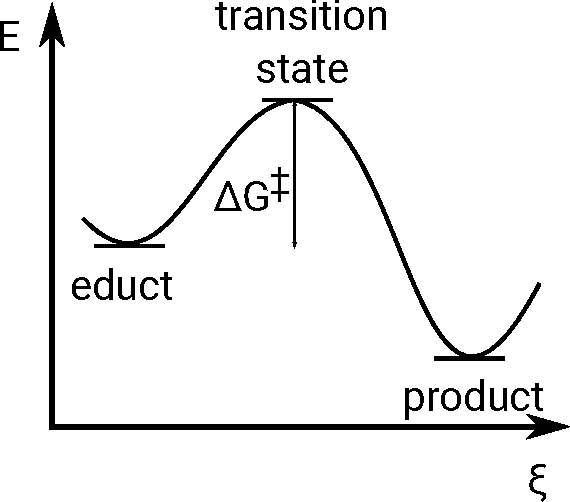
\includegraphics[width=0.4\textwidth]{figures/theory/MEP.pdf}
   \caption{Schematic view of a minimum energy path (MEP) with coordinate $\xi$ for a chemical reaction.
The activation energy $\Delta E^\ddagger= E_\textrm{TS}- E_\textrm{educt}$ for the reaction is also shown.}
            \label{abb:mep}
\end{figure}


% One of the most prominent and widely used theories describing the transition state and the rate constants is Eyring theory of transition states.
% The most important approximations that are made are the following: i) there is an activated complex, ii) all particles that reached this complex/transition state will react towards the product.
% iii) At the transition state geometry, the motion along the reaction coordinate is seen as a one dimensional process and can be separated from all other degrees of freedom and can be seen as a translation.
% \\
% The equation for the rate constant is described by
% \begin{equation}\label{eyring}
% k(T)=\kappa\frac{k_BT}{h}e^{\Delta G^\ddagger(T)/(k_BT)},
% \end{equation}
% with the reaction rate constant $k$, Boltzmann's constant $K_B$, the temperature $T$, the difference of Gibbs free energy for the transition state and the educt $\Delta G^\ddagger$ and the transmission coefficient $\kappa$ that is a transmission coefficient (can be interpreted as a tunneling prefactor, for $\kappa>1$ tunneling occurs and for $\kappa<1$ non-classical reflection) tunneling corrections (seldomly applied in this work, not mention them here?), give the reaction rate constant as a function of temperature and barrier height.
% For the latter one needs to find the energies of the transition state and the educt.
% The educt geometry can simply be obtained by geometry optimization as a minimum on the PES.
% To find the transition state geometry and henceforth the energy we used Nudged Elastic Band calculations (NEB), with Climbing Image, Reaction path is approximated as a series of associated images, which are connected via spring forces.
% These spring forces prevent the images from optimizing into the local minimum next to the transition state.
% First a regular NEB, then on top of this climbing image was done which gives better convergence.
% In this calculation the energetically highest image is "optimized" towards higher energies in the contrary direction of the gradient.For the point found by this scheme we checked whether this is a transition state via frequency analysis, since a TST of first order has to have one imaginary mode that vibrates along the reaction path.

Transition state theory is a semi-classical theory: dynamics along the reaction coordinate $\xi$ are treated classically, but perpendicular modes are treated quantum mechanically in harmonic approximation.


Once a transition state is found (see below), $\Delta E^\ddagger$ and also the corresponding activation free energy
\begin{equation}
\Delta G^\ddagger = G_{TS} - G_{educt}
\end{equation}
can be computed, where $G=H-TS$. %\approx E_{SCF} + G_{vib}$.
The free energy $G$ is a sum of the components for translation, rotation and vibration: $G_{trans}+G_{rot}+G_{vib}$, where only the latter is non zero for reactions studied in this work, where educts and transition state species are adsorbed at a surface.
It can also be expressed by the sum of the SCF energy ($E_{SCF}$) and the vibrational component of the Gibbs free energy using the vibrational frequencies $\nu_i$ from a normal mode analysis:
\begin{equation}
G=E_{SCF} + G_{vib}=E_{SCF}+ \sum_{i=1}^{N_A}\left(\frac{h\nu_i}{2} + k_BT\ln(1-e^{-h\nu_i/(k_BT)})\right).
\end{equation}

With $\Delta G^\ddagger$, reaction rates $k(T)$ can be calculated with the help of transition state theory, according to Eyring\cite{eyring,eyring-polanyi}:
%In thermodynamic equilibrium, all possible quantum states along the reaction coordinate are occupied with respect to their relative Boltzmann weight $P=e^{-\Delta E/(k_BT)}$ depending on the energy $E$ (or free energy $G$) and the temperature $T$.
%Assuming the reaction
%\begin{equation}
%A+ B \rightleftarrows C^\ddagger \rightarrow D
%\end{equation}
%where reactants $A$ and $B$ are in thermodynamical equilibrium with the transition state $C^\ddagger$ and from this the reaction goes to the product $D$.
%The rate constant can be determined with Eyring theory\cite{eyring,eyring-polanyi}:
\begin{equation}\label{eq:eyring}
k(T)=\kappa\frac{k_BT}{h}e^{-\Delta G^\ddagger(T)/(k_BT)}.
\end{equation}
Here, $\kappa$ is a correction factor (accounting for, \textit{e.g.}, tunneling), which we won't use here. $k_B$ is Boltzmann's constant $k_B$.
The equation gives the reaction rate constant as a function of temperature.
Note that this equation is only valid for cases where all reactants reaching the TS react to the product site.
No re-crossing is employed, so the rate is an upper limit in the classical picture.
%For quantum effects, the rate can be increased due to tunneling, where reactants can overcome the barrier although they do not possess sufficient amount of energy for the barrier.
%In order to account for this, the Eyring equation can be expanded with the transmission coefficient $\kappa$ which can be interpreted as a tunneling prefactor.
%For $\kappa>1$ tunneling occurs and for $\kappa<1$ non-classical reflection or re-crossing to the educt side takes place.
\\

For the barrier height one needs to find the free energies of the transition state and the educt.
The educt geometry can simply be obtained by geometry optimization as a minimum on the PES.
Among different methods to find the transition state geometry, we used nudged elastic band calculations (NEB)\cite{Henkelman00a}, with climbing image\cite{Henkelman00b}.
This method approximates the reaction path as a series of associated images, which are connected via spring forces.
These spring forces prevent the images from optimizing into the local minimum next to the transition state.
First a regular NEB, then on top of this climbing image was applied which gives better convergence.
In NEB calculations the energetically highest image is ``optimized'' towards higher energies in the opposite direction of the potential gradient.
Any point found by this scheme must be checked whether it is a transition state via frequency analysis, since a TS of first order has to have one imaginary mode that vibrates along the reaction path.
Otherwise there is no transition state.

\section{Software and Computational Details}
The majority of computations in this work were carried out using the Vienna \textit{ab initio} simulation package (VASP version 4 and 5.2)\cite{kresse1993,kresse2,kresse3,kresse4,kresse99}, which makes use of a plane wave basis.
With VASP we did stationary, periodic DFT calculations and AIMD for a slab model.


For all the VASP calculations with the (0001) surface the parameters from prior work\cite{WirthJPCC2012,Wirth2014,Wirth2015,Wirth2016} were used.
Total energy convergence was achieved when energies between two SCF steps were smaller than $10^{-5}\,$eV, structures were assumed minima if the change in forces between two structures was below $0.01\,$eV/\AA{} and if all frequencies are real.
The energy cutoff was set to $400\,$eV.
A vacuum gap of $26.4\,$\AA{} was used.


These convergence parameters were also adopted for the (11\=20) surface.
Here, the vacuum gap ranged from $17\,$\AA{} for the 10 layer slab to $11\,$\AA{} for the 25 layer slab, depending on the slab size in z-direction.
(For the different slab models used for (11\=20), see Section \ref{sec:11-20}).
%the vacuum region is in the range of 17 Å for the 10 layer slab, 15 for the 15 layer slab, 13 for the 20 layer slab and 11 for the 25 layer slab
\\\\

DFT (PBE and B3LYP) calculations were also done with the program CRYSTAL\cite{crystal14} (version 14), using a real-space representation.
The same program was used for periodic HF calculations.
Further, we performed LMP2 calculations with CRYSCOR\cite{cryscor}.
Both use atom centered bases instead of plane waves.
In all cases, no 3D slabs were calculated but 2D supercells were considered, treating only x and y directions periodically.
Both programs were not applied in our group before so no convergence test had been done so far.
The geometries and cell parameters from the VASP (PBE+D2) output were used as starting points and the usual convergence criteria of the programs were applied, convergence for SCF was achieved when energies between two steps were smaller than $2.7\times 10^{-6}\,$eV (with some exceptions when convergence was hard to achieve).
\\\\

%Energy and plots for the MD shown in this work were prepared with gnuplot\cite{gnuplot}, surface structures and geometries were visualized with VMD\cite{vmd} and further illustrations were created with inkscape\cite{inkscape}.


\chapter{Water on $\upalpha$-Al$_2$O$_3$(0001)}\label{sec:0001}
As mentioned earlier, the (0001) surface is the most stable surface site of alumina under UHV conditions, and it was subject of several studies so far\cite{kuri10,hass98,hass00,Elam1998,Brown1999,Kelber2007,Tsyganenko1996,Chang1971,Lee1985,Nelson1998,Ranea2009,Thissen2009,Shapovalov2000,Wittbrodt1998,Wang2011}.
Both experimental and theoretical studies discovered characteristics and specialties of this crystal cut.
Experimentally, a whole zoo of methods was applied to study the (0001) surface, among which IR\cite{Tsyganenko1996}, LEED\cite{Chang1971} and TEM\cite{Lee1985} studies contributed to characterize the structure of the clean surface and of the latter in contact with water.
Laser-induced thermal desorption spectroscopy\cite{Elam1998,Nelson1998} showed that H$_2$O adsorbs dissociatively on the surface with a variety of hydroxyl surface sites with different binding energies.
Theoretical studies were conducted by means of periodic \textit{ab initio} calculations by Kurita\cite{kuri10} who studied the stability of distinct surface cuts without water. Also the system in contact with H$_2$O was studied by Hass and coworkers\cite{hass98,hass00} with \textit{ab initio} molecular dynamics and they found that dissociation of molecular water is favored.
Several studies found, that water adsorption is preferred at aluminum sites of the Al-terminated surface\cite{hass00,Ranea2009}, but dissociation is energetically more stable than molecular adsorption.
Dissociation creates two distinct OH groups, the so-called OH$_\textrm{ads}$ (adsorbed OH fragment) and OH$_\textrm{surf}$ (OH from surface O and dissociated H atom)\cite{Thissen2009,Ranea2009}.
Further, vibrational frequencies were calculated and compared to experiment\cite{Wirth2014,Wang2011}, and also reaction rates for the dissociation were evaluated\cite{WirthJPCC2012,Wang2011}.
Also cluster studies were conducted approving the findings with periodic models\cite{Wittbrodt1998,Shapovalov2000}.


In our workgroup previous work concerned the adsorption, reactions and vibrational spectroscopy of water on $\upalpha$-Al$_2$O$_3$(0001) in the low-coverage limit.
Furthermore, higher water coverages and hydroxylated surface systems were studied\cite{WirthJPCC2012,Wirth2014,Wirth2015,Melani2018}.
\\

In these studies, periodic DFT in the generalized gradient approximation was used.
It is known (from other systems) that this may lead to errors in computed vibrational frequencies and, notably, in reaction barriers - the latter being typically too low with DFT-GGA.
Further, in none of the studies on Al$_2$O$_3$(0001) the water dosing of the surface with a molecular beam, as used by our experimental partners at the Fritz-Haber Institute, was studied.
In this work, the focus is therefore on two topics:
\\
(i) The testing of methods beyond DFT with GGA functionals (as PBE) for adsorption energies, vibrational frequencies and activation energies for reactions.
\\
(ii) Understanding the scattering processes of a water being shot at the surface with a molecular beam source with the help of AIMD.
\\\\
First, the surface and the most stable adsorption patterns are introduced (Section \ref{sec_0001surf}), followed by the testing of methods beyond DFT-GGA (Section \ref{crystal_calc}), and the results for the molecular beam scattering\cite{Heiden0001_2018} (Section \ref{sec_0001AIMD}).
	
\section{Supercell Model for the Adsorption of Water}\label{sec_0001surf}

In vacuum, the most stable surface cut of $\upalpha$-Al$_2$O$_3$(0001) is a stoichiometric, Al-terminated one.
In this topmost Al layer, the aluminum atoms are undercoordinated and are referred to as coordinatively unsaturated site (CUS).
%In contrast to the (11\=20) surface that will be studied in Section \todo{ref section 11-20} there exists only one type of Al CUS atom, which acts as a reactive Lewis-acid site.
Also, all oxygen atoms are threefold coordinated. %resulting in a less complex topography than for the higher-indexed surfaces.
We apply here a ($2\times 2$) supercell for the Al-terminated (0001) surface with cell vectors that were optimized from the bulk structure (adopted from previous work of Dr. J. Wirth\cite{WirthJPCC2012}).
The surface slab used in this work consists of nine atomic layers that equal three repeating units perpendicular to the surface of the type Al-O$_3$-Al-Al-O$_3$-Al-Al-O$_3$-Al (for the unit cell), with the top five layers being allowed to relax during optimization and AIMD and the lowest four layers being fixed to bulk values, see Figure \ref{abb:surf_0001}.

\begin{figure}[!ht]
 \centering
\subfigure[(0001), top view]{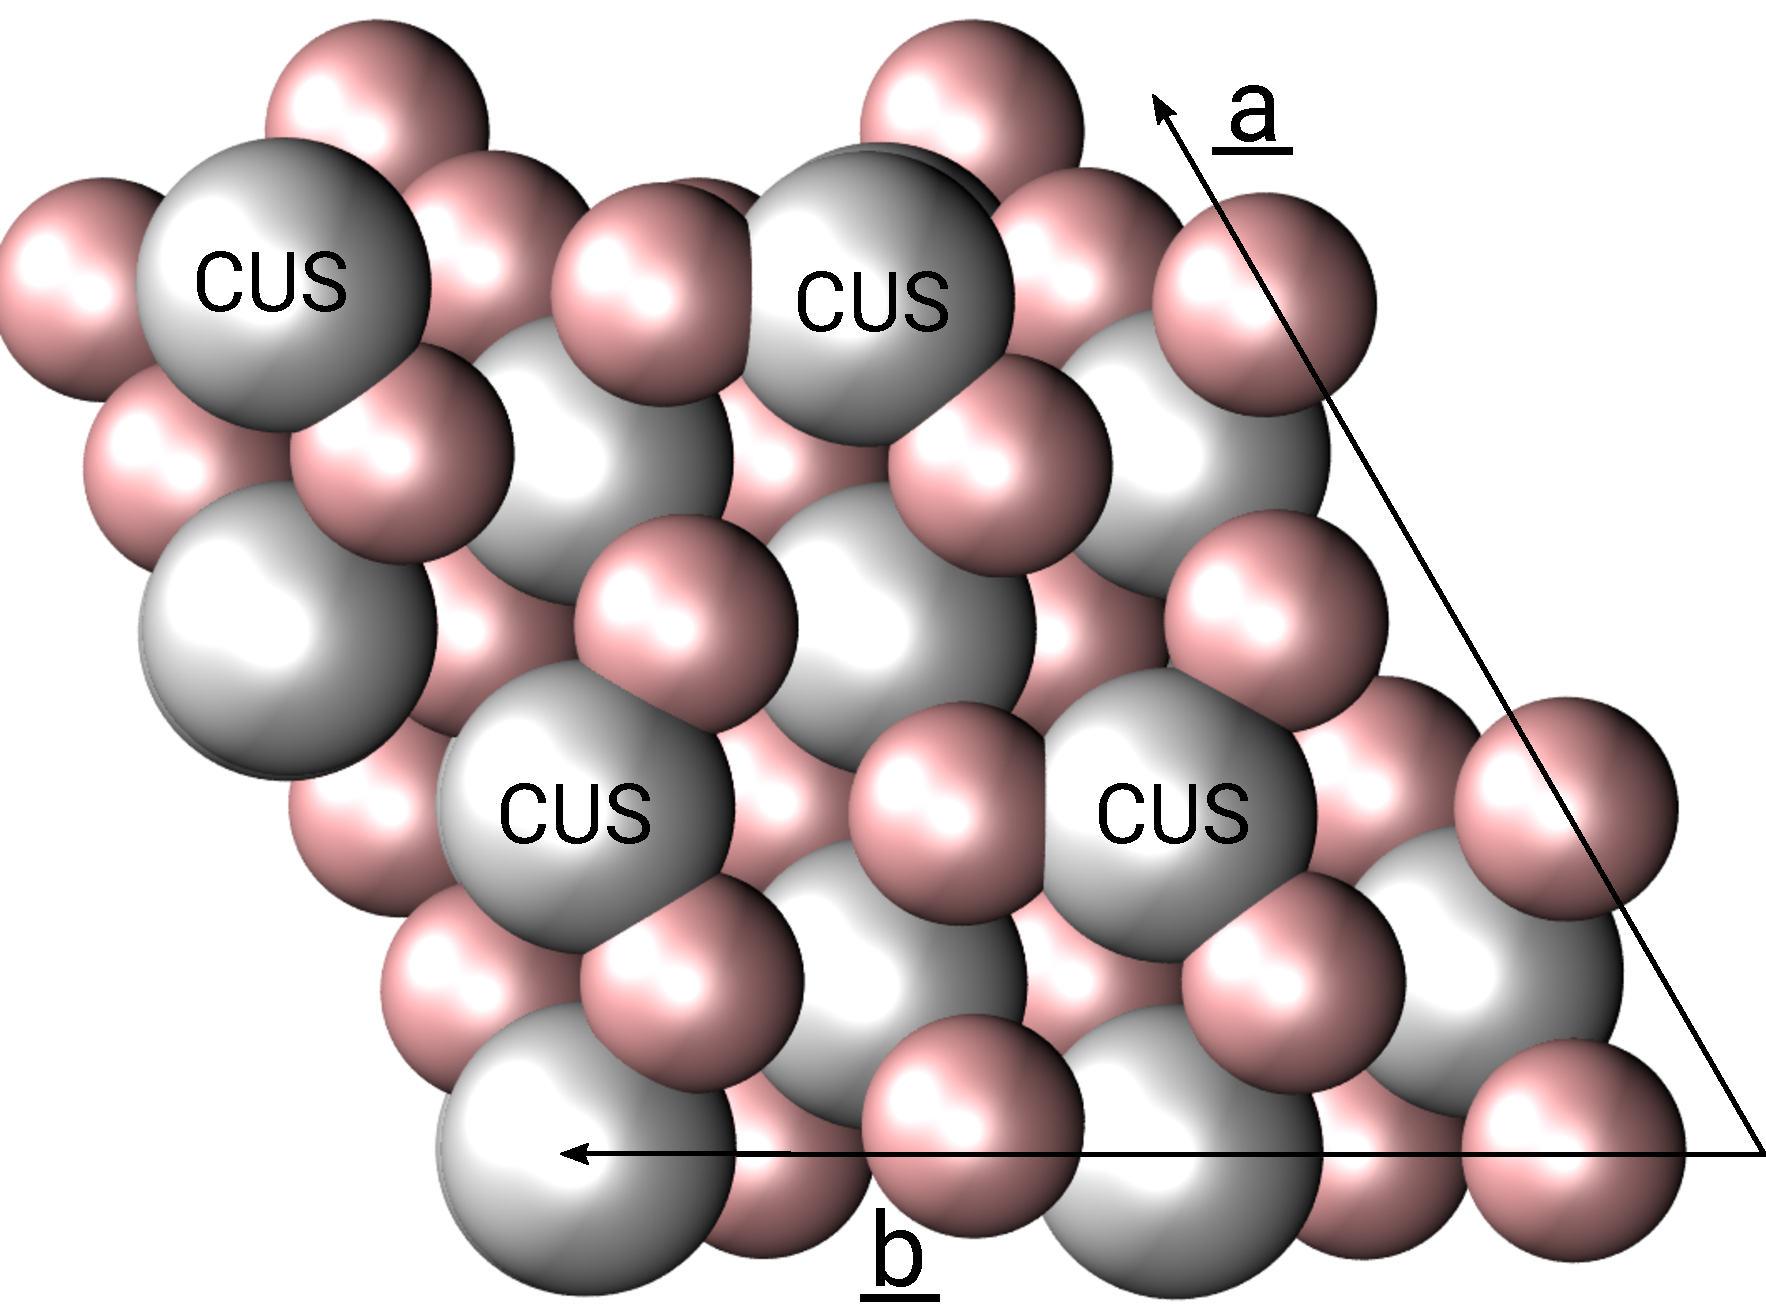
\includegraphics[width=0.4\textwidth]{figures/0001/surf_0K_axes.pdf}}
 \quad\quad
 \subfigure[(0001), side view]{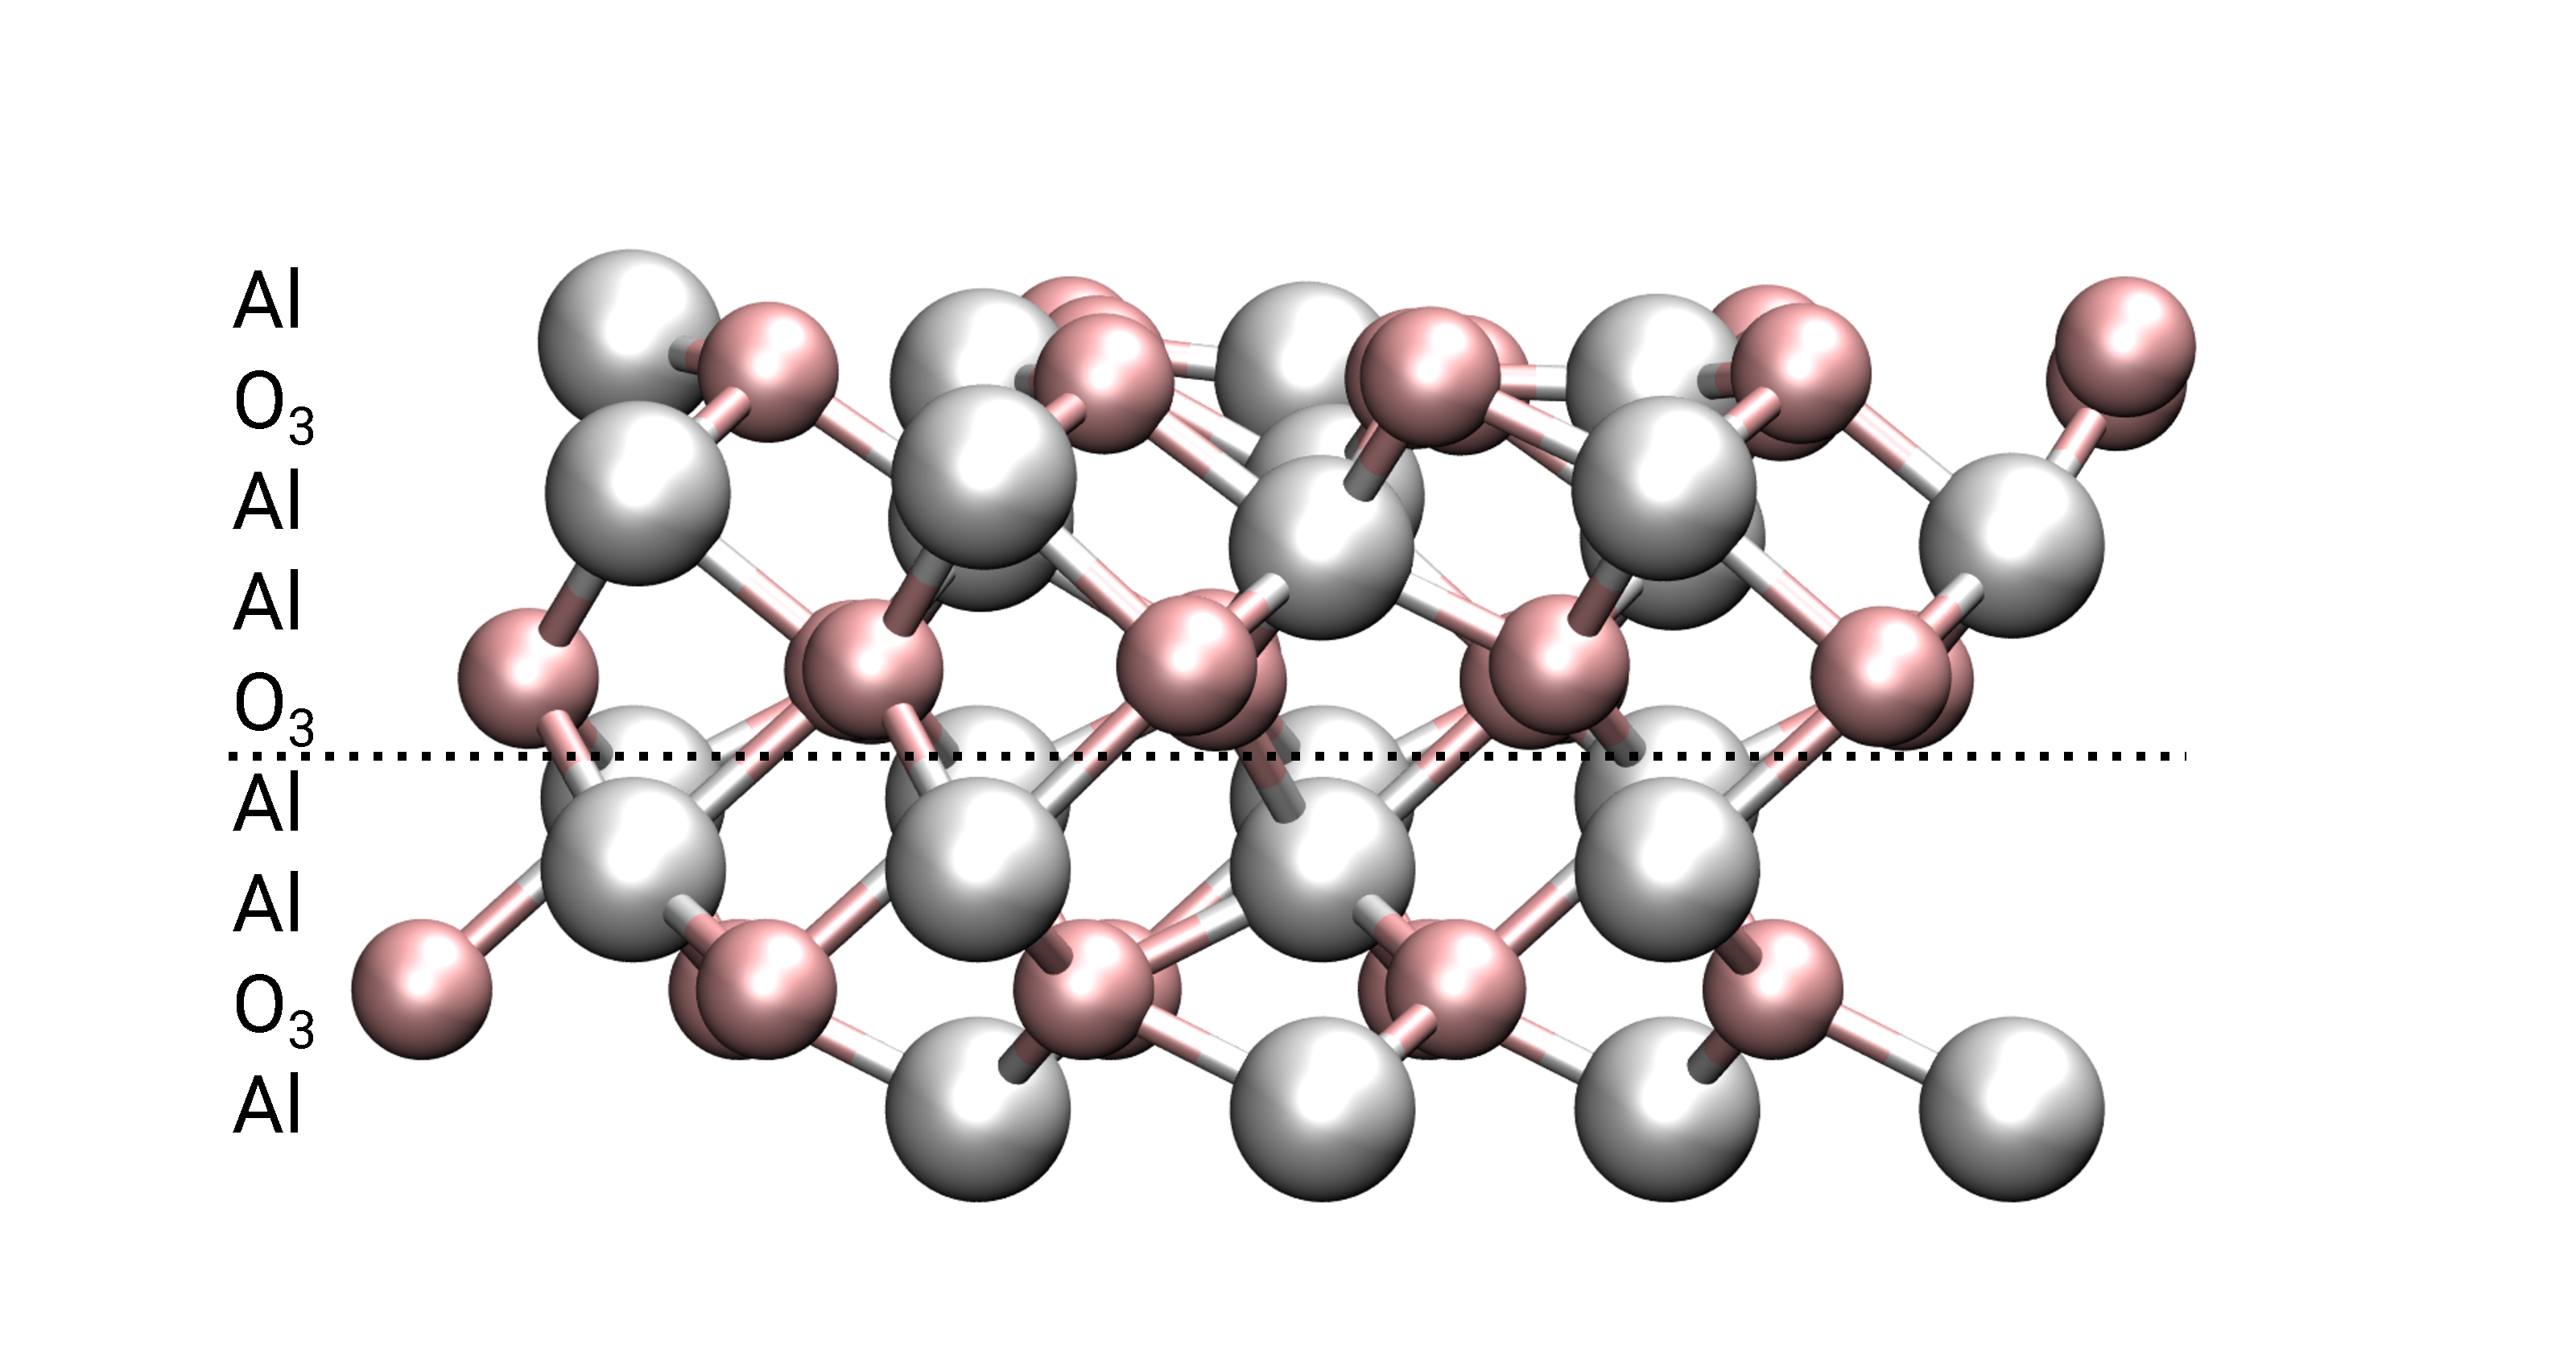
\includegraphics[width=0.45\textwidth]{figures/0001/surf_0K-side.pdf}}
 \caption{Surface model of the (0001), the most stable surface cut under UHV conditions.
The top view (a) shows four Al CUS atoms (gray) for the ($2\times 2$) cell, which are surrounded by three threefold coordinated surface oxygen atoms (pale red).
(b) reveals the side view of the Al-terminated surface cut in detail with the atomic layers indicated.
Atoms below the dashed line are kept fixed to bulk values.}
        \label{abb:surf_0001}
\end{figure}
The unit cell vectors are equal to $|\vec{a}|=|\vec{b}|=9.66\,$\AA  ~and there is a $60$\textdegree{} angle between them.
The $\vec{c}$-vector of the slab model is perpendicular to the plane spanned by $\vec{a}$ and $\vec{b}$ and is $31.4\,$\AA{} long, hence the vacuum gap between two slabs in this direction is $26.4\,$\AA.


The adsorption behavior, vibrations and reactivity of one water  molecule per ($2\times 2$) supercell (coverage 1/4) were already studied in Reference\cite{WirthJPCC2012}.
As mentioned there, there is one molecular minimum on top of a CUS atom and three most stable, dissociated states (see Figure \ref{abb:0001_ads}): the next neighboring 1-2 dissociated state, the 1-4 dissociated structure with the hydrogen atom being one position farther away and the 1-4$^\prime$ that is an example for a species with even greater distance from the OH group.
\begin{figure} [!ht]
\centering
\subfigure[mol]{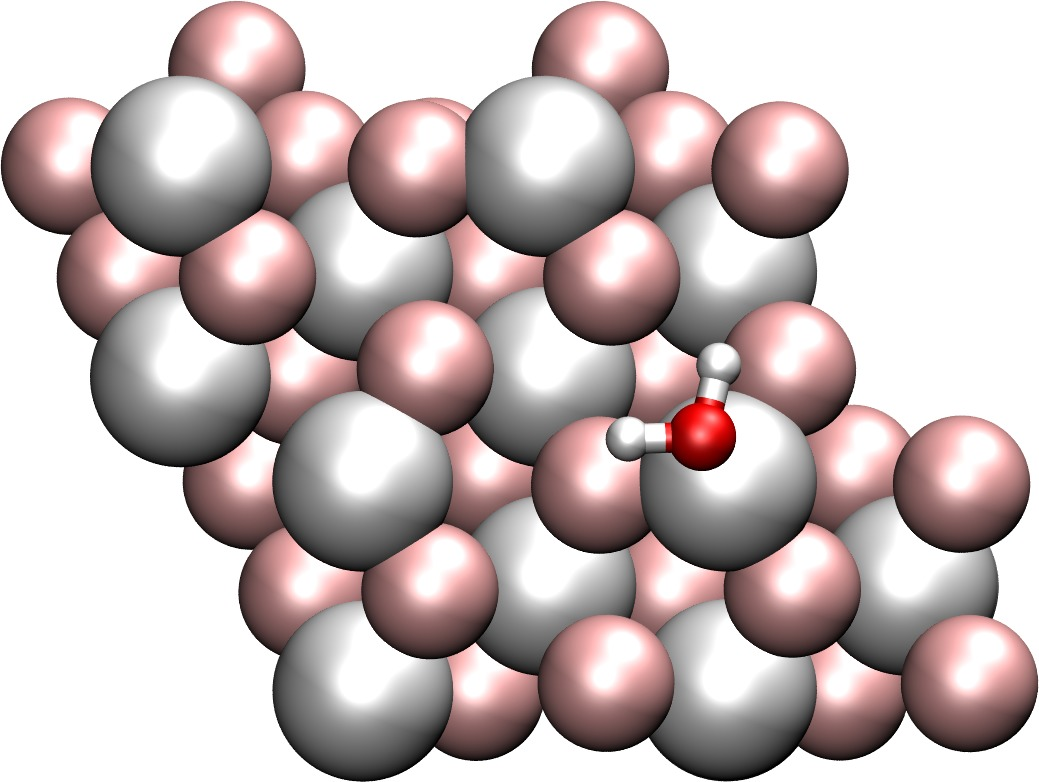
\includegraphics[width=0.4\textwidth]{figures/0001/0001_mol_top.jpg}}
         \quad
\subfigure[1-2]{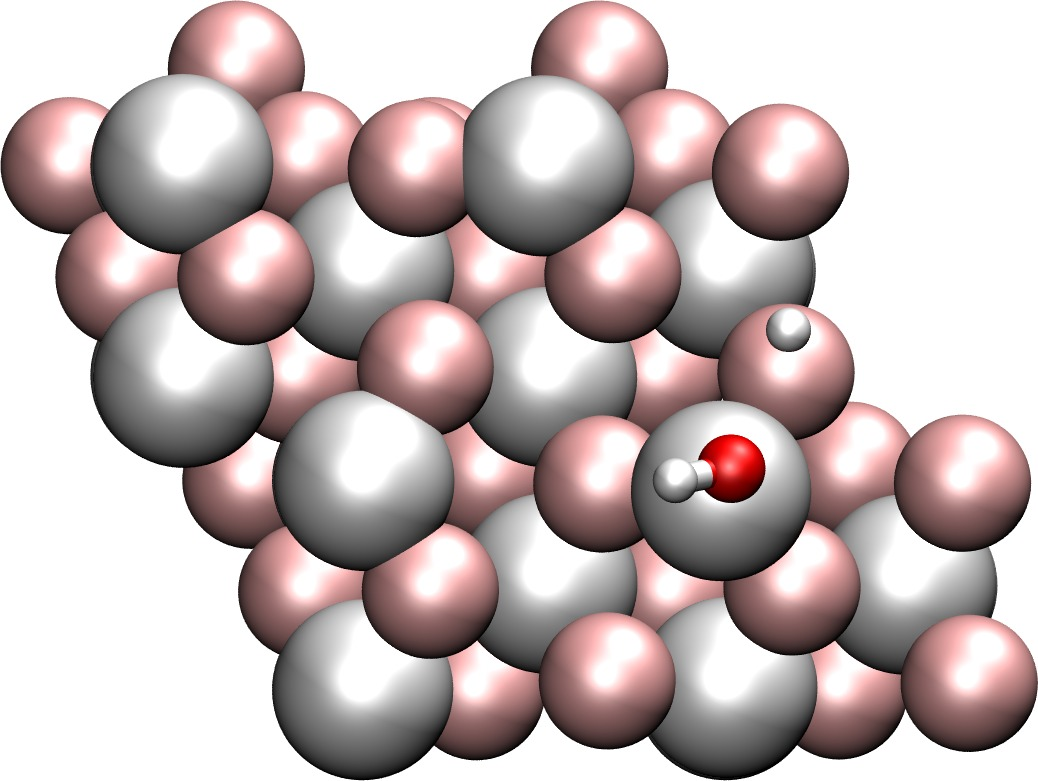
\includegraphics[width=.4\textwidth]{figures/0001/0001_1-2-diss_top.jpg}}
 \quad
\subfigure[1-4]{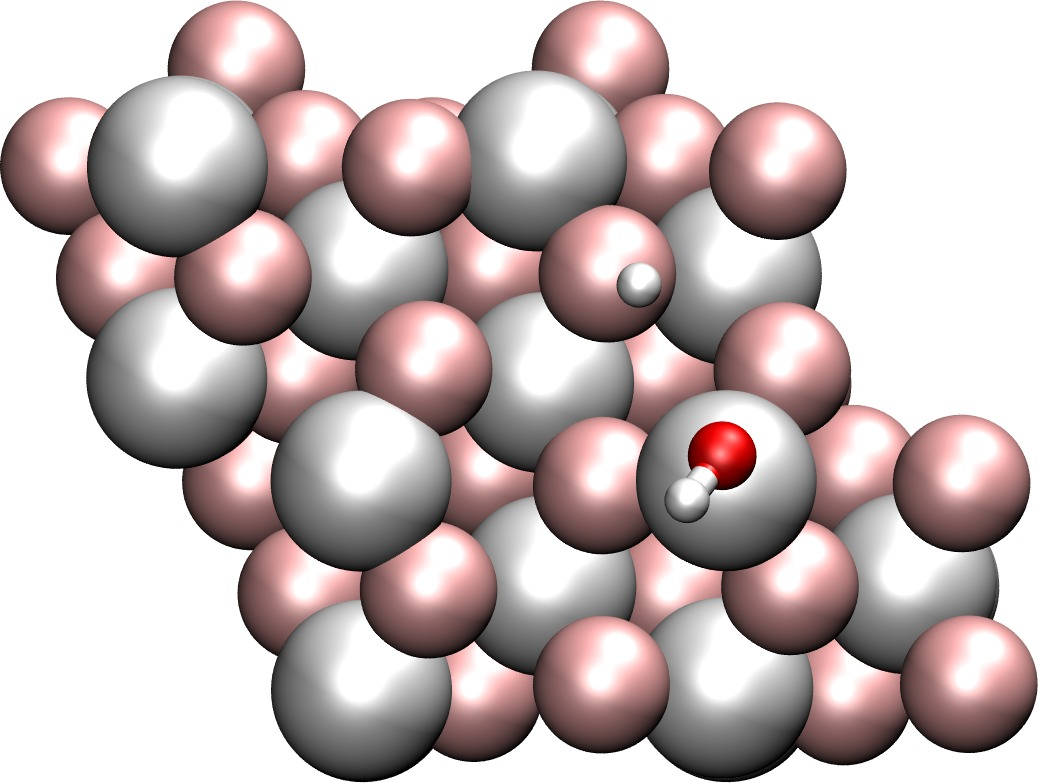
\includegraphics[width=.4\textwidth]{figures/0001/0001_1-4-diss_top.jpg}}
 \quad
\subfigure[1-4$^\prime$]{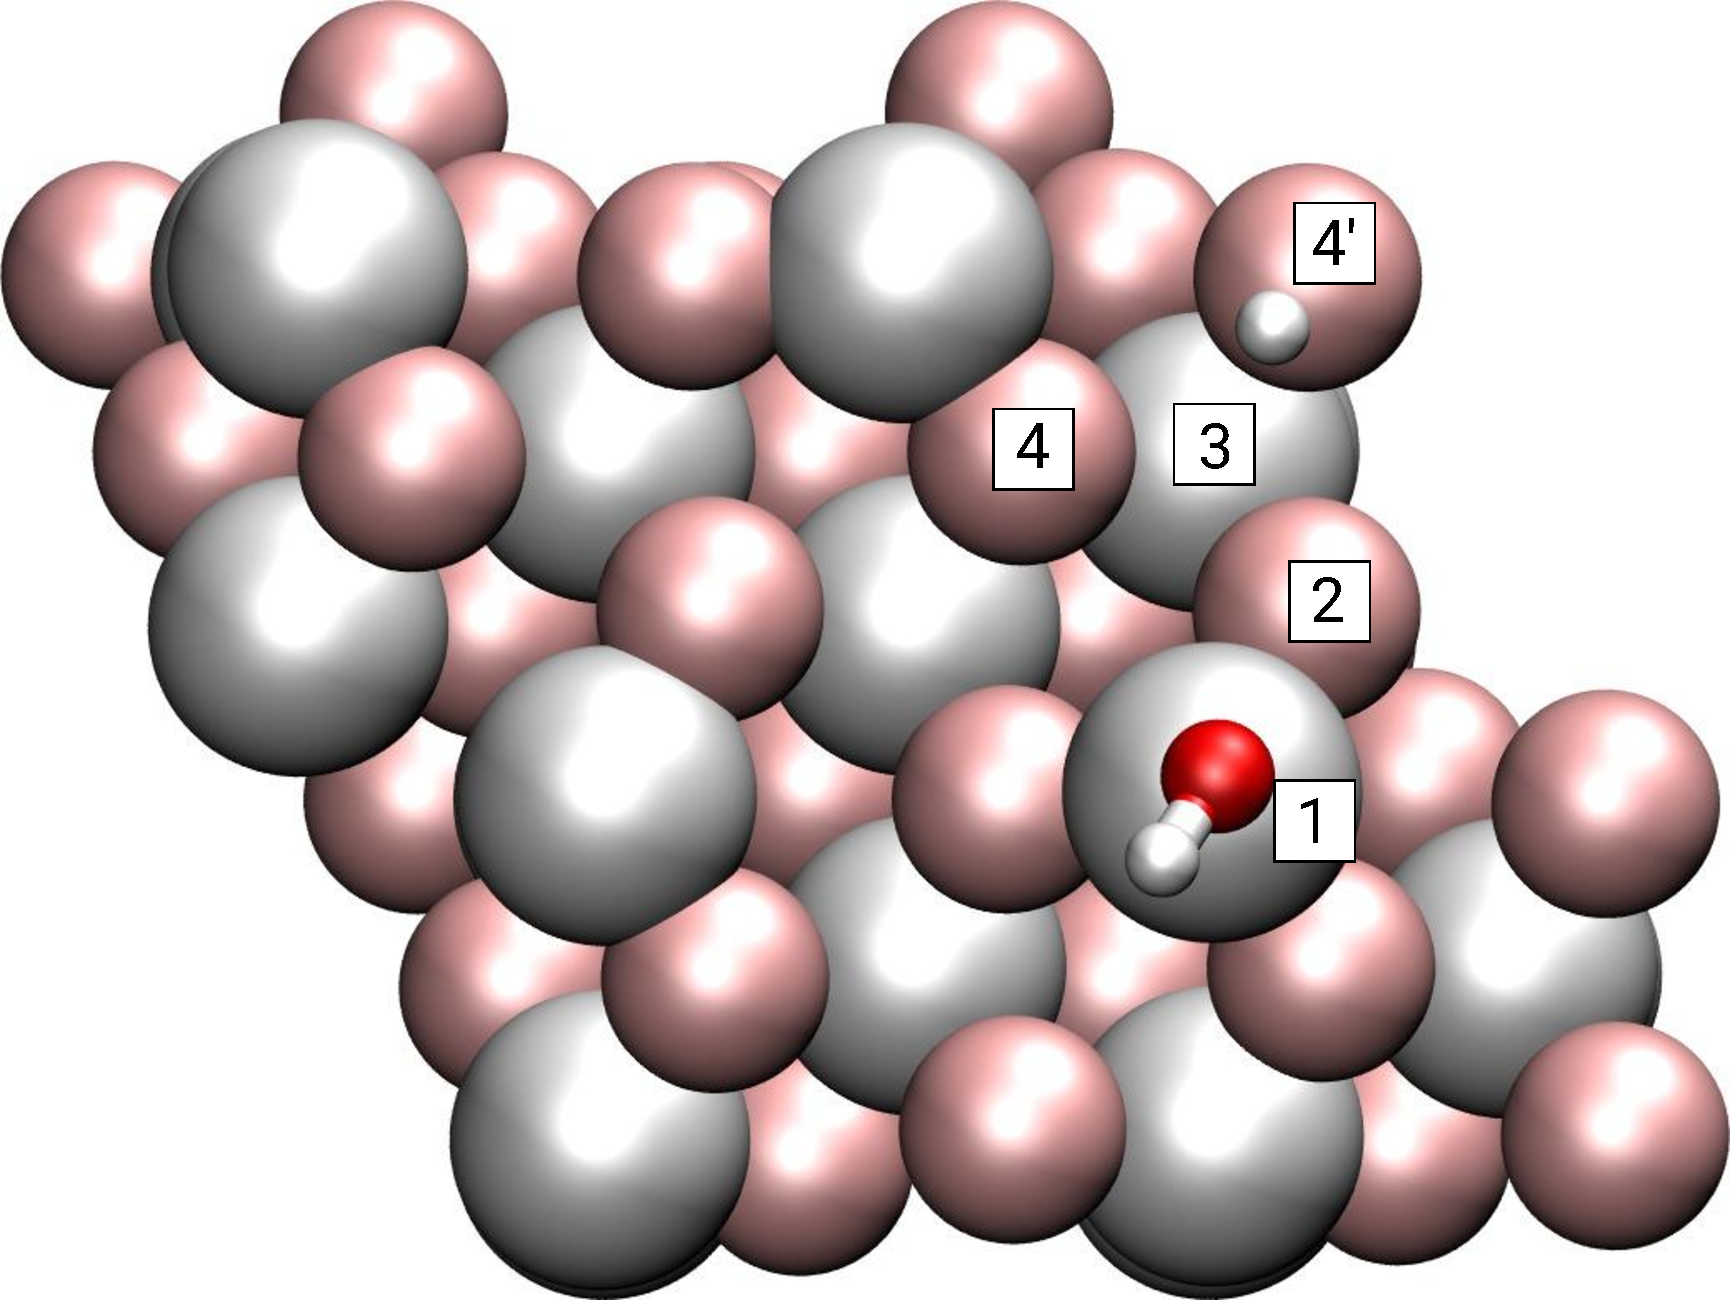
\includegraphics[width=.4\textwidth]{figures/0001/0001_1-4p-diss_top_label.pdf}}
\caption{Adsorption geometries for the plane wave PBE+D2 optimized geometries of the molecular and the three dissociated species.
Additionally, panel (d) shows the numbering of the surface atoms that provides the nomenclature.
Adsorption energies are given in Table \ref{tab:vasp-results}.
The adsorption energy of 1-4$^\prime$ is not listed there and is $E_\textrm{ads}=1.21\,$eV for PBE+D2.
These figures are from unpublished work of Dr. J. Wirth.}
       \label{abb:0001_ads}
\end{figure}
Of these, according to periodic DFT calculations of Reference\cite{WirthJPCC2012} using a plane wave basis and the PW91 exchange-correlation functional, the 1-2 dissociated species is the most stable one and the 1-4$^\prime$ is the least stable one, see Table \ref{tab:vasp-results} below.

The adsorption energy is defined as follows:
\begin{equation}\label{eq:Eads1}
  E_\textrm{ads}=E_\textrm{ads. species}-(E_\text{free water molecule}+E_\text{surface}).
\end{equation}
For the stability of the molecular and the 1-4 dissociated species, the situation is more controversial in the literature\cite{WirthJPCC2012,hass00,Ranea2009}.
In Reference\cite{WirthJPCC2012} PW91 with dispersion corrections gives almost the same adsorption energy for both species.

%In periodic DFT studies with VASP, the stability lies between the previously mentioned ones, depending on the exact method employed: For PBE+D2 the molecular adsorbed species is more stable than 1-4, for the functional PW91+D2 the 1-4 dissociated is more stable, whereas PW91 without dispersion corrections gives the same adsorption energy for both species (the values for the adsorption energy are calculated analogously to the (11\=20) surface cut, equation (\ref{eq:Eads})).
We shall see below (Section \ref{crystal_calc}) that the relative stability of the molecular and the various dissociated species, depends somewhat on the functional, on the treatment (or lack) of dispersion, on the basis (plane wave vs. atomic orbital basis), and on the level of electronic structure method (DFT vs. WFT).
Further, the influence of these methods/basis sets on vibrational frequencies will be studied in Section \ref{sec:AO_freq0001}.
%Calculations with an atom centered basis instead of plane waves with the CRYSTAL code show that the molecular species is more stable for most basis sets and they are both equal in adsorption energy for the remaining ones, see Section \ref{crystal_calc}.


In Reference\cite{WirthJPCC2012}, also reactions linking these minima were studied: dissociation of adsorbed water, OH- and H-diffusion on the surface, as well as rotation of an OH group and molecular water diffusion from one CUS site to another CUS site.
To study the influence of the method/basis set on reaction barriers and rates (the latter obtained by Eyring's transition state theory in Section \ref{crystal-rate}), we will exemplarily refer to the hydrogen diffusion from the 1-4 to the 1-2 adsorbed water (called Df-H-4-2 in \cite{WirthJPCC2012} and here).
The corresponding reaction path (obtained from a NEB calculation in \cite{WirthJPCC2012}) is shown in Figure \ref{abb:df-h-4-2} below.
\begin{figure}[h]
\centering
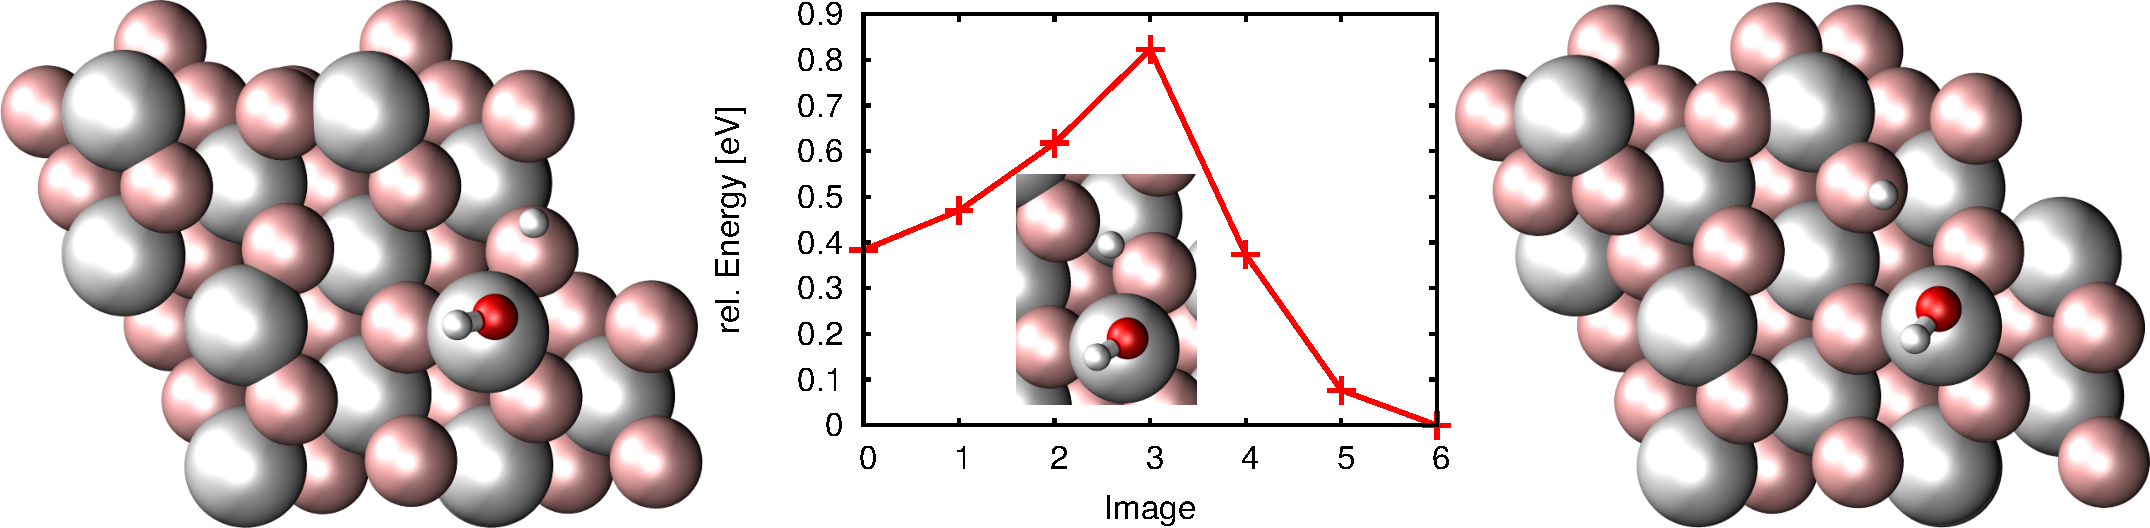
\includegraphics[width=0.98\textwidth]{figures/0001/NEB-path/df-h-4-2.pdf}
\caption{Reaction path of the Df-H-4-2 proton diffusion reaction obtained on the PBE+D2 level of theory via a NEB calculation (middle panel, the inset there shows the transition state), the left panel shows the educt  (the 1-4 dissociated species), and on the right the product species (1-2).
\textit{Unpublished data by Jonas Wirth, with friendly permission}.}
       \label{abb:df-h-4-2}
\end{figure}
%The latter two do not play a crucial role in this work, especially the CUS to CUS diffusion of molecular water is very improbable due to the slow reaction rate.
%Adsorption energies and reaction rates which are of importance for this work are shown in Table \ref{tab:0001_eads} and \ref{tab:0001_rates} (the PBE results shown there are unpublished work obtained by Dr. J. Wirth).
%\begin{table}[!h]
%  \centering
%   \caption{Adsorption energies for the stable minima in eV.
%All values were calculated with PBE including D2 dispersion corrections by Dr. J. Wirth (unpublished).}
%  \begin{tabular}{cccc}
%  \toprule
%   \multicolumn{4}{c}{E$_\textrm{ads}$ [eV]}\\\midrule
%  mol &1-2 &1-4 &1-4$^\prime$  \\
%  -1.31 & -1.69 & -1.30 & -1.21\\\bottomrule
%    \end{tabular}
%  \label{tab:0001_eads}
%\end{table}
%\begin{table}[!h]
%  \centering
%   \caption{Reaction rate constants $k$ in s$^{-1}$ at $300\,$K with corresponding barrier heigths $\Delta E^\ddagger$ and $\Delta G^\ddagger_\textrm{300\,K}$ in eV for the processes connecting the minima.
%Calculations were executed with PBE+D2 (also from unpublished work of Dr. J. Wirth).}
%  \begin{tabular}{c|ccc||ccc}
%  \toprule
%   &\multicolumn{3}{c}{reaction} & \multicolumn{3}{c}{back reaction}\\
%   &              $\Delta E^\ddagger$ & $\Delta G^\ddagger(\textrm{300\,K})$ &%$k(\textrm{300\,K})$&$\Delta E^\ddagger$ & $\Delta G^\ddagger(\textrm{300\,K})$ %&$k(\textrm{300\,K})$\\\midrule
%diss-1-2         &0.13 & 0.11 & 8.0$\times 10^{10}$ & 0.50 & 0.50 & 2.3$\times 10^4$ \\
%diss-1-4         &0.19 & 0.14 & 2.8$\times 10^{10}$ & 0.19 & 0.14 & 2.7$\times 10^{10}$\\
%diff-2-4         &0.82 & 0.68 & 2.7$\times 10^1$ & 0.44 & 0.29 & 9.1$\times 10^7$ \\
%diff-2-4$^\prime$&0.81 & 0.67 & 3.8$\times 10^1$ & 0.33 & 0.20 & 3.1$\times 10^9$\\
%diff-4-4$^\prime$&0.61 & 0.41 & 7.1$\times 10^5$ & 0.51 & 0.33 & 1.7$\times 10^7$\\\bottomrule
%    \end{tabular}
%  \label{tab:0001_rates}
%\end{table}
%\\

%The desorption process from the surface itself was studied by starting from the molecular minimum, gradually doing optimizations with greater O-surface distance and letting everything relax except for the c coordinate of the water-oxygen atom.
%This calculations give an energy profile for the adsorption/desorption but no barrier could be found (see Figure \ref{abb:0001_desorption}), so the underlying adsorption process is assumed to be barrierless.
%  \begin{figure}[!ht]
%   \centering
%   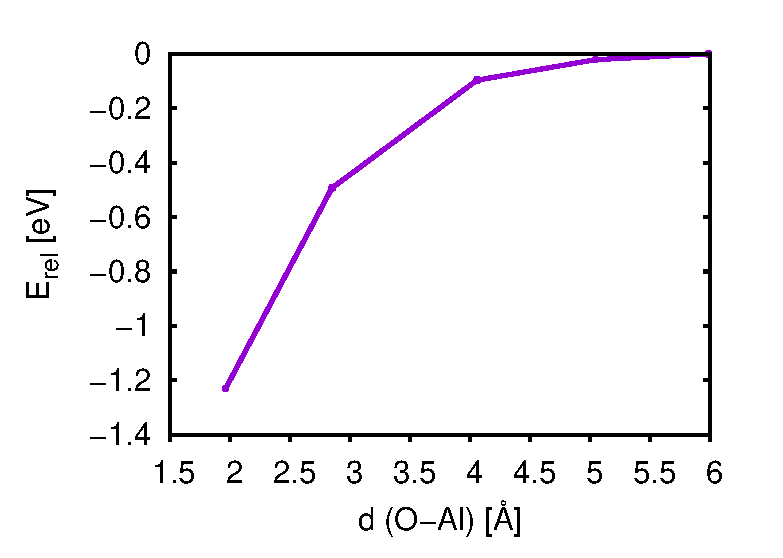
\includegraphics[width=0.45\textwidth]{figures/0001/mol_ads_barrier.eps}
%   \caption{Energy profile of the adsorption process, relative to the energy of the system with a distance of $5.98\,$\AA.
%d(O-Al) denotes the distance between the oxygen atom of the water and the Al CUS where the water is/was adsorbed molecularly.
%%/und/sophia/0001_mol_ads_barrier/
%   }
%   \label{abb:0001_desorption}
%  \end{figure}
%\\
%%%%%%%%%%%%%%%%%%%%%%%%%%%%%%%%%%%%%%%%%%%%%%%%%%%%%%%%%%%%%%%%%%%%%%%%%%%%%%%%%%%%%%%%%%%%%%%%%%%%%%%%%%%%%%%%%%%%%%%%%%%%%%
\section[Adsorption Energies, Vibrations and Reactions of Water on $\upalpha$-Al$_2$O$_3$(0001)]{Adsorption Energies, Vibrations and Reactions of Water on $\upalpha$-Al$_2$O$_3$(0001) with and beyond DFT-GGA}\label{crystal_calc}
As stated in the introduction, GGA functionals deliver poor barrier heights and reaction rates.
In order to improve reaction rates with a high-level method, we chose the hydrogen diffusion reaction DF-H-4-2 as indicated in Figure \ref{abb:df-h-4-2}.
% a model reaction.
%This reaction is a H-diffusion reaction on the (0001) surface studied before in our group, the Df-H-4-2 reaction\cite{WirthJPCC2012} that moves a proton in the 1-4 position to the OH residue to the 1-2 dissociated state (see Figure \ref{abb:df-h-4-2}).
There, the transition state was calculated with PBE+D2 with the implementation of nudged elastic band in VASP using a plane wave basis.
Rates were calculated via Eyring transition state theory (Equation (\ref{eq:eyring})).

%A further previous approach involving single point calculations at the HSE level of theory (hybrid functional) on top of PBE optimized geometries was analyzed for the minima and the transition state.
%Additionally, for this process a 1-D potential energy surface was calculated and then the Schrödinger equation was solved to obtain the wave function and see the localization/delocalization along the reaction pathway.
%These results are summarized in Table \ref{tab:4-2results_jonas}.
% \begin{table}[!h]
%   \centering
%   \caption{PW91, PBE+D2 after geometry optimization and transition state via NEB, HSE single point calculations on top of PBE optimized geometries.
% Both were calculated from Eyring equation (\ref{eq:eyring}).
% The exact tunneling was calculated from a 1-D potential and the calculation of the Schrödinger equation in this potential.
% These calculations were conducted by Dr. J. Wirth and are partially unpublished.}
% \hspace*{-1cm}
%  \begin{tabular}{l|cc}
%  \toprule
%  Method&$\Delta G^\ddagger$ [eV]&k [s$^{-1}$] \\
%     \midrule
%  PW91 & 0.27& $1.97\times 10^8$\\
%  PBE+D2 & 0.29&$9.15\times 10^7$\\
%  %HSE & &$3.15\times 10^7$\\
%  %``exact'' tunneling (1D) & &$6.49\times 10^8$\\
%  \bottomrule
%   \end{tabular}
%   \label{tab:4-2results_jonas}
% \end{table}


It is now our goal to test the accuracy of gradient-corrected DFT using, plane wave bases, against alternative methods/approaches.
Specifically, the following will be done:
\begin{enumerate}
\item Using VASP, we will first compare various flavors of plane wave, three-dimensional supercell DFT-GGA: PBE+D2, PBE+D3, PW91 and PW91+D2.
\item We will then, using atom centered orbital basis (AO), test the performance of PBE+D3.
This will be done with the CRYSTAL code, using a two-dimensional slab model.
This allows us to test not only basis set effects, but also effects due to the choice of slab vs. supercell models.
\item Using CRYSTAL, 2D slab models and AO bases, we will test a hybrid DFT functional common in molecular chemistry, B3LYP (with dispersion corrections, D3).
\item Finally, we will also test pure wave function methods within 2D-slab/AO models, namely the Hartree-Fock (using CRYSTAL) and local M\o{}ller-Plesset perturbation theory of second order, LMP2 (using CRYSCOR).
\end{enumerate}
We will apply these methods not only for barriers and kinetics, but also for adsorption energies and vibrational frequency analyses.

%expand these methods to the following: by first calculating the adsorption energies and the barrier within an atom centered orbital method with the hybrid functional B3LYP and also going beyond density functional theory by employing perturbation theory (local M\o{}ller Plesset perturbation theory of second order, LMP2).
%After this, the transition state shall be reoptimized with B3LYP and the respective rates shall be calculated for this geometry both with density functional theory (PBE and B3LYP) and LMP2.
%\\
%Apart from that, we study this reaction with the help of Path Integral Molecular Dynamics, where the system is represented as a couple of beads that are connected and henceforth act as a more delocalized particle which can contribute to quantum effects, proton tunneling.
%\\
%As a last approach, we want to apply other higher level methods in an embedded approach.
%We cut a cluster from the surface situation and embed this cluster in a field of point charges.
%By doing this we can calculate the cluster with a better method, let's say B3LYP, CCSD or MP2 and then apply a substractional scheme to get to corrected adsorption energies that can then be used to improve the rates with Eyring's equation for transtition states.

% \subsection{MP2 and B3LYP}
% Going beyond pure density functionals and also beyond DFT has been too costly for a long time, simply not applicable for surface adsorbat system that large and electron rich.
%In the crystal\cite{crystal14}/cryscor\cite{cryscor} code one uses atom centered bases instead of plane waves and so large scale systems can also be computed.
%We first optimized our parameters with HF calculations and then did calculations with PBE similar to prior plane wave based calculations.
% \\
% We found out that BSSE takes a big part, but corrections are not easily applied because the ghosted calculations needed for that do not converge for all the structures with a bigger OH-H distance.
%Instead we have to use bigger basis sets containing diffuse functions in order to handle the BSSE.
%Such a self designed basis set by our cooperation partner Dr. Denis Usvyat (HU Berlin, group of Martin Sch\"utz) was used here.
%With this basis set we did the PBE calculations again (?) and the B3LYP as well as the MP2 calculations.
%First we compared the differences in adsorption energies.
%We furthermore compared the vibrational frequencies from B3LYP with the ones from VASP/PBE to see a methodological effect.
% \\
% We also reoptimized the transition state for the Df-H-4-2 reaction.

\subsection{Adsorption Energies}\label{sec:eads_crystal}
 \subsubsection{GGA-DFT Calculations using PW Bases}
For the GGA-DFT calculations using PW bases and VASP, a $\vec{k}$-point mesh of ($3\times 3\times 1$), an energy cutoff of $400\,$eV and a convergence criterion of $10^{-5}\,$eV was adopted.
In all cases, geometry optimizations for reactants and products were performed with the respective method.

In Table \ref{tab:vasp-results} the adsorption energy of VASP calculations with different functionals (PBE and PW91) with and without dispersion corrections are shown.
The adsorption energy is calculated according to Equation (\ref{eq:Eads1}).
\begin{table}[!h]
  \centering
   \caption{Adsorption energies $E_\textrm{ads}$ (in eV) of the molecular and two dissociated adsorption states of H$_2$O on the alumina(0001) surface, obtained with VASP using a supercell approach and a plane wave basis.}
  \begin{tabular}{l|ccc}%c}
  \toprule
  method & mol & 1-2 diss & 1-4 diss\\\midrule %&1-4$^\prime$ diss\\\midrule
  PW91$^a$   &-1.25 &-1.59 &-1.25 \\%&-\\
  PW91+D2$^a$&-1.40 &-1.81 &-1.45 \\%&-\\
  PBE+D2$^b$ & -1.31 & -1.69 & -1.21 \\
  PBE+D3 &-1.29&-1.63 &-1.30 \\\bottomrule%&-1.25 \\\bottomrule
  \end{tabular}
    \begin{tablenotes}
 \footnotesize
\item[a] $^a$ J. Wirth, Reference \cite{WirthJPCC2012,Wirth2014thesis}
\item[b] $^b$ J. Wirth, unpublished
\end{tablenotes}
  \label{tab:vasp-results}
 \end{table}
\\

The adsorption energy is in favor of the 1-2 dissociated species for all methods.
The next stable species is either the molecular adsorbate of 1-4, depending on the dispersion corrections used, or not, and on functional.
The molecular and 1-4 dissociated species are equally stable (PW91, PBE+D3), or the latter is slightly more stable (PW91+D2), or less stable (PBE+D2).
With dispersion corrections for PW91, all adsorbates get stabilized, but the molecular species is less stabilized than the dissociated adsorbates.
In the case of PBE with dispersion corrections, we see that D2 and D3 do not change the results strongly, and also both stabilization (1-4 is stabilized with D3) and destabilization (mol and 1-2) occur.

 \subsubsection{GGA-DFT Calculations using AO Bases}
We now compare for a particular GGA functional, PBE+D3, the performance of AO bases (and a two-dimensional slab model), to the plane wave results just mentioned.
Calculations are done with the CRYSTAL code.
We use a ($4\times 4 \times 1$) $\vec{k}$-point grid and a convergence criterion for the total energy is $2.7\times 10^{-6}\,$eV.
When employing the CRYSTAL program, we first have to chose suitable basis sets.
The basis sets which were tested are summarized in Table \ref{tab:basissets}.
\begin{table}[!h]
  \centering
   \caption{Applied basis sets for Al, O and H in the CRYSTAL calculations.
   The ordering is according to their size.
   Citations can be found in the table footnotes.
   The basis set names are adopted from the CRYSTAL basis set database.
   Basis sets 8 and 9 are developed further from basis sets in the CRYSTAL basis set data base.
   Further details can be found in Appendix \ref{app_combined_basis}.}
  \begin{tabular}{c|lll}
  \toprule
  basis set & Al & O & H \\\midrule
   1&Al$\_$85-11G$^\ast\_$catti$\_$1994 &O$\_$m-6-311G(d)$\_$Heyd$\_$2005 & H$\_$pob$\_$TZVP$\_$2012\\
   2&Al$\_$86-21G$^\ast\_$harrison$\_$1993 &O$\_$m-6-311G(d)$\_$Heyd$\_$2005 & H$\_$pob$\_$TZVP$\_$2012\\
   3&Al$\_$85-11G$^\ast\_$catti$\_$1994 &O$\_$pob$\_$TZVP$\_$2012 & H$\_$pob$\_$TZVP$\_$2012\\
   4&Al$\_$86-21G$^\ast\_$harrison$\_$1993 &O$\_$pob$\_$TZVP$\_$2012 & H$\_$pob$\_$TZVP$\_$2012\\
   5&Al$\_$s8511p511d11$\_$Heifets$\_$2013 & O$\_$8411(d11)$\_$Heifets\_2013&H$\_$pob$\_$TZVP$\_$2012 \\
   6&Al$\_$m-6-311G(d)$\_$Heyd$\_$2005 &O$\_$m-6-311G(d)$\_$Heyd$\_$2005 & H$\_$pob$\_$TZVP$\_$2012\\
   7&Al$\_$pob$\_$TZVP$\_$2012 &O$\_$pob$\_$TZVP$\_$2012 & H$\_$pob$\_$TZVP$\_$2012\\
   8&\multicolumn{3}{c}{customized, high angular momentum basis} \\
   9&\multicolumn{3}{c}{basis set 8 with dual basis set expansion, adding further diffuse functions}\\\bottomrule
  \end{tabular}
  \begin{tablenotes}
 \footnotesize
\item[Heifets] Heifets: \cite{heifets}, pob$\_$TZVP: \cite{pobTZVP}, Heyd: \cite{heyd1,heyd2}, Catti: \cite{catti}, Harrison: \cite{harrison1,harrison2}
\end{tablenotes}
  \label{tab:basissets}
\end{table}
The basis sets are numbered with increasing size, so that the largest number corresponds to the highest number of basis functions.

Again, in each case, the geometries of H$_2$O, the clean surface and the three adsorbed species (mol, 1-2 and 1-4) were optimized.
The corresponding adsorption energies for PBE+D3 can be found in Table \ref{tab:basisset-results-PBE+D3}.
\begin{table}[!h]
  \centering
   \caption{Adsorption energies $E_\textrm{ads}$ (in eV) from Equation (\ref{eq:Eads1}) for the three considered adsorption states of water on alumina(0001) surface (PBE+D3, geometry optimizations were evaluated with the respective basis set from Table \ref{tab:basissets}).}
  \begin{tabular}{c|ccc}
  \toprule
  basis set & mol & 1-2 diss & 1-4 diss \\\midrule
  1 &-1.87 &-2.11 &-1.75 \\
  2 &-1.74 &-1.96 &-1.58 \\
  3 &-1.53 &-1.78 &-1.43 \\
  4 &-1.58 &-1.73 &-1.40 \\
  5 &-1.57 &-1.77 &-1.38 \\
  6 &-1.72 &-1.96 &-1.59 \\
  7 &-1.47 &-1.69 &-1.35 \\
  8 &-1.41 &-1.68 &-1.32 \\\bottomrule  
  \end{tabular}
  \label{tab:basisset-results-PBE+D3}
\end{table}
\\

All basis sets that were tested predict with PBE+D3 the stability order 1-2 $>$ mol $>$ 1-4.
In contrast the VASP PBE+D3 plane wave calculation predicts an almost equal energy for mol and 1-4 diss.
% The absolute values of adsorption energies are larger than the PW values, which might be due to the basis set superposition error (BSSE).
Most of the absolute values of the adsorption energies are too large when compared to the PBE+D3 values for the plane wave basis, by up to $\sim$0.6$\,$eV.
We attribute these larger values to some extent to basis set superposition errors (BSSE) which occur in AO-based calculations but not when using plane wave bases.
In fact, as shown in Appendix \ref{app:BSSE}, for the case of basis 4, where the BSSE was evaluated, about $10\%$ of the adsorption energy is due to BSSE for this basis.
To overcome this problem, the larger ``customized'' basis set 8 was introduced for which the BSSE is expected to be smaller.
In fact, the PBE+D3/AO absolute adsorption energies shown in Table \ref{tab:basisset-results-PBE+D3} agree with PBE+D3/plane wave to within $0.02\,$eV (for 1-4 diss) to $0.12\,$eV (for mol).
Deviations in the order of $0.1\,$eV are easily expected also due to the (other) computational settings (\textit{e.g.}, 2D slab vs. 3D supercell models).


More important than absolute energies are energy differences between adsorbed species.
Here most AO bases agree with energy differences obtained with PBE+D3/PW within $\sim$0.1-$0.2\,$eV.
For basis set 8, for example, the energy difference between mol and 1-2 diss is $-0.27\,$eV while the PW calculation gives $-0.34\,$eV, and the energy difference between mol and 1-4 diss is $+0.09\,$eV compared to $-0.01\,$eV.

% In addition to adsorption energies from optimized geometries, for basis set 5 adsorption energies were calculated with the previous VASP optimized structure (\textit{i.e.} only single point calculation with CRYSTAL) to compare to VASP results.
% Those results are given in Table \ref{tab:pbe-vasp-geom}.
% \begin{table}[!h]
%   \centering
%    \caption{Adsorption energies of the four adsorption states of the 0001 surface site (PBE+D3 with basis set 5 (see Table \ref{tab:basissets})).
% Values are given in eV.
% VASP values are reoptimized from J. Wirth's work with PBE+D3.}
%   \begin{tabular}{cccc}%c}
%   \toprule
%    &mol & 1-2 diss & 1-4 diss\\\midrule %&1-4$^\prime$ diss \\\hline
% CRYSTAL (opt) & -1.57 & -1.77 &-1.38 \\%&-1.32 \\
%    CRYSTAL (no opt)&-1.67 &-1.87 &-1.52\\%&-1.50 \\
%   VASP &-1.29 &-1.63 &-1.30 \\%&-1.25 \\
%   \bottomrule
%   \end{tabular}
%   \label{tab:pbe-vasp-geom}
% \end{table}
% Both CRYSTAL results (reoptimized and VASP optimized geometry) give qualitatively the same ordering of the stability (mol is more stable than 1-4), which is different to former VASP results, although quantitative differences exist.
% Interestingly, the non optimized system seems more stable which is suprising at first sight.
% Due to different amounts of stabilization in the clean surface, the adsorbed system and the free water molecule, the adsorption energies are stabilized more for the calculations with the VASP optimized geometries than for the CRYSTAL reoptimized ones.
% \\\\
Going beyond pure density functionals and also beyond DFT has been too costly for a long time, and it is simply not applicable for a surface adsorbate system as large and electron rich as ours.
However, in the CRYSTAL14\cite{crystal14} and CRYSCOR\cite{cryscor} codes atom centered bases are used instead of plane waves so that large scale systems can also be computed.
With this methodology it is possible to calculate periodic structures with GGA as well as with hybrid functionals and, moreover, with wave function-based techniques like LMP2.

\subsubsection{Hybrid-DFT Calculations using AO Bases}
Going beyond PBE (GGA functional), the hybrid functional B3LYP including D3 dispersion corrections was applied.
Geometry optimizations were performed and adsorption energies were examined, see Table \ref{tab:basisset-results-B3LYP+D3}.
 \begin{table}[!h]
  \centering
   \caption{Adsorption energies $E_\textrm{ads}$ (in eV) from Equation (\ref{eq:Eads1}) for the three considered adsorption states of water on alumina(0001) surface (B3LYP+D3, AO basis, geometry optimizations were evaluated with the respective basis set from Table \ref{tab:basissets}).
   The basis sets 4, 7 and 8, which are highlighted are used for further calculations.}
  \begin{tabular}{c|ccc}
  \toprule
  basis set & mol & 1-2 diss & 1-4 diss \\\midrule
  1 &-1.90 &-2.25 &-1.83 \\
  2 &-1.80 &-2.14 &-1.69 \\
  3 &-1.62 &-2.01 &-1.62 \\
  \textbf{4} &-1.57 &-1.95 &-1.57 \\
  5 &-1.56 &-1.88 &-1.45 \\
  6 &-1.78 &-2.15 &-1.68 \\
  \textbf{7} &-1.57 &-1.92 &-1.53 \\
  \textbf{8} &-1.43 &-1.81 &-1.40 \\\bottomrule
  \end{tabular}
  \label{tab:basisset-results-B3LYP+D3}
\end{table}
\\
Most basis sets also give the same ordering as PBE+D3, but basis 3 and 4 qualitatively give the same trends as VASP (adsorption energy for mol and 1-4 diss equal, like PW91 and PBE+D3) and also basis set 7 is very close to this.
Henceforth, basis sets 4, 7 and 8 are used in further calculations; for the more computationally demanding transition state optimization the smaller basis 4 is used, for normal mode analyses, basis set 7 is used and basis 8 for adsorption energies.



% 
% Since it was not possible to calculate the BSSE and respective relaxation and interaction energies for the 1-4 dissociated system, it is necessary to go on using an extended basis instead, to get (hopefully) the same effect as with CP corrections.
% This larger basis set is a customized triple zeta basis set with high angular momentum (see Appendix \ref{app_combined_basis}).
\clearpage
\subsubsection{Wave Function Theory with AO Basis}

% As before, geometry optimizations were realized and the adsorption energies were evaluated, as shown in Table \ref{tab:combined_results}.
\begin{table}[!h]
  \centering
   \caption{Adsorption energies for basis set 8 (in one case 9) for the method given in the first column.
All values are given in eV. The HF and LMP2 calculations use single point calculations on top of B3LYP+D3 optimized geometries with basis set 8.
The dual basis LMP2 calculation applies the expanded basis 9, in which further functions are added to basis set 8.}
  \begin{tabular}{l|ccc}
  \toprule
   &mol & 1-2 diss & 1-4 diss \\\midrule
PBE+D3 & -1.41 & -1.68 & -1.32 \\
B3LYP+D3 & -1.43 & -1.81 & -1.40 \\\midrule
HF &-1.14 & -1.67 & -1.19\\
LMP2 (basis 8) & -1.34 & -1.69 & -1.26\\
LMP2 (basis 9) & -1.31 & -1.61 & -1.18 \\ %MP2=HF+singles+MP2+LJ!
\bottomrule
  \end{tabular}
%   \begin{tablenotes}
%  \footnotesize
% \item[] $^\ast$ Results will be shown and explained in this paragraph.
%   \end{tablenotes}
  \label{tab:combined_results}
\end{table}

% PBE+D3 with the new basis set gives the same ordering as all other basis sets that were applied.
% The results are very close to the ones with basis set 7 from Table \ref{tab:basisset-results-PBE+D3}.
% 
% 
% For B3LYP+D3, the same order of stability is achieved, although there is only a small difference of $0.3\,$eV between mol and 1-4.
% Here, the results from the large basis are close to those with basis sets 5 and 7.

To go beyond density functional theory, first Hartree-Fock and on top of it LMP2 calculations were applied, using basis set 8.
The HF and LMP2 calculations were carried out as single point calculations using the optimized geometries from B3LYP+D3/AO basis 8.
The resulting adsorption energies can be found in Table \ref{tab:combined_results}. %tab:Eads_HF}.
% \begin{table}[!h]
%   \centering
%    \caption{Adsorption energies for HF with the high angular momentum basis set (single point calculations on top of B3LYP/high angular momentum basis set).
% All values are given in eV.}
%   \begin{tabular}{ccc}
%   \toprule
%  mol & 1-2 diss & 1-4 diss \\\midrule
%  -1.14 & -1.67 & -1.19 \\\bottomrule
%   \end{tabular}
%   \label{tab:Eads_HF}
% \end{table}

For the calculation of LMP2 the HF calculations have to be converged with a large basis set 8.
Then the HF orbitals from this calculation are localized and in an optional step, additional basis functions (basis set 9) can be added by the dual basis set expansion\cite{Usvyat2010}, so that a basis set of the size of approximately augmented triple zeta can be achieved.
This expansion was adopted for Al and O, see Appendix \ref{app_combined_basis}.
% With these HF calculations terminated successfully, first a localization of the orbitals was conducted.
% Optionally, at this point a dual basis expansion can be employed in order to increase the basis even further\cite{Usvyat2010}, so that a basis set of the size of approximately augmented triple zeta can be achieved.
% This expansion was adopted for Al and O.
For this dual basis set expansion, one step of a HF calculation was executed.
With these orbitals, LMP2 is then calculated.


All methods in Table \ref{tab:combined_results} suggest, that the 1-2 is the most stable species.
In contrast to all other methods, HF predicts the 1-4 dissociated species to be more stable, so that there might be correlation effects relevant.
These two LMP2 results for basis set 8 (without dual basis set expansion) and 9 (including the dual basis set expansion) are compared in Table \ref{tab:combined_results}. %tab:MP2_minima}.
One can see that there is indeed a difference in stability with and without the dual basis set.
Especially the 1-2 diss gets stabilized without additional basis functions but also the 1-4 dissociated structure gains stability, compared to the molecular minimum that is predicted to be almost equal by both methods.
The adsorption energies for the LMP2 calculation without the dual basis set expansion are more negative, which means increased stability.
This could be due to different (de)stabilization of the adsorbed system, the clean surface and water, that contribute to the adsorption energy (Equation (\ref{eq:Eads1})). %, as in Table \ref{tab:pbe-vasp-geom} for the calculations with the CRYSTAL and VASP optimized calculations.
% \begin{table}[!h]
%   \centering
%    \caption{MP2 adsorption energies of the three adsorption states of the (0001) surface site.
% Values are given in eV for the high angular momentum basis set.
% The upper part with the dual basis set and the lower without the corresponding dual basis set expansion.}
%   \begin{tabular}{l|ccc}
%   \toprule
%    &mol & 1-2 diss & 1-4 diss \\\midrule %MP2=HF+singles+MP2+LJ
%   with dual basis & -1.31 & -1.61 & -1.18\\\midrule
%   without dual basis & -1.34 & -1.69 & -1.26 \\\bottomrule
% % HF+singles           &-1.049 &-1.601 &-1.096 \\
% % MP2+LJ               &-0.261 &-0.006 &-0.081 \\
% % SCS-MP2+LJ           &-0.190 &0.032 &-0.028 \\
% % HF+MP2               &-1.310 &-1.607 &-1.177 \\
% % HF-SCS-MP2           &-1.239 &-1.569 &-1.124 \\\hline\hline
% % HF+singles           &-1.123 &-1.656 &-1.169 \\
% % MP2+LJ               &-0.216 &-0.035 &-0.093 \\
% % SCS-MP2+LJ           &-0.153 &-0.011 &-0.053 \\
% % HF+MP2               &-1.339 &-1.691 &-1.263 \\
% % HF-SCS-MP2           &-1.276 &-1.667 &-1.223 \\\bottomrule
%   \end{tabular}
%   \label{tab:MP2_minima}
%  \end{table}


The results of HF and LMP2 (both with and without dual basis set expansion) are also compared to DFT results with PBE+D3/AO and B3LYP+D3/AO in Table \ref{tab:combined_results}.
Here the overall trend for DFT that mol is more stable than 1-4 diss is confirmed by the dual basis set expanded LMP2 calculation (basis 9), but without this expansion (basis 8), LMP2 gives both geometries an almost degenerate energy.
% As in all previous calculations, 1-2 dissociation is shown to be the most stable  adsorbed species.
% Furthermore, all methods (except for HF as mentioned earlier) agree very well on the $E_\textrm{ads}$ stability order.
% In HF, no correlation is considered, which may be of importance here and hence gives results different from the other methods.
In summary, DFT and LMP2 agree qualitatively and also quantitatively within $0.1$-$0.2\,$eV which is within the tolerance of the methods.


 
%%%%%%%%%%%%%%%%%%%%%%%%%%%COMPARISON VASP/CRYSTAL(combined basis)%%%%%%%%%%%%%%%%%%%%%%%%%%%%%%%%%%%
The geometries of VASP/PBE+D2/PW and CRYSTAL/PBE+D3/B3LYP+D3/AO calculations do not differ strongly.
Differences are shown exemplarily for basis set 8.
In principle it can be seen from the data in Table \ref{tab:geom_comp_vasp-crystal}, that both bond lengths and angles with respect to the surface normal are slightly higher with PBE+D3/PW from VASP than with PBE+D3/AO and B3LYP+D3/AO from CRYSTAL, although angles do not differ much.
\begin{table}[!h]
  \centering
   \caption{Comparison of geometric properties OH bond lengths (BL/\AA{}) and OH angles ($\theta$/\textdegree) with respect to the surface normal (compare Table \ref{tab:freq_layers}).
For the dissociated species, the first number gives the value for the adsorbed group and the second for the surface OH group.
The first block gives results for VASP/PBE+D3/PW, the second for CRYSTAL/PBE+D3/AO and the last one for CRYSTAL/B3LYP+D3/AO, both with the basis set 8.}
  \begin{tabular}{ll|ccc}
  \toprule
   &&mol & 1-2 diss & 1-4 diss \\\midrule
\multirow{2}{*}{PBE+D3/PW} &BL &0.98, 0.99 &0.97, 0.98 &0.97, 0.98 \\
&$\theta$ &87.94, 99.07 &51.70, 34.94 &51.21, 27.17 \\\midrule
\multirow{2}{*}{PBE+D3/AO}&BL &0.98, 0.98 &0.96, 0.98 &0.96, 0.98 \\
&$\theta$ &87.383, 97.86 &51.96, 34.21 &52.40, 26.54 \\\midrule
\multirow{2}{*}{B3LYP+D3/AO}& BL &0.97, 0.97 &0.95, 0.97 &0.96, 0.97 \\
&$\theta$ &85.04, 95.84 &49.81, 33.03 &49.94, 26.74 \\\bottomrule
%    &&mol & 1-2 diss & 1-4 diss \\\midrule
% \multirow{2}{*}{VASP, PBE} &BL &0.98253, 0.98767 &0.96618, 0.98140 &0.96713, 0.97963 \\
% &$\theta$ &87.943, 99.068 &51.702, 34.937 &51.196, 27.169 \\\midrule
% \multirow{2}{*}{crystal, PBE}&BL &0.97952, 0.98432 &0.96310, 0.97915 &0.96423, 0.97690 \\
% &$\theta$ &87.383, 97.862 &51.962, 34.212 &52.405, 26.538 \\\midrule
% \multirow{2}{*}{crystal, B3LYP}& BL &0.96997, 0.97430 &0.95451, 0.96871 &0.95545, 0.96757 \\
% &$\theta$ &85.037, 95.835 &49.812, 33.033 &49.944, 26.743 \\\bottomrule
  \end{tabular}
  \label{tab:geom_comp_vasp-crystal}
\end{table}
B3LYP+D3/AO gives the shortest bond lengths and the smallest angles in the comparison but still the results are in very good agreement.


\subsection{Frequency Analysis: Normal Modes and Beyond}\label{sec:AO_freq0001}
Apart from calculating adsorption energies, also normal modes with CRYSTAL were calculated with the functional B3LYP+D3 and PBE+D3, both with basis set 7 from Table \ref{tab:basissets}.
To compare with experimentally suggested values\cite{Wirth2014}, which presented OD-vibrational frequencies, we replaced O-H for the normal mode analysis, by O-D.
Additionally, anharmonic corrections for both O-D bonds (OD$_{\textrm{1}}$ and OD$_{\textrm{2}}$ for molecular or for dissociated water OD$_{\textrm{surf}}$ and OD$_{\textrm{ads}}$ for the group with D from water and a surface O atom and from the adsorbed OD species, respectively) for the three stable minima (molecular adsorbed, 1-2 and 1-4 dissociated water) have been performed.
% \todo{mention here how this is done? Or in Appendix?}
For these, the O-D distances around the equilibrium position are varied from $-0.2$ to $+0.3\,$\AA{}.
A potential energy is calculated for each value of O-D distance, at seven points in total.
To these points a polynomial curve of $6^\textrm{th}$ degree was fitted.
A corresponding nuclear Schrödinger equation was solved numerically and the anharmonic wavenumber calculated as $\tilde{\nu}_\textrm{anh}=\frac{1}{hc}(E_1-E_0)$, where $E_1$ and $E_0$ are vibrational energies of the lowest two vibrational states.


In Table \ref{tab:freqs_0001_crystal} the results for PBE+D3 and B3LYP+D3 for the (0001) surface are summarized.
\begin{table}[!h]
  \centering
  \caption{Harmonic and anharmonic wavenumbers for OD stretch vibrations of D$_2$O/Al$_2$O$_3$(0001), calculated at the PBE and B3LYP level of theory with D3 corrections with the AO basis set 7 (first two blocks), compared to harmonic PBE+D2/PW values third block (calculations done by J. Wirth\cite{Wirth2014thesis}) and experimental SFG data from Reference\cite{Wirth2014}.}
  \begin{tabular}{ccc|cc|c|c}
  \toprule
   & \multicolumn{2}{c}{PBE+D3/AO} & \multicolumn{2}{c}{B3LYP+D3/AO} &PBE+D2/PW&Exp.\cite{Wirth2014}\\
  stretch & $\tilde{\nu}$ [cm$^{-1}$] &$\tilde{\nu}_\textrm{anh}$ [cm$^{-1}$] &$\tilde{\nu}$ [cm$^{-1}$] & $\tilde{\nu}_\textrm{anh}$ [cm$^{-1}$]& $\tilde{\nu}$ [cm$^{-1}$]& $\tilde{\nu}$ [cm$^{-1}$]\\\midrule
  mol: OD$_{\textrm{1}}$    &2657 &2562 &2747 &2650 & 2664&-\\
  mol: OD$_{\textrm{2}}$    &2539 &2490 &2627 &2584 & 2550&-\\
  1-2: OD$_{\textrm{surf}}$ &2596 &2521 &2697 &2623 & 2629&2729\\%VASP PBE+D3 2632
  1-2: OD$_{\textrm{ads}}$  &2808 &2727 &2883 &2805 & 2810&2910\\%D3 2814
  1-4: OD$_{\textrm{surf}}$ &2621 &2531 &2715 &2631 & 2647&2764\\%D3 2659
  1-4: OD$_{\textrm{ads}}$  &2795 &2788 &2873 &2788 & 2795&2900\\%D3 2797
  \bottomrule
    \end{tabular}
  \label{tab:freqs_0001_crystal}
\end{table}
In comparison with former PBE+D2/plane wave calculations, the PBE+D3 results with AO basis do not deviate much.
In contrast to that, B3LYP+D3 results with AO are systematically higher in energy.
For both functionals anharmonic corrections decrease the wavenumbers of the OD vibrations, such that the B3LYP+D3+anharmonic corrections are again at the same level as uncorrected PBE+D3 with CRYSTAL and the PW PBE+D2 results with VASP.
In comparison with experimental SFG spectra\cite{Wirth2014}, the vibrations could be assigned to respective OD vibrations of different (dissociatively) adsorbed species.
The suggested OD vibrational wavenumbers in the SFG experiments\cite{Wirth2014} are: $2729$ (1-2: OD$_{\textrm{surf}}$), $2764$ (1-4: OD$_{\textrm{surf}}$), $2790$ (1-4$^\prime$: OD$_{\textrm{surf}}$, was not considered here), $2900$ (1-4: OD$_{\textrm{ads}}$, 1-4$^\prime$: OD$_{\textrm{ads}}$) and $2910\,$cm$^{-1}$ (1-2: OD$_{\textrm{ads}}$).
Hence, the absolute agreement with plane wave PBE+D2 results was not very good (see Table \ref{tab:freqs_0001_crystal})\footnote{In Reference \cite{Martin2015}, average scaling factors for B3LYP $=1.004$ and for PBE $=1.034$ are reported.
If one multiplies $\tilde{\nu}$(harm.) with those factors, we approach the experiment by $\approx 15-30\,$cm$^{-1}$ (B3LYP), and $\approx15-50\,$cm$^{-1}$ (PBE), respectively.}.
% \textit{Here the 1-4$^\prime$ species was not considered with CRYSTAL}.
However, differences between the peaks with respect to the highest energy peak (OD$_\textrm{ads}$ of 1-2 diss) were in very good agreement, see Table \ref{tab:freqs_0001_crystal-relative}.
Applying the same for the AO basis calculations, even better results can be reached with B3LYP+D3.
\begin{table}[!h]
  \centering
  \caption{Vibrational frequency differences of the results presented in Table \ref{tab:freqs_0001_crystal} with respect to the highest energy mode, OD$_\textrm{ads}$ of 1-2 diss.
All wavenumbers $\tilde{\nu}$ are given in cm$^{-1}$.}
  \begin{tabular}{c|cc|cc|c|c}
  \toprule
   & \multicolumn{2}{c}{PBE+D3/AO} & \multicolumn{2}{c}{B3LYP+D3/AO} &PBE+D2/PW&Exp.\cite{Wirth2014}\\
   resonances & $\Delta\tilde{\nu}$ & $\Delta\tilde{\nu}_\textrm{anh}$ & $\Delta\tilde{\nu}$ & $\Delta\tilde{\nu}_\textrm{anh}$ & $\Delta\tilde{\nu}$ & $\Delta\tilde{\nu}$\\\midrule
  1-2: OD$_\textrm{ads}-$1-2: OD$_\textrm{surf}$&212 &206 &186 &182 &181 &191 \\
  1-2: OD$_\textrm{ads}-$1-4: OD$_\textrm{surf}$&187 &196 &168 &174 &163 &146 \\
  1-2: OD$_\textrm{ads}-$1-4: OD$_\textrm{ads}$ &13 &-61 &10 &17 &15 &10 \\\bottomrule
    \end{tabular}
  \label{tab:freqs_0001_crystal-relative}
\end{table}


% \subsection{PIMD}
% Instead of examining reactions with a defined reaction pathway as with NEB, we apply the path integral MD to propagate the 1-4 dissociated state in the hope to watch the reaction and to extract from that a time for the reaction {\color{red} (? it is not really a rate)}.
%But unluckily, no reaction occurred in the given propagation time, so that one only can see the delocalization of the proton.
%At a given temperature of $300\,$K the proton only moves a little, far away from any reactive trajectory.
% \\
%  A huge problem was the unit cell: when all atoms or only a few atoms were allowed to move during the trajectory, the whole cell drifted away, as if the periodic boundary conditions would not apply.
%When fixing all the atoms except for the proton that diffuses it was fine.
%  \\
%  {\color{red} cell optimizations were tried, but didn't work as planned; fixing only the rim lead to other atom's movement, maybe one can free the OH group and the Al atom on which the H sits?}
%  \\
%  We used also PBE but without dispersion corrections and for the trajectories at $300\,$K we applied the Nos\'{e} Hoover thermostat.
%  
% \subsection{QM/QM Embedding Scheme}
% In order to recalculate adsorption energies and reaction rate constants with a higher level method we tried to apply the mechanical embedding scheme developed in the Sauer group from HU Berlin.
%One uses a substractive scheme to correct energies, after calculating the complete system with the low level method (here PBE), the interesting part, namely the cluster, with both the low level method and the high level method (B3LYP, MP2 or CCSD).
%The high-level:low-level corrected energy is then calculated by the following equation: \textit{equation}
% \\
% First of all, a reasonable cluster has to be chosen, which is difficult since the 1-4$^\prime$ needs a big cluster to be considered.
%We chose then the Al$_8$O$_{12}$-cluster used in unpublished work from the same group.
%This cluster was used for tests but when it came to embedding, the Turbomole package failed to compute the embedded system, because hexagonal cells were not yet implemented into the code.


\subsection{Activation Energies and Reaction Rates}\label{crystal-rate}
For the reaction Df-H-4-2 introduced earlier and shown in Figure \ref{abb:df-h-4-2}, a transition state was recalculated with B3LYP+D3 and AO basis set 4\cite{Simons1990,Zicovich2010}.
Additionally from this optimized transition state, single point calculations were performed with larger basis sets 7 and 8 (B3LYP), with basis 8 for HF and also with LMP2 (basis 9) to correct $\Delta E^\ddagger$, while vibrational contributions to $\Delta G^\ddagger$ were taken from the respective normal mode analysis.
For HF and LMP2 no normal modes could be calculated, so instead the vibrational contributions of B3LYP+D3/AO basis 8 were employed.
The respective educt optimizations and frequency analyses were done with the respective basis set (for LMP2 the B3LYP+D3/AO-8 optimized geometry was used).
Activation energies, free energies and corresponding rates at $300\,$K were calculated with Equation (\ref{eq:eyring}) to check the accuracy of GGA, see Table \ref{tab:k_crystal-reopt+noopt}.
For comparison, plane wave VASP results with PW91 and PBE+D2 are also given in the Table.

% A transition state optimization with B3LYP+D3/AO basis 4 was performed, but was successful only with rather inaccurate convergence criteria.
% Nevertheless, a normal mode analysis at the found point showed one single imaginary frequency, as expected for a transition state of first order.
% Now for this geometry, $\Delta G^\ddagger$ was computed to calculate a rate with the Eyring Equation (\ref{eq:eyring}).
% These results are shown in Table \ref{tab:k_crystal-reopt+noopt}. %(reopt).
\begin{table}[!h]
  \centering
  \caption{$\Delta E^\ddagger$, $\Delta G^\ddagger(300\,$K) in eV and $k$(300K) in s$^{-1}$ for the reaction Df-H-4-2 with B3LYP+D3 obtained with CRYSTAL for different basis sets (4, 7, 8 for B3LYP+D3, 8 for HF and 9 for LMP2).
  HF and LMP2 results for $\Delta G^\ddagger$ and $k$ are estimated by the difference of $\Delta E^\ddagger$ and $\Delta G^\ddagger$ from the B3LYP+D3 with basis 8, the corresponding rate inherits the same approximation.
  VASP results are given for PW91 and PBE+D2 using a plane wave basis.}
  \begin{tabular}{c|ccc|cc|cc}%|cc
  \toprule
    & B3LYP+D3 &B3LYP+D3 &B3LYP+D3&HF$^\ast$&LMP2$^\ast$ &PW91&PBE+D2\\
    basis&AO-4&AO-7&AO-8&AO-8&AO-9&PW&PW\\\midrule
   $\Delta E^\ddagger$ &0.65 &0.65 &0.69 &1.17 &0.60&0.42&0.44\\
   $\Delta G^\ddagger$ &0.53 &0.54 &0.58 &1.06 &0.49 &0.27&0.29\\
   $k$(300K) &$8.0\times 10^3$ &$5.8\times 10^3$ &$1.2\times 10^3$ &$1.0\times 10^{-5}$ & $3.7\times 10^{4}$&$2.0\times 10^8$ &$9.1\times 10^7$\\\bottomrule 
%    & \multicolumn{2}{c}{B3LYP+D3/AO-4} &\multicolumn{2}{c}{B3LYP+D3/AO-7} &\multicolumn{2}{c}{B3LYP+D3/AO-8}&LMP2/AO-9 &PBE+D3/PW\\ 
%    & reopt & no opt & reopt & no opt &reopt & no opt & reopt& \\\midrule
%    $\Delta E^\ddagger$ &0.65 & 0.76 &0.65 &0.76 &0.69 & 0.84 & 0.60&0.44\\
%    $\Delta G^\ddagger$ &0.53 &0.62 &0.54 &0.62 &0.58 & 0.70 &0.49$^\ast$ &0.29\\
%    $k$(300K) &$8.0\times 10^3$ &$2.4\times 10^2$ &$5.8\times 10^3$ &$2.2\times 10^2$ &$1.2\times 10^3$ &$1.0\times 10^1$ & $3.7\times 10^{4\ast}$& $9.1\times 10^7$\\\bottomrule
  \end{tabular}
  \begin{tablenotes}
 \footnotesize
\item[] $^\ast$ The contribution of the vibrations is estimated from B3LYP+D3 with basis set 8, the corresponding rate is also affected by this approximation.
\end{tablenotes}
  \label{tab:k_crystal-reopt+noopt}
\end{table}

% Since this obtained transition state geometry was not converged properly, additionally calculations at the VASP optimized transition state geometry were executed and corresponding  outcomes are presented in Table \ref{tab:k_crystal-reopt+noopt} (no opt).

The plane wave based barrier with PBE+D2 is $\Delta G^\ddagger=0.29\,$eV, resulting in a rate at $300\,$K of $9.1\times 10^7$s$^{-1}$.
Similar results are obtained for PW91/PW.
% As it is known, GGA functionals like PBE used in VASP calculations underestimate the barriers\cite{Zhao05} and hence give too large reaction rates.
For all the atom centered calculations with CRYSTAL/AO basis, the (free) energy barriers are higher by $0.24$-$0.29\,$eV for B3LYP+D3 (AO bases 4, 7 and 8) and $0.2\,$eV for LMP2 (AO basis 9) and the respective rate constants are smaller.
The result for HF, however, seems to be an outlier with a very high barrier leading to a small reaction rate constant, which could be explained by the lack of correlation.
With the hybrid functional B3LYP+D3/AO, we get (free energy) barriers of $\Delta G^\ddagger\sim0.53$-$0.58\,$eV and rates in the order of $10^3$s$^{-1}$, and with LMP2 barriers are slightly lower ($0.49\,$eV), giving higher rates ($10^4$s$^{-1}$) whereas the rate constant with PBE+D2/PW basis is in the order of $10^7$s$^{-1}$ and the PW91 rate (without dispersion corrections) is even higher ($9.1\times 10^7$s$^{-1}$). 
% For all three basis sets with CRYSTAL/B3LYP+D3 the reoptimized structure the barriers are slightly lower than for the calculation using the VASP optimized geometry ($10^2$s$^{-1}$) (noopt).
This shows the potential of B3LYP and/or LMP2 methods towards the improvement of reaction rates and barriers of surface reactions.

  
\section[AIMD Simulation of Molecular Beam Scattering Experiments]{AIMD Simulation of Molecular Beam Scattering Experiments\cite{Heiden0001_2018}}\label{sec_0001AIMD}
Water that is probed at the $\upalpha$-Al$_2$O$_3$(0001) surface via a molecular beam experiment can adsorb molecularly and dissociatively.
In comparison to pinhole dosing scientists could find an enhanced dissociation probability\cite{Heiden0001_2018}.
The mechanism behind this increased dissociation is unknown and shall be revealed in the current section.
In these simulations heavy water (D$_2$O) collides with the $\upalpha$-Al$_{\text{2}}$O$_{\text{3}}$(0001) surface, to compare with experiments.
% Theoretical results were compared to experimental findings of Dr. R. Kramer Campen, Interfacial Molecular Spectroscopy group, FHI Berlin.
% These results were published in \cite{Heiden0001_2018}.


Previous studies by Hass \textit{et al.}\cite{hass98,hass00} discussed the question whether water will adsorb molecularly and dissociate in a consecutive step or if it can dissociate directly.
This study considered an adsorbed water molecule propagated rather than water being shot on the surface.
On this basis, the results are not comparable to ours because the dynamical influence of the beam is what we are interested in.


To tackle this question, AIMD calculations were conducted for a water (D$_2$O) molecule or a water cluster approaching the surface, with different beam and surface models applied.
In all cases VASP PBE+D2 plane wave calculations with a stoichiometric ($2\times 2$) supercell were applied with a ($3\times 3 \times 1$) $\vec{k}$-point grid.
A plane wave energy cutoff of $400\,$eV was used and SCF energies were converged if the energy between two cycles was smaller than $10^{-5}\,$eV.
Dipole corrections perpendicular to the surface were applied.
For the MD simulations, a time step of $\Delta t=0.2\,$fs was used.
As in the previous section, a slab with nine atomic layers was used with the lowest four layers fixed at bulk positions (compare Figure \ref{abb:surf_0001}).

%%%%%%%%%%OLD VERSION%%%%%%%%%%%%%%%%%
% Hass et al. discussed the idea whether water will adsorb molecularly first and then dissociate or if direct dissociation upon adsorption is possible.
%To tackle this question for the experimental technique of the molecular beam source, we apply both microcanonical and canonical \textit{ab initio} MD to simulate water in the beam approaching the surface.
%Interestingly, these experiments also show a higher dissociation probability compared to pinhole dosing that leads to an ensemble in thermal equilibrium, whereas MBS leads to a non-equilibrium situation.
%We start in the low-coverage limit by letting one single, cold molecule approach the ($2\times 2$) supercell with only a linear momentum towards the surface.
%We later on continue with different approaches to more realistic beams and to more realistic surface situations.
%In the beam regime we probe water clusters, namely pre-optimized %(H$_2$O)$_2$ and
% (H$_2$O)$_4$ cluster, which is shot onto the surface.
%Another improvement to the beam lies in exciting the molecule either vibrationally and/or rotationally.
%These excitations were chosen from a normal mode analysis and the resulting stretch and bending modes.
% \\
% For improving the surface we first use a preequilibrated surface at $300\,$K, but also go to a surface situation in which already one water molecule is adsorbed.
%To pay attention to the equilibrium situation we considered a molecular preadsorbed water molecule,  the most stable 1-2 dissociated state as well as the 1-4 dissociated structure.
% \\
% We could show that water can both dissociate upon direct contact with the surface and also dissocioate after being adsorbed molecularly first and then after a time have enough energy to dissociate.
%This is mostly to the 1-2 dissociated state but also 1-4 and more surprisingly 1-4$^\prime$.
%It seems that the rotation of the water molecule before hitting the surface is crucial for direct dissociation.
%This energy can also be delivered by the heated surface, it has more energy in form of vibration, in this case prolongation of the respective OH bond and can therefore lead to dissociation.
%On the other hand hitting the surface directly on top of a CUS atoms was shown to lead mainly to reflection of the molecule, because the energy of the incoming molecule could not be absorbed by the surface.
% \\
% Trajectories with the vibrationally excited modes led to statistically higher levels of dissociation.
%Also temperature effects of the thermalized trajectories (canonical MD) seem to have a positive influence on the dissociation.
\subsection{Beam Model} \label{beammodel}
For the understanding of a molecular beam source experiment, the introduction of a beam is an essential part of the model.
As a first order approach to a beam, a cold water (D$_2$O) molecule (initial parameters are $d_{OD}=0.97\,$\AA{} and bond angle of $104.5$\textdegree) was shot in agreement with the experiment perpendicularly to the surface.
In the simulation this was done from a center of mass position with a distance of $4\,$\AA{} from the surface.
Also higher distances were tested but no difference could be detected. %, see Appendix \ref{sec:disttest} for more information.
Having internal degrees of freedom excluded, five are still left which can be seen in Figures \ref{abb:initial_parameters}, \ref{abb:impact_points} and Table \ref{tab:orientations}: two for the impact site [$a_0$,$b_0$] given in units of the supercell vectors $\vec{a}$ and $\vec{b}$, three Euler angles $\alpha$, $\beta$ and $\gamma$ for the rotational orientation of the molecule with respect to the surface.
An additional parameter is the kinetic energy E$_\textrm{kin}$ that gives the molecule a momentum towards the surface, solely as translational motion, with no vibration or rotation included.
These parameters were varied systematically to gain insight into the process.
Six different impact points [$a_0,b_0$] are considered, which are shown in Figure \ref{abb:impact_points}, eight rotational orientations (see Table \ref{tab:orientations}) and kinetic energies were probed from $0.5\,$eV to $0.9\,$eV in steps of $0.1\,$eV.
% Extensions to this model will be addressed later in Section \ref{preex}.


As mentioned before and in Reference\cite{WirthJPCC2012}, the barriers for diffusion reactions on the surface can be high (and corresponding rates low), especially for the H-diffusion reactions.
The adsorption process itself was found to be barrierless since upon impact the adsorption energy (in the order of $1.5\,$eV is released) and additionally the incoming water molecule holds kinetic energy.
With this processes that are slow at room temperature otherwise, can be speeded up considerably under MBS conditions.


This basic beam model is later refined through improvements presented in Section \ref{refinedbeam}, which addresses clustering as well as rotationally and vibrationally excited water.

\begin{figure}[!h]
 \centering
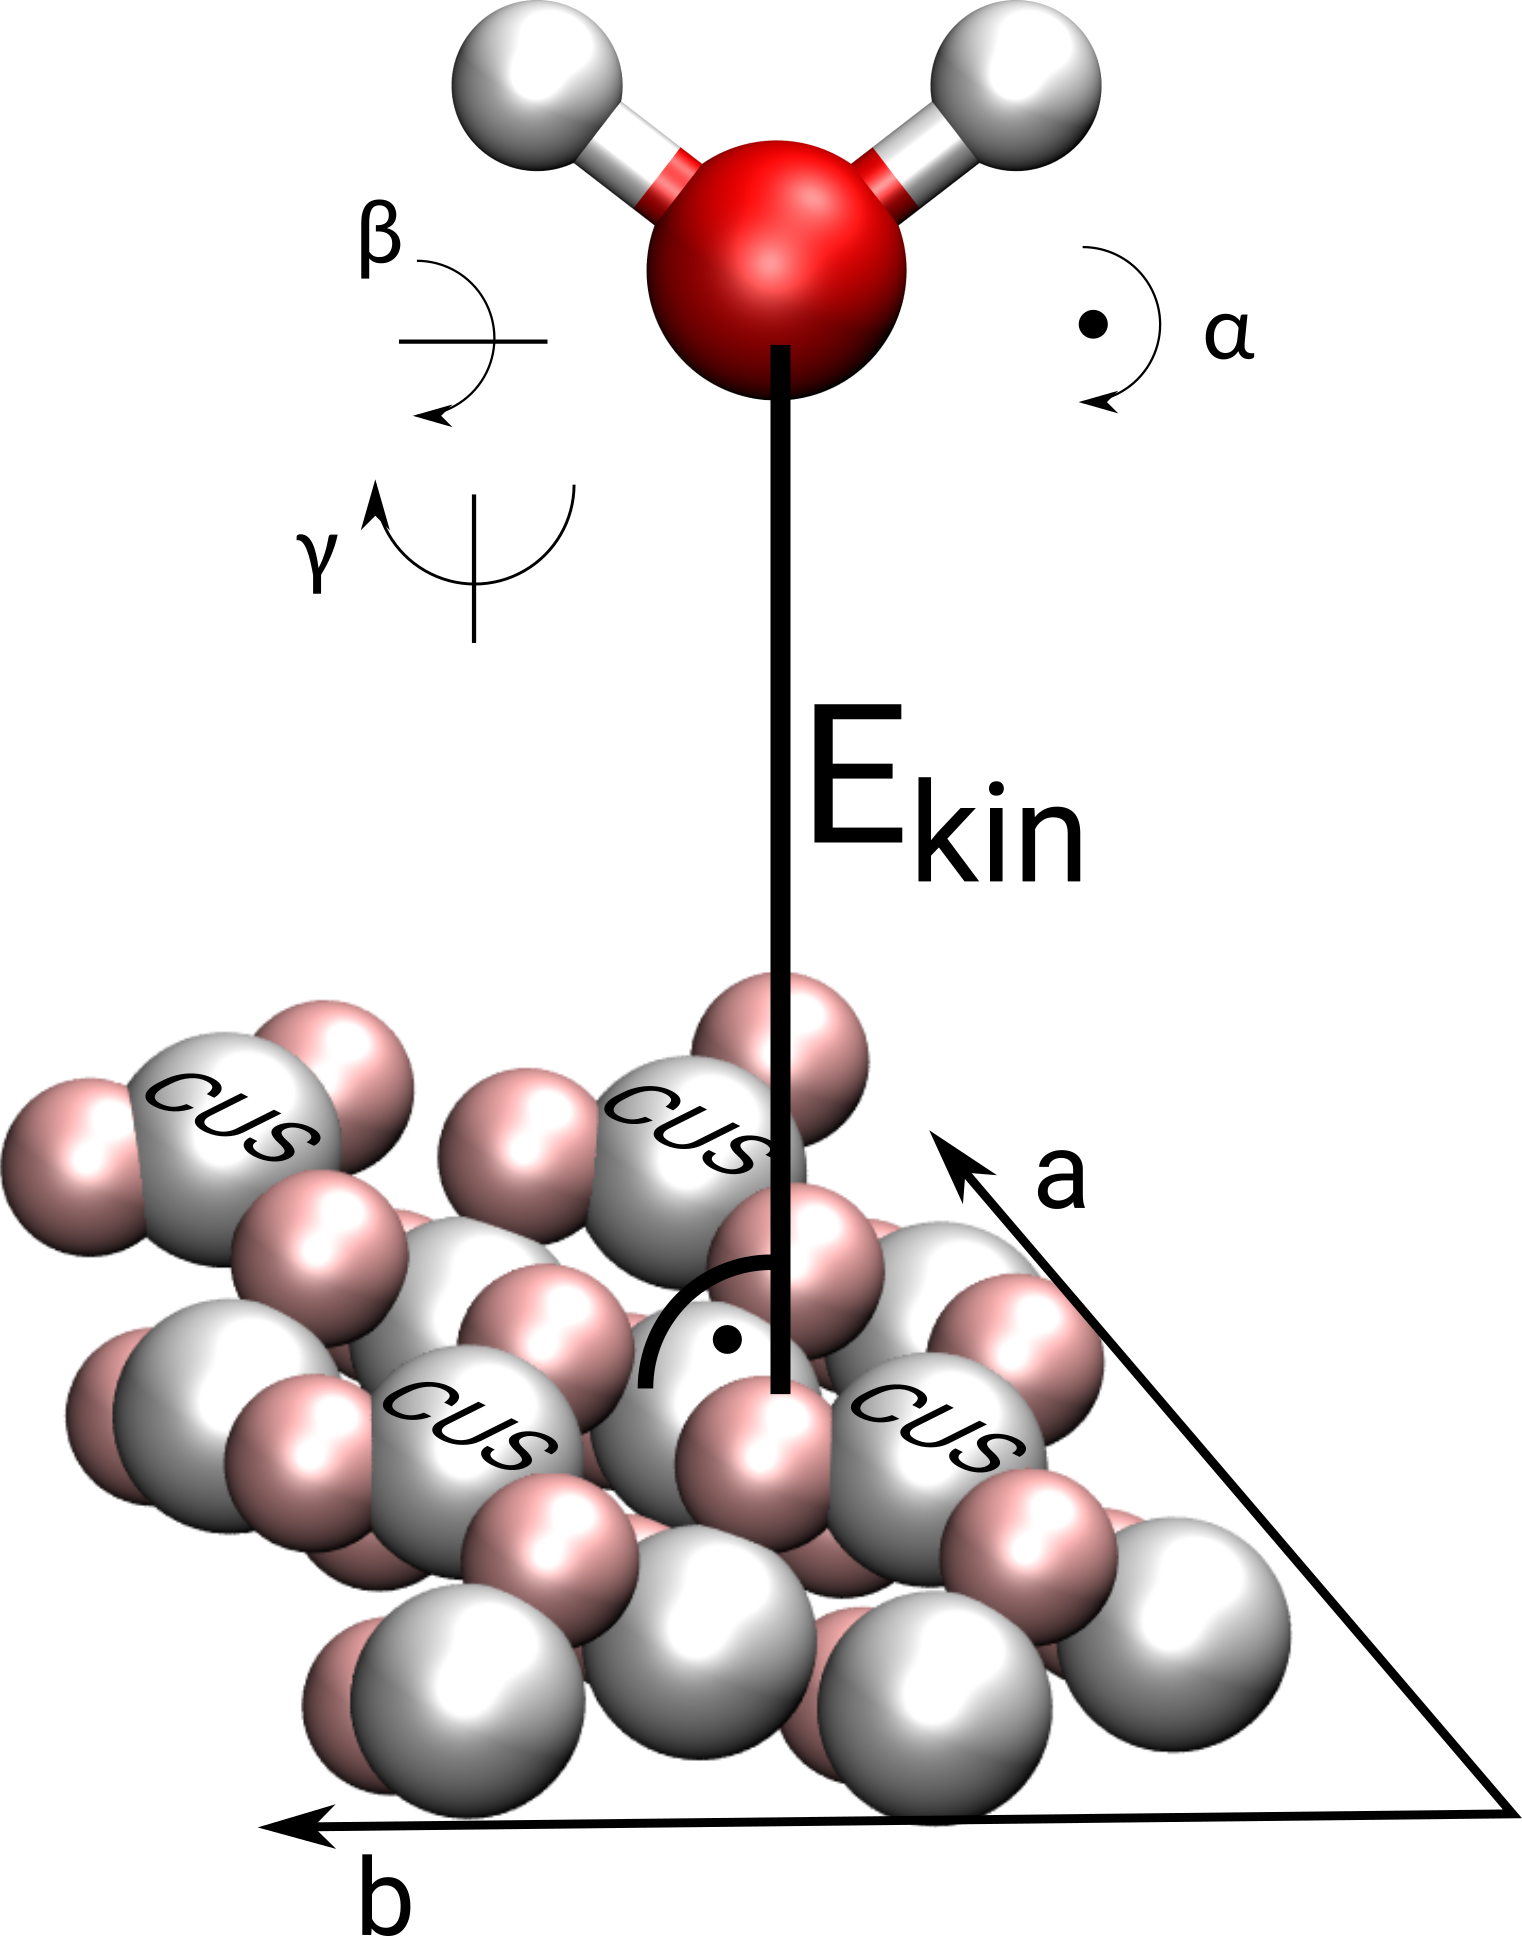
\includegraphics[width=0.25\textwidth]{figures/0001/perspective+h2o_new.png}
 \caption{Initial parameters of the trajectories, for MB scattering of D$_2$O at Al$_2$O$_3$(0001) considered in this work. Gray spheres Al, pale red O of alumina, red O and white H.
The water molecule approaches the surface perpendicular with its center of mass situated $4\,$\AA{} above the surface with a kinetic energy $E_\textrm{kin}$, at an impact site [$a_0,b_0$] given by fractions of the $\vec{a}$ and $\vec{b}$ vectors of the ($2\times 2$) cell.
The orientation is given by three Euler angles with respect to three perpendicular rotation axes, [$\alpha,\beta,\gamma$].}
        \label{abb:initial_parameters}
 \end{figure}
 
 \begin{figure}[h!]
 \centering
 \subfigure[{[0.33,0.33]}]{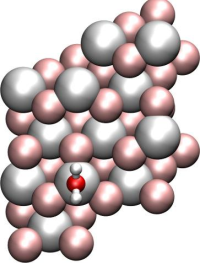
\includegraphics[angle=90, scale=0.45]{figures/0001/0_33-0_33test.png}}
          \quad
 \subfigure[{[0.5,0.5]}]{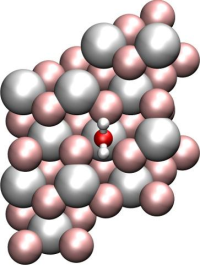
\includegraphics[angle=90,scale=0.45]{figures/0001/0_5-0_5test.png}}
         \quad
 \subfigure[{[0.35,0.5]}]{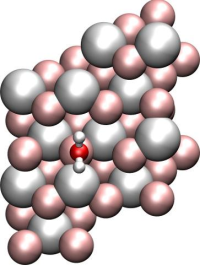
\includegraphics[angle=90,scale=0.45]{figures/0001/0_35-0_5test.png}}
        \\
 \subfigure[{[0.5,0.35]}]{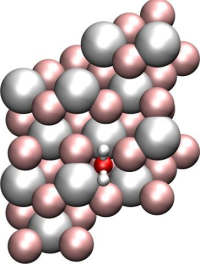
\includegraphics[angle=90,scale=0.45]{figures/0001/0_5-0_35test.png}}
        \quad
 \subfigure[{[0.35,0.45]}]{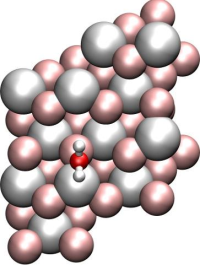
\includegraphics[angle=90,scale=0.45]{figures/0001/0_35-0_45test.png}}
        \quad
 \subfigure[{[0.4,0.5]}]{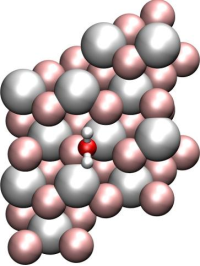
\includegraphics[angle=90,scale=0.45]{figures/0001/0_4-0_5test.png}}
 \caption{The six impact points $[a_0,b_0]$ which were used in the AIMD calculations (shown for the rotational orientation $[0,0,0]$, top view).
 %The different points reflect the most important sites of the surface.
%[0.33,0.33] is on top of an Al CUS, [0.5,0.5] on top of an Al in a subsurface layer.
% [0.35,0.5] is on top of a surface oxygen atom, whereas [0.5,0.35] is on top of a subsurface oxygen atom.
% [0.35,0.45] is in a gap between an Al CUS and a surface oxygen and [0.4,0.5] is in the gap between a surface O and a subsurface Al atom.
}
        \label{abb:impact_points}
 \end{figure}
 
 \begin{table}[!h]
 \centering
  \caption{Orientations of the water molecule characterized by three Euler angles [$\alpha,\beta,\gamma$], the latter given in \textdegree.
Shown are both top view and side view at impact point $[0.5,0.5]$.} %(look from the right-hand side of the top view).}
 \begin{tabular}{cp{4cm}p{4cm}}
 \toprule
orientation [$\alpha,~\beta,~\gamma$]& top view & side view \\\midrule
$[0, 0, 0]$  & 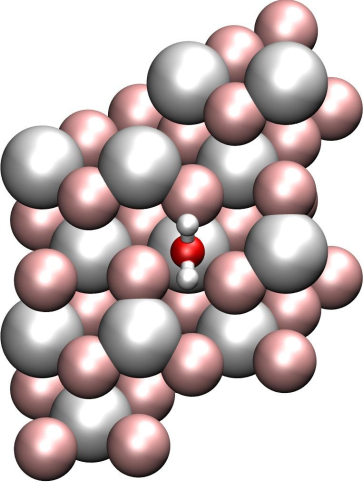
\includegraphics[width=2cm,angle=90]{figures/0001/Ausrichtungsbilder/0_0_0-toptest.png}
&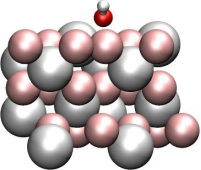
\includegraphics[width=2.5cm]{figures/0001/Ausrichtungsbilder/0_0_0-sidetest.png}\\
$[0, 0, 90]$   & 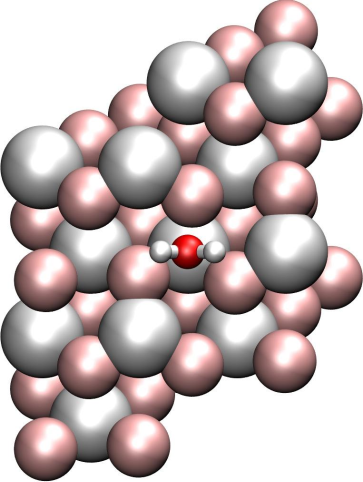
\includegraphics[width=2cm,angle=90]{figures/0001/Ausrichtungsbilder/0_0_90-toptest.png}
& 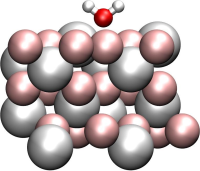
\includegraphics[width=2.5cm]{figures/0001/Ausrichtungsbilder/0_0_90-sidetest.png}\\
$[0, 90, 0]$   & 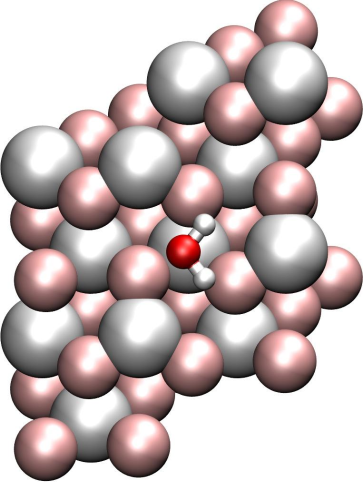
\includegraphics[width=2cm,angle=90]{figures/0001/Ausrichtungsbilder/0_90_0-toptest.png}
& 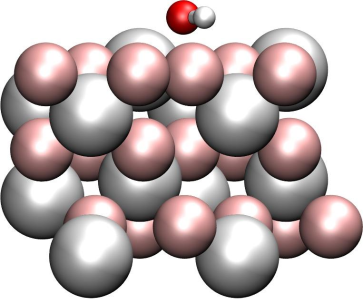
\includegraphics[width=2.5cm]{figures/0001/Ausrichtungsbilder/0_90_0-sidetest.png}\\
$[0, 90, 90]$ & 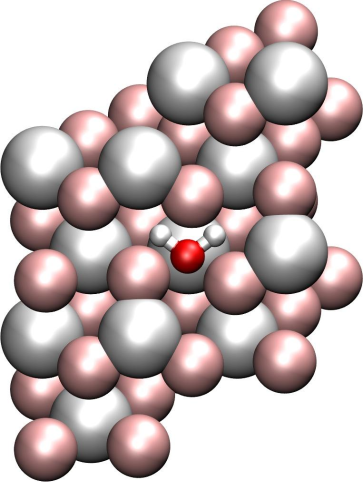
\includegraphics[width=2cm,angle=90]{figures/0001/Ausrichtungsbilder/0_90_90-toptest.png} 
& 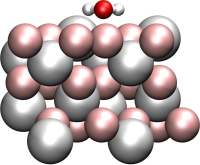
\includegraphics[width=2.5cm]{figures/0001/Ausrichtungsbilder/0_90_90-sidetest.png}\\
$[90, 0, 0]$ &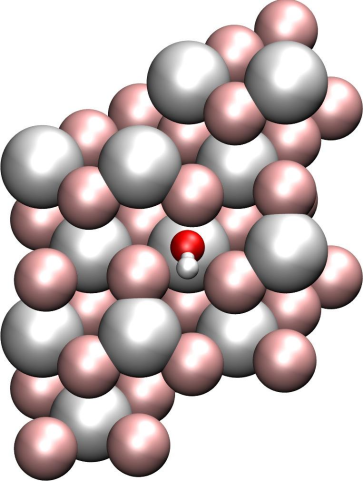
\includegraphics[width=2cm,angle=90]{figures/0001/Ausrichtungsbilder/90_0_0-toptest.png} 
& 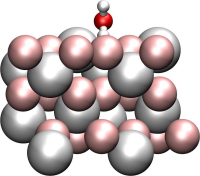
\includegraphics[width=2.5cm]{figures/0001/Ausrichtungsbilder/90_0_0-sidetest.png}\\
$[90, 0, 90]$ & 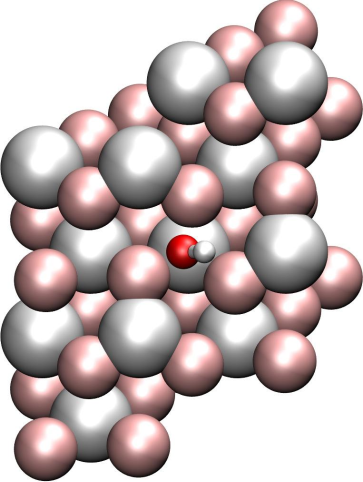
\includegraphics[width=2cm,angle=90]{figures/0001/Ausrichtungsbilder/90_0_90-toptest.png} 
& 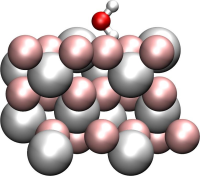
\includegraphics[width=2.5cm]{figures/0001/Ausrichtungsbilder/90_0_90-sidetest.png}\\
$[90, 90, 0]$ &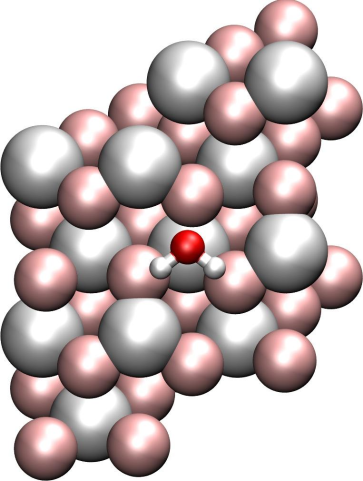
\includegraphics[width=2cm,angle=90]{figures/0001/Ausrichtungsbilder/90_90_0-toptest.png} 
& 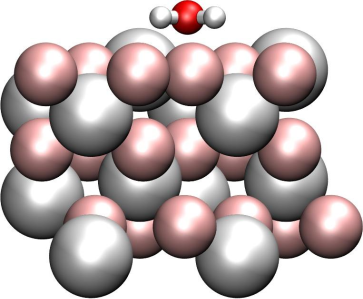
\includegraphics[width=2.5cm]{figures/0001/Ausrichtungsbilder/90_90_0-sidetest.png}\\
$[90, 90, 90]$ & 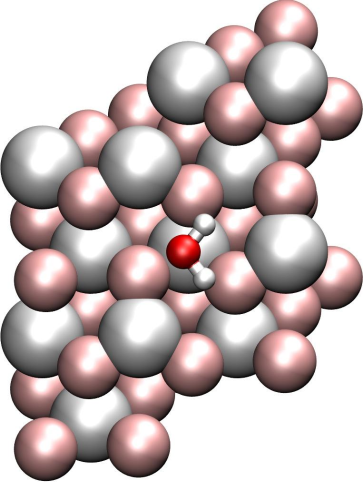
\includegraphics[width=2cm,angle=90]{figures/0001/Ausrichtungsbilder/90_90_90-toptest.png} 
& 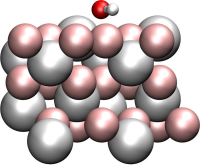
\includegraphics[width=2.5cm]{figures/0001/Ausrichtungsbilder/90_90_90-sidetest.png}\\\bottomrule
\end{tabular}
 \label{tab:orientations}
\end{table}
While many initial conditions were considered, it was not possible to compute a fully realistic beam, because this would require wide knowledge about energy and velocity distributions and a systematic high dimensional sampling.
This is not feasible with the computational power available for this work.
\clearpage
\subsection{Example Trajectories}
Before going to the details, example trajectories for each process leading to one of the four most stable adsorbed species, molecular adsorption, 1-2 dissociation, 1-4 dissociation and 1-4$^\prime$ dissociation are shown in Figure~\ref{abb:ex_traj}.
The applied parameters are reported in the respective caption.
These figures were all obtained from canonical calculations (NVT) at $300\,$K (the trajectory shown in (d) was additionally preexcited in the asymmetric stretch mode leading to 1-4$^\prime$ dissociation).
As one can see, molecular, 1-2 and 1-4 dissociated species can occur within sub-ps time scale at the surface; this process is henceforth called direct dissociation from the gas phase.
Note that in the 1-2 and 1-4 dissociated species, the dissociated deuteron undergoes large-amplitude motion, while the hydroxyl OD vibration is hardly excited after dissociation.
For the 1-4$^\prime$ dissociation shown in Figure \ref{abb:ex_traj}(d), such direct process does not happen.
Instead this species can be reached indirectly via a short-lived intermediate also within a sub-ps time scale. %, in this case the 1-2 species ca.$~40\,$fs later, so this is referred to as indirect dissociation with a molecular intermediate.
This is an example of a slow reaction (diffusion from 1-2 to 1-4$^\prime$ dissociated species with $\Delta G^\ddagger=0.67\,$eV\cite{WirthJPCC2012}) being enormously accelerated under MBS-like conditions.

This indirect process, however, is not unique for the 1-4$^\prime$ dissociated species, all the other species including the molecular one can be observed to happen indirectly by either being reflected first from the surface before adsorbing/dissociating or by adsorbing molecularly before dissociating.
However, the 1-4$^\prime$ species was the only one that could not be reached by direct dissociation.
  \begin{figure}[h!]
  \centering
   \subfigure[molecular adsorption]{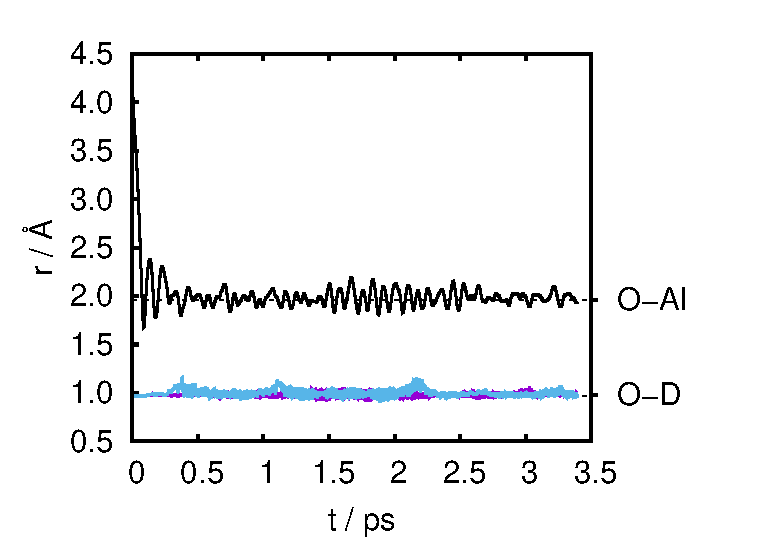
\includegraphics[width=0.4\textwidth]{figures/0001/graphs/mol.eps}}
   \quad
   \subfigure[1-2 dissociation]{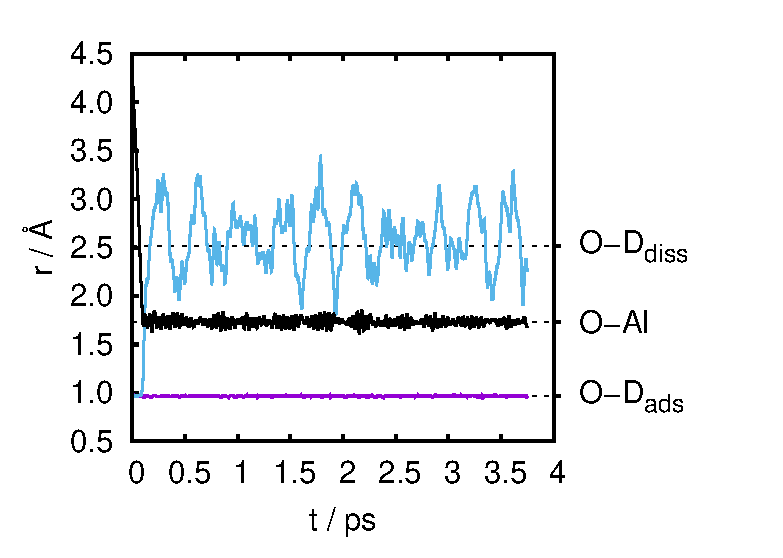
\includegraphics[width=0.4\textwidth]{figures/0001/graphs/1-2.eps}}
   \quad
   \subfigure[1-4 dissociation]{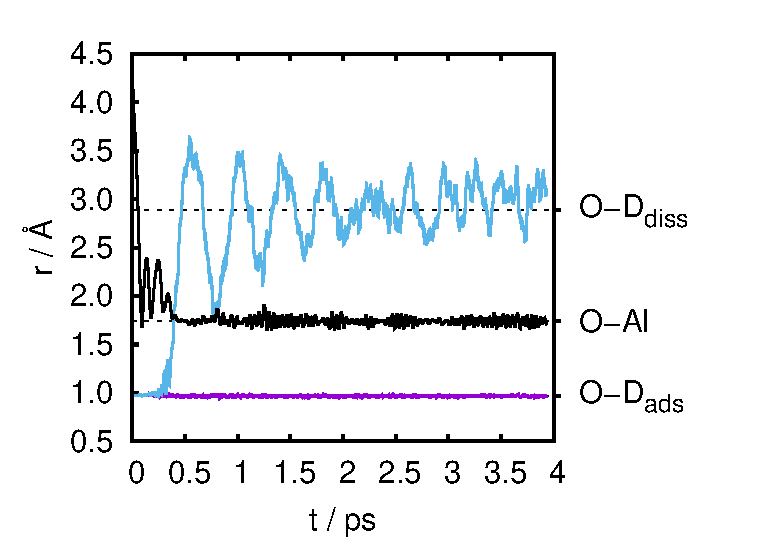
\includegraphics[width=0.4\textwidth]{figures/0001/graphs/1-4.eps}}
   \quad
   \subfigure[1-4$^\prime$ dissociation]{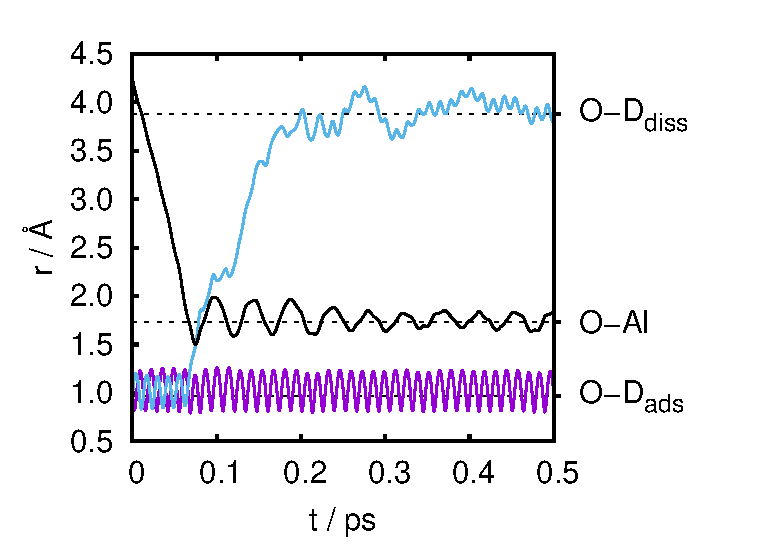
\includegraphics[width=0.4\textwidth]{figures/0001/graphs/1-4d.eps}}
% \begin{center}
% \hspace*{-1cm}
% \begin{tabular}{cc}
% \hspace*{-1cm}
% (a) molecular adsorption & (b) 1-2 dissociation \\
% {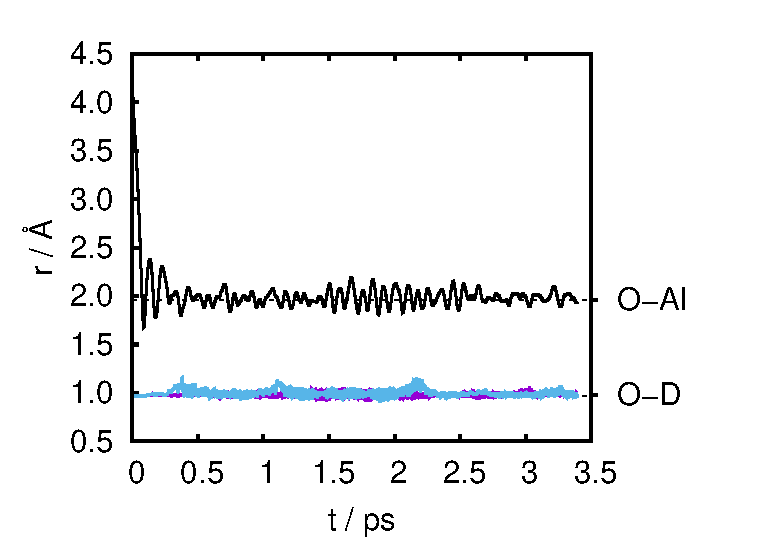
\includegraphics[width=0.4\textwidth]{figures/0001/graphs/mol.eps}}
%          &
% {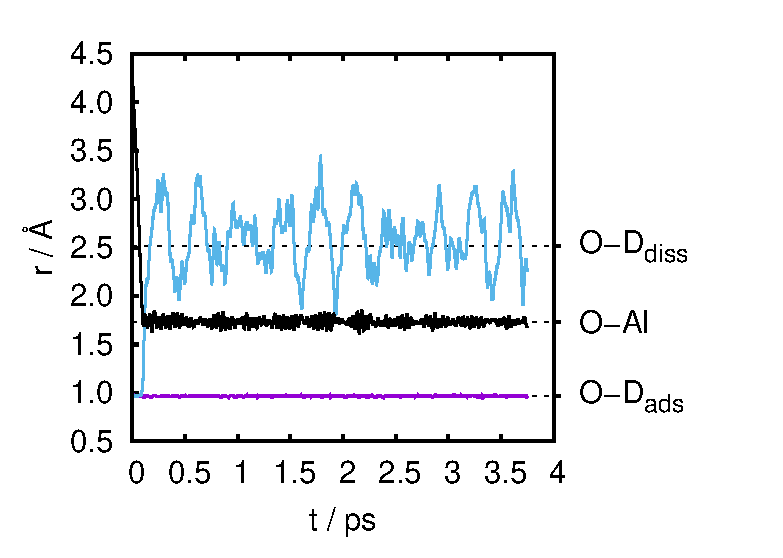
\includegraphics[width=0.4\textwidth]{figures/0001/graphs/1-2.eps}} \\
%  (c) 1-4 dissociation & (d) 1-4' dissociation \\
% {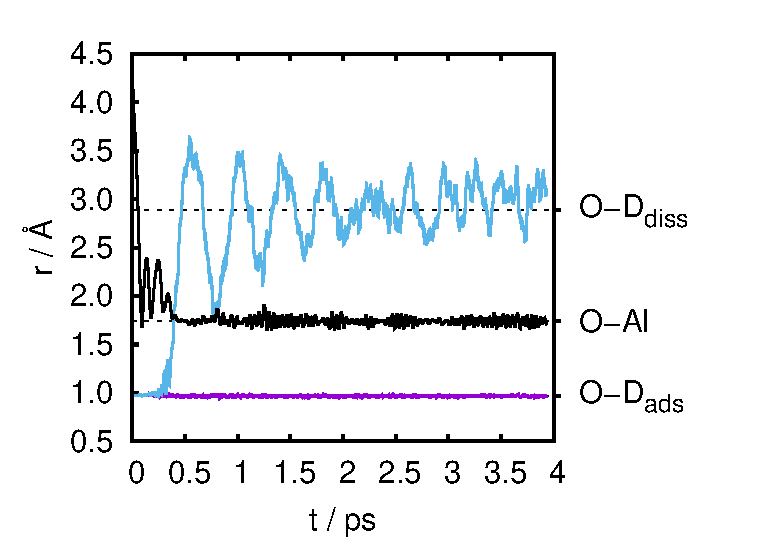
\includegraphics[width=0.4\textwidth]{figures/0001/graphs/1-4.eps}} &
% {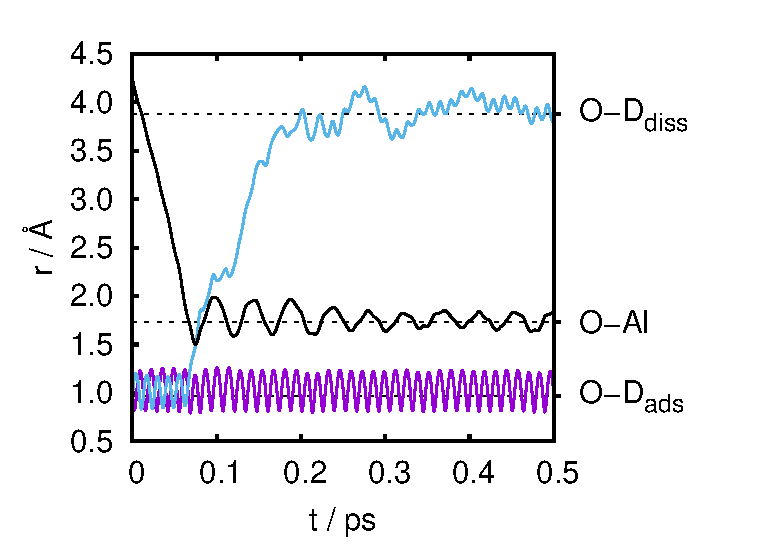
\includegraphics[width=0.4\textwidth]{figures/0001/graphs/1-4d.eps}}
% \end{tabular}
% \end{center}
\caption{The four adsorbed states of water, as shown in Figures \ref{abb:0001_ads}(a)-(d) are obtained in these exemplary trajectories.
All of them are from canonical (NVT) trajectories at  $T=300\,$K.
The initial parameters: (a) $E_\textrm{kin}=0.7\,$eV, $[a_0,b_0]=[0.33,0.33]$, $[\alpha,\beta,\gamma]=[0,0,90]$;
 (b) $E_\textrm{kin}=0.7\,$eV, $[a_0,b_0]=[0.35,0.45]$, $[\alpha,\beta,\gamma]=[0,0,0]$;
 (c) $E_\textrm{kin}=0.7\,$eV, $[a_0,b_0]=[0.33,0.33]$, $[\alpha,\beta,\gamma]=[0,90,0]$;
 (d) $E_\textrm{kin}=0.7\,$eV, $[a_0,b_0]=[0.35,0.5]$, $[\alpha,\beta,\gamma]=[0,0,0]$.
As specified in Subsection \ref{preex}, for the latter the water molecule was vibrationally preexcited along the asymmetric stretch normal coordinate.
The $r$ values (y axis) correspond to bond length distances between water-O and the CUS Al atom on which either D$_2$O or the water hydroxyl unit OD adsorb (O-Al), the distance between water-O and D in non-dissociated (fragments of) D$_2$O (O-D or O-D$_\textrm{ads}$), and the  distance between water-O and D in dissociated (fragments) of D$_2$O (O-D$_\textrm{diss}$), respectively.
Also the interatomic distances of the minimum geometries are given as horizontal dashed lines.
Panel (d) shows that the 1-4$^\prime$ state is not obtained directly but reached \textit{via} a short-lived 1-2 dissociation intermediate.}
\label{abb:ex_traj}
\end{figure}


\subsection{Microcanonical AIMD at a Clean Surface at $T=0$}\label{sec:mic_clean}
The effects of a single D$_2$O shot to the cool surface with an NVE ensemble (microcanonical AIMD, the $0\,$K optimized geometry of the surface has no initial momenta) were studied systematically by probing over six parameters: Five different kinetic energies (from $0.5$ to $0.9\,$eV in $0.1\,$eV steps), six lateral impact points at the surface ([0.33,0.33], [0.5,0.5], [0.35,0.5], [0.5,0.35], [0.35,0.45], [0.4,0.5], as introduced in Figure \ref{abb:impact_points}), and eight different orientations of the water molecule with respect to the surface ([0,0,0], [0,0,90], [0,90,0], [0,90,90], [90,0,0], [90,0,90], [90,90,0], [90,90,90], see also Table \ref{tab:orientations}).
These $5\times 6\times 8=240$ AIMD trajectories for the clean surface at $T=0\,$K were simulated for ca.$~1.2\,$ps each.


In the trajectories  either molecular adsorption, 1-2 dissociation or reflection could be observed.
Dissociation was assumed if the OD distance was greater than $1.3\,$\AA{}, but it was ensured that the results did not differ for a greater cutoff distance by looking at each individual trajectory.
Interestingly, only 1-2 dissociation and no 1-4 dissociation could be observed for these conditions (NVE, clean surface), although the molecular and the 1-4 dissociated species are almost equal in energy, and also the barrier heights $\Delta E^\ddagger$ for the dissociation to 1-2 ($0.13\,$eV) and 1-4 ($0.19\,$eV) do not differ largely\cite{WirthJPCC2012}. %(\textit{cf.} Table \ref{tab:0001_rates}).
As shown later, other conditions are necessary for reaching 1-4 dissociation.
\\
  \begin{figure}[!h]
\centering
 \subfigure[Energy]{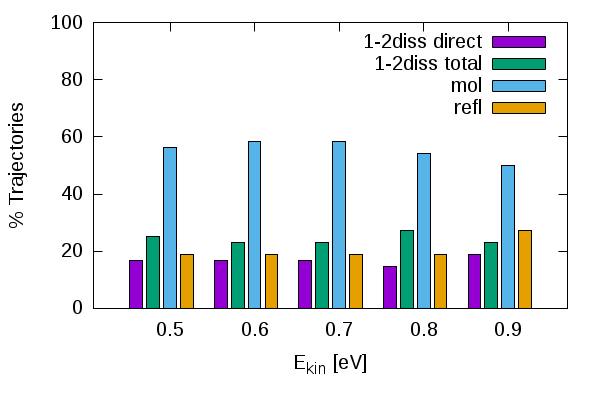
\includegraphics[width=0.5\textwidth]{figures/0001/graphs/E.png}} 
 \quad
 \subfigure[Impact Point]{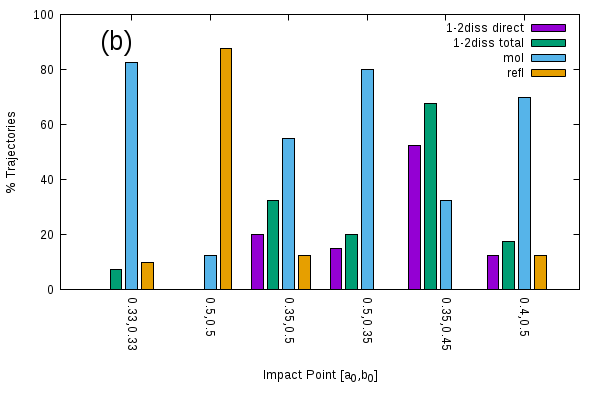
\includegraphics[width=0.5\textwidth]{figures/0001/graphs/impactpoint.png}} 
 \quad
 \subfigure[Orientation]{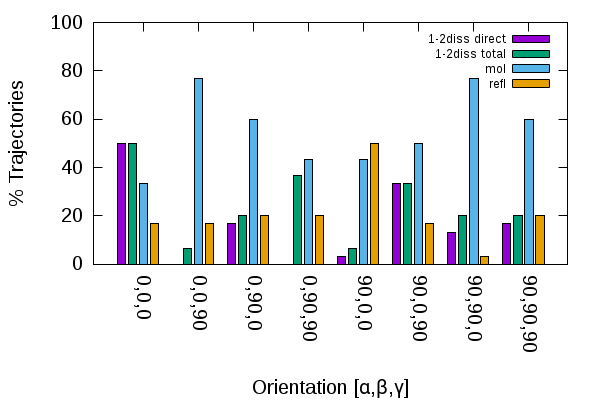
\includegraphics[width=0.5\textwidth]{figures/0001/graphs/orientation.png}}
\caption{Bar charts showing the statistics of NVE AIMD trajectories at $0\,$K for a single D$_2$O molecule approaching the clean alumina(0001) surface.
(a) summarizes the findings for all kinetic energies $E_\textrm{kin}$ averaged over $6\times 8=48$ combinations of impact point and orientation.
In (b), for all impact points $[a_0,b_0]$ is averaged over $5 \times 8=40$ combinations of kinetic energy and rotational orientation and (c) gives an overview over all rotational orientations $[\alpha,\beta,\gamma]$, averaged over $5 \times 6=30$ combinations of kinetic energy and impact points.
The columns give percentages of the different outcomes - here labeled as direct and total 1-2 dissociation (``1-2 diss direct'' in purple and  ``1-2 diss total'' in green), ``mol'' molecular adsorption (blue) and ``refl'' reflection in yellow.
If one type of outcome did not occur, no column is shown.}
\label{abb:barchart_mic}
\end{figure}

As an example and also for later reference, we list in Table \ref{tab:NVE-clean},  the outcomes of all 48 trajectories for a particular kinetic energy, $E_\textrm{kin}=0.7\,$eV, which illustrates the points just made.
In this case, molecular adsorption dominates, followed by 1-2 dissociation and reflection.
\\
\begin{table}[!h]
  \centering
  \caption{Outcome of microcanonical (NVE, $T=0$) trajectories with $E_{\textrm{kin}}=0.7\,$eV, after the end of propagation, for different combinations of initial impact points and rotational orientations.
  R=reflection, M=molecular adsorption, D(1-2)=1-2 dissociation.}
  \begin{tabular}{l|cccccc}
    \toprule
    orientation& \multicolumn{6}{c}{impact position $[a_0,b_0]$} \\
    $[\alpha,\beta,\gamma]$ & [0.33,0.33] & [0.5,0.5] & [0.35,0.5] & [0.5,0.35] & [0.35,0.45] & [0.4,0.5] \\
    \midrule
  $[0,0,0]$    &M &R &D(1-2) &M &D(1-2) & D(1-2)\\
  $[0,0,90]$  &M &R &M & M  & M & M\\
  $[0,90,0]$  &M &R &M & M  &D(1-2) & M \\
  $[0,90,90]$ &D(1-2) &R & M &M &D(1-2) & M\\
  $[90,0,0]$   &M &R &R & M  & M &R \\
  $[90,0,90]$ &M &R &M &D(1-2) &D(1-2) & M \\
  $[90,90,0]$  &M &M &D(1-2) &M &D(1-2) & M \\
  $[90,90,90]$ &M &R &M &M  &D(1-2) &M \\
    \bottomrule
  \end{tabular}
  \label{tab:NVE-clean}
\end{table}

Figure~\ref{abb:barchart_mic} is a statistical analysis of the data, where the probabilities for reflection, molecular adsorption and 1-2 dissociation are shown as a function of the kinetic energy (a), impact point (b) and the orientation (c).
It was distinguished between direct and indirect dissociation.
Admittedly, this analysis is restricted by the number of trajectories (240).
From these figures and the data one can derive the following conclusions:


As anticipated, all three processes could be observed, reflection ($20.4\%$, 49 of the 240 trajectories), molecular adsorption ($55.4\%$, 133 trajectories) and 1-2 dissociation ($24.2\%$, 58 trajectories).
Probabilities for all outcomes can be found in Appendix \ref{reactionprobabilities}.


Looking at the influence of the kinetic energy in Figure \ref{abb:barchart_mic}(a), the results do not depend largely on the initial kinetic energy of the molecule, at least for the probed energy range.
In all cases molecular adsorption dominates, followed by 1-2 dissociation and reflection, both of which are in the same range around $20$-$25\%$.
This reflection probability P$_\textrm{diss}$ is only increased for $0.9\,$eV, at the expense of the molecular species.\\
We chose the set of parameters ([$a_0,b_0]=[0.35,0.45]$; $[\alpha,\beta,\gamma]=[0,0,0]$), for which $P_\textrm{diss}=1$ for all energies $\geq 0.5\,$eV.
To evaluate whether this will hold true for the low energy regime, one additional trajectory with the kinetic energy of $0.1\,$eV was calculated.
In the case of E$_\textrm{kin}=0.1\,$eV, the trajectory only shows molecular adsorption.
This result was rather surprising, since the kinetic energy plus the adsorption energy minus the barrier height is with $(0.1+1.31-0.13)\,$eV=$0.28\,$eV in the same order as the reaction barrier ($\Delta G^\ddagger=0.29\,$eV\cite{WirthJPCC2012}). %, compare Table \ref{tab:0001_rates}).
%It seems that the excess energy is not available for the OD bond breaking and instead relaxes in other degrees of freedom of the system.
This allows to draw the conclusion that a minimum kinetic energy is necessary for the dissociation process.
In the experimental studies of R. K. Campen\cite{Heiden11-20_2018}, a kinetic energy of the beam between $0.6$ and $0.75\,$eV is used.
This minimum energy constraint can be one possible explanation of the difference between MBS and pinhole dosing.
In the latter case, the only energy of a water molecule comes from the thermal energy.
For a D$_2$O molecule in the gas phase at $300\,$K this can be estimated to be around $\frac{3}{2}k_BT\approx40\,$meV.


In contrast to the kinetic energy, the lateral impact point at the surface has a great influence on adsorption and dissociation probabilities as can be seen in Figure \ref{abb:barchart_mic}(b).
For the impact point [0.5,0.5], a non-surface Al position, $88\%$ of the trajectories get reflected and molecular adsorption and 1-2 dissociation are oppressed, whereas for [$0.33,0.33$], directly on top of an Al CUS position, $83\%$ adsorb molecularly which dominates clearly over 1-2 dissociation.
In contrast to both sites, [$0.35,0.45$] which is located at a gap between the CUS position and a neighboring oxygen atom leads to a high dissociation probability of P$_\textrm{diss}\approx 68\%$ with a minor percentage of indirect dissociation.
This high dissociation probability can be explained by the fact that the molecule hits the surface already in a ``product-like'' geometry, so that the OD bond breakage is facilitated.


The initial rotational orientation also has an effect (\textit{cf.} Figure \ref{abb:barchart_mic}(c)), although not as drastic as the impact point dependence.
This might be explained when looking at the trajectories in detail, where one can see that the water molecule rotates due to the attractive and repulsive interaction with the surface atoms.
This leads to a reorientation of the water molecule right before adsorbing, so that the initial orientation is not remembered reliably by the system.
The orientation of the molecule shortly before reaching the surface is more important.
As before, if the molecule's orientation is already in a product-like state, the dissociation probability is elevated.


The data shows that direct dissociation dominates mostly over indirect dissociation, although it is dependent on the initial conditions, \textit{e.
g.} for the initial orientation [0,90,90] only indirect dissociation is observed.

 \clearpage
\subsection{Thermalized Surface}\label{therm_surf}
The effects of a thermal surface were studied for single D$_2$O molecules approaching a clean $\alpha$-Al$_2$O$_3$(0001) surface, using an initial kinetic energy of $0.7\,$eV with momentum perpendicular to the surface.
First, we selected five initial parameter sets, which all led to (1-2) dissociation in the microcanonical (NVE, $T=0$) case: $[a_0,b_0],[\alpha,\beta,\gamma]=$ $[0.35,0.45],[0,0,0]$; $[0.35,0.45],[0,90,90]$; $[0.35,0,45],[90,90,90]$; $[0.4,0.5],[0,0,0]$;  $[0.5,0.35],[90,0,90]$.
For all of these sets, 100 NVT trajectories were run at a temperature of $300\,$K, following the protocol: (1) The naked surface was preequilibrated for $1\,$ps; (2) then the water was fired using an analogous setting as in Section \ref{sec:mic_clean} on the thermal surface now, and the AIMD trajectories were run for another 1-ps period. For testing longer propagation periods, see below.
In practice in step (2), the thermostat acted also on water, however, since the molecule quickly hits the surface (400 steps, $\sim$0.08$\,$ps), this slight inconsistency hardly affects the dynamics.
\\

As a result of this procedure, we found that \textit{all} 500 trajectories (100 trajectories $\times$ 5 parameter sets) led to 1-2 dissociation.
No reflection, molecular adsorption and other modes of dissociation (1-4 or 1-4$^\prime$) were observed, at least on the time scale considered.
The inefficiency of thermal surface motion was slightly surprising (and disappointing) to us, since the energy of a thermalized surface, $\sim N_s \times 3 k_B T = 2.8\,$eV (where $N_s=36$ is the number of movable surface atoms), is comparable to the kinetic energy of the molecule when crashing into the surface ($\sim$2$\,$eV). On the other hand, when only a single surface atom (\textit{e.g.}, an impact site) is considered, the surface atom's energy is much smaller than that of the impinging molecule which may rationalize the observation.
\\

Next, all $6\times 8=48$ combinations of impact sites $[a_0,b_0]$ and rotational orientations  $[\alpha,\beta,\gamma]$ as in Section \ref{sec:mic_clean} were (re-)considered, for a single initial translational energy of $E_\textrm{kin}=0.7\,$eV.
Now, only two NVT AIMD calculations were run per initial condition, after the surface had been equilibrated at $300\,$K for $1\,$ps before.
The restriction to two trajectories gives only a quite limited statistical significance but was dictated by restricted computational resources.
We did allow for longer propagation times after the equilibration phase, though, propagating  each trajectory for $4\,$ps now.
For six of the 48 initial conditions, our NVT AIMD trajectories terminated due to numerical problems.
For the remaining $42\times2=84$ AIMD trajectories, a ``statistics'' for various events, reflection, molecular and dissociative adsorption, was obtained as shown in Table \ref{tab:nvt-nve_comp}, third line.
These values are to be compared to the corresponding 42 microcanonical, $T=0$ trajectories for $E_\textrm{kin}=0.7\,$eV, given in the second row of Table \ref{tab:nvt-nve_comp}.
For reference, the corresponding values for $E_\textrm{kin}=0.7\,$eV averaged over all 48 initial conditions (see also Figure \ref{abb:barchart_mic}(a) and Table \ref{tab:NVE-clean}), are given in the first row of the table.
Probabilities for other impact energies are supplied in Appendix \ref{reactionprobabilities}.
\\
\begin{table}[!h]
 \centering
 \caption{Statistical results for NVE (upper two rows) and NVT trajectories at $300\,$K (lower row).
The models differ only by the thermalized surface, for all trajectories a single D$_2$O was sent on a clean surface with a kinetic energy of E$_\textrm{kin}=0.7\,$eV.
The initial parameters were the 48 and selected 42 from Section \ref{sec:mic_clean}, respectively, as explained in the text.}
\vspace*{.2cm}
  \begin{tabular}{lc|cccc}
 \toprule
  ensemble & no.
of trajectories & $P_\textrm{refl}$ & $P_\textrm{mol}$ & $P_\textrm{diss}$ (1-2) & $P_\textrm{diss}$(1-4) 
 \\\midrule
 NVE$^1$         & 48 & 0.19 & 0.58 & 0.23 & 0.00 \\
 NVE$^{1,3}$     & 42 & 0.19 & 0.55 & 0.26 & 0.00 \\
 NVT$^2$ &$42\times 2$& 0.12 & 0.54 & 0.24 & 0.11 \\\bottomrule
  \end{tabular}
\begin{tablenotes}
 \footnotesize
\item[] $^1$ Propagation time $1.22\,$ps.
$^2$ Propagation time $4\,$ps.
$^3$ A subset of the NVE/48 data set,  corresponding to the same initial impact parameters as used for the NVT ensembles.
\end{tablenotes}
\label{tab:nvt-nve_comp}
\end{table}



Thus, compared to the corresponding microcanonical trajectories (for 42 initial impact parameters), for the thermal surface we see the following differences: (i) The reflection probability is diminished (from 0.19 to 0.12); (ii) molecular adsorption is not much affected: a bit more than half of the trajectories adsorb molecularly in both cases; (iii) the \textit{total} dissociation probability is increased (from 0.26 to 0.35); (iv) 1-4 dissociation appears in the thermal case to some extent.
Among the 1-4 dissociations (nine trajectories out of 84), four reacted directly and five indirectly, \textit{via} a molecular adsorbate.
Note that all nine 1-4 dissociated trajectories led to molecular adsorption under microcanonical ($T=0$) conditions.
Despite  the statistical limitiations and short trajectories we note that surface temperature seems to have some effect, in particular on the probability and type of dissociation.
Further inspection of the canonical / NVT trajectories shows that among the cases leading to molecular adsorption after $4\,$ps, also trajectories were found in which D$_2$O ended up at different Al CUS sites than expected from the position of first impact, due to molecular diffusion on the surface and / or trajectories undergoing multiple bounces.


% After gaining an impression of the system with the microcanonical MD at the clean surface, as a next step the thermalized surface at $300\,$K is studied.
% One has to keep in mind, that in contrast to NVE, NVT (canonical) is nondeterministic.
% This means a given set of parameters has to be simulated multiple times in order to draw statistically relevant conclusions.
% The naked surface was preequilibrated at $300\,$K for $1\,$ps and the obtained geometry with respective velocities was used as an input to the following calculations.
% Here, only a kinetic energy of $0.7\,$eV was considered, since this energy is the closest to previous experiments by Campen and more importantly the energy dependence was shown to be insignificant in NVE trajectories, assuming this is still valid at $300\,$K.
% The water molecule was then shot onto the equilibrated surface.
% The heat bath acted on the water molecule from the start.
% This is not huge a problem, since the molecule hits the surface quickly and thus this detail hardly affects the dynamics.
% 
% 
% First, for a selection of five parameter sets 100 NVT trajectories were calculated each at a temperature of $300\,$K.
% These parameter sets are\\ $[a_0,b_0][\alpha,\beta,\gamma]$= $[0.35,0.45]$,$[0,0,0]$; $[0.35,0.45]$,$[0,90,90]$; $[0.35,0,45]$,$[90,90,90]$; $[0.4,0.5]$,$[0,0,0]$;  $[0.5,0.35]$,$[90,0,90]$.\\
% In the previous microcanonical simulations these parameters led to 1-2 dissociation and were chosen based on the assumption that the thermal effects might trigger the impinging water molecules to dissociate or to diffuse to the 1-4 species.
% The trajectories were computed analogously as in Section \ref{sec:mic_clean} except for now the thermalized surface for a duration of $1\,$ps each.
% All of these 500 trajectories led to dissociation to the 1-2 species; no reflection, molecular adsorption or further dissociation could be observed.
% As it seems, the thermal contribution is low, which was unexpected.
% % The energy of the thermalized surface can be estimated by $N_s\times 3k_BT=2.8\,$eV (with $N_s=36$ being the number of atoms in the surface slab which were allowed to relax/move).
% % This energy is in the same range as the kinetic energy of the incoming water molecule ($\approx2\,$eV).
% % Indeed, this surface energy is not valid for the small surface range where the impact takes place, so that the thermal energy of the atom(s) of the impingement is considerably smaller.
% 
% 
% As a next step, all $6\times 8=48$ combinations of the six impact points and eight orientations presented in Section \ref{sec:mic_clean} were evaluated using the thermalized surface, but only for a kinetic energy of $0.7\,$eV.
% For each of the sets, two trajectories of $4\,$ps duration were calculated.
% This restriction is due to high computational costs and results in a limited statistical significance.
% The long duration accounts for processes occuring later after the impact that could have been missed by shorter trajectories.
% In Table \ref{tab:nvt-nve_comp}, the probabilities for each process are shown in comparison with the previous microcanonical AIMD trajectories.
% Because six of the trajectories aborted due to numerical reasons, here only 42 trajectories can be evaluated and the comparison is, of course, made only with the corresponding microcanonical trajectories.
% \begin{table}[!h]
%  \centering
%  \caption{Statistical results for NVE (both upper lines) and NVT trajectory at $300\,$K (lower line).
% The models differ only by the thermalized surface, for all trajectories a single D$_2$O was sent on a clean surface with a kinetic energy of E$_\textrm{kin}=0.7\,$eV.
% The initial parameters were the 48 and selected 42 from Section \ref{sec:mic_clean}, respectively, as explained in the text.}
% \vspace*{.2cm}
%   \begin{tabular}{lc|cccc}
%  \toprule
%   ensemble & no.
% of trajectories & $P_\textrm{refl}$ & $P_\textrm{mol}$ & $P_\textrm{diss}$ (1-2) & $P_\textrm{diss}$(1-4) 
%  \\\midrule
%  NVE$^1$         & 48 & 0.19 & 0.58 & 0.23 & 0.00 \\
%  NVE$^{1,3}$     & 42 & 0.19 & 0.55 & 0.26 & 0.00 \\
%  NVT$^2$ &$42\times 2$& 0.12 & 0.54 & 0.24 & 0.11 \\\bottomrule
%   \end{tabular}
% \begin{tablenotes}
%  \footnotesize
% \item[] $^1$ Propagation time $1.22$ ps.
% $^2$ Propagation time 4 ps.
% $^3$ A subset of the NVE/48 data set,  corresponding to the same initial impact parameters as used for the NVT ensembles.
% \end{tablenotes}
% \label{tab:nvt-nve_comp}
% \end{table}
% In the first line of the table, the results for the complete probed space for the NVE (T=0) is shown, the second line gives the results for the corresponding 42 microcanonical trajectories and in the third line, the canonical results for 42 NVT trajectories ($T=300\,$K) are given.
% For all, the kinetic energy is $E_\textrm{kin}=0.7\,$eV.
% In contrast to the microcanonical MD, the canonical yields 1-4 dissociation at a percentage of around $11\%$ and gives slight decreases in the reflection, whereas molecular adsorption and 1-2 dissociation almost remain constant.
% Of the 1-4 dissociated trajectories, $44\%$ dissociated directly and $56\%$ indirectly after initial molecular adsorption.
% Interestingly, all initial conditions in the trajectories that show 1-4 dissociation in the NVT led only to molecular adsorption in the NVE AIMD.
% The idea supposed earlier assumed 1-4 dissociation from trajectories that gave 1-2 dissociation in NVE, but apparently the molecular species plays a more important role.
% 
% 
% Note that the surface temperature indeed has an effect on the probabilities for the different processes and also 1-4 dissociation could be observed.
% As before, the first impact can lead to reflection and in a ``bouncing'' process, the molecule can also adsorb after another impact, in few cases also on another CUS atom as the initial impact was on.
 
\subsection{Refined Surface Model}
During a MBS experiment, after some time the surface will be precovered with water (fragments), which in turn will affect the reactivity of further molecules approaching the surface.
In order to study the effects of precoverage, we considered a single water (D$_2$O) molecule on a ($2\times 2$) $\alpha$-Al$_2$O$_3$(0001), adsorbed as shown in Figure \ref{abb:0001_ads}, either molecularly (a), as 1-2 dissociated species (b), or as 1-4 dissociated species (c).
Note that in all cases, the water or hydroxyl group is adsorbed in the lower right ($1\times 1$) sub-cell, on the CUS Al site at lateral position $[0.33,0.33]$ (\textit{cf.} Figure \ref{abb:impact_points}(a)).
\\

We now fire a second D$_2$O molecule with an initial kinetic energy of $E_\textrm{kin}=0.7\,$eV onto the surface as described in the previous section(s), choosing various rotational orientations and impact sites.
The total propagation time is $1\,$ps.
The selected, lateral impact points $[a_0,b_0]$ were chosen to be  (i) either in the lower-right ($1\times 1$) sub-cell close to the Al CUS where the preadsorbed water (fragment) is situated, or (ii) in a neighbor (the lower left) ($1\times 1$) sub-cell around the corresponding CUS there.
Individual trajectories are analyzed with respect to two criteria: (i) Their influence on the preadsorbed molecule (or molecular fragment), and (ii) the (reactive) behavior of the second, incoming molecule.
We do this first for $T=0$, using NVE AIMD calculations as in Section \ref{sec:mic_clean}. 
\\


Let us consider what happens when D$_2$O hits the ($1\times 1$) subcell with already preadsorbed water (fragments).
In Table \ref{tab:preads_mic}, we list in analogy to Table \ref{tab:NVE-clean}, the outcomes  of a subset of NVE trajectories for two selected impact sites $[a_0,b_0]=[0,33,0.33]$ (\textit{i.e.}, direct hit of preadsorbed water or water fragment), and $[a_0,b_0]=[0,35,0.45]$ (\textit{i.e.}, slightly nearby the Al CUS site, see Figure \ref{abb:impact_points}(e)).
The table gives information for all preadsorption cases: molecular, 1-2 dissociated and 1-4 dissociated.
In contrast to Table \ref{tab:NVE-clean}, we show \textit{two} symbols for each entry, \textit{e.g.}, ``M, D(1-2)'' to illustrate the fates both of the incoming molecule (the first symbol, ``M'' in this case) and the preadsorbed species (the second symbol, ``D(1-2)'' in this example).
Further, a star ($*$) has been added to the second symbol, if the character of the preadsorbed species changed during the scattering process.
\\
\begin{table}[!h]
  \centering
  \caption{Selected results of preadsorbed surface trajectories for the microcanonical ensemble (NVE, $T=0\,$K, E$_\textrm{kin}=0.7\,$eV).
The three investigated cases are: molecular, 1-2 and 1-4 dissociated preadsorption.
R=reflection, M= molecular adsorption (chemisorption), P=molecular physisorption, D(1-2)=1-2 dissociation, D(1-4)=1-4 dissociation.
The two letters for each cell give the outcomes for the \textit{incoming} molecule (first entry) and the \textit{preadsorbed} water (second entry).
For the case, that the preadsorbed species changed its character, a $^*$ is attached.
``term.'' refers to terminated trajectories.
Missing entries mean that no calculation was performed.}
\hspace*{-1cm}
 \begin{tabular}{l|cc|cc|cc}
 \toprule
               & \multicolumn{6}{c}{type of preadsorption } \\\hline
               & \multicolumn{2}{c|}{molecular} & \multicolumn{2}{c|}{1-2 dissociated} & \multicolumn{2}{c}{1-4 dissociated} \\\hline
    orientation& \multicolumn{2}{c|}{impact position $[a_0,b_0]$} & \multicolumn{2}{c|}{impact position $[a_0,b_0]$} & \multicolumn{2}{c}{impact position $[a_0,b_0]$} \\
    $[\alpha,\beta,\gamma]$ & [0.33,0.33] & [0.35,0.45] & [0.33,0.33] & [0.35,0.45] & [0.33,0.33] & [0.35,0.45] \\
    \midrule
   $[0,0,0]$    &          & P, D(1-2)$^*$  &  & M, D(1-2) &  & R, D(1-4) \\
   $[0,0,90]$   &          & M, D(1-2)$^*$  &  & M, D(1-2) &  & P, D(1-4) \\
   $[0,90,0]$   & M, D(1-2)$^*$ & P, D(1-4)$^*$  & R, D(1-2) & M, D(1-2) & R, D(1-4) & P, D(1-4) \\
   $[0,90,90]$  &          & P, D(1-4')$^*$ &  & M, D(1-2) &          & term. \\
   $[90,0,0]$   &          & P, D(1-2)$^*$  &  & M, D(1-2) &  & M, D(1-4) \\
   $[90,0,90]$  &          & P, M      &  & D(1-2), D(1-2) &  & P, D(1-4) \\
   $[90,90,0]$  &          & P, D(1-4)$^*$  &  & M, D(1-2) &  & R, D(1-4) \\
   $[90,90,90]$ & M, D(1-2)$^*$ & P, D(1-4)$^*$  & R, D(1-2) & M, D(1-2) & M, D(1-4) & P, D(1-4)
\\\hline
  \end{tabular}
  \label{tab:preads_mic}
\end{table}


From the table, the following observations can be made. 
\begin{itemize}
\item
When the \textit{incoming} molecule hits the Al CUS site with preadsorbed water or hydroxyl (\textit{i.e.}, $[a_0,b_0]=[0.33,0.33]$), in the (six) cases shown it is either reflected from there (first symbol, R), or it molecularly adsorbs after having diffused to another Al CUS site (first symbol, M).

Interestingly, during scattering the \textit{preadsorbed} species may change its character in case of molecular preadsorption.
In this case, preadsorbed D$_2$O is dissociated to 1-2 (second symbol, D(1-2)$^*$), showing that part of the energy of the incoming water is used to overcome the barrier towards dissociation.
Note that the character of the preadsorbed dissociated species (1-2 or 1-4) didn't change in any of the examples shown.
\item  When the \textit{incoming} molecule hits a position near the Al CUS of the preadsorbed species (\textit{i.e.}, $[a_0,b_0]=[0.35,0.45]$), we find a number of possible outcomes.
In case of molecular preadsorption, the second molecule physisorbs on the surface (P), adsorbing on the first water molecule or molecular fragment (hydroxyl).
In general in this work we define a D$_2$O molecule as being physisorbed if it does not directly bind to an Al CUS, but instead to water (fragments), \textit{e.g.}, by hydrogen bonds.
As a result, one observes water clustering on the surface.

If the preadsorbed species on the CUS Al is hydroxyl (for 1-2 and 1-4), then reflection (R), molecular adsorption on a neighbor CUS (M), dissociation on a neighbor CUS (D), or physisorption (P) may occur.
Note that molecular adsorption (on a neighbor CUS) clearly dominates, in particular for the 1-2 dissociated preadsorbed species.
Concerning the fate of the \textit{preadsorbed} species, we note that in case of molecular preadsorption all except one previously intact molecules have dissociated after $1\,$ps.
Among the eight trajectories shown for $[a_0,b_0]=[0.35,0.45]$, three dissociate to 1-2, three to 1-4, one to 1-4$^\prime$ and one preserves its molecular character.
Again, none of the 1-2 or 1-4 preadsorbed species change their character upon impact of a second molecule, for the examples shown.
\end{itemize}
We also considered the case when  D$_2$O hits the lower-left ($1\times 1$) sub-cell of the ($2\times 2$) cell where \textit{no} water (fragment) is preadsorbed.
First of all, we find that the preadsorbed water (fragment) is hardly affected in this case: out of 36 trajectories in total, only in a single trajectory the preadsorbed species changed its character.
Concerning the incoming D$_2$O, we find, somewhat surprisingly, an effect of preadsorbed neighbors: The dissociation probability increases, and, as a new reaction compared to Table \ref{tab:NVE-clean}, 1-4 dissociation occurs to some extent.
Quantitatively, from 36 AIMD trajectories the incoming molecule dissociated in 13 cases ($P_\textrm{diss}=0.36$), in five cases 1-4 dissocation was found ($P_\textrm{diss}$(1-4)=0.14).
Further, the reflection probability drastically decreased to $P_\textrm{refl}$=0.06. Despite limited statistics, we interpret the reduced reflection probability as being due to attractive interaction of the incoming molecule with preadsorbed water, which also leads to enhanced dissociation.
For a more complete statistics and a figure showing the impact points on the neighboring CUS see Appendix \ref{reactionprobabilities}.
\\


In summary, we observe that preadsorption leads to new outcomes in water-alumina surface scattering (\textit{e.g.}, physisorption, or clustering on the surface), and to the formation of 1-4 and 1-4$^\prime$ dissociated species, in particular by dissociating of preadsorbed, intact water molecules.
Not too surprisingly, the effects are larger if the incoming molecule hits an area around an Al CUS where water or water fragments were preadsorbed.
\\

We have also performed analogous calculations for thermal NVT ensembles at $T=300\,$K, with a single water molecule or its fragments preadsorbed on the surface.
As in Section \ref{therm_surf} we used molecular, 1-2 and 1-4 dissociated species of Figure \ref{abb:0001_ads} as starting points, equilibrated at $300\,$K for $1\,$ps and started a 1-ps ``production run''  with an incoming, additional water molecule ($E_\textrm{kin}=0.7\,$eV) from there.
Here, once again, one has to differentiate between the incoming molecule hitting the ($1\times 1$) sub-cell with preadsorbed water (fragments), or a nearby sub-cell.
Without going into details for 144 calculated trajectories run (see Appendix \ref{reactionprobabilities} for probabilities), we find similar results as for the NVE ensemble calculations with preadsorption, \textit{e.g.}, physisorption (and clustering) and dissociation of molecularly preadsorbed species in addition to previously observed processes.
However, there are also differences compared to the NVE calculations: For instance, reactivity towards dissociation for the preadsorbed, molecular species is somewhat diminished. As a further difference, in case of the second molecule hitting not the same, but a neighboring ($1\times 1$) sub-cell of the preadsorbed species instead, the dissociation probability of the incoming molecule increases somewhat compared to NVE, \textit{i.e.}, the processes becomes more ``non-local'' in the thermal ensemble.

Furthermore, compared with the microcanonical clean surface AIMD, there is less dissociation.

% 
% In the experiment, after a certain time, the coverage will have increased, which will have an impact on the incoming molecule.
% To account for this a preadsorbed surface model was applied, where the minimum structure of the surface with a single adsorbed water molecule was used and a second D$_2$O was sent onto this surface.
% For the preadsorbed water, the three minima were assumed: (a) the molecular minimum, (b) the 1-2 dissociated species and (c) the less stable 1-4 dissociated water.
% The preadsorbed OD/D$_2$O was adsorbed at the position [0.33,0.33], in the lower right ($1\times 1$) sub cell of the supercell in Figure \ref{abb:0001_ads}(a)-(c) that is located around the CUS atom at this lateral impact point.
% 
% 
% For the incoming second water molecule with an initial kinetic energy of $0.7\,$eV, one has to distinguish between two cases:
% The impact points [$a_0,b_0$] were chosen such that the second water molecule is shot (i) in the same ($1\times 1$) sub cell where the preadsorbed water is adsorbed (the lower right part of the supercell) and (ii) in another sub cell, here, the lower left part.
% Once again, various initial orientations and impact points were probed for a propagation time of $1\,$ps.
% 
% 
% First, NVE (microcanonical, $T=0\,$K of the initial surface) trajectories were simulated.
% (i) In the first case, the incoming water is shot to the direct vicinity (same sub cell) of the preadsorbed molecular water, the  \textit{incoming} D$_2$O is observed to be either reflected or adsorb molecularly at another CUS atom after initial reflection from the preadsorbed water molecule.
% In the case of molecular preadsorbed water, the impact of the second molecule can make the molecular \textit{preadsorbed} water dissociate to 1-2, 1-4 and even 1-4$^\prime$.
% Assumingly, a part of the energy is not used to overcome the barrier to diffusion/dissociation but to interact with the preadsorbed molecular species.
% However, this does not happen for the 1-2 and the 1-4 \textit{preadsorbed} species; only in one case 1-4 reacts to the molecular adsorbed species.
% As can be seen in Table \ref{tab:preads_mic}, there is a difference between impact points direct on the CUS atom $[0.33,0.33]$ and the impact position next to the CUS position $[0.35,0.45]$.
% Additional data is shown in the Appendix \ref{reactionprobabilities}.
% \begin{table}[!h]
%   \centering
%   \caption{Selected results of preadsorbed surface trajectories for the microcanonical ensemble (NVE, $T=0\,$K, E$_\textrm{kin}=0.7\,$eV).
% The three investigated cases are: molecular, 1-2 and 1-4 dissociated preadsorption.
% R=reflection, M= molecular adsorption (chemisorption), P=molecular physisorption, D(1-2)=1-2 dissociation, D(1-4)=1-4 dissociation.
% The two letters for each cell give the outcomes for the \textit{incoming} molecule (first entry) and the \textit{preadsorbed} water (second entry).
% For the case, that the preadsorbed species changed its character, a $^*$ is attached.
% ``term.'' refers to terminated trajectories.
% Missing entries mean that no calculation was performed.}
% \hspace*{-1cm}
%  \begin{tabular}{l|cc|cc|cc}
%  \toprule
%                & \multicolumn{6}{c}{type of preadsorption } \\\hline
%                & \multicolumn{2}{c|}{molecular} & \multicolumn{2}{c|}{1-2 dissociated} & \multicolumn{2}{c}{1-4 dissociated} \\\hline
%     orientation& \multicolumn{2}{c|}{impact position $[a_0,b_0]$} & \multicolumn{2}{c|}{impact position $[a_0,b_0]$} & \multicolumn{2}{c}{impact position $[a_0,b_0]$} \\
%     $[\alpha,\beta,\gamma]$ & [0.33,0.33] & [0.35,0.45] & [0.33,0.33] & [0.35,0.45] & [0.33,0.33] & [0.35,0.45] \\
%     \midrule
%    $[0,0,0]$    &          & P, D(1-2)$^*$  &  & M, D(1-2) &  & R, D(1-4) \\
%    $[0,0,90]$   &          & M, D(1-2)$^*$  &  & M, D(1-2) &  & P, D(1-4) \\
%    $[0,90,0]$   & M, D(1-2)$^*$ & P, D(1-4)$^*$  & R, D(1-2) & M, D(1-2) & R, D(1-4) & P, D(1-4) \\
%    $[0,90,90]$  &          & P, D(1-4')$^*$ &  & M, D(1-2) &          & term. \\
%    $[90,0,0]$   &          & P, D(1-2)$^*$  &  & M, D(1-2) &  & M, D(1-4) \\
%    $[90,0,90]$  &          & P, M      &  & D(1-2), D(1-2) &  & P, D(1-4) \\
%    $[90,90,0]$  &          & P, D(1-4)$^*$  &  & M, D(1-2) &  & R, D(1-4) \\
%    $[90,90,90]$ & M, D(1-2)$^*$ & P, D(1-4)$^*$  & R, D(1-2) & M, D(1-2) & M, D(1-4) & P, D(1-4)
% \\\hline
%   \end{tabular}
%   \label{tab:preads_mic}
% \end{table}
% 
% Considering the impact point [0.33,0.33] of the incoming water, exactly where the preadsorbed water is located, one can see either reflection (R) or molecular adsorption after diffusion to another CUS site (labeled with M in Table \ref{tab:preads_mic}).\\
% 
% In contrast to that, an impact point near the CUS atom, [0.35,0.45], gives rise to a greater number of different outcomes.
% In the case of the molecular preadsorbed species, molecular adsorption on a neighboring CUS and physisorption above the preadsorbed molecular species (\textit{i.e.} the molecule is not bound directly to a CUS atom but  to water (fragments) via hydrogen bonds) can be observed, which leads to the conclusion that clustering occurs at the surface.
% For the 1-2 dissociated preadsorbed system, also 1-2 dissociation on a neighboring CUS can be discovered.
% The 1-4 dissociated preadsorbed species gives in addition to molecular adsorption and physisorption also reflection.
% If the preadsorbed species is dissociated, molecular adsorption is clearly favored, followed by physisorption.
% 
% 
% Looking at the preadsorbed species, the molecular species is mostly affected by the incoming molecule by showing dissociation to all dissociated states (1-2, 1-4 and also 1-4$^\prime$), whereas the 1-2 dissociated preadsorbed species is not influenced at all.
% Only for one of the 1-4 preadsorbed trajectories, a change of the state is observed, to a molecular species via proton transfer from the incoming water molecule (not shown).
% 
% 
% In the second case (ii), a neighboring sub cell (the lower left one) is the aim of the molecular beam, where no water is preadsorbed.
% The preadsorbed water or water fragments are hardly disturbed by the incoming D$_2$O, due to the great distance of the residues.
% Only a single trajectory out of 36 changed its character: the molecularly preadsorbed species exchanged a proton with the neighboring 1-2 dissociated incoming species after the impact and therefore dissociated.
% 
% 
% Surprisingly, the incoming molecule is affected by the preadsorbed species in the way that the dissociation probability is increased and 1-4 dissociation occurs, in contrast to comparable previous microcanonical with a clean surface: Mostly molecular adsorption (P$_\textrm{mol}$=0.47), dissociation (P$_\textrm{1-2}$=0.22 and P$_\textrm{1-4}$=0.14), physisorption (P$_\textrm{phys}$=0.11) take place.
% Reflection is drastically decreased (P$_\textrm{refl}$=0.06).
% Respective values for microcanonical MD of the clean surface are P$_\textrm{mol}$=0.58, P$_\textrm{1-2}$=0.23, P$_\textrm{1-4}$=0, P$_\textrm{phys}$=0 and P$_\textrm{refl}$=0.19.
% Although the statistics may not be sufficient, the reduced probability of reflection can be interpreted with attractive interaction of both the incoming and the preadsorbed molecule and leads to a higher probability of dissociation.
% 
% 
% Summarizing these findings, one can say that the preadsorbed enhancement of the system leads to further outcomes of the scattering as physisorption/clustering on the surface and the so far unreached 1-4 and 1-4$^\prime$ species, the latter by dissociation of preadsorbed molecular water.
% As it is not surprising, the influence is more massive with the incoming water molecule being near the preadsorbed species.
% 
% 
% In analogy to these NVE trajectories, canonical (NVT, with $T=300\,$K) trajectories with the preadsorbed systems were calculated.
% As before (Section \ref{therm_surf}), as a starting point the preequilibrated structures of molecular adsorption, 1-2 and 1-4 dissociation were used that have been equilibrated at $300\,$K for $1\,$ps.
% The following trajectories including the $0.7\,$eV water ``beam'' were run for $1\,$ps.
% As for the respective microcanonical trajectories, one has to distinguish between the water aiming at (i) the same sub cell (lower right) and (ii) the neighboring sub cell (lower left ($1\times 1$) sub cell).
% The results do not differ largely in comparison to the NVE ensemble, but some probabilities are altered.
% For case (i) in comparison with the microcanonical preadsorbed surface one can see that only physisorption is enhanced, whereas the other processes (molecular adsorption, 1-2, 1-4 dissociation and reflection) are suppressed.
% In the case of the water hitting the neighboring subcell (ii) similar effects can be seen, although here molecular adsorption is favored and the other processes (1-4 dissociation, physisorption and reflection) are reduced.
% 1-2 dissociation happens with almost the same amount as in the NVE ensemble.
% Also concerning the preadsorbed water (fragment) there are changes, especially for the molecular preadsorbed species in case (i): Only in four out of 24 cases the character of the preadsorbed water changes.
% For the case of molecular preadsorption and the neighboring CUS, there is an increase in the molecular adsorption (P$_\textrm{1-2}$=0.34 instead of 0.23 for microcanonical) leading to the conclusion that the influence of the preadsorbed species is high despite the distance so that the non-locality of the process is enhanced.
% For further probabilities see Appendix \ref{reactionprobabilities}.

\subsection{Refined Beam Model}\label{refinedbeam}
Enhancing the beam is a further refinement and is realized here in two different ways: by assuming a water cluster as the approaching species rather than a single molecule, and as a second improved method by exciting the water molecule rotationally, vibrationally and with a combination of both.
\subsubsection{Clustering}\label{clusters}
As a cluster, the (D$_2$O)$_4$ system was optimized in the same periodic boundary conditions as the cell before but without the surface, for the geometry see Figure \ref{abb:D2Ocluster}.
The same cluster was already shown to be the most stable one by Wales \textit{et al.}\cite{Wales97}, there it is called ``up-down-up-down''.
This cluster was then fired with a kinetic energy of $0.9\,$eV at the cold clean surface (NVE) from a distance of $4\,$\AA{} (distance to the center of mass of the cluster) above the Al surface layer, with a duration of around $1.22\,$ps.
Once again, several impact points (again defined for the center of mass position) and orientations of the cluster were considered.
These orientations were applied analogously to the previous ones with the axes of the rotations shown in Figure \ref{abb:D2Ocluster}(b).
\\
\begin{figure*} [!ht]
\centering
 \subfigure[Geometry]{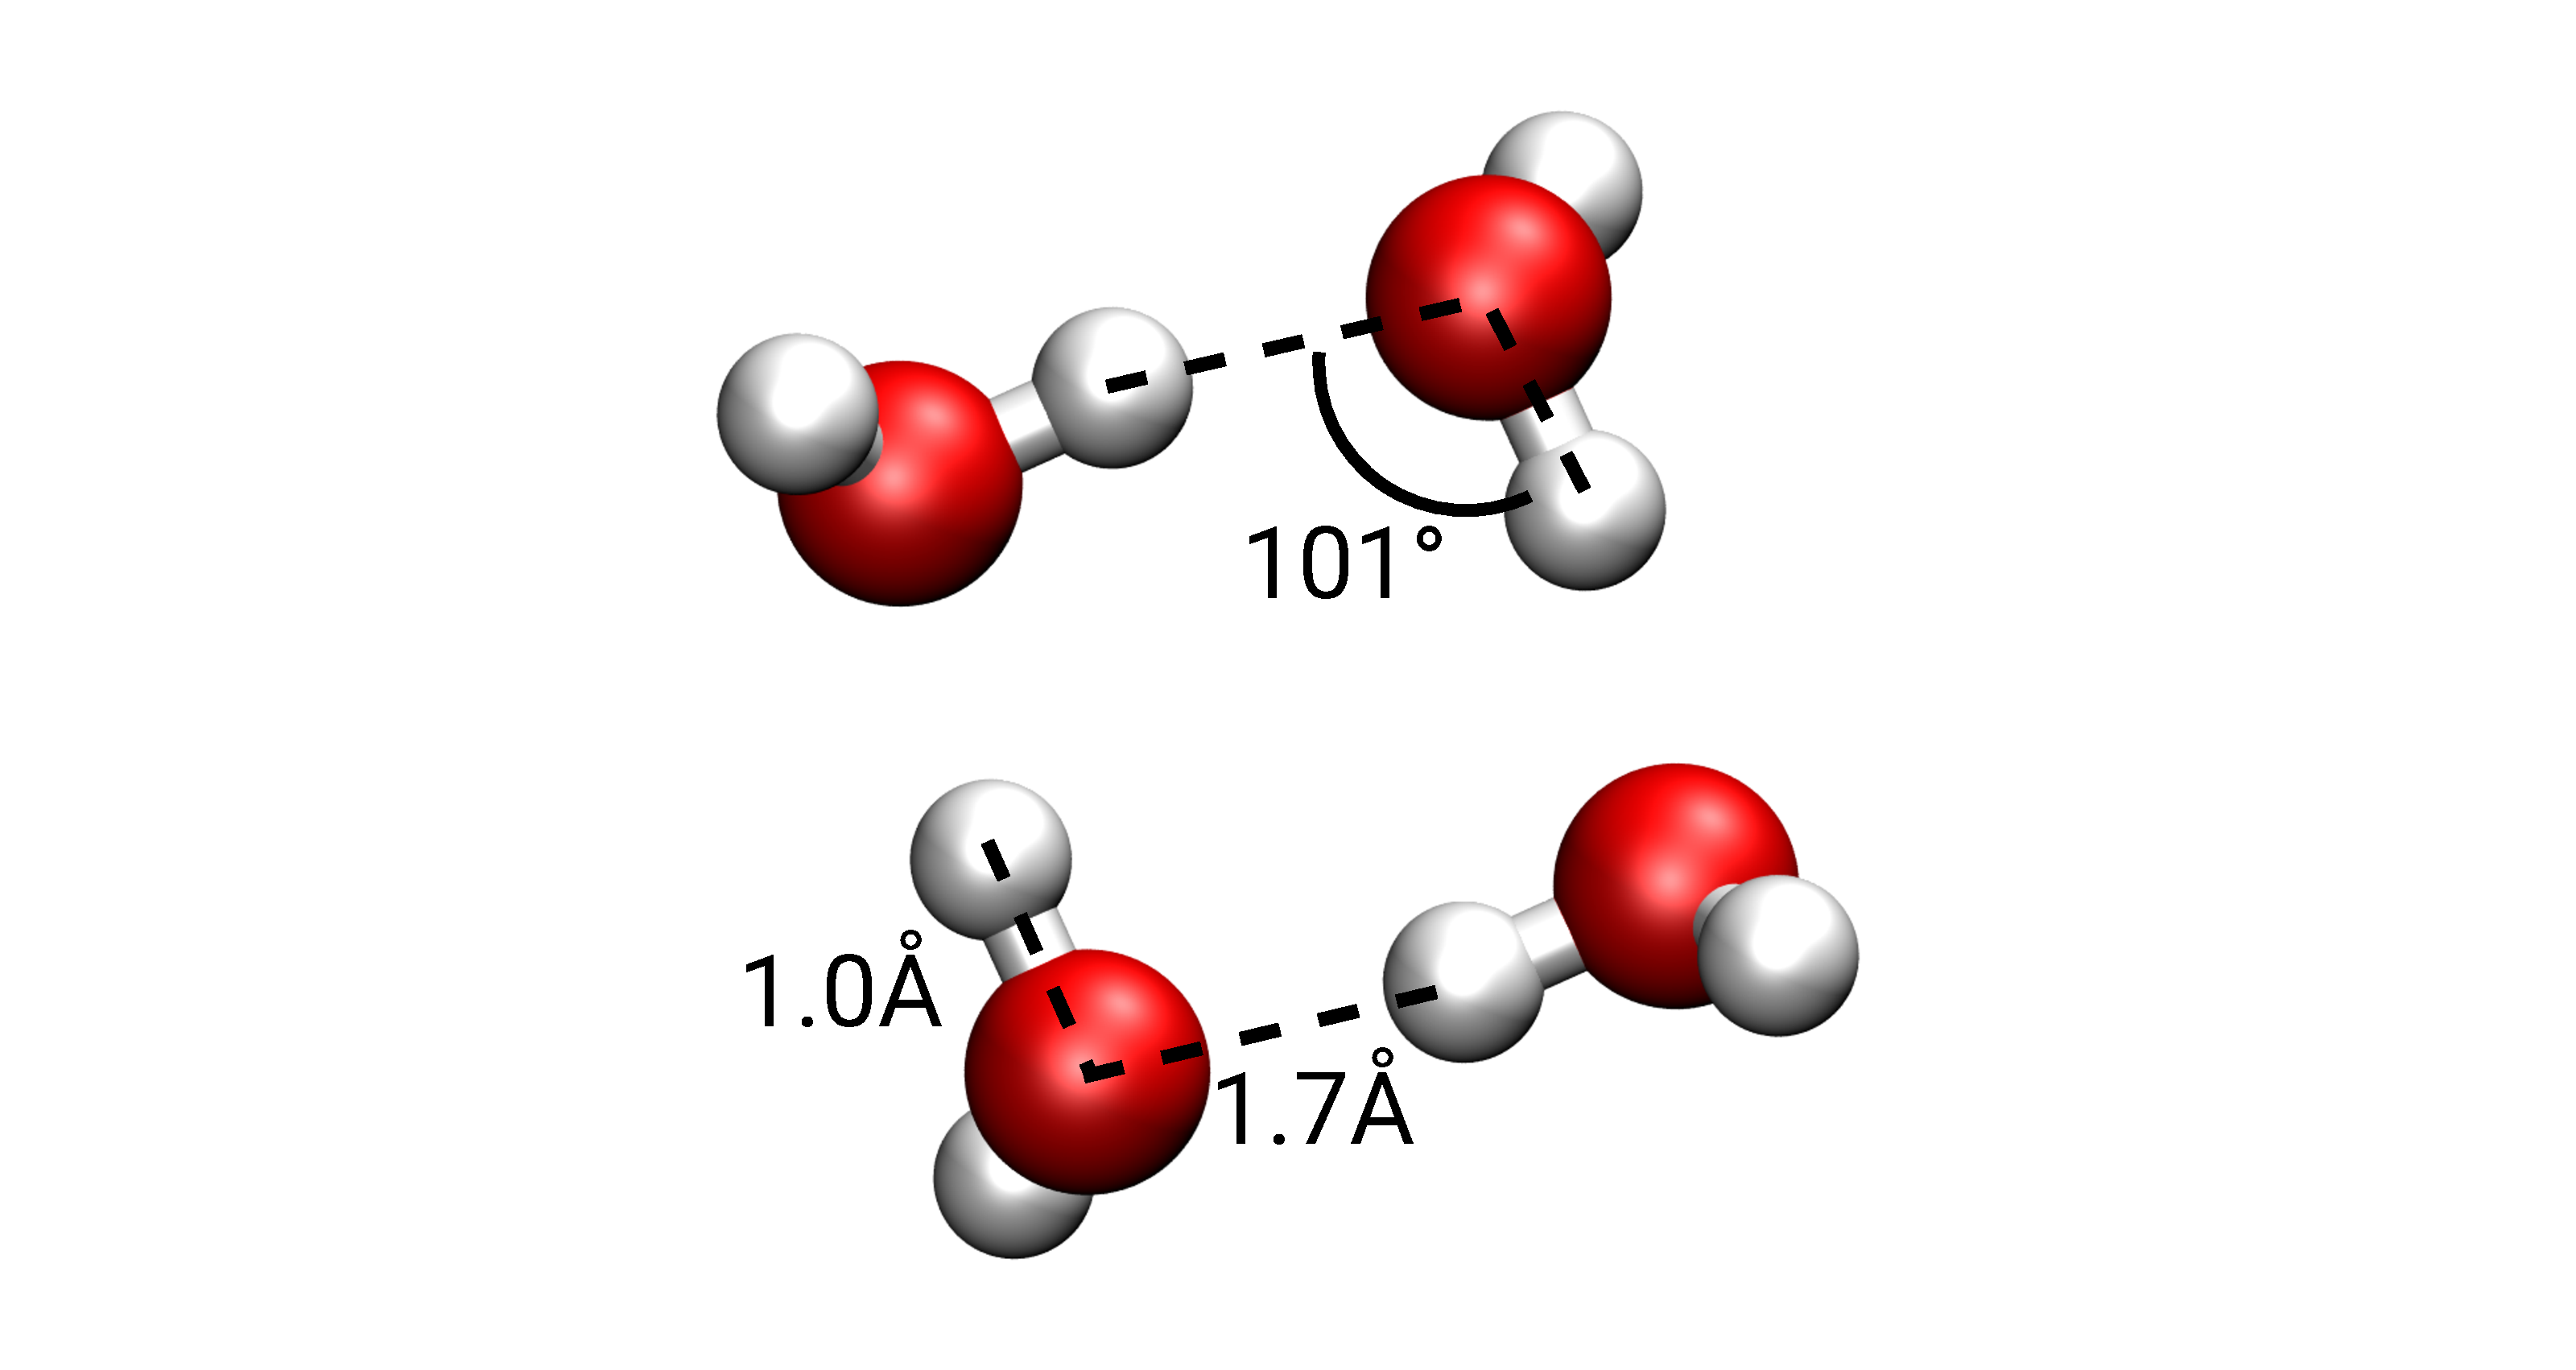
\includegraphics[width=.55\textwidth]{figures/0001/4H2O.pdf}}
  \quad
\subfigure[Coordinate system]{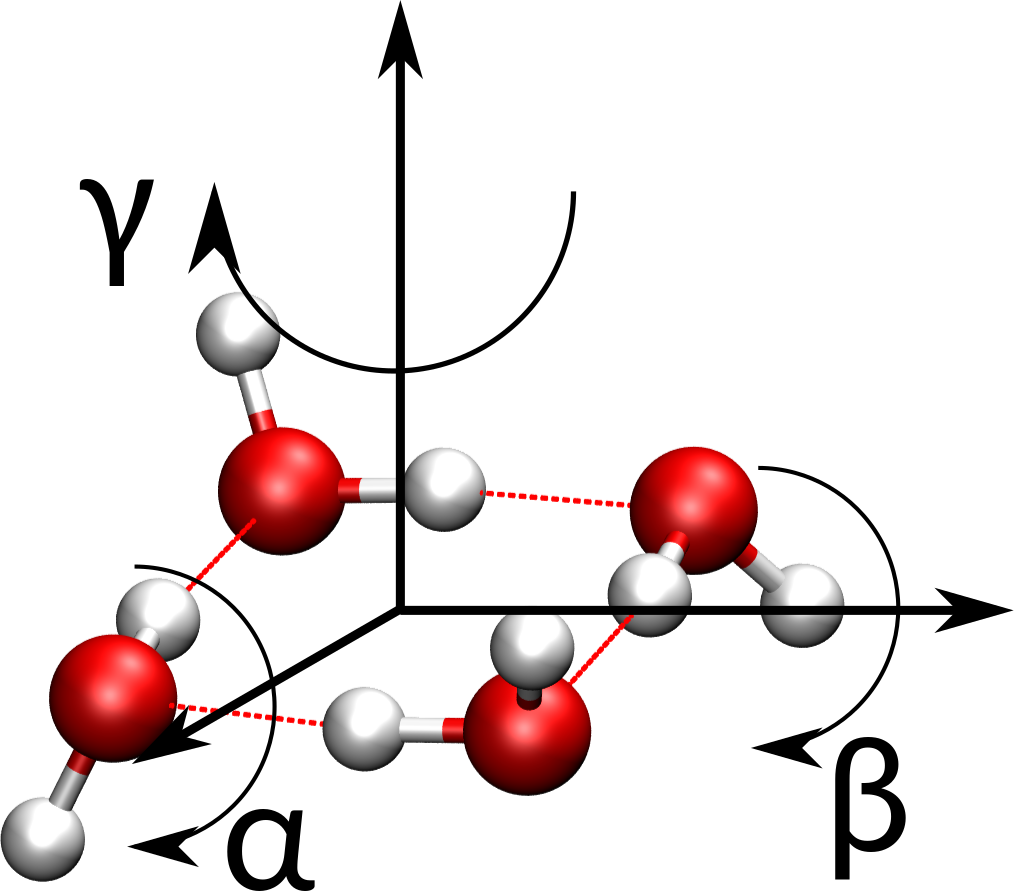
\includegraphics[width=.35\textwidth]{figures/0001/4d2o_axes.png}}
\caption{(D$_2$O)$_4$ cluster for simulation of effects of higher coverages.
(a) shows the optimized geometry, explaining the DOD bond angle and the OD bond lengths and (b) illustrates the coordinate system for the rotations along the axes with the angles $\upalpha$, $\beta$ and $\gamma$.}
       \label{abb:D2Ocluster}
\end{figure*}
Evaluating the data shows that the cluster breaks up upon contact with the surface into individual D$_2$O molecules and these undergo different processes, to a great extent influenced by the surrounding water molecules, due to the high coverage of $1\,$ML (the ($2\times 2$) supercell with its four CUS positions can hold up to four water molecules in one monolayer).
The water can adsorb molecularly or dissociatively (both directly and indirectly), physisorb, deuterium atoms can diffuse or single molecules can be reflected totally.
Two examples of the final geometries can be found in Figure \ref{abb:tetramer_traj}.
\begin{figure}[!ht]
\centering
\subfigure[]{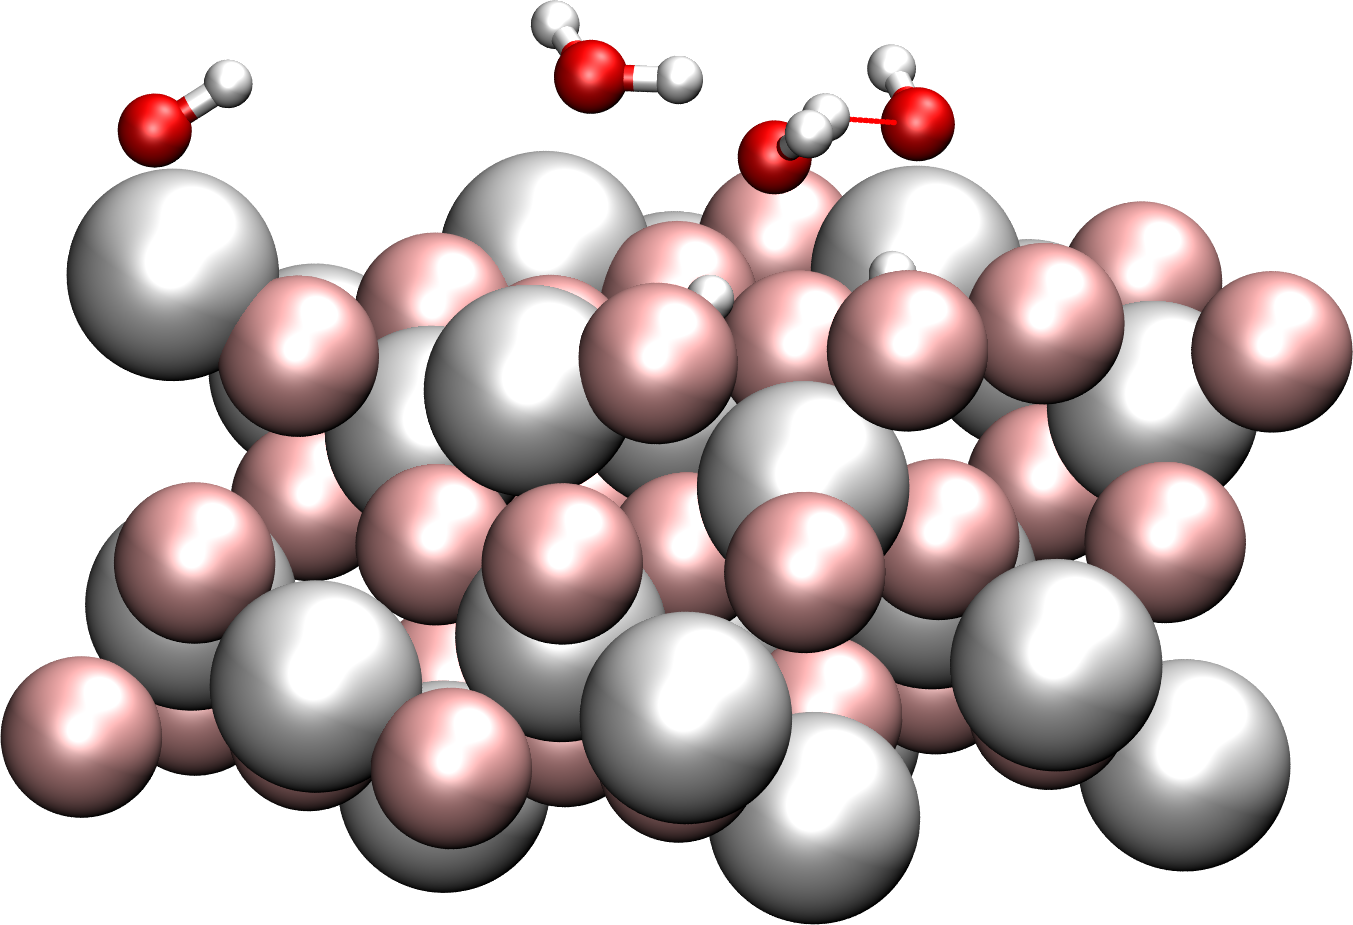
\includegraphics[angle=0,width=0.33\textwidth]{figures/0001/4d2o_05_035_000.png}} 
\quad
\subfigure[]{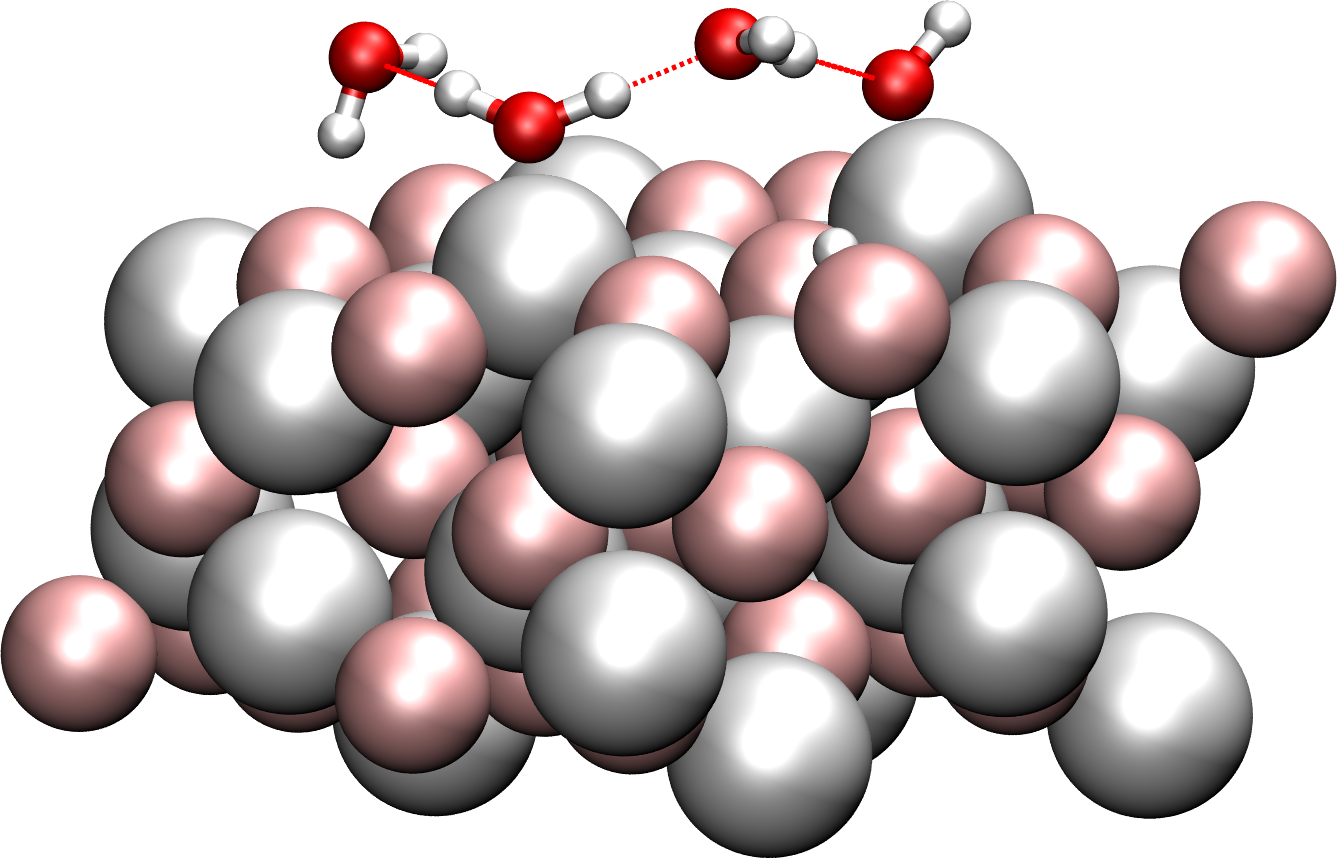
\includegraphics[width=0.33\textwidth]{figures/0001/4d2o_035_05_90900.png}}
\caption{Side views of the last time step ($1.22\,$ps) for two initial conditions: (a) E$_\textrm{kin}=0.9\,$eV, $[a_0,b_0]=[0.5,0.35]$, and $[\alpha,\beta,\gamma]=[0,0,0]$ and (b)  $E_\textrm{kin}=0.9\,$eV, $[a_0,b_0]=[0.35,0.5]$, 
 and $[\alpha,\beta,\gamma]=[90,90,0]$.
Hydrogen bonds are shown as red dashed lines.
Physisorption, molecular adsorption and dissociation can be seen in both snapshots.}
\label{abb:tetramer_traj}
\end{figure}
\\

Mostly independent of the settings, the molecules interact strongly with each other showing a profoundly dynamic behavior.
This gives rise to processes that were not possible for the clean surface NVE and a single water situation, where no 1-4 dissociation nor physisorption were observed.
Of course, the probabilities for dissociation, molecular adsorption and reflection are different, the probability of molecular adsorption is strongly diminished to the advance of 1-2, 1-4 and 1-4$^\prime$ dissociation and physisorption.
For details see Appendix \ref{reactionprobabilities}.

\subsubsection{Rotationally and Vibrationally Preexcited Water}\label{preex}
Qualitative results are given for a D$_2$O molecule which is not cold as before but excited rotationally and/or vibrationally at the beginning of the trajectory.
It is shot with a kinetic energy of $0.7\,$eV at the clean surface in an NVE ensemble for a trajectory duration of $2\,$ps at the impact point [$0.35,0.5$] with the initial orientation [$0,0,0$].
With these applied conditions in the ``cold'' case (microcanonical ensemble at $0\,$K without rotational or vibrational excitation), the molecule dissociates to the 1-2 structure, the same for the thermalized surface at $T=300\,$K.


The vibrational excitations were chosen as follows: For the single water molecule in the periodic boundary conditions a normal mode analysis was executed.
The eigenvectors of the dynamical matrix for the symmetric stretch, asymmetric stretch and the bending mode were used: The eigenvectors of the dynamical matrix equal normal mode displacements.
They were scaled by a factor of 0.1 and these positions were used as initial positions for the dynamics, giving a vibrational energy of around $0.05\,$eV. %\todo{E of first step of the trajecotry with vibration - E of trajectory's first step without vibration}
This corresponds to an atom displacement along normal modes out of the equilibrium position, \textit{i.e.}, a vibrational excitation.
It was used as an input for the MD trajectories in addition to the initial momentum towards the surface.
For the rotational preexcitations along the three axes, D atoms were given initial momenta to induce a rotational motion corresponding to rotational energies of $\sim$0.2$\,$eV.


The results for the rotation around the $\gamma$-axis (\textit{cf.} Figure \ref{abb:initial_parameters}) shows molecular adsorption whereas rotations around the other two axes give 1-2 dissociation as in the initial microcanonical trajectories without rotational excitation.
In the cases of vibrational preexcitation, the symmetric stretch leads to reflection, the asymmetric stretch gives 1-4$^\prime$ dissociation after initial 1-2 dissociation (as was already addressed in Figure \ref{abb:ex_traj}(d)) and with the bending mode being excited, the water dissociates to 1-2.
Also, a small collection of combinations of vibrations with rotations were calculated that lead to either molecular adsorption (rotation around $\alpha$ and bending mode), or 1-2 dissociation (rotation around $\gamma$ and asymmetric stretch; rotation around $\beta$ and symmetric stretch).


Quantitatively, the results may depend strongly on the excitation energy which was not of concern here, one can say that preexcitation has an effect on the dynamics of the water adsorption and dissociation, respectively that were not possible with the cold water molecule.
\\


In this section, AIMD calculations were done to model molecular beam scattering of heavy water on an $\upalpha$-Al$_2$O$_3$(0001) surface.
In respective experiments, molecular and dissociative adsorption has be observed, the latter in the form of modes of the 1-2, 1-4 and 1-4$^\prime$ dissociated species, with a much higher dissociation probability than in pinhole dosing.

In the simplest model, where a single D$_2$O molecule approaches the cold, clean surface, we find reflection, molecular adsorption and 1-2 dissociation only.
For dissociation, a minimum translational energy of the incoming molecule seems to be required, which may already be a hint to the fact why under MBS conditions dissociation is facilitated compared to pinhole dosing.

To find the experimentally verified 1-4 and 1-4$^\prime$ dissociated species, at least one of the following conditions has to be fulfilled:
A thermal surface (here $300\,$K), the preadsorption with molecular or dissociated water, the formation of water clusters in the beam, and the internal excitation (rotational or vibrational) of the incoming water molecules.

Apart from the mentioned processes, we have observed other channels and phenomena such as clustering of water (fragments) on the surface by H-bonding, chemisorption and physisorption, diffusion of water fragments, and collision induced chemical reactions, \textit{e.g.}, dissociation of adsorbed molecular water by the incoming D$_2$O molecule.

A rich chemistry evolves already on the ps time scale under more complex and realistic conditions.
The aforementioned processes can be direct or indirect, \textit{i.e.}, via (multiple) bounces at the surface or by sequences of reactions in which certain species appear as short-lived intermediates.

The main focus of this work was the qualitative analysis of water scattering at the $\upalpha$-Al$_2$O$_3$(0001) surface under increasingly complex conditions.
However, also semi-quantitative analyses were carried out, notably for the relative occurrence of the different products under different initial conditions.
We could find dependencies on the initial translational energy, rotational orientation, but even more on the impact site.
Also, dissociation is strongly favored when the incoming molecule hits the surface already in a ``product-like'' configuration.
These findings were published in Reference \cite{Heiden0001_2018}.


Although a large number of trajectories were computed with the contingent at the HLRN facility, a reliable statistical analysis was not possible.
Also some parameters (\textit{e.g.} different angles under which the beam hits the surface) have not been studied, and quantum effects were not considered.
The dynamics were restricted to the ps time scale.
%It was only computationally feasible to examine trajectories with $1$ to $4\,$ps duration.
%Due to the computational cost, only a limited set of degrees of freedom could be probed, \textit{e.g.} the angle of the beam with respect to the surface was no other than 90\textdegree{}, initial orientations were only probed in 90\textdegree{} steps and impact points were only considered for special points at the surface.
% Apart from that, no quantum effects were considered.
\clearpage

%%%%%%%%%%%%%%%%%%%%%%%%%%%%%%%%%%%%%%%%%%%%%%
\chapter[Water on $\upalpha$-Al$_2$O$_3$(11\=20)]{Water on $\upalpha$-Al$_2$O$_3$(11\=20)\cite{Heiden11-20_2018}}\label{sec:11-20}

The (11\=20) surface of $\upalpha$-Al$_2$O$_3$ is the third most stable one under UHV conditions and was not studied extensively so far, as discussed in the introduction.
Until now only a few experimental studies were performed for the (11\=20) surface: X-ray reflectivity measurements by J. Catalano\cite{catalano}, who found that the surface is oxygen terminated and has two differently coordinated kinds of surface Al atom dimers (groups of two Al atoms that form dimers by the reconstruction of the surface).
LEED measurements by Becker \textit{et al.}\cite{Becker2002} showed a well defined ($1\times 1$) diffraction pattern and found evidence that the surface is unreactive with hydrogen at room temperature.
The theoretical work of Marmier\cite{marmier} suggested that hydrogen is unreactive because the surface is fully hydroxylated at room temperature, even under UHV conditions.
In the work of Waychunas and coworkers\cite{sung}, SFG spectra were measured under ambient conditions (room temperature and air).
They found two different types of oxygen atoms on the surface, twofold and threefold coordinated ones.
The authors assumed that the threefold coordinated O will only be protonated under highly acidic conditions.
They also gave evidence for molecularly adsorbed water on the surface.
However, all experimental studies\cite{catalano,sung,Becker2002} assume a high-coverage situation, whereas this theoretical study is mostly focused on the low-coverage regime.
With theoretical methods, so far only the clean surface was studied by two different groups: Kurita \textit{et al.}\cite{kuri10} and Marmier\cite{marmier}.
Both papers disagree concerning the stability, in the work of Kurita, the (11\=20) surface is the third most stable surface cut, whereas in the publication of Marmier, it is the fourth most stable cut.

In this work we want to relate to SFG results for low-coverage experiments conducted by the Campen group from FHI Berlin, and to study reactivity of water at (11\=20) surface. %\todo{in comparison to (0001)}.
\section{Surface Models}
Our studies were done for a slab model of the O-I terminated (11\=20) surface, which was found to be the most stable one of five possible terminations in the theoretical work of Kurita \textit{et al.}\cite{kuri10}.
This is a stoichiometric, oxygen-terminated surface that is lower in energy than any other Al- or O-terminated (11\=20) surface.
In Section \ref{O-II-term} the less stable O-II termination is also studied to account for a defect site.

To allow for low water coverages, a ($2\times 2$) supercell was cut from the bulk.
In Figure \ref{abb:crystal_11-20}(a), the (11\=20) surface plane and the (0001) surface which was studied earlier in this work (Section \ref{sec:0001}) can be seen.
\begin{figure}[!h]
    \centering
    \subfigure[$\upalpha$-Al$_2$O$_3$ crystal cuts]{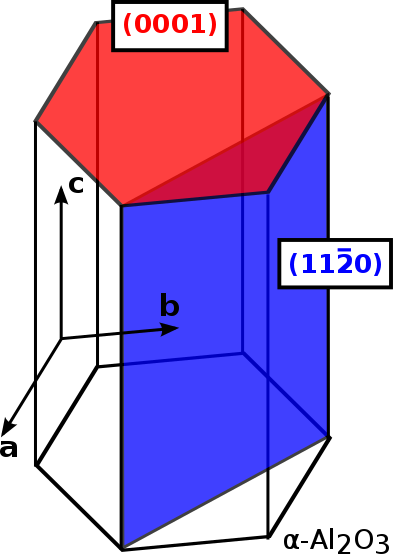
\includegraphics[width=0.30\textwidth]{figures/theory/al2o3-crystal.png}}
             \quad
             %add desired spacing between images, e. g. ~, \quad, \qquad, \hfill etc. (or a blank line to force the subfigure onto a new line)
    \subfigure[(11\=20), top view]{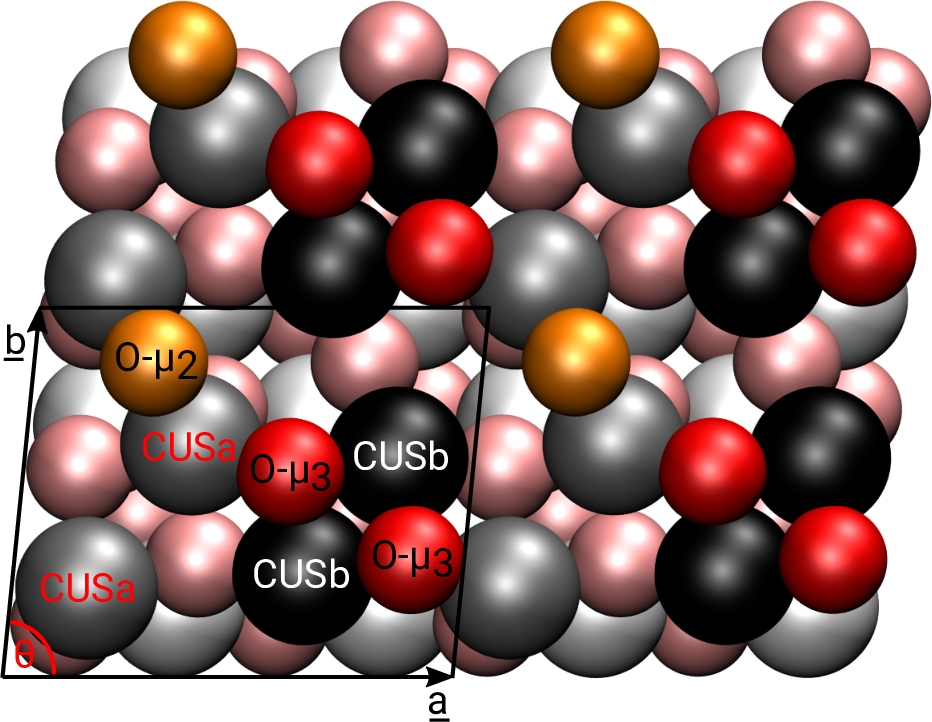
\includegraphics[width=0.58\textwidth]{figures/11-20/supercell_opt.png}}
             \quad
             %add desired spacing between images, e. g. ~, \quad, \qquad, \hfill etc. (or a blank line to force the subfigure onto a new line)
    \subfigure[(11\=20), side view]{\includegraphics[width=0.5\textwidth]{figures/11-20/uc_opt.png}}
             \caption{The (11\=20) surface cut of $\upalpha$-Al$_2$O$_3$, (a) schematic view of the Al$_2$O$_3$ crystal, where both the (0001) and the (11\=20) surface are shown, (b) a top view of the geometry optimized ($2\times 2$) supercell of (11\=20) of the most stable O-I termination, with the nomenclature of the surface atoms used in this work.
We distinguish two types of surface Al atoms (gray CUSa and black CUSb, where CUS is the abbreviation for coordinatively unsaturated site) as well as the twofold and threefold coordinated oxygen atoms (orange O-$\mu_2$ and red O-$\mu_3$).
Subsurface atoms are indicated by pale colors.
(c) gives the side view, for convenience of the ($1\times 1$) cell, showing the distinct atomic layers, again with the same color code as in (b).
The atoms below the solid line (the lowest five from ten layers) were fixed to bulk coordinates for optimizations and frequency analyses.
}
            \label{abb:crystal_11-20}
\end{figure}
In Figure \ref{abb:crystal_11-20}(b) the top view is shown and Figure \ref{abb:crystal_11-20}(c) gives the side view and the atomic layer sequence O-O$_2$-Al$_4$-O$_2$-O$\ldots$ for the ($1\times 1$) cell which is O$_4$-O$_8$-Al$_{16}$-O$_8$-O$_4\ldots$, respectively for the ($2\times 2$) cell that was applied in this work.
The supercell model that is mostly used in this work has ten atomic layers (two times this layer sequence, 32 Al and 48 O atoms), with the lowest five fixed to the bulk value to mimic the surface situation.
However, for the calculations of the lattice vibrations up to 30 layers were considered (in steps of five, see Figure \ref{abb:cell_sizes}).
For each system size, the lowest five layers were fixed (to the bulk values optimized with PBE+D2/PW).
The largest system (30 layers) was only used for one MD calculation due to its high computational effort, so in most cases the maximum layer thickness was 25.
\begin{figure}[!h]
    \centering
    \includegraphics[width=0.90\textwidth]{figures/11-20/cell_sizes.pdf}
             \caption{Side view for the different cell sizes for 10, 15, 20, 25 and 30 layers in z-direction.
Surface atoms are shown in the color code clarified before.
For each model size, the lowest five layers were kept fixed to bulk values.}
            \label{abb:cell_sizes}
\end{figure}

For the ($2\times 2$) supercell with the 10 layer system $\vec{k}$-points were sampled for five different grid sizes from ($1\times 1\times 1$) to ($5\times 5\times 1$) Monkhorst-Pack grids \cite{monkhorst}.
In contrast to the even grid sizes, the odd ones contain the $\Gamma$-point and therefore are favorable.
It can be deduced from Figure \ref{abb:11-20-kpointsampling} that the ($3\times 3\times 1$) grid is already converged with respect to the energy of the clean surface and will be used for all further calculations.
\begin{figure}[!h]
\centering
 \includegraphics[width=0.7\textwidth]{figures/11-20/irreducibles-E.eps}
   \caption{PBE+D2 energies for the clean surface (10 layer slab) as a function of the number of $\vec{k}$-points. Shown is the energy of the optimized supercell with respect to the number of $\vec{k}$-points in the irreducible part of the first Brillouin zone.
The even values correspond to the ($2\times 2 \times 1$) (2 $\vec{k}$-points in the irreducible part of the first Brillouin zone) and ($4\times 4\times 1$) (8), whereas the odd, which contain the $\Gamma$-point, are described by ($1\times 1\times 1$) (1), ($3\times 3\times 1$) (5) and ($5\times 5\times 1$) (13).}
            \label{abb:11-20-kpointsampling}
\end{figure}

The unit cell has a topmost layer of oxygen (O layer) in which each O atom is coordinated to two Al atoms of the underlying lattice.
Below this layer is a second oxygen layer (O$_2$ in Figure \ref{abb:crystal_11-20}(c)).
These O atoms are threefold coordinated by Al atoms.
Following the usual nomenclature in coordination chemistry, the two types of O atoms are denoted as O-$\mu_2$ and O-$\mu_3$, respectively.
In previous studies these have also been described as Al$_2$O and Al$_3$O\cite{sung}.
Below these surface oxygen layers is a layer of surface Al atoms (Al$_4$, consisting of four Al atoms in the ($1\times 1$) cell).
Within this Al layer there are two different coordinatively unsaturated (CUS) Al atoms, called here CUSa and CUSb, respectively.
By inspecting Figure \ref{abb:crystal_11-20}(b) it may become clear that CUSa Al atoms are covalently bound to one O-$\mu_2$, one O-$\mu_3$ and three deeper lying oxygen atoms, while CUSb atoms are covalently bound to two O-$\mu_3$ and three deeper lying oxygens.
In this work, the gray spheres denote the CUSa atoms, the black ones depict the CUSb atoms.
The twofold coordinated oxygen atoms (O-$\mu_2$) are shown in orange and the threefold coordinated (O-$\mu_3$) in red.
Atoms of the underlying layers are illustrated in pale colors, light gray for alumina and pale red for oxygen.
% The nomenclature and color code of the surface Al and O atoms is also shown in Figure \ref{abb:crystal_11-20}(b): The two types of aluminum atoms are coordinated by the same number of oxygen neighbor atoms but they differ slightly in the arrangement of their neighbors, %and the distance in the relaxed structure,
% whereas the two types of oxygen atoms in fact differ by the number of neighbors.
% The uppermost Al atoms are unsaturated and referred to as coordinatively unsaturates sites (CUS).
% In this work, the gray spheres denote the CUSa atoms, the black ones depict the CUSb.
% The twofold coordinated oxygen atoms (O-$\mu_2$) are shown in orange and the threefold coordinated (O-$\mu_3$) in red.
% Atoms of the underlying layers are illustrated in pale colors, light gray for alumina and pale red for oxygen.
% The unreconstructed unit cell consists of five mobile atomic layers in z-direction (O-O$_2$-Al$_4$-O$_2$-O), see Figure \ref{abb:crystal_11-20}(c)).

In the upper three layers of the ($2\times 2$) cell, we have 16 CUS sites (eight CUSa and eight CUSb), four O-$\mu_2$ and eight O-$\mu_3$ sites.
The corresponding cell vectors $\vec{a}$ and $\vec{b}$ were adopted from the bulk structure.
% Figure \ref{abb:crystal_11-20}(b) shows the top view of the ($2\times 2$) cell and the cell vectors $\vec{a}$ and $\vec{b}$ of (11\=20).
These are for this particular surface cut $|\vec{a}|=10.36\,$\AA, $|\vec{b}|=14.16\,$\AA{} and for the vector $\vec{c}$ perpendicular to the surface a length of $|\vec{c}|=20.5\,$\AA{} was assumed.
The angle $\theta$ between $\vec{a}$ and $\vec{b}$ is $84.56$\textdegree{}.

For the supercell model, a vacuum gap in z-direction (perpendicular to the surface, $17$\AA{} for the 10 layer slab, 15\AA{}, 13\AA{}, 11\AA{} and 9\AA{} for the 15, 20, 25 and 30 layer slabs, respectively) was introduced to avoid spurious, unphysical interaction between the slabs in this direction.

The spacing between the five top layers for each slab size is also displayed in Table \ref{tab:layer-dist}.
Upon relaxation the spacing between these layers is slightly changed compared to the bulk crystal as given in Table \ref{tab:layer-dist}.
The uppermost layer distance increases while it decreases for the deeper ones.
\begin{table}[!ht]
  \centering
 \caption{Distances between the top five layers (see also numbering in Figure \ref{abb:crystal_11-20}(c)) for different PBE+D2 optimized slab sizes (($3\times 3\times 1$) $\vec{k}$-point grid) and the unrelaxed bulk structure (right column) from theory.
All values are given in \AA.} 
\vspace*{.2cm}
\begin{tabular}{c|cccc|c}
\toprule
 & &\multicolumn{2}{c}{atomic layers}&&\\
    distance    & 10   & 15   & 20   & 25   &bulk \\\midrule
 d$_{12}$	&0.23 &0.23 &0.25 &0.25 &0.19 \\
 d$_{23}$	&0.64 &0.65 &0.64 &0.64 &0.74 \\
 d$_{34}$	&0.66 &0.66 &0.67 &0.67 &0.74 \\
 d$_{45}$	&0.20 &0.21 &0.21 &0.21 &0.19 \\\bottomrule
%     distance    & 10   & 15   & 20   & 25   &bulk \\\midrule
%  d$_{12}$	&0.232 &0.234 &0.247 &0.245 &0.193 \\
%  d$_{23}$	&0.642 &0.649 &0.638 &0.639 &0.741 \\
%  d$_{34}$	&0.656 &0.655 &0.671 &0.672 &0.741 \\
%  d$_{45}$	&0.198 &0.205 &0.209 &0.213 &0.191 \\\bottomrule
  \end{tabular}
  \label{tab:layer-dist}
\end{table}
A major issue of the optimization apart from layer spacing is that the interatomic distances of surface Al species change, here exemplarily for the 10 layer slab: the CUSa\textendash CUSa distance increases from $2.682$ to $2.994\,$\AA{}, the CUSa\textendash CUSb distance increases from $2.833$ to $2.876\,$\AA{} whereas the CUSb\textendash CUSb distance decreases from $2.682$ to $2.499\,$\AA{}.
The pairs of CUSa and CUSb can be interpreted as the Al dimers in the work of Catalano\cite{catalano}.




\section{Water Adsorption: Adsorption Energies and Geometries}\label{structure_search11-20}
\subsection{Low Coverage}
After optimization of the UHV surface termination, in a next step, water adsorption on the 10 layer relaxed (11\=20) surface model was studied, using PBE+D2, and the same computational parameters as above.
To study water adsorption, first a low-coverage regime was investigated: One water molecule per ($2\times 2$) supercell, which equals a coverage of 1/12\footnote{There are 16 CUS sites per ($2\times 2$) supercell, but adsorption does not occur on CUSa but only at a position between two CUSa atoms, which gives a maximum of 12 adsorption sites for 1 monolayer. See also Section \ref{sec:high_cov-ads}.}$^,$\footnote{Tests with a symmetric slab (where at the top and the bottom water is adsorbed) were computed, confirming that the asymmetric model (water is only adsorbed on one side of the slab) including dipole corrections is sufficient to describe the system.
% Only minor differences could be obtained.
Details for this are given in Appendix \ref{symmetric_slab}.}.
For this a water molecule was put at different positions on the surface and the system was relaxed.
By doing so one molecular minimum and several dissociated species including both CUS and oxygen types were found.
The multitude of different surface atoms gives rise, for the dissociated water molecule, to a large variety of possible adsorption geometries for the next neighboring situation (OH and H residue are adsorbed on two neighboring surface atoms).
The variety is even increased when considering adsorbate structures with greater distance between the dissociated water fragments.
Adsorption energies and Gibbs free energies at various temperatures of the resulting, dissociated next neighbor species can be seen in Table \ref{tab:ads_1water}, along with the molecular species (see also Figure \ref{abb:ads-geoms}).
The adsorption energy is defined (analogously to Equation (\ref{eq:Eads1}) in Section \ref{sec:0001}) as the energy of the adsorbed species compared to the energies of the clean surface and the free water molecule.
% \begin{equation}\label{eq:Eads}
%  E_\textrm{ads}=E_\textrm{ads. species}-(E_\text{free water molecule}+E_\text{surface}).
% \end{equation}
The nomenclature for the adsorption sites which is used in the following gives at first the type of Al site where the OH residue (or OH$^-$) is adsorbed and at second place the oxygen type where the H (H$^+$) is adsorbed: OH site$\parallel$H site.
The term ``inter'' characterizes a position between two CUS atoms which leads to a bidentate adsorption pattern.
The additional notation with $^\prime$ denotes greater distances between the residues.
Direct neighbors do not have a $^\prime$, the next neighbor structure is displayed by a single $^\prime$, one position farther $^{\prime\prime}$ and the most distant position is $^{\prime\prime\prime}$ due to the periodic boundary conditions.
% There is also one metastable molecular species that appears to be more stable than the found molecular minimum considering adsorption energy, but it cannot be classified as a stable minimum since there is one imaginary mode displaying the movement of the proton towards the dissociated species.



\begin{table}[!ht]
  \centering
 \caption{For molecular and (singly) dissociated water on a ($2\times 2$) cell of $\upalpha$-Al$_2$O$_3$(11\=20), adsorption energies E$_\textrm{ads}$ and Gibbs free energies $G_\textrm{ads}$ for different temperatures for the 10 layer slab are given in eV.
E$_\textrm{ads}$ was calculated from Equation (\ref{eq:Eads1}) and G$_\textrm{ads}$ is defined analogously.
These results were obtained with PBE+D2.
The three most stable species are marked with bold letters.
\vspace*{.2cm} 
  }
  \begin{tabular}{cl|cccc}
  \toprule
   \multicolumn{2}{c|}{Adsorbed Species}  & $E_\textrm{ads}$ & $G_\text{ads, 130 K}$  &  $G_\text{ads, 300 K}$  & $G_\text{ads, 400 K}$ \\\midrule
\multirow{1}{*}{molecular} & CUSb          &   -1.78  &-1.60 & -1.51  & -1.46 \\\hline
 \multirow{6}{*}{dissociated} & \textbf{inter-CUSa$\parallel$O-$\mu_2$} & \textbf{-2.50} &-2.27 & -2.16 & -2.09 \\
  & inter-CUSa$\parallel$O-$\mu_3$ & -1.67 &-1.44 &-1.33 & -1.27 \\
  & \textbf{CUSb$\parallel$O-$\mu_2$} & \textbf{-2.28} & -2.12& -2.03 &-1.97  \\
 & CUSb$\parallel$O-$\mu_3$ & -1.19 &-1.05 &-0.98 & -0.95 \\%Cb3_other
 & \textbf{inter-CUSb$\parallel$O-$\mu_2$} & \textbf{-2.09} &-1.88 &-1.80 & -1.76 \\
 & inter-CUSb$\parallel$O-$\mu_3$ & -1.89 &-1.71 & -1.63 & -1.58 \\\bottomrule
  \end{tabular}
  \label{tab:ads_1water}
\end{table}
\begin{figure}[!ht]
 \centering
\subfigure[CUSb]{\includegraphics[width=0.2\textwidth]{figures/11-20/test-Cb.pdf}}
 \quad\quad
 \subfigure[inter-CUSa$\parallel$O-$\mu_2$]{\includegraphics[width=0.2\textwidth]{figures/11-20/test-iCa2.pdf}}
  \quad
\subfigure[CUSb$\parallel$O-$\mu_2$]{\includegraphics[width=0.2\textwidth]{figures/11-20/test-Cb2.pdf}}
 \quad
\subfigure[inter-CUSb$\parallel$O-$\mu_2$]{\includegraphics[width=0.2\textwidth]{figures/11-20/test-iCb2.pdf}}
\quad
\subfigure[inter-CUSa$\parallel$O-$\mu_3$]{\includegraphics[width=0.2\textwidth]{figures/11-20/test-iCa3.pdf}}
 \quad
\subfigure[CUSb$\parallel$O-$\mu_3$]{\includegraphics[width=0.2\textwidth]{figures/11-20/test-Cb3.pdf}}
 \quad
\subfigure[inter-CUSb$\parallel$O-$\mu_3$]{\includegraphics[width=0.2\textwidth]{figures/11-20/test-iCb3.pdf}}
 \caption{Top view of the adsorption geometries for molecular CUSb (a) and the next neighbor dissociated water 
((b)-(g)).
The color code is the same as in Figure \ref{abb:crystal_11-20}(b) and (c), CUSa gray, CUSb black, O-$\mu_2$ orange and O-$\mu_3$ red; hydrogen is illustrated in white; the oxygen from water is in red but as a smaller sphere to make it distinguishable from the surface O atoms; subsurface layers are shown in pale colors.}
        \label{abb:ads-geoms}
 \end{figure}

Our structure search suggests that a single water molecule adsorbs with an adsorption energy of $-1.78\,$eV on CUSb.
Molecular adsorption between two CUSa (inter-CUSa) or between to CUSb (inter-CUSb) does not occur at the level of theory employed here.
Geometries with starting conditions at these sites show dissociation.
The molecular minimum is substantially less stable than most of the dissociated species.
Also, we find that all six next neighbor combinations of OH$^-$ and H$^+$ sites are minima in our model.
On the contrary, the dissociated water, where the twofold coordinated surface oxygen atom is addressed, is very stable, even in comparison to the more stable surface cuts (0001) and (1\=102) that were previously investigated in our group in References\cite{Wirth2016,WirthJPCC2012}.
Dissociated species where the proton is located at a twofold coordinated surface oxygen are far more stable than the corresponding systems where the threefold coordinated oxygen is occupied.
This is due to the higher negative charge and the higher basicity of such twofold coordinated oxygen atoms O-$\mu_2$, in comparison with the more saturated threefold coordinated O-$\mu_3$ oxygen atom.
In fact, the adsorption can be seen as a Lewis acid / base reaction\cite{Stair1981} with the undercoordinated aluminum being the Lewis acid and the oxygen of the water molecule being the base.


The adsorption of OH at an inter-CUSa site is more favorable than at a CUSb site, because the former corresponds to a site where in the bulk system another oxygen atom would be situated, which is not the case for the CUSb position.
Additionally, the CUSb position is electronically\footnote{Two electron rich oxygen atoms are nearby, that also cause a repulsion by the elevated local negative charge.} and sterically more hindered because of the twofold and threefold coordinated oxygen atoms in the surroundings.


Dissociated species with fragments in direct neighborhood as shown in Table \ref{tab:ads_1water} and Figure \ref{abb:ads-geoms} are more stable than those where the proton and the OH residue are farther apart (see Table \ref{tab:ads_1waterfurther}), given the OH residue has a stabilizing effect on the H and vice versa.
What first seems to disagree with the former said is that the inter-CUSb$\parallel$O-$\mu_3^{\prime\prime\prime}$-species is more stable than the species inter-CUSb$\parallel$O-$\mu_3^{\prime\prime}$ (where the OH groups are closer to each other).
However, this is due to the fact that in the unit cell the fragments of inter-CUSb$\parallel$O-$\mu_3^{\prime\prime}$ are closer but in the periodic boundary conditions actually the distance between OH and H in inter-CUSb$\parallel$O-$\mu_3^{\prime\prime\prime}$ is smaller.
The distances between the neighboring OH groups in the O-$\mu_3^{\prime\prime}$ system are $6.76$ and $7.71\,$\AA{}, compared to $9.34$ and $6.16\,$\AA{} in the O-$\mu_3^{\prime\prime\prime}$ system (the numbers refer to the two possible distances in the periodic system, direct and ``over the border'' of the unit cell).
The latter seems to be farther away, but due to the periodic boundary conditions, one of the inter-adsorbate distances is smaller ($6.16$, compared to $6.76\,$\AA{}), which leads to the stabilization.

%one is in fact only slightly further away, the average distance is $0.739\,$\AA{} for inter-CUSb$\parallel$O-$\mu_3^{\prime\prime}$ and $0.780\,$\AA{} for inter-CUSb$\parallel$O-$\mu_3^{\prime\prime\prime}$.
% Although the distance is larger, there seems to be more stabilization by the surrounding surface atoms.
% In Section \ref{reactions} dissociation and diffusion reactions will be given.
\begin{table}[!ht]
  \centering
 \caption{Comparison of adsorption energies for next neighbor dissociated species (without $^\prime$), and dissociated species where OH and H are farther apart (with one, two or three $^\prime$). 
Results are given in eV (10 layer slab).
\vspace*{.2cm} 
  }
  \begin{tabular}{cc}
  \toprule
  Adsorbed Species  & $E_\textrm{ads}$  \\\midrule
   inter-CUSa$\parallel$O-$\mu_3$ & -1.67 \\
   inter-CUSa$\parallel$O-$\mu_3^\prime$ & -1.42 \\\hline
   inter-CUSb$\parallel$O-$\mu_3$ & -1.89\\
   inter-CUSb$\parallel$O-$\mu_3^{\prime\prime}$ & -1.16\\
   inter-CUSb$\parallel$O-$\mu_3^{\prime\prime\prime}$ & -1.22\\\bottomrule
  \end{tabular}
  \label{tab:ads_1waterfurther}
\end{table}


Besides, water adsorption for systems with additional atomic layers (up to 25 in total) were studied to check convergence with respect to layer thickness.
These optimized geometries do not differ strongly from the 10 layer ones and hence are not shown.
The corresponding adsorption energies are shown in Table \ref{tab:eads_layers}.
The adsorption energies do not change largely with increasing slab size.
The molecular species still is less stable than the O-$\mu_2$ dissociated species and is more stable than the O-$\mu_3$ dissociated ones (except for inter-CUSb$\parallel$O-$\mu_3$ dissociated system).
inter-CUSa$\parallel$O-$\mu_2$ is the most stable structure for all sampled system sizes, inter-CUSb$\parallel$O-$\mu_2$ and CUSb$\parallel$O-$\mu_2$ change their stability (it approaches to nearly the same value for 25 layers) depending on the number of layers but still are some orders of magnitude less probable than inter-CUSa$\parallel$O-$\mu_2$\footnote{See discussion in Section \ref{nma-OD}.}.
Dissociated systems occupying the threefold coordinated surface oxygen atom remain in the same stability order.
%For higher quantity of layers, the inter-CUSb gets more favourable than CUSb, both for O-$\mu_2$ and O-$\mu_3$.
%This might be due to less interaction between neighboring oxygen atoms with the inter-CUSb adsorbed OH group.
\begin{table}[!ht]
  \centering
  \caption{Adsorption energies $E_\textrm{ads}$ calculated from Equation (\ref{eq:Eads1}) for molecular and dissociated species, as a function of layer thickness.
All values are given in eV.
The most stable systems (inter-CUSa$\parallel$O-$\mu_2$, CUSb$\parallel$O-$\mu_2$ and inter-CUSb$\parallel$O-$\mu_2$) are highlighted in bold letters.}
 \begin{tabular}{l|cccc}
 \toprule
 System                     & 10 layers& 15 layers& 20 layers& 25 layers \\\midrule
CUSb                                    &-1.78 &-1.80     &-1.81     &-1.83      \\\hline
\textbf{inter-CUSa$\parallel$O-$\mu_2$}    &\textbf{-2.50} &\textbf{-2.46} &\textbf{-2.54} &\textbf{-2.56}  \\
inter-CUSa$\parallel$O-$\mu_3$          &-1.67 &-1.67 &-1.78 &-1.80 \\
\textbf{CUSb$\parallel$O-$\mu_2$}          &\textbf{-2.28} &\textbf{-2.35} &\textbf{-2.36} &\textbf{-2.35} \\
CUSb$\parallel$O-$\mu_3$                &-1.19 &-1.71 &-     &-      \\
\textbf{inter-CUSb$\parallel$O-$\mu_2$}    &\textbf{-2.09} &\textbf{-2.43} &\textbf{-2.48} &\textbf{-2.36}  \\
inter-CUSb$\parallel$O-$\mu_3$          &-1.89 &-1.59 &-1.65 &-2.09 \\\bottomrule
\end{tabular}
\label{tab:eads_layers}
\end{table}
Table \ref{tab:eads_layers} shows that the most stable systems are already converged for the 10 layer slab with regard to adsorption energies (and also vibrational OD stretch frequencies as it will be seen in Section \ref{nma}).

\subsection{Higher Coverages}\label{sec:high_cov-ads}

Furthermore, systems with a higher water coverage were investigated, which offer the possibility to consider interaction between the adsorbate molecules.
For the ($2\times 2$) supercell approach of the clean surface there are 16 CUS Al-atoms.
% These have fewer bonds than the aluminum atoms in the bulk structure since the surface layer is depleted.
% These atoms are very interesting for adsorbate molecules/atoms, because these surface atoms are electron rich and can be addressed for adsorption.
Theoretically, these 16 atoms could be covered with water to gain 1 monolayer (ML).
Eight of these 16 CUS atoms are CUSa and eight CUSb.
On top of CUSb, a water molecule/OH residue can adsorb, but on top of a CUSa the adsorbate roams to a bridging inter-CUSa position between two CUSa.
Thus, the number of potential adsorbates is decreased to twelve forming 1ML.
Some exemplary cases for two water molecules (2/12=$16.6\%$ coverage), four inter-CUSa$\parallel$O-$\mu_2$ (4/12=$33.3\%$ coverage) and a fully covered supercell (twelve molecules, 12/12=$100\%$ coverage) within a ($2\times 2$) supercell 10 layer slab model are shown in Figures \ref{abb:2water} and \ref{abb:4+fully}.
For these systems also normal mode analyses were carried out to get vibrational spectra, see Section \ref{phonons} and Appendix \ref{app:11-20_freq_hig_cov+O-II}.
\begin{figure}[!ht]
 \centering
\subfigure[CUSb+CUSb$\parallel$O-$\mu_2$]{\includegraphics[width=0.302\textwidth]{figures/11-20/Cb-Cb2.png}}
 \quad\quad
 \subfigure[inter-CUSa$\parallel$O-$\mu_2$+CUSb$\parallel$O-$\mu_2$]{\includegraphics[width=0.304\textwidth]{figures/11-20/iCa2-Cb2.png}}
  \quad
\subfigure[2inter-CUSa$\parallel$O-$\mu_2$]{\includegraphics[width=0.302\textwidth]{figures/11-20/iCa2-iCa2.png}}
 \quad
 \caption{PBE+D2 optimized geometries of systems with two water adsorbates per ($2\times 2$) cell: (a) molecular CUSb and CUSb$\parallel$O-$\mu_2$, (b) the two most stable species inter-CUSa$\parallel$O-$\mu_2$ and CUSb$\parallel$O-$\mu_2$ and (c) 2inter-CUSa$\parallel$O-$\mu_2$.} %, which is the most stable adsorption pattern.}
        \label{abb:2water}
 \end{figure}
 \begin{figure}[!ht]
 \centering
\subfigure[4inter-CUSa$\parallel$O-$\mu_2$]{\includegraphics[width=0.4\textwidth]{figures/11-20/4iCa2.png}}
 \quad\quad
 \subfigure[1ML]{\includegraphics[width=0.4\textwidth]{figures/11-20/O-I-fully.png}}
 \caption{Optimized structures of the (a) 4inter-CUSa$\parallel$O-$\mu_2$ (four water molecules) and (b) fully covered (1ML) system (twelve water molecules).
The latter one shows one molecular species and several hydrogen-bonded OH groups.}
        \label{abb:4+fully}
 \end{figure}

The adsorption energy of species with $n$ adsorbed water molecules was calculated as
\begin{equation}\label{eq:eadshigh}
 E_\textrm{ads}=E_\textrm{ads. species}-(n\times E_\text{free water molecule}+E_\text{surface}).
\end{equation}
In Table \ref{tab:higher_water}, the adsorption energies for the high-coverage species mentioned above are given.
\begin{table}[!ht]
  \centering
 \caption{Adsorption energies $E_\textrm{ads}$ from Equation (\ref{eq:eadshigh}) for higher water coverages in eV.
For better comparison the adsorption energy per water molecule, the non-interacting adsorption energy from Equation (\ref{eq:eadsnoninteract}) and the stabilization energy $E_\textrm{stab.}$ from Equation (\ref{eq:stab}) are given.
Also the coverage and number of water molecules per cell can be found here.
% in the third column labeled ``isolated species'' the summed energies for singly adsorbed water as given in Table \ref{tab:ads_1water} are presented.
\vspace*{.2cm} 
  }
  \begin{tabular}{lcccccc}
  \toprule
  Adsorbed Species  & $E_\textrm{ads}$ & $E_\textrm{ads,non-int.}$& $E_\textrm{stab.}$& $\frac{E_\textrm{ads}}{n}$& Coverage &H$_2$O/cell \\\midrule
   CUSb(mol)+CUSb$\parallel$O-$\mu_2$ & -4.57 & -1.78+(-2.28)=-4.06&-0.51& -2.29&1/6&2\\
   inter-CUSa$\parallel$O-$\mu_2$+CUSb$\parallel$O-$\mu_2$ & -4.77 & -2.50+(-2.28)=-4.78&+0.01& -2.39& 1/6&2\\
   2inter-CUSa$\parallel$O-$\mu_2$& -4.84 &2$\times$(-2.50)=-5.00&+0.16& -2.42& 1/6&2 \\\hline
   4inter-CUSa$\parallel$O-$\mu_2$ & -9.55 & 4$\times$(-2.50)=-10.00&+0.45& -2.39& 1/3&4\\\hline
   12H$_2$O & -23.39& $^a$\tnote{a} &-& -1.95& 1/1& 12\\\bottomrule
  \end{tabular}
  \label{tab:higher_water}
  \begin{tablenotes}\footnotesize 
    \item[a] $^a$ In good approximation, there are 4 inter-CUSa-OH groups, 8 CUSb-OH groups, 8 O-$\mu_3$ and 4 O-$\mu_2$ OH groups, hence one can not calculate $E_\textrm{ads,non-int.}$.
  \end{tablenotes}
\end{table}
There are also the results for the higher coverages in comparison to results in the low-coverage limit presented by calculating the non-interacting adsorption energy with Equation (\ref{eq:eadsnoninteract}) (see also Table \ref{tab:higher_water})
\begin{equation}\label{eq:eadsnoninteract}
 E_\textrm{ads,non-int.}=E_\textrm{ads, species 1} + E_\textrm{ads, species 2}~,
\end{equation}
and with that the stabilizing energy $E_\textrm{stab.}$:
\begin{equation}\label{eq:stab}
 E_\textrm{stab.}=E_\textrm{ads}-E_\textrm{ads,non-int.}~.
\end{equation}

The structures were chosen exemplarily such that the neighborhood effect shows three different outcomes: it can have a stabilizing effect, where the dissociated water stabilizes the molecularly adsorbed water in CUSb(mol)+CUSb$\parallel$O-$\mu_2$ (Figure \ref{abb:2water}(a)).
It can also have the contrary effect, as can be seen in the  2inter-CUSa$\parallel$O-$\mu_2$, which becomes less stable (Figure \ref{abb:2water}(c)).
On the other hand, there is the inter-CUSa$\parallel$O-$\mu_2$+CUSb$\parallel$O-$\mu_2$, which is merely affected by the neighboring OH residues (Figure \ref{abb:2water}(b)).

\subsection{Other Surface Terminations}\label{O-II-term}
Up to this point, only the most stable O-I termination was considered.
% This subsection will deal with the O-II termination that is thermodynamically less stable and serves as a model for a defect surface, where the topmost oxygen atom is missing.

In experimental LEED data of the clean surface\cite{Heiden11-20_2018}, the analysis of the data gave two sublattices, one of them can be clearly identified as the most stable O-I termination and the other one remains unidentified.
This unknown lattice could be a defect surface or another surface termination but this suggestion could not be confirmed yet by experimental data since preparation and probing turns out to be difficult.
To pursue this thesis, a ``defect surface'', the O-II terminated surface, as it is called in the nomenclature of Kurita\cite{kuri10}, was calculated.
This is the second most stable surface termination under most chemical potential conditions, mostly in Al-rich environment.
In this termination, the topmost oxygen layer of the O-I termination is missing.
As for the O-I termination, ten layers were considered and from these the lowest five layers were kept fixed to bulk values.
Both the clean surface and one possible configuration of the fully covered ($1\,$ML) surface were optimized (see Figure \ref{abb:O-II-geom}) and frequency calculations were performed to obtain vibrational modes, see Appendix \ref{app:11-20_freq_hig_cov+O-II}.
The structure of the clean surface, of course, differs by the ``missing'' oxygen O-$\mu_2$ atoms in the topmost layer, and the fully covered system is even more different: out of twelve water molecules that can adsorb, seven adsorb molecularly and five dissociatively.
In comparison, the fully covered system for the O-I termination only shows one molecularly adsorbed molecule (\textit{cf.} Figure \ref{abb:4+fully}(b)).
 \begin{figure}[!ht]
 \centering
\subfigure[clean O-II surface]{\includegraphics[width=0.4\textwidth]{figures/11-20/O-II-clean.png}}
 \quad\quad
 \subfigure[fully covered O-II surface]{\includegraphics[width=0.4\textwidth]{figures/11-20/O-II-fully.png}}
 \caption{O-II terminated surface, as an example of a defect site optimized with PBE+D2.
The top layer oxygen atom from the O-I terminated surface is missing and gives rise to a different chemical behavior.
(a) clean surface, (b) 1ML water adsorbed surface.}
        \label{abb:O-II-geom}
 \end{figure}

\section{Dissociation and Diffusion Reactions of Water Species}\label{reactions}

Based on the minimum structures one has to identify reaction pathways linking these minima to fully understand the reactivity of a system.
We utilize the NEB method including climbing image to search for transition states between the minima of the 10 layer slab.
For coverage 1/12 (one molecule per ($2\times 2$) cell of the O-I terminated surface), we examined three different types of reactions: dissociation from the molecular minimum, as well as OH- and H-diffusion.
% These reaction paths and corresponding rates were calculated for hydrogen instead of deuterium that was used for vibrational frequencies since H$_2$O is more ubiquitous in nature (see Section \ref{sec:vib11-20}).
The dissociation reactions are named D, diffusion reactions as Df-OH and Df-H, respectively, in Table \ref{tab:reaction-rates} and Figures \ref{mep} and \ref{mep2}.
In addition, molecular water diffusion on the surface is supposable but due to the low stability, it will dissociate before diffusion can occur.
% In the publication that emerged from this work (Reference \cite{Heiden11-20_2018}) most of the reactions were introduced; additional reactions paths are also considered here.


We investigated two distinct dissociation reactions: the reactions from CUSb to the twofold coordinated oxygen (D-I) and one to the threefold coordinated O-$\mu_3$ (D-II).
% One additional dissociation starts from the metastable inter-CUSa molecular structure that is, as said before, no minimum structure and goes to the most stable species inter-CUSa$\parallel$O-$\mu_2$ (D-c).
% Two further dissociation reactions were converged but showed a two step process and are therefore not interesting in the first place (these reactions are CUSb$\rightarrow$inter-CUSa$\parallel$O-$\mu_2$ and CUSb$\rightarrow$inter-CUSb$\parallel$O-$\mu_2$ and both went via the dissociated CUSb$\parallel$O-$\mu_2$ intermediate).


As can be seen from Table \ref{tab:ads_1water} (Section \ref{structure_search11-20}), the molecular minimum CUSb has a lower stability compared to the O-$\mu_2$ dissociated minimum.
The reaction D-I leads from the molecular minimum at CUSb to the twofold coordinated oxygen of CUSb$\parallel$O-$\mu_2$:
 \begin{equation}
 \text{H$_2$O(CUSb)} \rightarrow \text{OH(CUSb)} + \text{H(O-$\mu_2$)}. \tag{D-I}
      \label{dissI}
\end{equation}
This reaction is very exoenergetic and exergonic.
The free energy barrier is very low, about $0.002\,$eV as one can see from Table \ref{tab:reaction-rates} and Figure \ref{mep}(a), hence the reaction rate constant is very high, in the order of $k(\textrm{300\,K})=5.76\times 10^{12}$s$^{-1}$.
This barrier is probably too low due to the underestimation of barrier heights\cite{Zhao05} with the used functional PBE. %(compare section \ref{theorybeyond}).
However, the same applies for all other transition states and rate constants for analogous dissociation reactions also on (0001) and (1\=102) surfaces so that a comparison can be made.
This analysis suggests, that the (11\=20) surface is the most reactive of the three surfaces\cite{WirthJPCC2012,Wirth2016}. %\todo{Tabelle aus dem Paper einfügen?}

\begin{figure*} [!h]
\centering
\subfigure[D-I: CUSb $\rightarrow$CUSb$\parallel$O-$\mu_2$]{\includegraphics[width=0.9\textwidth]{figures/11-20/Diss_Cb-Cb2.pdf}}
         \quad
\subfigure[D-II: CUSb $\rightarrow$CUSb$\parallel$O-$\mu_3$]{\includegraphics[width=.9\textwidth]{figures/11-20/Diss_Cb-Cb3.pdf}}
 \quad
\subfigure[Df-OH-III: CUSb$\parallel$O-$\mu_2$ $\rightarrow$inter-CUSb$\parallel$O-$\mu_2$]{\includegraphics[width=.9\textwidth]{figures/11-20/Diff-OH_Cb2-iCb2.pdf}}
 \quad
\subfigure[Df-OH-IV: CUSb$\parallel$O-$\mu_2$ $\rightarrow$inter-CUSa$\parallel$O-$\mu_2$]{\includegraphics[width=.9\textwidth]{figures/11-20/Diff-OH_Cb2-iCa2.pdf}}
\caption{Minimum energy paths with transition states (inlay; if available), and both educt (left) and product (right) states for D-I, D-II, Df-OH-III and Df-OH-IV reactions, respectively.
The color code is as explained above.}
       \label{mep}
\end{figure*}
\clearpage
A second possible dissociation reaction is D-II from CUSb to the less favorable CUSb$\parallel$O-$\mu_3$:
\begin{equation}
  \text{H$_2$O(CUSb)} \rightarrow \text{OH(CUSb)} + \text{H(O-$\mu_3$)}. \tag{D-II}
      \label{dissII}
\end{equation}
This reaction is endoenergetic ($\Delta E=0.59\,$eV) and endoergic ($\Delta G=0.53\,$eV).
No additional energy barrier could be found although both educt and product are minima.
The reaction pathway shows simply an upgoing path in energy without any barrier (see Figure \ref{mep}(b)).
Thus, a reaction rate constant based on transition state theory can not be obtained.
% Thus, the reaction rate constant can only by approximated by using the energy of the product as an activation barrier to obtain $k(300\,K)=3.0\times 10^{13}$s$^{-1}$.
The molecular minimum is more stable than the dissociated structure on CUSb$\parallel$O-$\mu_3$ by $0.15\,$eV.

Other dissociated minima can not be reached from the molecular minimum CUSb directly, because both fragments (OH and H) have to move after the dissociation.
With the low barrier the dissociation channel to CUSb$\parallel$O-$\mu_2$, reaction D-I will clearly dominate those reactions.
Starting from the product of D-I, CUSb$\parallel$O-$\mu_2$, further diffusion reactions are possible.

% A further dissociation D-c from the metastable inter-CUSa species which is no confirmed minimum also shows no barrier (without Figure), assumingly because the educt  has a much lower stability than the product:
% \begin{equation}
%   \text{H$_2$O(inter-CUSa)} \rightarrow \text{OH(inter-CUSa)} + \text{H(O-$\mu_2$)} \tag{D-c}
%       \label{dissc}
% \end{equation}
% It remains unclear whether this is due to the methodology and that the barrier is too low to be detected with the computational settings employed, or for other chemical reasons.


%Besides dissociation, which is highly favored on this surface cut compared to more stable alumina surfaces\cite{Heiden11-20_2018}, diffusion reactions starting from the dissociated species are important for understanding further processes.
The OH diffusion reaction, Df-OH-III, moves from CUSb$\parallel$O-$\mu_2$ to the inter-CUSb position, which is the third most stable species (see Table \ref{tab:ads_1water}):
\begin{equation}
 \text{OH(CUSb)} + \text{H(O-$\mu_2$)} \rightarrow \text{OH(inter-CUSb)} + \text{H(O-$\mu_2$)}. \tag{Df-OH-III}
     \label{diffOHIII}
\end{equation}
In this particular reaction, the OH residue diffuses from a CUSb position into a gap between two CUSb atoms (inter-CUSb position), where there is not much repulsion with neighboring surface oxygen atoms and other CUS atoms nearby during the diffusion, see Figure \ref{mep}(c).
The process is slightly endoenergetic/endoergic with $\sim$0.2$\,$eV and has a barrier of $\Delta E^\ddagger=0.35\,$eV/$\Delta G^\ddagger(\textrm{300\,K})=0.39\,$eV.
With the corresponding rate constant of $k(\textrm{300\,K})=1.8\times 10^6$s$^{-1}$, it is relatively fast for OH diffusion reactions compared to the reactions at other alumina surfaces\cite{WirthJPCC2012,Wirth2016}.



In contrast to that the real CUS-to-CUS diffusion reaction, Df-OH-IV, is much slower.
It is a diffusion of the OH fragment from CUSb to inter-CUSa with the hydrogen residue staying at an O-$\mu_2$ position (see Figure \ref{mep}(d)):
\begin{equation}
 \text{OH(CUSb)} + \text{H(O-$\mu_2$)} \rightarrow \text{OH(inter-CUSa)} + \text{H(O-$\mu_2$)}. \tag{Df-OH-IV}
     \label{diffOHIV}
\end{equation}
This process is exoenergetic/exergonic because the inter-CUSa$\parallel$O-$\mu_2$ is $0.22\,$eV more stable than CUSb$\parallel$O-$\mu_2$.
However, the barrier of $\Delta G^\ddagger=1.10\,$eV is relatively high and leads to a slow reaction rate constant $k(\textrm{300\,K})=2.41\times 10^{-6}$s$^{-1}$ (slow when compared to Df-OH-III).
This is still faster than OH diffusion on the alumina(0001) surface\cite{WirthJPCC2012,Wirth2014thesis} due to high activation barriers, where the rate constant of a comparable CUS-to-CUS diffusion reaction is $k(\textrm{300\,K})=4\times 10^{-45}$s$^{-1}$.
For the (1\=102) surface no OH diffusion was calculated, but the corresponding H$_2$O diffusion process has around $k(\textrm{300\,K})=1.4\times 10^{-3}$s$^{-1}$, and a comparable H$_2$O diffusion process for the (0001) surface has a rate constant of $k(\textrm{300\,K})=8\times 10^{-3}$s$^{-1}$.
For the (11\=20) surface no H$_2$O diffusion reactions can be observed due to the instability of the molecularly adsorbed species which would rather dissociate than diffuse.
\begin{figure*} [!h]
\centering
% \subfigure[Df-H-a: CUSb$\parallel$O-$\mu_2\rightarrow$CUSb$\parallel$O-$\mu_3$]{\includegraphics[width=.9\textwidth]{figures/11-20/Diff-H_Cb2-Cb3.pdf}}
% \quad
\subfigure[Df-H-V: inter-CUSa$\parallel$O-$\mu_2\rightarrow$inter-CUSa$\parallel$O-$\mu_3^\prime$]{\includegraphics[width=.9\textwidth]{figures/11-20/Diff-H_iCa2-iCa3p.pdf}}
 \quad
%  \subfigure[Df-H-c: inter-CUSb$\parallel$O-$\mu_2^\prime\rightarrow$inter-CUSb$\parallel$O-$\mu_3^{\prime\prime}$]{\includegraphics[width=.9\textwidth]{figures/11-20/Diff-H_iCb2p-iCb3pp.pdf}}
%  \quad
\subfigure[Df-H-VI: inter-CUSb$\parallel$O-$\mu_3^{\prime\prime}$ $\rightarrow$inter-CUSb$\parallel$O-$\mu_3^{\prime\prime\prime}$]{\includegraphics[width=.9\textwidth]{figures/11-20/Diff-H_iCb3pp-iCb3ppp.png}}
\caption{Minimum energy paths with transition states, and both educt and product states for Df-H-V and Df-H-VI reactions.
The color code is as explained above.}
       \label{mep2}
\end{figure*}

In addition to OH diffusion processes, also diffusion of adsorbed H can be imagined.
The different types of surface oxygen atoms and also the distances between OH and H residues can affect the adsorption energy and the relative reaction kinetics.
Two of these processes were studied.
% As seen before, the hydrogen is preferably found on the twofold coordinated oxygen atom, but the reaction to a neighboring threefold coordinated oxygen is possible and opens the gate to structures with greater distance.
% The reaction can take place with the OH residue being on a CUSb site:
% \begin{equation}
%  \text{OH(CUSb)} + \text{H(O-$\mu_2$)} \rightarrow \text{OH(CUSb)} + \text{H(O-$\mu_3$)} \tag{Df-H-a}
%      \label{diffHa}
% \end{equation}
% The reaction is a proton transfer reaction with a barrier height of $\Delta E^\ddagger=0.94\,$eV and $k(300\,K)=4.53\times 10^{-3}$s$^{-1}$, but here the NEB transition state has no imaginary frequency so that no reliable rate can be derived, although the NEB path clearly shows a smooth barrier profile, compare Figure \ref{mep2}(a).
% We assume that the point of maximum energy is very close to the transition state but not close enough for the frequency analysis to give one imaginary frequency.
%  %investigate? is this normal/acceptable? MAYBE NOT MENTION IT AT ALL?


One reaction, called Df-H-V, starting from the most stable inter-CUSa$\parallel$O-$\mu_2$ with a twofold coordinated oxygen atom to a threefold coordinated oxygen atom can be seen in Figure \ref{mep2}(a):
\begin{equation}
 \text{OH(inter-CUSa)} + \text{H(O-$\mu_2$)} \rightarrow \text{OH(inter-CUSa)} + \text{H(O-$\mu_3^\prime$)}. \tag{Df-H-V}
     \label{diffHV}
\end{equation}
Here, the prime indicates a second next neighbor position rather than a next neighbor adsorbed species.
The reaction is significantly endoenergetic/endoergic with a free energy barrier of $1.50\,$eV, giving a rate constant at $300\,$K of $4.90\times 10^{-13}$s$^{-1}$.
This process is so unlikely because a less favored O-$\mu_3$ position is occupied and this position is also less stabilized because of the greater distance between OH$_{\text{surf}}$ and OH$_{\text{ads}}$ groups.
In general, reactions that involve an H atom traveling from an O-$\mu_2$ position to an O-$\mu_3$ position are energetically costly and often show high barriers, making these reactions unmeasurably slow.

% A similar reaction can be seen in Figure \ref{mep2}(c) for the OH being situated on inter-CUSb and the hydrogen being adsorbed on an O-$\mu_2^{(\prime)}$ position, diffusing farther away to O-$\mu_3^{\prime\prime}$, which is less stable:
% \begin{equation}
%  \text{OH(inter-CUSb)} + \text{H(O-$\mu_2^{(\prime)}$)} \rightarrow \text{OH(inter-CUSb)} + \text{H(O-$\mu_3^{\prime\prime}$)} \tag{Df-H-c}
%      \label{diffHc}
% \end{equation}
% The free energy barrier is relatively high with $1.30\,$eV giving a rate constant $k(\textrm{300\,K})=9.96\times 10^{-1}$s$^{-1}$.
% The $^\prime$ in the equation above is set in parantheses because it is the nearest possible O-$\mu_2$ position, but not the nearest possible distance from the OH$_\textrm{ads}$.

% Going one step further from reaction Df-H-c, the following reaction leads to the position where OH and H have the greatest possible distance with the applied periodic boundary conditions:
The second type of hydrogen diffusion reaction studied is
\begin{equation}
 \text{OH(inter-CUSb)} + \text{H(O-$\mu_3^{\prime\prime}$)} \rightarrow \text{OH(inter-CUSb)} + \text{H(O-$\mu_3^{\prime\prime\prime}$)}, \tag{Df-H-VI}
     \label{diffHd}
\end{equation}
where H diffuses from an O-$\mu_3$ position to another neighboring O-$\mu_3$ position.
Double and triple primes indicate even higher distances between OH and H fragments.
The adsorption energies for both educt and product are similar now because the only difference is the distance between fragments.
Nevertheless, the free energy barrier of $0.94\,$eV is quite high and the corresponding rate constant is $k(\textrm{300\,K})=1.1\times 10^{-3}$s$^{-1}$, see also Figure \ref{mep2}(b).
% 
% These H diffusion paths can be assembled to a longer diffusion path leading from inter-CUSb$\parallel$O-$\mu_3$ to O-$\mu_2^\prime$ to O-$\mu_3^{\prime\prime}$ and to the furthest possible O-$\mu_3^{\prime\prime\prime}$.
% An attempt to calculate the first reaction step was made but it did not converge for unknown reasons (not shown here).
% The two next steps of this hydrogen migration path were studied (Df-H-c and Df-H-d).
% The rate of the first step is unknown but it is assumed to be fast, because the product is a very stable O-$\mu_2$ configuration.
% The second reaction (Df-H-c) has a rate of $10^{-1}$s$^{-1}$. %which is a medium rate (not fast but also not slow).
% The last step of this path is the slowest with a rate of $10^{-3}$s$^{-1}$.
% % The corresponding adsorption energy profile is different from that: $-1.89$, $-2.09$, $-1.16$ and $-1.22$eV.
% One can conclude that hydrogen migration in principle is possible but not likely because the O-$\mu_2$ acts as a trap for H that hinders further reactions.

The simulation of all possible reactions forming the complete kinetic network was not possible yet, however, already from the results above the following conclusions can be made:
Starting from molecularly adsorbed water, dissociated species can be obtained fast, especially the CUSb$\parallel$O-$\mu_2$ can be reached easily from the molecular CUSb state.

The other two most stable adsorbed species, inter-CUSa$\parallel$O-$\mu_2$ and inter-CUSb$\parallel$O-$\mu_2$, can be reached at room temperature by OH diffusion reactions from CUSb$\parallel$O-$\mu_2$ fast (inter-CUSb$\parallel$O-$\mu_2$) or slow (inter-CUSa$\parallel$O-$\mu_2$) reactions.

Hydrogen diffusion reactions involving the energetically less stable O-$\mu_3$ sites are typically also kinetically hindered.
With this we come to the conclusion that the low-energy dissociated species with protonated O-$\mu_2$ sites will form on the surface in the course of time.

\begin{table*}[ht]
  \centering
  \caption{Energy and free energy differences are given:  $\Delta E=E(\textrm{product}) - E(\textrm{educt})$, $\Delta E^{\ddagger}=E^\ddagger - E(\textrm{educt})$, respective for $G$.
Thermodynamic properties are given at $T=300\,$K.
$k$ is the rate constant from Equation (\ref{eq:eyring}).
The three types of reactions are dissociation (D), OH diffusion (Df-OH) and H diffusion (Df-H).
``n.f.'' indicates ``not found''.}
  \begin{tabular}{cl|cc|cc|c}
 \toprule
  \multicolumn{2}{c|}{\small{Reaction Type}}             & \small{$\Delta E$(eV)}& \small{$\Delta G(\textrm{300\,K})$(eV)} & \small{$\Delta E^{\ddagger}$(eV)} & \small{$\Delta G^{\ddagger}(\textrm{300\,K})$(eV)} & \small{$k(\textrm{300\,K})$(s$^{-1}$)}  \\\midrule
\multirow{2}{*}{\small{\ce{H2O} dissociation}} &
   \small{D-I}  & \small{-0.50} & \small{-0.52} & \small{0.01} & \small{0.002} & \small{5.76$\times 10^{12}$} \\
 & \small{D-II} & \small{0.59} & \small{0.53} & n.f. & n.f. & n.f. \\\midrule
% & \small{D-II} & \textit{\small{0.59}} & \textit{\small{0.53}} & \textit{\small{0.15}} & \textit{\small{0.04}} & \textit{\small{1.3$\times$10$^{12}$}} \\\midrule
 %  & \small{D-c} &\textit{\small{-1.15}} &\textit{\small{-1.27}} & \small{n.f.} & \small{n.f.} & \small{n.f.}  \\\midrule
 \multirow{2}{*}{\small{OH diffusion}} &
   \small{Df-OH-III} & \small{0.19} & \small{0.22} & \small{0.35} & \small{0.39} & \small{1.88 $\times  10^6$}\\
 & \small{Df-OH-IV}  & \small{-0.21} & \small{-0.13} & \small{1.07} & \small{1.10} & \small{2.41$\times 10^{-6}$} \\\midrule
\multirow{2}{*}{\small{H diffusion}} &
%   \small{Df-H-a} &\textit{\small{0.76}} &\textit{\small{0.58}} & \textit{\small{0.94}}&\textit{\small{0.90}} & \textit{\small{4.53$\times$10$^{-3}$}}\\
 \small{Df-H-V}  & \small{1.08} & \small{1.04} & \small{1.65} & \small{1.49} & \small{4.90$\times 10^{-13}$} \\
% & \small{Df-H-c} & \small{0.93} & \small{0.89} & \small{1.36} & \small{1.30} & \small{9.96$\times 10^{-10}$}\\
& \small{Df-H-VI} & \small{-0.06} & \small{-0.07} & \small{1.05} & \small{0.94} & \small{1.05$\times 10^{-3}$} \\\bottomrule
  \end{tabular}
  \label{tab:reaction-rates}
\end{table*}

%Proton diffusion reactions are much more variable than OH diffusions or dissociation reactions, providing reaction rates ranging from $10^{-13}$ to $10^{-3}$s$^{-1}$ at $300\,$K.
%The barriers and therefore also rate constants for H-diffusion cover a wider range depending on two facts: the question whether O-$\mu_2$ or O-$\mu_3$ is occupied and the distance between the OH and H residues.


%It was shown that reactions leading to another situation than next neighbored, increasing the distance between OH and H are less favorable since geometries with the residues farther apart are energetically less stable (compare Table \ref{tab:ads_1waterfurther}).

% Rates for backreactions can also be calculated and the results are shown in Table \ref{tab:backreactions}.
% \begin{table*}[ht]
%   \centering
%   \caption{Reaction rate constants for the reactions $\stackrel{\rightarrow}{k}$ (left) in comparison with the backreactions $\stackrel{\leftarrow}{k}$ (right).
% These rates can be calculated via detailed balance $\stackrel{\leftarrow}{k}  = \stackrel{\rightarrow}{k} \ e^{-\Delta G/k_B T}$.
% All values are given in s$^{-1}$ at a temperature of $300\,$K.}
%   \begin{tabular}{cl|cc|cc|c}
%   \toprule
% \small{Reaction Type} & \small{$\stackrel{\rightarrow}{k}(\textrm{300\,K})$(s$^{-1}$)} &  \small{$\stackrel{\leftarrow}{k}(\textrm{300\,K})$(s$^{-1}$)} \\\midrule
% %  &forward reaction &back reaction \\\midrule
%  \small{D-a}   & \small{5.76$\times 10^{12}$} &\small{1.17$\times 10^4$}\\
%  \small{D-b}   & \small{\textit{3.0$\times$10$^{13}$}} & \small{n.f.} \\
%  \small{D-c}   & \small{n.f.} & \small{n.f.}  \\\midrule
%  \small{Df-OH-a} & \small{1.88 $\times  10^6$}&\small{9.86$\times 10^9$} \\
%  \small{Df-OH-b}  & \small{2.41$\times 10^{-6}$}& \small{1.69$\times 10^{-8}$}\\\midrule
%  \small{Df-H-a} & \small{\textit{4.53$\times$10$^{-3}$}} &\small{n.f.} \\
%  \small{Df-H-b}  & \small{4.90$\times 10^{-13}$} &\small{1.49$\times 10^5$} \\
%  \small{Df-H-c} & \small{9.96$\times 10^{-10}$}& \small{9.95$\times 10^5$}\\
%  \small{Df-H-d} & \small{1.05$\times 10^{-3}$} &\small{7.12$\times 10^{-5}$} \\\bottomrule
%   \end{tabular}
%   \label{tab:backreactions}
% \end{table*}
% \\\\

As mentioned before a well known problem of GGA is that barriers are underestimated\cite{Zhao05}.
In fact, as has been shown in Section \ref{crystal-rate}, for H$_2$O at the (0001) surface, the use of hybrid functionals/LMP2 is costly but improves the rates towards more realistic orders of magnitude.
% Optimizing structures with the hybrid functional such as HSE06 are infeasible due to high computational cost. %more than a year with 16CPU without convergence.
% A further attempt doing HSE06 single point calculations on PBE-optimized transition state was not very accurate and did not deliver better results (unpublished work by Dr. J. Wirth, Universtität Potsdam).
% With this, the PBE results may not be perfectly accurate, but these are still the best we can afford with the computational power at the moment.

% In Table \ref{tab:comp_0001-11-20} a comparison between the (0001), (1\=102) and the (11\=20) surface with regard to surface properties as well as adsorption energies and activation barriers for dissociation is given.
% \begin{table*}
% \caption{Coordination numbers of surface Al and O atoms, density of CUS Al atoms 
% relative to the (1\=102) surface, adsorption energies for the most stable 
% molecularly and dissociatively adsorbed configurations, dissociation rates, and 
% corresponding activation free energies (both at 300 K) for the most favourable 
% terminations of the $\alpha$-\ce{Al2O3} (0001), (1\=102) and (11\=20) surfaces.}
% \label{tab:comp_0001-11-20}
% \begin{tabular}{c|ccc}
% surface   &(0001) &(1\=102) &(11\=20) \\
%     \hline
% coordination number Al; O$^a$ &3; 3 &5; 3, 4 & 5; 2, 3 \\
% relative CUS density$^b$ &2.13 &1.00 &5.45 \\
% E$_\textrm{ads, mol}$ (eV)$^c$ &-1.40 &-1.48 & -1.78\\
% E$_\textrm{ads, diss}$ (eV)$^d$ &-1.81 &-1.53 & -2.3, -2.5\\
% $\Delta G^\ddagger_{\textrm{mol}\rightarrow\textrm{diss, 300}}$ (eV)$^e$ &0.11 &0.12 & 0.002 \\
% $k_{\textrm{diss}}(300\,K)$ (s$^{-1}$)$^e$ &$8.0 \times 10^{10}$& $5.2 \times 10^{10}$ & $5.8 \times 10^{12}$
%  \\ 
%   \end{tabular}
% \flushleft\footnotesize{
% $^a$ For the (1\=102) and (11\=20) surfaces two differently coordinated surface oxygens exist; 
% \\
% $^b$ the absolute CUS density is defined as the number of
%  Al CUS sites per unit area; for the most favorable termination of the (1\=102) it is 0.082 {\AA}$^{-2}$;
% \\
% $^c$ calculated on the PBE+D2 level of theory for 
%  a H$_2$O coverage of 1/4 on (0001) \cite{WirthJPCC2012}; on the PBE+D3 level of theory with an \ce{H2O} coverage of 1/8 for the (1\=102) \cite{Wirth2016}; on the PBE+D2 level of theory for 1/16 \ce{H2O} coverage (with two low energy configurations) for the (11\=20) (reproduced from Table \ref{tab:ads_1water});
% \\
% $^d$ same computational settings as for $^c$; for the (11\=20) surface the two lowest energy configurations are given (results in Table \ref{tab:ads_1water});
% \\
%  $^e$ same computational settings as for $^c$; the lowest dissociation free energy of activation (and its corresponding Eyring rate constant) is shown for the (11\=20) surface (reproduced from Table \ref{tab:reaction-rates}).
% }
% \end{table*}
% 
% The (11\=20) surface has by far the highest CUS density, with four CUS atoms per ($2\times 2$) supercell.
% In contrast to the other two surfaces, the (11\=20) surface has one twofold coordinated oxygen atom, that increases the reactivity towards water strongly.
% Both the adsorption energies for the molecular species and dissociated water is more stable than for the other two surface cuts.
% In addition is the barrier for dissociation very low, and the respective rate constant for dissociation high, compared to (0001) and (1\=102).

\clearpage
\section{Interpretation of Vibrational Spectra}\label{sec:vib11-20}

Vibrational spectroscopy is a great source of knowledge about chemical systems.
The frequencies of vibrations give hints about the chemical environment, \textit{e.g.} as hydrogen bonds and other atoms nearby that bind to each other.
These vibrational frequencies were calculated for the surface system adsorbed with OD.
Our experimental partners from FHI use deuterated water (D$_2$O) instead of H$_2$O because the chemical reactivity is the same but the spectroscopic properties are clearer with their applied laser system, so that all results presented in this particular section are given for D$_2$O.
The experimental sum frequency generation spectra (SFG) for the OD range of the low-coverage regime for two different coverages are shown in Figure \ref{abb:exp-sfg} as they were published in \cite{Heiden11-20_2018}.
\begin{figure}[!h]
 \centering
\includegraphics[width=0.9\textwidth]{figures/11-20/SFG_fit.jpg}
 \caption{Experimental SFG results for (11\=20) surface with 0.14ML (monolayer, left spectrum) and 0.05ML water coverage (right) including fit (colored lines) according to Reference \cite{Heiden11-20_2018}.
 Coverage only influences intensity of the peaks but not the peak position itself.
The different coverages are achieved via different preparing temperatures of the sample.
The y-axis for experimental data points is given as $I_{\textrm{VSF}}/I_{\textrm{IR}}$ (with VSF = SFG) to make sure that only the atoms of the interface contribute to the spectrum and for the fitted data we assume that the square of the absolute values of the susceptibility of second order ($|\chi^{(2)}|^2$) is proportional to the SFG intensity\cite{Wirth2014}.}
        \label{abb:exp-sfg}
 \end{figure}
% Of course, the frequencies for a deuterated system are different from OH, but the different isotopes can be calculated easily within vasp, just by changing the mass.


% In the experiment the alumina single crystal was cleaned in ethanol and Milli-Q water (ultrapure, deionized water) and dried with N$_2$ before being installed in the ultra high vacuum chamber.
% It was then sputtered in Ar, and annealed to high temperatures in ultra high vacuum (UHV, $2.5\times 10^{-10}\,$mbar) and afterwards sputtered three times in oxygen at different temperatures.
% After this treatment,
In experiment D$_2$O was brought onto the (11\=20) surface with a molecular beam source (MBS).
The SFG measurement was then done at $130\,$K.
% A short overview explaining the basics of experimental methods of interest for this work can be found in Appendix \ref{exp_techniques}.
For further experimental details see \cite{Heiden11-20_2018} and the supporting information therein.
\\

To calculate the vibrational modes in this work mainly two methods were applied: Normal mode analyses and VDOS spectra from AIMD via the velocity-velocity autocorrelation function, see Section \ref{vvacf}.


In Section \ref{nma-OD}, the focus is mainly on the peak position rather than their intensities, because in the first place it is of greater importance what kind of vibrations gives which peak than the intensity of the peak itself.
Also, it is still challenging to determine the frequencies in good comparison with experimental findings before heading to intensities.

Still, intensities for vibrational transitions are also computed.
In the normal mode analyses this work follows two distinct approaches to do so: the dipole model and Born effective charges.
Also, in the power spectra from MD calculations intensities are retrieved.
However, as stated earlier, the VDOS intensities are not directly related to intensities in SFG or IR vibrational spectroscopies, see Section \ref{sec:freq_theo}.
\\

In Subsection \ref{nma}, OD stretch vibrations are presented for low-coverage situations (one molecule per ($2\times 2$) cell).
However, also modes for higher coverage systems will be examined.
Further, we will also consider lattice vibrations, which are dominantly of the Al-O type.
Intensities in this section are calculated with the dipole model.
% But not only the OD frequencies are of interest, but also the lattice vibrations, and are covered in both subsections.
Subsection \ref{bec} gives the spectra including intensities determined via Born effective charges in comparison to intensities from the dipole model, and in Subsection \ref{vvacf} the results from the velocity-velocity autocorrelation function are shown.


\subsection{Vibrational Analysis Based on Normal Modes}\label{nma}
\subsubsection{Normal Mode Frequencies for OD Vibrations}\label{nma-OD}

The normal modes are calculated within the harmonic approximation, using the PBE+D2/PW approach with VASP.
We assume that the OD stretching modes for the three most stable dissociated structures (see bold entries in Tables \ref{tab:ads_1water} and \ref{tab:eads_layers}) would contribute to the spectrum the most, since the less stable adsorbed species are improbable to appear (see discussion about the Boltzmann weight later).
The corresponding wavenumbers are presented in Table \ref{tab:freq_layers} for different slab sizes, as given in Figure \ref{abb:cell_sizes}.
Also the angle of the OD bond with respect to the surface is given (see Table \ref{tab:freq_layers}), since vibrations which are parallel to the surface cannot be detected with SFG spectroscopy and hence the intensity is a function of this angle.
\begin{table*}[th]
  \centering
 \caption{Wavenumbers $\tilde{\nu}$ of normal modes for single dissociated D$_2$O molecules on a $\upalpha$-Al$_2$O$_3$(11\=20) ($2\times 2$) surface for different slab sizes: OD stretching modes for each of the three most stable minima.
All values are given in cm$^{-1}$; in parantheses, the angle of the OD bonding vector to the surface normal ($\theta$ in \textdegree) is provided.
In each column, the left value reflects the adsorbed OD$_\textrm{ads}$ group and the right wavenumber the surface OD$_\textrm{surf}$ group, respectively.
 In the sketch the angle $\theta$ between the OD bond and the surface normal is shown.
 Experimental values according to the assignment made in Reference \cite{Heiden11-20_2018}.}
\vspace*{.2cm} 
 \begin{tabular}{l|ccccc}
 \toprule
  Layers&inter-CUSa$\parallel$O-$\mu_2$ &CUSb$\parallel$O-$\mu_2$  &inter-CUSb$\parallel$O-$\mu_2$&\multirow{6}{1pt}{\includegraphics[width=2cm]{figures/11-20/ODangle.png}} \\\midrule
  10 &2731 (44), 2694 (36) &2785 (26), 1711 (61) &2692 (41), 2689 (54)& \\
  15 &2728 (44), 2695 (36) &2783 (24), 1812 (60) &2711 (34), 2656 (60)& \\
  20 &2729 (44), 2694 (35) &2783 (24), 1838 (60) &2715 (34), 2665 (58)& \\
  25 &2728 (44), 2696 (35) &2767 (59), 1750 (62) &2764 (29), 2724 (41)& \\\midrule
  Exp.\cite{Heiden11-20_2018} &2812, 2762& 2839 & \\\bottomrule
  \end{tabular} 
  \label{tab:freq_layers}
\end{table*}
\\

 Following this approach we expect six modes to appear: an OD$_\textrm{surf}$ and an OD$_\textrm{ads}$ for each of the three, where ``ads'' corresponds to the O-D bond of the dissociated water, and ``surf'' to the O-D bond arising from the binding of the dissociated D, to a surface aluminol O atom, as before.
In all cases the relationship between the two individual modes for each considered structure is portrayed by $\tilde{\nu}$(OD$_\textrm{ads}$)>$\tilde{\nu}$(OD$_\textrm{surf}$).
This can be explained with the different reduced mass for both vibrations: The OD$_\textrm{surf}$ oscillator has a slightly larger reduced mass since the deuterium is bound directly to the surface, whereas the adsorbed OD group can act more as a quasi-free OD group \cite{Wirth2014}.
Assuming the same force constant, we get $\tilde{\nu}$(OD$_\textrm{ads}$)>$\tilde{\nu}$(OD$_\textrm{surf}$), as observed.
All these vibrations are clearly localized on one of the OD groups. %which suggests that the normal modes ansatz is reasonable.
While normal modes of all molecular and next neighbor dissociated structures from 10 to the 25 layer slab model were calculated, we find that the results were already converged to within a few wavenumbers with 10 layers concerning OD stretch frequencies as mentioned above. % in section \ref{structure_search11-20} and in Table \ref{tab:freq_layers}. 
An exception to this is the dissociated species inter-CUSb$\parallel$O-$\mu_2$, which is not as stable and hence not so probable to appear.
\\
\\

To consider the probability of observing the three dissociated species, their respective Boltzmann weights $P_i$ were evaluated,
\begin{equation}\label{boltzmann-weight}
 P_i\sim e^{-G_i/(k_BT)}
\end{equation}
with the free energy $G_i$ of Table \ref{tab:ads_1water}.
With this analysis it is possible to show the relative population for different temperatures for the three most stable dissociated species, as given in Table \ref{tab:boltzmann-pop}, for the 10 layer case.
In the temperature range relevant for the experiments\footnote{Measurements were done at $130\,$K. Also, the sample is flashed to either $300\,$K or $400\,$K during the sample preparation.}, it is shown that the population of the species inter-CUSa$\parallel$O-$\mu_2$ clearly dominates and furthermore that the population of inter-CUSb$\parallel$O-$\mu_2$ is very low compared to the other two.
\begin{table*}[th]
  \centering
 \caption{Boltzmann population $P$ relative to the most stable inter-CUSa$\parallel$O-$\mu_2$, calculated according to Equation (\ref{boltzmann-weight}) for $130$, $300$ and $400\,$K.
Values are given for the 10 layer system.}
\vspace*{.2cm} 
 \begin{tabular}{l|ccc}
 \toprule
  & P$_{130K}$ & P$_{300K}$ & P$_{400K}$\\\midrule
  inter-CUSa$\parallel$O-$\mu_2$ &1 &1 &1 \\
  CUSb$\parallel$O-$\mu_2$ & 1.4$\times 10^{-6}$& 6.1$\times 10^{-3}$& 3.2$\times 10^{-2}$\\
  inter-CUSb$\parallel$O-$\mu_2$ & 1.0$\times 10^{-15}$ & 1.2$\times 10^{-6}$ & 6.6$\times 10^{-5}$\\\bottomrule
  \end{tabular} 
  \label{tab:boltzmann-pop}
\end{table*}


For these two most stable structures, we expect four relevant modes to be seen in a spectrum.
For the 10 layer slab, there would be signals at $2731$, $2694$, $2785$ and $1711\,$cm$^{-1}$, respectively, according to Table \ref{tab:freq_layers}.
One of them is noticeably lower in energy due to hydrogen bonding (OD$_\textrm{surf}$ vibration of CUSb$\parallel$O-$\mu_2$ at $1711\,$cm$^{-1}$).
Also the angle of the corresponding bonding vector with respect to the surface normal is very high in this case (61\textdegree), so that the expected intensity is remarkably lower and may be not visible in experiment because the intensity of the SFG decreases rapidly with increasing angle\cite{Wirth2014}.


With this in mind, we expect three visible peaks, which fits well to the experimental results shown in Figure \ref{abb:exp-sfg}.
Similar to existing literature for other surface cuts\cite{Wirth2014}, absolute theoretical wavenumbers ($2731$, $2694$, $2785\,$cm$^{-1}$, harmonic, unscaled) are only in rough agreement with experiment ($2762$, $2812$, $2839$), showing a redshift in the order of $60$-$70\,$cm$^{-1}$ for the former.
However, relative wavenumbers are in reasonable agreement, see results for experiment and all different sized slabs in Table \ref{tab:rel_modes}.
\begin{table*}[!h]
\begin{center}
\caption{Wavenumber differences $\Delta \tilde{\nu}$ are given in [cm$^{-1}$].
$\Delta \tilde{\nu}_1$ is the difference between the surface OD group of the inter-CUSa$\parallel$O-$\mu_2$ species and the respective surface OD group on O-$\mu_2$ and  $\Delta \tilde{\nu}_2$ is the difference between the same surface OD group and the adsorbed OD group on CUSb from CUSb$\parallel$O-$\mu_2$.}
\begin{tabular}{ccc}
\toprule
layers & $\Delta \tilde{\nu}_1$ &  $\Delta \tilde{\nu}_2$\\\midrule
10  &37 &91 \\
15  &33 &88 \\
20  &35 &89 \\
25  &32 &71 \\\midrule
exp.&50 &77 \\\bottomrule
  \end{tabular}
\label{tab:rel_modes}
\end{center}
\end{table*}
% It becomes clear that for OD stretching bonds there is no visible trend: The 10 layer system already gives reasonable results and none of the employed larger slab models brings any improvement.
\\
\\

% Two problems of this approach are that we neglect anharmonicities, which are especially important for hydrogen-bonded vibrations, and neighbor effects.
% The latter can be solved by computing higher coverage systems.
% \\\\
\subsubsection{Normal Mode Frequencies and Anharmonic Corrections for an Atom Centered Basis}
Analogous to the AO basis calculations for the (0001) surface in Section \ref{sec:AO_freq0001}, the most stable adsorbed species at the (11\=20) surface were also reoptimized with PBE+D3 and B3LYP+D3 (with AO basis set 7 from Table \ref{tab:basissets}), respectively, and the corresponding vibrational frequencies were evaluated, using CRYSTAL.
% ($\vec{k}$-point grid and convergence criteria are the same as for the (0001) surface).
These results are shown in Table \ref{tab:freqs_11-20_crystal}.
\begin{table}[!h]
  \centering
  \caption{Stretch wavenumbers $\tilde{\nu}$ for both types of the OD groups at the (11\=20) surface for the three most stable species (10 layer slab).
Frequencies were calculated with CRYSTAL at the B3LYP+D3 and PBE+D3 level of theory with basis set 7, wavenumbers including anharmonic corrections $\tilde{\nu}_\textrm{anh}$ are also given.
VASP results were obtained with a plane wave basis and PBE+D2, see Subsection \ref{nma-OD}.
The abbreviations stand for: iCa2=inter-CUSa$\parallel$O-$\mu_2$, Cb2=CUSb$\parallel$O-$\mu_2$ and iCb2=inter-CUSb$\parallel$O-$\mu_2$.}
  \begin{tabular}{ccc|cc|c|c}
  \toprule
   & \multicolumn{2}{c}{PBE+D3/AO} & \multicolumn{2}{c}{B3LYP+D3/AO} &PBE+D2/PW&Exp.\cite{Heiden11-20_2018}\\
  stretch & $\tilde{\nu}$ [cm$^{-1}$] &$\tilde{\nu}_\textrm{anh}$ [cm$^{-1}$] &$\tilde{\nu}$ [cm$^{-1}$] & $\tilde{\nu}_\textrm{anh}$ [cm$^{-1}$]&$\tilde{\nu}$ [cm$^{-1}$]&$\tilde{\nu}$ [cm$^{-1}$]\\\midrule
  iCa2: OD$_{\textrm{surf}}$ &2682 &2599 &2773 &2695 & 2694&2762\\
  iCa2: OD$_{\textrm{ads}}$  &2728 &2644 &2811 &2729 & 2731&2812\\
  Cb2: OD$_{\textrm{surf}}$  &1658 &1310 &2019 &1722 & 1711&-\\
  Cb2: OD$_{\textrm{ads}}$   &2769 &2687 &2843 &2765 & 2785&2839\\
  iCb2: OD$_{\textrm{surf}}$ &2657 &2595 &2778 &2694 & 2689&-\\
  iCb2: OD$_{\textrm{ads}}$  &2688 &2569 &2777 &2689 & 2692&-\\\bottomrule
  \end{tabular}
  \label{tab:freqs_11-20_crystal}
\end{table}
Similar to the results for the (0001) surface cut, the PBE+D2/D3 results for both plane wave and AO basis are in good agreement and B3LYP+D3 vibrations are higher in energy.
Anharmonic corrections deliver lower energy modes, so that B3LYP+D3 including anharmonic corrections is again in the same range as the PBE+D3 results without anharmonic corrections.
As mentioned above, in the experiments \cite{Heiden11-20_2018} three peaks were assigned to both OD groups of inter-CUSa$\parallel$O-$\mu_2$ and the OD$_\textrm{ads}$ group of CUSb$\parallel$O-$\mu_2$.
The corresponding wavenumbers are $2762$, $2812$ and $2839\,$cm$^{-1}$.
Differences between the highest-energy and respective peaks, analogous to Table \ref{tab:freqs_0001_crystal-relative}, are shown in Table \ref{tab:freqs_11-20_crystal-relative}.
\begin{table}[!h]
  \centering
  \caption{Vibrational frequency differences $\Delta \tilde{\nu}$ of the results presented in Table \ref{tab:freqs_11-20_crystal} with respect to the highest energy mode, Cb2: OD$_\textrm{ads}$.
  $\Delta \tilde{\nu}_1$ refers to the difference OD$_\textrm{ads}$(inter-CUSa$\parallel$O-$\mu_2$)$-$OD$_\textrm{surf}$(inter-CUSa$\parallel$O-$\mu_2$) and $\Delta \tilde{\nu}_2$=OD$_\textrm{ads}$(CUSb$\parallel$O-$\mu_2$)$-$OD$_\textrm{surf}$(inter-CUSa$\parallel$O-$\mu_2$), as in Table \ref{tab:rel_modes}.
All values are given in cm$^{-1}$.}
  \begin{tabular}{c|cc|cc|c|c}
  \toprule
   & \multicolumn{2}{c}{PBE+D3/AO} & \multicolumn{2}{c}{B3LYP+D3/AO}&PBE+D2/PW&Exp.\cite{Heiden11-20_2018}\\
  resonances & $\Delta\tilde{\nu}$  & $\Delta\tilde{\nu}_\textrm{anh}$ &  $\Delta\tilde{\nu}$  & $\Delta\tilde{\nu}_\textrm{anh}$&$\Delta\tilde{\nu}$  &$\Delta\tilde{\nu}$\\\midrule
$\Delta \tilde{\nu}_1$ & 46 & 45 & 38 & 34 & 37 & 50\\
$\Delta \tilde{\nu}_2$  & 87 & 88 & 70 & 70 & 91 & 77\\\bottomrule
%   Cb2ads$-$iCa2ads  &41 &43 &33 &36 &54 &27 \\
%   Cb2ads$-$iCa2surf &87 &88 &70 &70 &91 &77 \\\bottomrule
    \end{tabular}
  \label{tab:freqs_11-20_crystal-relative}
\end{table}
\\

Comparing the experimental wavenumbers to PBE+D2/PW results and PBE+D3/AO, these experimental wavenumbers are shifted by around $50$-$80\,$cm$^{-1}$ which is significantly better than for the (0001) surface (also compare to Tables \ref{tab:freqs_0001_crystal-relative} and \ref{tab:rel_modes}).
% This good agreement could be caused by error cancellation.
With anharmonic corrections, the wavenumbers are shifted towards lower wavenumbers, which worsens the agreement to experiment.
Only the B3LYP+D3 results agree very well with deviations of one to eleven wavenumbers in the absolute numbers, which is an astonishingly well compliance.
One has to mention that the influence of the basis set is strong and larger basis sets were not feasible due to high computational costs.
As shown before, anharmonic corrections shift the results to lower wavenumbers and decrease the overall agreement.
With the computational power available during this work, B3LYP+D3/AO seems by far the best choice for reproducing experimental vibrations\footnote{Applying the scaling factors from Reference \cite{Martin2015} again, gives improved results for PBE+D3/AO really close to experimental values, whereas B3LYP+D3/AO, which showed by itself excellent agreement with experimental results, is slightly too high with the scaling compared to experiment.
PBE+D2/PW wavenumbers also improve strongly with the respective scaling.}.


\subsubsection{Harmonic Vibrational Spectra from the Dipole Model}\label{phonons}

In the following, vibrational spectra in the harmonic approximation in the form of stick spectra will be shown for the OD region ($1650$-$3000\,$cm$^{-1}$) and also for the low-frequency, lattice vibrational (mainly Al-O vibrations) region ($0$-$1000\,$cm$^{-1}$).
(All calculations are based on PBE+D2/PW calculations in this subsection.)
We begin with the latter, and we compute spectra without and with water in this case.
All spectra shown in this section were normalized to the most intense peak, with the intensities being determined by the dipole model introduced in Section \ref{sec:freq_theo}.
% \todo{später Note, that the intensities in the OD range decrease with growing slab size since they are normalized to the most intense peak in the lattice region.
% For smaller slab sizes the ratio between OD and lattice is higher than for bigger slab sizes, so that the OD intensities in direct comparison seems smaller.
% This however, has no physical meaning.}
In some figures short notations for the adsorbed species are used: iCa2 for inter-CUSa$\parallel$O-$\mu_2$, Cb2 for CUSb$\parallel$O-$\mu_2$ and iCb2 for inter-CUSb$\parallel$O-$\mu_2$.
%Unfortunately, experimental results for the spectral range of the lattice vibrations are not obtained by our experimental partners yet, so that no comparison to SFG modes can be made.
Unfortunately, not for all coverages experimental results for the spectral range of the lattice vibrations are obtained by our experimental partners yet, so that only the clean and the fully covered surface can be compared to SFG spectra.
% \todo{experimental results are still missing, compare modes of low-coverage limit to spectra with higher coverage, ask Lu for more data of higher coverage.}


In contrast to OD vibrations, for the lattice Al-O vibrations we need to consider many layers of the bulk in order to get more reliable results\cite{Wirth2015}.
% From an experimental point of view it is suggested that SFG spectra can give insight into at least three atomic layers of the bulk.
% To make sure these are described well, the system size was expanded,
Therefore, we performed calculations for the most stable adsorption geometries for more layered systems, up to $30$ atomic layers, for the clean surface, and for up to 25 layers for the adsorbate covered surface as before.


Vibrational spectra for the clean surface in the Al-O lattice regime are shown in Figure \ref{abb:clean_comp_layer}(a).
For differently sized slabs, the results differ largely.
Especially the 10 layer system is shifted strongly to lower frequencies/wavenumbers compared to the other slab sizes.
From Table \ref{tab:comp_norm-modes_clean} it can be concluded that the most intense peak is shifted to higher wavenumbers with increasing slab size.
This demonstrates that in contrast to the OD vibrations (see below), the lattice vibrations are largely dependent on slab size.
Two major conclusions can be drawn: (1) the intense peaks within the dipole model are at high frequencies, the lower wavenumbers are less intense. (2) The most intense peak is shifted with growing slab size and converges to $\sim$850$\,$cm$^{-1}$.


\begin{figure}[!h]
 \centering
  \subfigure[NMA based calculation]{\includegraphics[width=0.45\textwidth]{figures/11-20/comp_freq_surf.eps}}
  \quad
  \subfigure[experimental SFG data]{\includegraphics[width=0.45\textwidth]{figures/11-20/ssp_UHV_800K_fit_clean.jpg}}
 \caption{(a) Comparison of vibrational spectra for different slab sizes from 10 to 30 layers for the clean (11\=20) ($2\times 2$) surface obtained with normal mode analyses and intensities from the dipole model.
 For each layer thickness, the highest intensity peak is normalized to 1.
 (b) Experimental SFG spectra by the group of K. Campen (FHI) for the clean (11\=20) surface, red circles show data, red line is a fit of these data points and the green and yellow lines are the peaks that are obtained by analyzing the data with a fitting procedure. }
 \label{abb:clean_comp_layer}
\end{figure}
\begin{table}[!h]
  \centering
 \caption{Comparison of results for the different slab sizes with NMA: three most intense peaks $\tilde{\nu}_{max}$ from the dipole model of the vibrational spectrum for the clean surface.
 All values are given in cm$^{-1}$.
 The $\Delta$ are defined as follows: $\Delta\tilde{\nu}_1=\tilde{\nu}_{max1}-\tilde{\nu}_{max2}$, $\Delta\tilde{\nu}_2=\tilde{\nu}_{max1}-\tilde{\nu}_{max3}$ and $\Delta\tilde{\nu}_3=\tilde{\nu}_{max2}-\tilde{\nu}_{max3}$.
 The value from the SFG experiment is $\Delta \tilde{\nu}_{exp}=45\,$cm$^{-1}$.}
\vspace*{.2cm} 
  \begin{tabular}{l|ccccc}
  \toprule
Layers& 10&15&20&25&30 \\\midrule
$\tilde{\nu}_{max1}$ &700 &796& 823&837 & 842\\
$\tilde{\nu}_{max2}$&648 &773 &720 &832 &834\\
$\tilde{\nu}_{max3}$&552 &732 &690 &786 &800\\\midrule
$\Delta\tilde{\nu}_1$&52 &23 &103 &5 &8 \\
$\Delta\tilde{\nu}_2$&148 &64 &133 &51 &42 \\
$\Delta\tilde{\nu}_3$&96 &41 &30 &46 &34 \\\bottomrule
  \end{tabular}
  \label{tab:comp_norm-modes_clean}
\end{table}


For the clean surface, the experimental data (see Figure \ref{abb:clean_comp_layer}(b)) reveal two broad peaks, one at $976$ and the other at $1021\,$cm$^{-1}$.
With the 30 layer model, we obtain respective peaks at $800$, $834$ (with low intensity) and $842\,$cm$^{-1}$, which is redshifted to experimental results by $176$, $187$ and $180\,$cm$^{-1}$, respectively.
As for the OD stretch vibrations, the absolute comparison is not good, but the difference between those peaks is well described: for the experiment $\Delta \tilde{\nu}=45\,$cm$^{-1}$ and for the 30 layer model $\Delta \tilde{\nu}=34/42\,$cm$^{-1}$.
Also for the 25 layer model we observe $46$ and $51\,$cm$^{-1}$ differences, which is in good agreement.
% \begin{figure}[!ht]
%  \centering
% \includegraphics[width=0.9\textwidth]{figures/11-20/ssp_UHV_800K_fit_clean.jpg}
%  \caption{Experimental SFG spectra by the group of K. Campen (FHI) for the clean (11\=20) surface, red circles show data, red line is a fit of these data points and the green and yellow lines are the peaks that are obtained by analyzing the data with a fitting procedure.}
%         \label{abb:exp-sfg_clean}
%  \end{figure}


% These results are also shown with intensities calculated from dipole corrected normal mode analyses in Figures \ref{abb:iCa2_size_comp}, \ref{abb:Cb2_size_comp} and \ref{abb:iCb2_size_comp}.
While the trend of higher wavenumbers with increasing slab size is true for the clean surface and the lattice region of the covered systems, it does not hold for the OD vibrations regime.
As already mentioned, the OD frequencies are more or less converged for the 10 layer slab.
In fact, when comparing OD spectra with the dipole model, we see again that the frequencies show no marked differences, for more than 10 layers, relative to the 10 layer case, according to Figure \ref{abb:iCa2+Cb2+iCb2_25_comp}(a) and (b), exemplarily for the dissociated species inter-CUSa$\parallel$O-$\mu_2$.
In contrast, the low-frequency part in the full spectra which are also shown in the figures, change clearly.
\begin{figure}[!h]
    \centering
    \subfigure[inter-CUSa$\parallel$O-$\mu_2$ lattice region]{\includegraphics[width=0.45\textwidth]{figures/11-20/comp_freq_iCa2.eps}}
             \quad
             %add desired spacing between images, e. g. ~, \quad, \qquad, \hfill etc. (or a blank line to force the subfigure onto a new line)
    \subfigure[inter-CUSa$\parallel$O-$\mu_2$ OD region]{\includegraphics[width=0.45\textwidth]{figures/11-20/comp_freq_iCa2_ODpart.eps}}
             \quad
    \subfigure[CUSb$\parallel$O-$\mu_2$ lattice region]{\includegraphics[width=0.45\textwidth]{figures/11-20/freq_Cb2.eps}}
             \quad
             %add desired spacing between images, e. g. ~, \quad, \qquad, \hfill etc. (or a blank line to force the subfigure onto a new line)
    \subfigure[CUSb$\parallel$O-$\mu_2$ OD region]{\includegraphics[width=0.45\textwidth]{figures/11-20/freq_Cb2_ODpart.eps}}
             \quad
    \subfigure[inter-CUSb$\parallel$O-$\mu_2$ lattice region]{\includegraphics[width=0.45\textwidth]{figures/11-20/freq_iCb2.eps}}
             \quad
             %add desired spacing between images, e. g. ~, \quad, \qquad, \hfill etc. (or a blank line to force the subfigure onto a new line)
    \subfigure[inter-CUSb$\parallel$O-$\mu_2$ OD region]{\includegraphics[width=0.45\textwidth]{figures/11-20/freq_iCb2_ODpart.eps}}
    %add desired spacing between images, e. g. ~, \quad, \qquad, \hfill etc. (or a blank line to force the subfigure onto a new line)
             \caption{Comparison of inter-CUSa$\parallel$O-$\mu_2$, CUSb$\parallel$O-$\mu_2$ and inter-CUSb$\parallel$O-$\mu_2$ frequencies and intensities for the 25 layer slab, obtained by normal mode analyses with intensities from the dipole model.
             For inter-CUSa$\parallel$O-$\mu_2$ also spectra for slab sizes from 10 to 25 are shown for comparison.
             All peaks were normalized to the most intense peak.}
            \label{abb:iCa2+Cb2+iCb2_25_comp} %\label{abb:iCa2_size_comp}
\end{figure}
% \begin{figure}[!h]
%     \centering
%     \subfigure[complete spectrum]{\includegraphics[width=0.45\textwidth]{figures/11-20/comp_freq_Cb2.eps}}
%              \quad
%              %add desired spacing between images, e. g. ~, \quad, \qquad, \hfill etc. (or a blank line to force the subfigure onto a new line)
%     \subfigure[OD stretch regime]{\includegraphics[width=0.45\textwidth]{figures/11-20/comp_freq_Cb2_ODpart.eps}}
%              \quad
%              %add desired spacing between images, e. g. ~, \quad, \qquad, \hfill etc. (or a blank line to force the subfigure onto a new line)
%              \caption{Comparison of CUSb$\parallel$O-$\mu_2$ frequencies for different slab sizes, obtained by normal mode analyses with intensities from dipole corrections.}
%             \label{abb:Cb2_size_comp}
% \end{figure}
% \begin{figure}[!h]
%     \centering
%     \subfigure[complete spectrum]{\includegraphics[width=0.45\textwidth]{figures/11-20/comp_freq_iCb2.eps}}
%              \quad
%              %add desired spacing between images, e. g. ~, \quad, \qquad, \hfill etc. (or a blank line to force the subfigure onto a new line)
%     \subfigure[OD stretch regime]{\includegraphics[width=0.45\textwidth]{figures/11-20/comp_freq_iCb2_ODpart.eps}}
%              \quad
%              %add desired spacing between images, e. g. ~, \quad, \qquad, \hfill etc. (or a blank line to force the subfigure onto a new line)
%              \caption{Comparison of inter-CUSb$\parallel$O-$\mu_2$ frequencies for different slab sizes in z-direction, obtained by normal mode analyses with intensities from dipole corrections.}
%             \label{abb:iCb2_size_comp}
% \end{figure}
% In the full spectrum, one can see three different regimes: the lattice region $<900\,$cm$^{-1}$, the OD region around $1700\,$cm$^{-1}$ for hydrogen-bonded stretch and above $2600\,$cm$^{-1}$ for free vibrations.
% The exact wavenumbers differ slightly for the OD regions but in general are in good agreement, except for the hydrogen-bonded peak in the CUSb$\parallel$O-$\mu_2$, confer Figure \ref{tab:freq_layers}.
% However, the lattice region below $1000\,$cm$^{-1}$ is systematically affected, as in the clean surface system.
% Also in the lattice region the quadratic slope of the Debye model can be seen in a textbook like manner.
% \todo{which one fits the experimental results best? wait for experimental results}


All of the results so far were for the low-coverage case, \textit{i.e.} one (dissociated) water per ($2\times 2$) cell.
The influence of higher coverage on adsorption energies was examined already in Section \ref{structure_search11-20}.
There coverages with 2D$_2$O, four and twelve water molecules per ($2\times 2$) cell were considered, the latter corresponding to 1ML.
Now we also study the influence of higher coverages on OD frequencies and vibrational spectra.
The spectra for coverages of 1/6 (2 molecules per ($2\times 2$) supercell) and 1/3 (4 molecules), as well as vibrational spectra for the O-II termination can be found in Appendix \ref{app:11-20_freq_hig_cov+O-II}.
For the 1ML system, harmonic vibrational frequencies in comparison to experimental SFG data is shown here.
%Here the frequencies of the OD stretching modes are affected due to the neighbor adsorbates, for some structures more and for others less (\textit{e.g.} the system with two inter-CUSa$\parallel$O-$\mu_2$).


The 1ML system consists of a complex mixture of twelve adsorbed OD residues (on CUSb, inter-CUSa and inter-CUSb), as well as twelve surface OD groups on O-$\mu_2$ but also the less favorable threefold coordinated O-$\mu_3$ (see Figure \ref{abb:4+fully}(b)).
Due to the quite different species, the system possesses many peaks in the OD region, see Figure \ref{abb:fullyhydrox_spec}(b)-(c).
Hydrogen bonding and interaction between groups shift many of the peaks, compared to the singly adsorbed species.
Below $900\,$cm$^{-1}$, delocalized OD and lattice vibrations can be found (panel (a)).
In the region between $872$ and $1117\,$cm$^{-1}$ (shown in Figure \ref{abb:fullyhydrox_spec}(b)), there are bending-like vibrations mostly of O-$\mu_2$D groups.
From $\approx2000$ to $2740\,$cm$^{-1}$, various OD stretch vibrations occur.
These are split into three distinct regions: From $\approx 2000$-$2220\,$cm$^{-1}$ in plane vibrations of strongly hydrogen-bonded species can be found.
From $2400$-$2450\,$cm$^{-1}$ in plane vibrations of non hydrogen-bonded species occur and above $2550\,$cm$^{-1}$ out of plane OD stretching bonds appear.
 \begin{figure} [!h]
 \centering
 \subfigure[1ML, lattice range]{\includegraphics[width=0.45\textwidth]{figures/11-20/fully_cov_D2O_slab-sizes_lattice.eps}}
              \quad
             %add desired spacing between images, e. g. ~, \quad, \qquad, \hfill etc. (or a blank line to force the subfigure onto a new line)
  \subfigure[1ML, low OD range]{\includegraphics[width=0.45\textwidth]{figures/11-20/fully_cov_D2O_slab-sizes_OD-low.eps}}
              \quad
             %add desired spacing between images, e. g. ~, \quad, \qquad, \hfill etc. (or a blank line to force the subfigure onto a new line)
  \subfigure[1ML, high OD range]{\includegraphics[width=0.45\textwidth]{figures/11-20/fully_cov_D2O_slab-sizes_OD.eps}}%1ML.png}}
   \quad
             %add desired spacing between images, e. g. ~, \quad, \qquad, \hfill etc. (or a blank line to force the subfigure onto a new line)
  \subfigure[1ML, SFG data, lattice region]{\includegraphics[width=0.45\textwidth]{figures/11-20/ssp_UHV_200K_fit_hydrox.jpg}}
 \caption{Comparison of stick spectra in the dipole model of the fully D$_2$O covered surface (1ML, twelve molecules).
Shown is the spectrum for the 25 layer slab for (a) the lattice region, (b) the low energy OD range with bending-like vibrations and (c) the high energy OD range.
The omitted regions do not contain peaks.
The spectrum is normalized to one concerning the most intense peak.
(c) Data of experimental SFG spectroscopy by the group of K. Campen (FHI) for the lattice region of the (11\=20) surface with 1ML water coverage including fit (colored lines) as in Figure \ref{abb:clean_comp_layer}.} 
        \label{abb:fullyhydrox_spec}
\end{figure}
% As before, the agreement between different sized slab models in the OD range (without hydrogen bonding) is very good (Figure \ref{abb:fullyhydrox_spec}(c)), in the hydrogen-bonded region around $1116\,$cm$^{-1}$ is reasonable (Figure \ref{abb:fullyhydrox_spec}(b)) and only in the lattice region (Figure \ref{abb:fullyhydrox_spec}(a)) is slightly different with the highest energy peak shifted to higher energy with increasing slab size, which is the same trend as for the clean surface and the low-coverage systems.
% \\
Also for this system an experimental SFG spectrum was obtained (only for the lattice region, see Figure \ref{abb:fullyhydrox_spec}(d)).
In the lattice region two peaks are found, one at $992$ and the other at $1061\,$cm$^{-1}$ giving a difference of $\Delta \tilde{\nu}=69\,$cm$^{-1}$.
The calculation with 25 layers gives the corresponding peaks at $790$ and $851\,$cm$^{-1}$ %$841\,$cm$^{-1}$ (the most intense peak of the group) with a $\Delta \tilde{\nu}=51\,$cm$^{-1}$.
with a $\Delta \tilde{\nu}=61\,$cm$^{-1}$.
The wavenumbers are redshifted by circa $200\,$cm$^{-1}$ compared to experiment but it is expected that low energy modes are in worse agreement than OD stretch modes.
However, the agreement in relative numbers is good.
% \begin{figure}[!h]
%  \centering
% \includegraphics[width=0.9\textwidth]{figures/11-20/ssp_UHV_200K_fit_hydrox.jpg}
%  \caption{Data of experimental SFG spectroscopy by the group of K. Campen (FHI) for the lattice region of the (11\=20) surface with 1ML water coverage including fit (colored lines) as in Figure \ref{abb:clean_comp_layer}.}
%         \label{abb:exp-sfg_fully}
%  \end{figure}



\subsection{Harmonic Vibrational Spectra from Born Effective Charges}\label{bec}
As a second method to obtain vibrational intensities, Born effective charges were evaluated, again with frequencies obtained within the harmonic approximation on the PBE+D2/PW level.
Spectra were calculated for the three most stable adsorbed, dissociated species inter-CUSa$\parallel$O-$\mu_2$, CUSb$\parallel$O-$\mu_2$ and inter-CUSb$\parallel$O-$\mu_2$ of $\upalpha$-Al$_2$O$_3$(11\=20) with one D$_2$O per ($2\times 2$) cell, using the 10 layer slab model.
For getting the spectrum an angle of the IR beam of 45\textdegree{} was assumed.
This choice of this angle weights the elements ($x$, $y$ and $z$) of the Born effective charge matrix in Equation (\ref{eq:bec}) that are in the sum of the intensity, see Section \ref{sec:freq_theo}.
Since both the dipole model intensities and the BEC calculations are based on normal modes, the frequencies are equal and only the intensities can differ.


In Figure \ref{abb:bec-dip-comp} a comparison of NMA spectra with BEC and dipole model intensities is given.
% In Figure \ref{abb:bec}, the spectra for the three most stable structures can be seen, (a) depicts the whole frequency range and (b) the OD range only.
% \begin{figure}[!h]
%     \centering
%     \subfigure[BEC, D$_2$O]{\includegraphics[width=0.45\textwidth]{figures/11-20/bec_specs_dip_D2O_sticks.eps}}
%              \quad
%     \subfigure[BEC, D$_2$O, OD range]{\includegraphics[width=0.45\textwidth]{figures/11-20/bec_specs_dip_D2O_sticks_ODrange.eps}}
%              \caption{IR spectrum with intensities based on Born effective charges (BEC) evaluation for the three most stable species, (a) full spectrum, (b) OD range above $2600\,$cm$^{-1}$.}
%             \label{abb:bec}
%      \end{figure}
% The peak around $1700\,$cm$^{-1}$ originates solely from the hydrogen-bonded CUSb$\parallel$O-$\mu_2$ OD group.
% The other non hydrogen-bonded peaks arise above $2500\,$cm$^{-1}$ and the lattice region can be seen below $1000\,$cm$^{-1}$.

For inter-CUSa$\parallel$O-$\mu_2$, the intensities in the OD range are nearly the same, although the peaks with the higher intensity changed (Figure \ref{abb:bec-dip-comp}(b)).
In the lattice region the agreement is not good at all, see Figure \ref{abb:bec-dip-comp}(a).
For the OD region of CUSb$\parallel$O-$\mu_2$, the agreement is worse between BEC and the dipole model intensities, BEC predicts the H-bonded peak at $1711\,$cm$^{-1}$ to be the most intense whereas in the dipole model the most intense peak is in the lattice region, \textit{cf.} Figures \ref{abb:bec-dip-comp}(c) and (d). %, whose appearance is significantly different from dipole model intensities.
Concerning the inter-CUSb$\parallel$O-$\mu_2$, the OD region shows good agreement between BEC and dipole model (Figure \ref{abb:bec-dip-comp}(f)).
Also the most intense peak is from the same vibration.
Again in the lattice region, the difference is larger, see Figure \ref{abb:bec-dip-comp}(e).
%Overall, these differences might be based on the fact that low energy modes are less precisely represented by normal modes and both methods give low quality results.
%Errors can compensate or add up so that there is much uncertainty in those results.


In Table \ref{tab:freq_lowcov_comp}, a comparison between dipole and BEC intensities of the OD stretch vibrations can be found.
\begin{table}[!h]
\centering
\caption{Comparison of the intensities for the 10 layer system of D$_2$O/Al$_2$O$_3$(11\=20) obtained from the dipole model and from the Born effective charges based approach.
They were normalized to the most intense peak within the full frequency range, to make a reasonable comparison.}
\begin{tabular}{ccc|cc}
\toprule
&&&\multicolumn{2}{c}{Intensity}\\
&vibration&$\tilde{\nu}$ [cm$^{-1}$]& dipole model & BEC \\\midrule
\multirow{2}{3cm}{inter-CUSa$\parallel$O-$ \mu_2$}&OD$_\textrm{ads}$&2731 &0.034 &0.023 \\
 &OD$_\textrm{surf}$&2694&0.022 &0.029 \\\hline
\multirow{2}{3cm}{CUSb$\parallel$O-$ \mu_2$}&OD$_\textrm{ads}$ & 2785&0.262 &0.038 \\
 &OD$_\textrm{surf}$& 1711& 0.155&1.000 \\\hline
\multirow{2}{3cm}{inter-CUSb$\parallel$O-$ \mu_2$}&OD$_\textrm{ads}$& 2692& 0.007&0.013 \\
 &OD$_\textrm{surf}$& 2689& 0.060& 0.072\\\bottomrule
\end{tabular}
\label{tab:freq_lowcov_comp}
\end{table}
The results are in reasonable agreement for inter-CUSa$\parallel$O-$ \mu_2$ and inter-CUSb$\parallel$O-$ \mu_2$, but deviate largely for the hydrogen-bonded CUSb$\parallel$O-$ \mu_2$ system.
% The geometry of the hydrogen-bonded OD group differs more than the non hydrogen-bonded and for this reason the vibrational mode differs strongly.
The overall agreement of the inter-CUSa$\parallel$O-$\mu_2$ spectra is very good.
Only the most intense peak in the lattice region diverges by $27\,$cm$^{-1}$.
\begin{figure}[!h]
    \centering
     \subfigure[inter-CUSa$\parallel$O-$\mu_2$ lattice region]{\includegraphics[width=0.4\textwidth]{figures/11-20/comp_bec-dip_iCa2.eps}}
              \quad
    \subfigure[inter-CUSa$\parallel$O-$\mu_2$ OD region]{\includegraphics[width=0.4\textwidth]{figures/11-20/comp_bec-dip_iCa2_OD.eps}}
             \quad
    \subfigure[CUSb$\parallel$O-$\mu_2$ lattice region]{\includegraphics[width=0.4\textwidth]{figures/11-20/comp_bec-dip_Cb2.eps}}
             \quad
    \subfigure[CUSb$\parallel$O-$\mu_2$ OD region]{\includegraphics[width=0.4\textwidth]{figures/11-20/comp_bec-dip_Cb2_OD.eps}}
              \quad
    \subfigure[inter-CUSb$\parallel$O-$\mu_2$ lattice region]{\includegraphics[width=0.4\textwidth]{figures/11-20/comp_bec-dip_iCb2.eps}}
             \quad
    \subfigure[inter-CUSb$\parallel$O-$\mu_2$ OD region]{\includegraphics[width=0.4\textwidth]{figures/11-20/comp_bec-dip_iCb2_OD.eps}}
             \caption{Comparison of intensities for the three most stable adsorbed species for intensities from dipole model (black) and from Born effective charges (red).
             Negative and positive values have no physical meaning and have been chosen to enable better comparison between both intensity models.
             All spectra were obtained for the 10 layer system and the highest peaks normalized to one.
             The lattice region is shown from $0$ to $1000\,$cm$^{-1}$ and the OD region from $1650$ to $3000\,$cm$^{-1}$.
             }
            \label{abb:bec-dip-comp}
\end{figure}
For the other two species the agreement is mediocre, especially in the lattice region, where the most intense BEC peak is more in the blue region compared to the peak from dipole corrected intensities.
It is about $30\,$cm$^{-1}$ for the most intense peak in the lattice region of CUSb$\parallel$O-$\mu_2$ and around $40\,$cm$^{-1}$ for the corresponding peaks in inter-CUSb$\parallel$O-$\mu_2$.


% \clearpage
\subsection{Vibrational Analysis Based on Vibrational Density of States Curves}\label{vvacf}

To go beyond the harmonic approximation, we use vibrational density of state curves obtained from AIMD simulations (Section \ref{sec:freq_theo}).
The velocity-velocity autocorrelation function is evaluated from AIMD calculations and Fourier transformed to get information from the time to the frequency domain.
This is a radically different ansatz to calculating a spectrum, which gives besides frequencies also intensities and broadened signals.
The intensities cannot be directly related to IR or SFG intensities as outlined earlier, however, they are often similar to them\cite{Melani2018}.
The widths of VDOS curves arise from atomic motion at finite temperature.
Respective AIMD trajectories were calculated at $300\,$K for the clean surface (30 layers), and the three most stable adsorbed structures (inter-CUSa$\parallel$O-$\mu_2$, CUSb$\parallel$O-$\mu_2$ and inter-CUSb$\parallel$O-$\mu_2$, 10 layer model in each case), starting from the minimum structures.
For the clean surface the propagation time was $5\,$ps (with a time step of $1\,$fs) with the first three ps being equilibration time and the last $2\,$ps being used for evaluating the spectrum.
Similar, for the systems with adsorbed water, around $3.7\,$ps were simulated (time step of $0.2\,$fs) and the last $2\,$ps were used for obtaining the VDOS.
Also in all cases a Hann window function was applied\cite{Ohto2015} to gain better smoothness, but which does not affect the peak positions.
The presented spectra are merely preliminary results, since the propagation duration is substantially too short and only one trajectory per system was simulated due to computational costs, so that one cannot rule out the possibility that the system is not converged properly.
Usually, for a converged study, for several trajectories and a preequilibration phase of several ps is assumed and afterwards the production run is up to $100\,$ps or even more, but these results still give a good first glimpse to what the spectrum could look like.



For the clean surface, as for the normal mode results, all peaks are below $900\,$cm$^{-1}$, see Figure \ref{abb:velvelclean} (red line).
\begin{figure}[!h]
    \centering
    \includegraphics[width=0.6\textwidth]{figures/11-20/comp_cleansurf_all.eps}%spec_surf_30layer-300K.eps}
             \caption{VDOS curve of the clean surface of the 30 layer slab, calculated from velocity-velocity autocorrelation function for the last $2\,$ps of a canonical (NVT) AIMD trajectory at $300\,$K (in total 5000 steps, $5\,$ps).
In addition to the VDOS, the stick spectrum with intensities from the dipole model based on normal modes for the 30 layer slab is shown in black.
Both spectra are normalized to the highest peak.}
\label{abb:velvelclean}
\end{figure}
The most prominent peak in the power spectrum can be observed at significantly lower energy than for any normal mode based result.
Also more peaks are present in the whole range from $0$ to around $900\,$cm$^{-1}$.
Compared to the stick spectrum from NMA with intensities from the dipole model also shown in Figure \ref{abb:velvelclean} (black line), there is no good agreement.
% Assumingly, the low energy modes are described better or at least in a different way, so that this strong discrepancy can be understood.
\\\\

For the water adsorbed surface systems, results are shown in Figure \ref{abb:velvel_ads_spec}.
The system inter-CUSa$\parallel$O-$\mu_2$ was propagated for $3.68\,$ps.
The respective spectrum is shown in Figure \ref{abb:velvel_ads_spec}(a) and shows two prominent peaks in the OD region at $2691$ and $2726\,$cm$^{-1}$.
These two fit very well to the peaks in the normal mode calculations at $2694$ and $2731\,$cm$^{-1}$.
In the lattice region, as it could be observed for the clean surface as well, the eminent peaks of the VDOS spectrum are at lower wavenumbers and there is no strong agreement.
\begin{figure}[!h]
    \centering
    \subfigure[inter-CUSa$\parallel$O-$\mu_2$]{\includegraphics[width=0.5\textwidth]{figures/11-20/spec_d2o_iCa2-300K_comp.eps}}
%              \quad
             %add desired spacing between images, e. g. ~, \quad, \qquad, \hfill etc. (or a blank line to force the subfigure onto a new line)
    \subfigure[CUSb$\parallel$O-$\mu_2$]{\includegraphics[width=0.5\textwidth]{figures/11-20/spec_d2o_Cb2-300K_comp.eps}}
%              \quad
             %add desired spacing between images, e. g. ~, \quad, \qquad, \hfill etc. (or a blank line to force the subfigure onto a new line)
    \subfigure[inter-CUSb$\parallel$O-$\mu_2$]{\includegraphics[width=0.5\textwidth]{figures/11-20/spec_d2o_iCb2-300K_comp.eps}}
             \caption{VDOS curves are shown in red, obtained from NVT AIMD trajectories at $300\,$K, obtained via velocity-velocity autocorrelation functions for the systems inter-CUSa$\parallel$O-$\mu_2$ (a), CUS$\parallel$O-$\mu_2$ (b) and inter-CUSb$\parallel$O-$\mu_2$ (c).
Duration of the trajectories is $3.68\,$ps for inter-CUSa$\parallel$O-$\mu_2$, $3.67\,$ps for CUSb$\parallel$O-$\mu_2$ and $3.68\,$ps for inter-CUSb$\parallel$O-$\mu_2$, but for the spectra shown, only the last $2\,$ps were studied for the VDOS.
In black the spectrum with intensities ($I_\mu$) from the dipole model based on normal modes is shown below (10 layer slab).
For each spectrum, the peaks were normalized to the highest peaks.}
            \label{abb:velvel_ads_spec}
\end{figure}
\\

The spectrum of the CUSb$\parallel$O-$\mu_2$ system can be seen in Figure \ref{abb:velvel_ads_spec}(b).
It was propagated for $3.67\,$ps.
The OD range shows one clear peak at around $2757\,$cm$^{-1}$, which likely corresponds to the non-hydrogen-bonded peak at $2785\,$cm$^{-1}$ in the normal modes.
In contrast to that, the hydrogen-bonded peak which can be found in the normal modes calculation at $1711\,$cm$^{-1}$ is given in the power spectrum as a multitude of small peaks smeared in the region between $1300$ and $2100\,$cm$^{-1}$, indicating delocalization between the O$_\textrm{ads}$ and O$_\textrm{surf}$.
In the lattice region the prominent peaks are distributed wider and also the most prominent peak of the lattice region is at a higher energy than the normal modes suggest.
It is unclear whether this description or the normal modes results are closer to the experiment, or if the difference is an artifact which could be overcome by more complete statistics.


For the inter-CUSb$\parallel$O-$\mu_2$ species with a trajectory duration of about $3.68\,$ps, the OD region is in very good agreement with the normal mode results (see Figure \ref{abb:velvel_ads_spec}(c)).
Compared to the normal modes, where we observe two peaks, there is one broad peak around $2694\,$cm$^{-1}$ covering both peaks from the normal modes ($2689$ and $2692\,$cm$^{-1}$).
It is possible that both groups overlap and lead to the broad peak.
Also in the lattice region there is good compliance, the most prominent peaks are only separated by $20\,$cm$^{-1}$ which is the best result for the computed systems.
\\
\\

Although these results are only preliminary, the agreement with normal mode results is very good and gives hope for even more accurate results with longer propagation duration which have not been accomplished yet due to high computational costs.


In contrast to normal mode analyses, the VDOS spectra contain anharmonicities, which redshift the spectrum as expected.
For the case of OD vibrations, the shift is up to approximately $10\,$cm$^{-1}$, whereas with the anharmonic corrections to normal modes (see Table \ref{tab:freqs_11-20_crystal}) the peaks are shifted by $\approx 100\,$cm$^{-1}$.
This can be explained when considering, that AIMD mostly probes the harmonic range close to the minimum on the potential energy surface, where the harmonic approximation is still valid.

% With this method, it also is possible to separate modes from water layers from bulk phonons.
%Apparently though, this only becomes important if a (hydroxylated) surface with a higher water coverage more than 1ML is studied.

% \section{Desorption Process}
% Not only the reactions at the surface are of interest but also the process of adsorption from the gas phase and desorption were studied.
%The experimentalist's method to do so is TPD (temperature programmed desorption, see Appendix).
%It is possible to measure the bond strength of the adsorbates, depending on the temperature they can be found to desorb.
%The sample was flashed to $400\,$K to get rid of impurities.
%The results showed two peaks, one beneath $400\,$K and one above SIND DIESE DATEN NOCH AKTUELL?? This peak beneath $400\,$K should not be visible, since the sample was heated to that temperature and all adsorbates that are released beneath this temperature should not be there any more.
%The only plausible explanation to this is that there are reactions that fill this species up and so the desorption can still be from this species.
% \\
% To interpret these results, one has to think of a possible reaction scheme from the most stable adsorption sites via the molecular state leading to the gas phase molecule.
% \\
% Here the most stable inter-CUSa$\parallel$O-$\mu_2$, CUSb$\parallel$O-$\mu_2$ and inter-CUSb$\parallel$O-$\mu_2$ and their reactions
% \\
% calculation with NEB was not done, instead geometry optimization for a water molecule above 3 interesting points on the potential energy surface (above inter-CUSa, CUSb and inter-CUSb).
% \begin{verbatim}
%   /und/sophia/bigger-cell_newcrystalcut/2x2cell/2layers/gasphase-physisorbed
% \end{verbatim}
% 
% It was also tried to study the adsorption/desorption process (not with NEB), since there was no minimum structure in the gas phase nor physisorbed state.
%But from a single water molecule above the surface, geometry optimizations were done.
%Three structures were tested above inter-CUSa, CUSb and inter-CUSb.
%The energy profile is smooth from any tested point on the potential energy surface above the alumina surface towards the adsorbed water system without showing a barrier but indeed both showing an intermittend molecularly adsorbed structure.
% \\
% As mentioned before the experimentalists measure TPD in order to understand the adsorption strength and possible exchange reactions.
%We tried to simulate the desorption process using the following scheme: take the water in the gas phase + the clean surface as the standard.
%In the thermal equilibrium, the water should be equally distributed to Boltzman's distribution in the most stable structures.
%From this situation the water can recombine to the molecularly adsorbed water.
%The recombined water then can desorb to the gas phase.
%Since the spectrum is measured in ultra high vacuum it can be assumed that all the water that has left the surface will not return to the system, because it is dragged out of the equilibrium by the vacuum pumps.
% Applying the reaction rates of the corresponding reactions in a kinetic Monte Carlo approach leads to 
% {\color{red} Redo these calculations? I don't think that this is worth the effort..}
% 
% {\color{green} does it make sense to bring this cause there is no good agreement between our theory and the experimental findings..? The NEB didn't lead to anything since there is no minimum (just try a NEB??), optimization doesn't show any kind of barrier and just modelling the desorption from the rates is not good enough, sonce the rate for Cb2-Cb is too small to.}

%%%%%%%%%%%%%%%%%%%%%%%%%%%%%%%%%%%%%%%%%%%%%%%%%%%%%%%%%%%%%%%%%%%%%%%%%%%%%%%%%%%%%%%%%%%%%%%%%%%%%%%%%%%%%%%%%%%%%%%%%%%%%%%%%%%%%%%%%%%%%%%%%%%%%%%%%%%%%%%%%%%%%%%%%%%%%%%%%%%%%%%%%%%%%%%%%%%%%%%%%%%%%%%%%%%%%
%%%%%%%%%%%%%%%%%%%%%%%%%%%%%%%%%%%%%%%%%%%%%%%%%%%%%%%%%%%%%%%%%%%%%%%%%%%%%%%%%%%%%%%%%%%%%%%%%%%%%%%%%%%%%%%%%%%%%%%%%%%%%%%%%%%%%%%%%%%%%%%%%%%%%%%%%%%%%%%%%%%%%%%%%%%%%%%%%%%%%%%%%%%%%%%%%%%%%%%%%%%%%%%%%%%%%

\addchap{Summary}
The (0001) surface of $\upalpha$-Al$_2$O$_3$ is the most stable surface cut under UHV conditions and was studied by many groups both theoretically and experimentally.
Reaction barriers computed with GGA functionals are known to be underestimated.
Based on an example reaction at the (0001) surface, this work seeks to improve this rate by applying a hybrid functional method and perturbation theory (LMP2) with an atomic orbital basis, rather than a plane wave basis.
In addition to activation barriers, we calculate the stability and vibrational frequencies of water on the surface.
Adsorption energies were compared to PW calculations and confirmed PBE+D2/PW stability results.
Especially the vibrational frequencies with the B3LYP hybrid functional that have been calculated for the (0001) surface are in good agreement with experimental findings.
Concerning the barriers and the reaction rate constant, the expectations are fully met.
It could be shown that recalculation of the transition state leads to an increased barrier, and a decreased rate constant when hybrid functionals or LMP2 are applied.
\\\\

Furthermore, the molecular beam scattering of water on (0001) surface was studied.
In a previous work by Hass the dissociation was studied by AIMD of molecularly adsorbed water, referring to an equilibrium situation.
The experimental method to obtaining this is pinhole dosing.
In contrast to this earlier work, the dissociation process of heavy water that is brought onto the surface from a molecular beam source was modeled in this work by periodic \textit{ab initio} molecular dynamics simulations.
This experimental method results in a non-equilibrium situation.
The calculations with different surface and beam models allow us to understand the results of the non-equilibrium situation better.
In contrast to a more equilibrium situation with pinhole dosing, this gives an increase in the dissociation probability, which could be explained and also understood mechanistically by those calculations.
\\\\
In this work good progress was made in understanding the (11\=20) surface of $\upalpha$-Al$_2$O$_3$ in contact with water in the low-coverage regime.
This surface cut is the third most stable one under UHV conditions and has not been studied to a great extent yet.
After optimization of the clean, defect free surface, the stability of different adsorbed species could be classified.
One molecular minimum and several dissociated species could be detected.
Starting from these, reaction rates for various surface reactions were evaluated.
A dissociation reaction was shown to be very fast because the molecular minimum is relatively unstable, whereas diffusion reactions cover a wider range from fast to slow.
In general, the (11\=20) surface appears to be much more reactive against water than the (0001) surface.
In addition to reactivity, harmonic vibrational frequencies were determined for comparison with the findings of the experimental ``Interfacial Molecular Spectroscopy'' group  from Fritz-Haber institute in Berlin.
Especially the vibrational frequencies of OD species could be assigned to vibrations from experimental SFG spectra with very good agreement.
Also, lattice vibrations were studied in close collaboration with the experimental partners.
They perform SFG spectra at very low frequencies to get deep into the lattice vibration region.
Correspondingly, a bigger slab model with greater expansion perpendicular to the surface was applied, considering more layers in the bulk.
Also with the lattice vibrations we could obtain reasonably good agreement in terms of energy differences between the peaks.
% Unfortunately the experimental measurements of the phonons are still in progress to unforeseen difficulties in preparing the sample, so that no comparison to the experiment is possible in this work.
% However, the overall agreement with lower energy modes is typically worse than for high energy OD vibrations.



%%%%%%%%%%%%%%%%%%%%%%%%%%%%%%%%%%%%%%%%%%%%%%%%%%%%%%%%%%%%%%%%%%%%%%%%%%%%%%%%%%%%%%%%%%%%%%%%%%%%%%%%%%%%%%%%%%%%%%%%%%%%%%%%%%%%%%%%%%%%%%%%%%%%%%%%%%%%%%%%%%%%%%%%%%%%%%%%%%%%%%%%%%%%%%%%%%%%%%%%%%%%%%%%%%%%%%%%%%%%%%%%%%%%%%%%%%%%%%%%%%%%%%%%%%%%%%%%%%%%%%%

\begingroup
\renewcommand{\cleardoublepage}{}
\clearpage
\addchap*{Acknowledgment}
\endgroup
I want to thank my doctoral supervisor Prof. Dr. Saalfrank for giving me the scientific opportunity to research on surface systems and all the valuable discussions and advice.
Also I am deeply grateful to my supervisor Dr. Jonas Wirth who gave me support during my time starting as a Bachelor's student, during my Master's thesis and also through the beginning of my PhD.
Thanks to PD Dr. Tillmann Klamroth for discussions about programming and millions of theoretical questions that arose during the work, Dr. Rados\l{}aw W\l{}odarczyk for his endless knowledge with VASP and programming in general, Giacomo Melani (soon to be Dr.) for his advice and help, and also the discussions about our teaching duties in mathematics.
Thanks to the whole workgroup for all the valuable discussions and the help.
For the great atmosphere that was sometimes productive and sometimes also just relaxing and felt comforting, here especially Clemens Rietze, Robert Scholz, Dr. Jan Götze, Dr. Gereon Floss, Florian Bedurke and Steven Lindner contributed.
Also I want to thank my second supervisor Prof. Dr. Beate Paulus for discussion and help beyond research topics.
Great acknowledgment goes to my experimental cooperation partners from FHI, Yanhua Yue, Dr. Harald Kirsch and Dr. R. Kramer Campen for the great work and publications we did together.
Thanks to Dr. Denis Usvyat for all his patience and knowledge and valuable discussions about CRYSTAL/CRYSCOR who often answered my questions from his phone during his vacations.\\
%Maristella Alessio from Sauer group (HU Berlin) for help with Turbomole and setting the mechanical embedding calculations that unluckily did not work for the applied cluster.
%Ji Chen and Wei Fang from Michaelides group from UCL London for their help with cp2k and i-Pi, necessary for the PIMD calculations.\\
I want to thank Dr. Jean Christophe Tremblay who brought me to theoretical chemistry by bringing my attention to this field of science.
Christiane Wunderlich who was my school teacher in chemistry, without whom I would not have studied chemistry.

%%%%%%%%%%%%%%%%%%%%%%%%%%%%%%%%%%%%%%%%%%%%%%%%%%%%%%%%%%%%%%%%%%%%%%%%%%%%%%%%%%%%%%%%%%%%%%%%%%%%%%%%%%%%%%%%%%%%%%%%%%%%%%%%%%%%%%%%%%%%%%%%%%%%%%%%%%%%%%%%%%%%%%%%%%%%%%%%%%%%%%%%%%%%%%%%%%%%%%%%%%%%%%%%%%%%%%%%%%%%%%%%%%%%%%%%%%%%%%%%%%%%%%%%%%%%%%%%%%%%%%%
%%%%%%%%%%%%%%%%%%%%%%%%%%%%%%%%%%%%%%%%%%%%%%%%%%%%%%%%%%%%%%%%%%%%%%%%%%%%%%%%%%%%%%%%%%%%%%%%%%%%%%%%%%%%%%%%%%%%%%%%%%%%%%%%%%%%%%%%%%%%%%%%%%%%%%%%%%%%%%%%%%%%%%%%%%%%%%%%%%%%%%%%%%%%%%%%%%%%%%%%%%%%%%%%%%%%%%%%%%%%%%%%%%%%%%%%%%%%%%%%%%%%%%%%%%%%%%%%%%%%%%%
%%%%%%%%%%%%%%%%%%%%%%%%%%%%%%%%%%%%%%%%%%%%%%%%%%%%%%%%%%%%%%%%%%%%%%%%%%%%%%%%%%%%%%%%%%%%%%%%%%%%%%%%%%%%%%%%%%%%%%%%%%%%%%%%%%%%%%%%%%%%%%%%%%%%%%%%%%%%%%%%%%%%%%%%%%%%%%%%%%%%%%%%%%%%%%%%%%%%%%%%%%%%%%%%%%%%%%%%%%%%%%%%%%%%%%%%%%%%%%%%%%%%%%%%%%%%%%%%%%%%%%%

\appendix
\setcounter{table}{0}
\setcounter{figure}{0}
%\begingroup
%\renewcommand{\cleardoublepage}{}
%\renewcommand{\clearpage}{}
%\clearpage
%\renewcommand*{\chapterheadstartvskip}{\vspace*{-\baselineskip}}
\addchap{Appendix}
% \DeclareCaptionLabelFormat{myformat}{#1~A#2}
\captionsetup{labelformat=myformat}
%\endgroup
%reaction pathways: dissociation Cb-iCa2 and Cb-iCb2 were tested but both were two step processes. Show reaction paths here? I think not..}
\def\thefigure{A.\arabic{figure}}
\def\thetable{A.\arabic{table}}
\section{Special Basis Sets for AO Calculations with CRYSTAL}\label{app_combined_basis}
The customized basis sets 8 and 9 from Section \ref{crystal_calc}, containing high angular momentum basis functions were not standard basis sets from the basis set library of CRYSTAL but constructed by Dr. Denis Usvyat, HU Berlin.
For Al, s- and p-AOs from $Al\_m-6-311G(d)\_Heyd\_2005$\cite{heyd1,heyd2}, d-AOs from $Al\_s8511p511d11\_Heifets\_2013$\cite{heifets} and f-AOs with a standard exponent of 0.6 were used.
(The nomenclature is from the CRYSTAL basis set data base).
For O, s-, p- and d-AOs from $O\_8411(d11)\_Heifets\_2013$\cite{heifets} plus f-AOs from cc-pVTZ were considered.
For H s from $H\_pob\_TZVP$\cite{pobTZVP} plus p and d from cc-pVTZ(from \cite{Dunning1989} as implemented in CRYSTAL) were utilized.\\
In addition, for the dual basis (basis set 9) of O, further the d- and f- diffuse orbitals from aug-cc-pVTZ were added, for Al, also diffuse d- and f-AOs with exponents of 0.12 and 0.2 were added, respectively (as 1/4 and 1/3 of the exponents of the most diffuse d- and f-AOs in the non-dual basis).

The basis set is given in CRYSTAL format below.
The first line contains the atomic number (13 for Al, 8 for O and 1 for H) and the number of shells.
The following lines contain the specification for each shell.
The leading 0 means that the basis is give explicitly, the second number gives the type of the shell (0 - s, 1 - sp, 2 - p, 3 - d, 4 - f).
The third number gives the number of primitive Gaussian type orbitals (GTO) that were used to build this shell.
The fourth number gives formally the number of electrons in this shell.
The last number is a scaling factor that is used to scale the following exponents.
\\
The following indented lines give the exponents and contraction coefficients.\\
For basis set 8, we have 39 AOs for Al, 30 for O and 14 AOs for H, which makes a total of 2016 basis functions for the ($2\times 2$) cell without water and 2074 basis functions for the cell with one water molecule
For basis set 9, we have 51 AOs for Al, 42 AOs for O and 14 AOs for H, giving in total 2736 basis functions for the ($2\times 2$) cell without water and 2806 basis functions for the supercell with one adsorbed water.
Similarly, we have for the other basis sets:
\begin{table}
 \centering
   \caption{Number of AOs for basis sets from Table \ref{tab:basissets}.
   The basis sets are numbered corresponding to their size.
   Note, \textit{e.g.} for bases 6 and 7, that a larger basis might have less AOs but have higher exponents for diffuse functions.}
  \begin{tabular}{l|ccc}
  \toprule
basis& Al & O & H\\\midrule
1 &18 &18 &6 \\ 
2 &15 &18 &6 \\ 
3 &18 &18 &6 \\ 
4 &18 &18 &6 \\ 
5 &23 &23 &6 \\ 
6 &27 &18 &6 \\ 
7 &22 &18 &6 \\ 
8 &39 &30 &14 \\ 
9 &51 &42 &14 \\\bottomrule
  \end{tabular}
\label{tab:number-of-AOs}
\end{table}
\\\\\\\\\\\\\\\\
Basis set 8
\newline
\begin{spacing}{0.5}
\textit{Al atom: }
13 15\\\newline
0 0 6 2. 1.\\
     
     54866.4890         0.839000000E-03\\
     
       8211.76650         0.652700000E-02\\
       
       1866.17610         0.336660000E-01\\
       
       531.129340         0.132902000\\
       
       175.117970         0.401266000\\
       
       64.0055000         0.531338000\\
0 0 3 2. 1.\\

       64.0055000         0.202305000\\
       
       25.2925070         0.624790000\\
       
       10.5349100         0.227439000\\
0 0 1 2. 1.\\

       3.20671100          1.00000000\\
0 0 1 0. 1.\\

       1.15255500          1.00000000\\
0 0 1 0. 1.\\

       0.70000000          1.00000000\\
0 0 1 0. 1.\\

       0.35000000          1.00000000\\
0 0 1 0. 1.\\

      0.176678000          1.00000000\\
0 2 4 6. 1.\\

       259.283620         0.944800000E-02\\

       61.0768700         0.709740000E-01\\
       
       19.3032370         0.295636000\\
       
       7.01088200         0.728219000\\
0 2 2 1. 1.\\
       
       2.67386500         0.644467000\\
       
       1.03659600         0.417413000\\
0 2 1 0. 1.\\
      
      0.700000000          1.00000000\\
0 2 1 0. 1.\\
      
      0.316819000          1.00000000\\
0 2 1 0. 1.\\
      
      0.150          1.00000000\\
0  3  1  0.  1.\\
      
      2.329027007      1.\\
0  3  1  0.  1.\\
      
      0.480048498      1.\\
0  4  1  0.  1.\\
      
      0.6      1.\\
      
\textit{O atom: } \newline\newline
8 7\\\newline
0 0 8 2.0 1.0\\

26591.015149286   0.000338543\\

4069.713048219    0.002548773\\

943.177385588     0.012944513\\

270.377217602     0.051837807\\

88.721659363      0.164372032\\

32.042734201      0.3855\\

12.430169888      0.562307539\\

4.976247393       0.350155411\\
0 1 4 6.0 1.0\\

62.977656261     -0.006945266     0.006338931\\

14.905934605     -0.076543237     0.043166905\\

4.611711867      -0.132826481     0.157278934\\

1.603131709       0.379           0.347\\
0 1 1 0.0 1.0\\

0.568730447       1.0             1.0\\
0 1 1 0.0 1.0\\

0.184511607       1.0             1.0\\
0 3 1 0.0 1.0\\

1.387304921       1.0\\
0 3 1 0.0 1.0\\

0.450916551       1.0\\
0 4 1 0.0 1.0\\

1.428             1.0\\

\textit{H atom: }\newline\newline
1 6\\\newline
0 0 3 1.0 1.0\\


34.061341000 0.00602519780\\

5.1235746000 0.04502109400\\

1.1646626000 0.20189726000\\
0 0 1 0.0 1.0\\

0.4157455100 1.00000000000\\
0 0 1 0.0 1.0\\

0.1795111000 1.00000000000\\
0 2 1 0.0 1.0\\

1.4070000000 1.00000000000\\
0 2 1 0.0 1.0\\

0.3880000000 1.00000000000\\
0 3 1 0.0 1.0\\

1.0570000000 1.00000000000\\\newline\newline
 \end{spacing}
 
Basis set 9\\
\begin{spacing}{0.5}
\textit{Al atom: }\newline\newline
13 17\\\newline
0 0 6 2. 1.\\

54866.4890         0.839000000E-03\\

8211.76650         0.652700000E-02\\

1866.17610         0.336660000E-01\\

531.129340         0.132902000\\

175.117970         0.401266000\\

64.0055000         0.531338000\\
0 0 3 2. 1.\\

64.0055000         0.202305000\\

25.2925070         0.624790000\\

10.5349100         0.227439000\\
0 0 1 2. 1.\\

3.20671100          1.00000000\\
0 0 1 0. 1.\\

1.15255500          1.00000000\\
0 0 1 0. 1.\\

0.70000000          1.00000000\\
0 0 1 0. 1.\\

0.35000000          1.00000000\\
0 0 1 0. 1.\\

0.176678000          1.00000000\\
0 2 4 6. 1.\\

259.283620         0.944800000E-02\\

61.0768700         0.709740000E-01\\

19.3032370         0.295636000\\

7.01088200         0.728219000\\
0 2 2 1. 1.\\

2.67386500         0.644467000\\

1.03659600         0.417413000\\
0 2 1 0. 1.\\

0.700000000          1.00000000\\
0 2 1 0. 1.\\

0.316819000          1.00000000\\
0 2 1 0. 1.\\

0.150          1.00000000\\
0  3  1  0.  1.\\

2.329027007      1.\\
0  3  1  0.  1.\\

0.480048498      1.\\
0  4  1  0.  1.\\

0.6      1.\\
0  3  1  0.  1.\\

0.120000000      1.\\
0  4  1  0.  1.\\

0.20     1.\\

\textit{O atom: }\newline\newline
8 9\\\newline
0 0 8 2.0 1.0\\

26591.015149286   0.000338543\\

4069.713048219    0.002548773\\

943.177385588     0.012944513\\

270.377217602     0.051837807\\

88.721659363      0.164372032\\

32.042734201      0.3855\\

12.430169888      0.562307539\\

4.976247393       0.350155411\\
0 1 4 6.0 1.0\\

62.977656261     -0.006945266     0.006338931\\

14.905934605     -0.076543237     0.043166905\\

4.611711867      -0.132826481     0.157278934\\

1.603131709       0.379           0.347\\
0 1 1 0.0 1.0\\

0.568730447       1.0             1.0\\
0 1 1 0.0 1.0\\

0.184511607       1.0             1.0\\
0 3 1 0.0 1.0\\

1.387304921       1.0\\
0 3 1 0.0 1.0\\

0.450916551       1.0\\
0 4 1 0.0 1.0\\

1.428             1.0\\
0 3 1 0.0 1.0\\

0.214             1.0\\
0 4 1 0.0 1.0\\

0.5               1.0\\

\textit{H atom: }\newline\newline
1 6\\\newline
0 0 3 1.0 1.0\\

34.061341000 0.00602519780\\

5.1235746000 0.04502109400\\

1.1646626000 0.20189726000\\
0 0 1 0.0 1.0\\

0.4157455100 1.00000000000\\
0 0 1 0.0 1.0\\

0.1795111000 1.00000000000\\
0 2 1 0.0 1.0\\

1.4070000000 1.00000000000\\
0 2 1 0.0 1.0\\

0.3880000000 1.00000000000\\
0 3 1 0.0 1.0\\

1.0570000000 1.00000000000
\end{spacing}

% COMMENT:{bring this at all?
% Conversion of reciproke coordinates a,b,c coordinates to x,y,z coordinates via matrix product:
% \begin{equation*}
%   (a_1^\prime, b_1^\prime, c_1^\prime) \left( \begin{array}{ccc}
%                    a_1 & a_2 & a_3 \\
%                    b_1 & b_2 & b_3 \\
%                    c_1 & c_2 & c_3 \\
%                \end{array} \right ) =(x_1, y_1, z_1)
% \end{equation*}
% with the matrix that is built up by the cell vectors $a$, $b$ and $c$.
% }
\def\thefigure{B.\arabic{figure}}
\def\thetable{B.\arabic{table}}
\section{Basis Set Superposition Error: Adsorption of H$_2$O at $\upalpha$-Al$_2$O$_3$(0001)}\label{app:BSSE}
In contrast to plane wave calculations, for AO basis calculations a possible error source is the basis set superposition error (BSSE).
As mentioned in Section \ref{sec:eads_crystal}, the BSSE for  H$_2$O at $\upalpha$-Al$_2$O$_3$(0001) was calculated for basis set 4, and corresponding results can be found here.

The BSSE is due to overlapping basis functions from different atom centers, leading to an overstabilization of the adsorbate system.
To overcome this, one can apply counterpoise corrections (CP)\cite{BSSE1970}. % or alternatively use a larger basis.
For CP the parts of the system are treated individually and also with so-called ghost basis and ghost atoms.
This requires a calculation for the water with a ``ghost surface'', where the water molecule is treated as usual and the ``surface'' consists of atomic orbitals but with no charge, so that the electrons of water can occupy them.
On the other hand, a similar calculation with the surface and a ``ghost water molecule'' (or OH and H residues, respectively) has to be computed.
Since the structure of the dissociated species (especially the 1-4 dissociated water with a larger OH-H distance) is not necessarily stable without the surface or with a ghosted surface, it is unclear whether these calculations will converge.
\\

In summary, to apply the CP, four calculations in addition to those needed for the determination of $E_\textrm{ads}$ (without CP) are required:
\begin{itemize}
 \item[a)] the water in the adsorbed geometry plus the surface made from ghost atoms
 \item[b)] the surface in the adsorbed geometry plus the ghost water molecule
 \item[c)] the water in the adsorbed geometry but without surface
 \item[d)] the surface in the adsorbed geometry but without the water.
\end{itemize}

Then the BSSE-corrected adsorption energy is calculated as:
\begin{equation}\label{eq:BSSEcorr}
%  E_{\textrm{water-surface}}-E(a)-E(b)+E(c)+E(d)-E_{\textrm{relaxed water molecule}}-E_{\textrm{relaxed surface}} ~.
E_\textrm{ads}^\textrm{BSSE}=E_{\textrm{water-surface}}-E_{\textrm{relaxed water molecule}}-E_{\textrm{relaxed surface}}-\Delta E_\textrm{BSSE},
\end{equation}
with the BSSE given by:
\begin{equation}
 \Delta E_\textrm{BSSE}=E(a)+E(b)-E(c)-E(d) ~.
\end{equation}

The adsorbate-surface interaction energy (stabilizing) is:
\begin{equation}
 E_\textrm{int}=E_{\textrm{water-surface}}-E(a)-E(b) ~,
\end{equation}
and the relaxation energy (which is destabilizing) is:
\begin{equation}\label{eq:relaxE}
 E_\textrm{relax}=E(c)+E(d)-E_{\textrm{relaxed water molecule}}-E_{\textrm{relaxed surface}} ~.
\end{equation}


When one applies this to the adsorbed systems with basis set 4, the results shown in Table \ref{tab:bsse-results} can be obtained.
\begin{table}[!h]
  \centering
   \caption{Uncorrected adsorption energy, BSSE-corrected energy, BSSE, adsorbate-surface interaction energy and relaxation energy according to Equations (\ref{eq:BSSEcorr})-(\ref{eq:relaxE}) for the molecular adsorbed species (``mol''), obtained with PBE+D3 using AO basis set 4.
Values are given in eV.}
  \begin{tabular}{l|c}
  \toprule
			%& mol \\\midrule% & 1-2 diss & 1-4 diss \\\midrule
$E_\textrm{ads}$	&-1.58 \\
$E_\textrm{ads}^\textrm{BSSE}$&-1.43\\ %&-4.485 & -\\
$\Delta E_\textrm{BSSE}$&-0.14\\%&2.755 & -\\
$E_\textrm{int}$	&-1.47\\ %&-9.442 & -\\
$E_\textrm{relax}$	&0.04 \\\bottomrule%&12.198 & -\\\bottomrule
  \end{tabular}
  \label{tab:bsse-results}
 \end{table}
%    \begin{tabular}{c|ccc}
%   \toprule
% 			& mol  & 1-2 diss & 1-4 diss \\\midrule
%   BSSE-corr. E.		&-1.4276409 &-4.4848569 & -\\
%   BSSE			&-0.14208315&2.7554316 & -\\
%   Ads-surf interact. E.	&-1.4689164 &-9.4423711 & -\\
%   Relax. Energy		&0.04127551 &12.197803 & -\\\bottomrule
%   \end{tabular}
%   \label{tab:bsse-results}
%  \end{table}
 \\
 
The missing entries for 1-2 and 1-4 diss in Table \ref{tab:bsse-results} indicate, that the calculations for the 1-2 and 1-4 structure did not converge, because of missing stability in the ghosted calculations.
The OH and H residues that are far apart in this case are not stabilized by the ghosted surface (\textit{i.e.} without the real surface).
% In fact, also the 1-2 dissociated structure without the surface might be energetically unfavorable.
% The $\Delta E_{BSSE}$ value is positive but by the given definition it should be negative, so that we can conclude that this result is not reliable, maybe due to spin contamination which was not considered in this work.
%and therefore it is questionable whether these results are reliable.


At least for molecular water one can evaluate the BSSE.
For this basis set and geometry it is around 10$\%$ of the interaction energy, bringing the adsorption energy close to the PBE+D3/AO-8 value (see Table \ref{tab:basisset-results-PBE+D3}), for which a much smaller BSSE is expected.
% It is not much but it is of the order of the difference between mol and 1-4 diss.
% On the other hand it is likely that in 1-4 diss the BSSE is of similar magnitude and the difference between the two adsorption geometries will remain.


From the results also follows that the relaxation energy is rather small, at least for the case of molecular adsorption. %(the results for the 1-2 results can not be trusted).


% \section{Experimental Techniques}\label{exp_techniques}
% In this work several experimental techniques were referred to from our collaborating group at the FHI in Berlin.
% In this section the basics of those methods shall be explained briefly.
% \subsection{Vibrational Sum Frequency Generation}
% This method is a surface specific vibrational spectroscopy.
% An UV/Vis and an IR Laser beam are overlapped spatially and in time to produce the so called sum frequency signal, see Figure \ref{abb:sfg_scheme}.
% There also the energy scheme is given: The system is excited with a pulse to a vibrationally excited state and with a UV/Vis pulse to a virtual state.
% The resulting SFG signal is a sum of both frequencies.
% \begin{figure}[!h]
% \centering
%  \includegraphics[width=0.7\textwidth]{figures/theory/sfg-scheme.pdf}
%    \caption{Scheme of the SFG Process, left side the spatially overlapping Laser beams are shown, on the right side the orbital representation with the excitation to a virtual orbital is given.}
%             \label{abb:sfg_scheme}
% \end{figure}
% For this, the polarization of the beam is important, it can be either s or p polarized.
% The selection rules result in the surface specifity: The SFG only occurs if the vibration is IR and Raman active and additionally only in systems without inversion symmetry.
% This makes this method predestinated for analysis of surfaces, because the bulk and the gas phase are inversion symmetric.
% However, the interface (=surface, at least the depth of three atomic layers) is not, so that the only signals come from this region.
% It is usually abbreviated SFG (sum frequency generation) but also named VSF(G) (vibrational sum frequency (generation)).
%  
% \subsection{Thermal Desorption Spectroscopy}
% In thermal desorption spectroscopy (TDS, also temperature programmed desorption, TPD) the prepared sample is heated with a defined temperature program.
% Thus, adsorbates are removed from surface according their binding energies and detected as a function of temperature with any detection method required.
% The analysis sheds light on adsorption strength and probable reaction networks.
% 
% \subsection{Molecular Beam Source vs. Pinhole Dosing}\label{mbs_vs_pd}
% When doing the experiment the method of preparation seems crucial for the results, because they produce different surface situations.
% Our collaborators use the so called Molecular Beam Source but also widely used is pinhole dosing.
% Here the basics and the main differences shall be explained:
% 
% 
% Pinhole Dosing: Water is brought with a high partial pressure onto the surface.
% This leads to an equilibrium situation.
% Problem here: in the gas phase and on the walls of the measuring chamber can be amounts of water left which can influence the measurement.
% 
% 
% Molecular Beam Source (MBS): A medium, \textit{e.g.} water is probed onto the surface at a very low pressure.
% Non-equilibrium situations are generated by the kinetic energy of the beam.
% 
% 
% The difference between pinhole doser and MBS is that the former cannot heat the gas source to higher temperature but MBS can heat it to more than $800\,$K.
% This high energy is capable of increasing the dissociation of the gas source for example water or CH$_4$.
% MBS is used instead of pinhole doser to enhance the dissociated population on the sample surface.
% 
% \subsection{Low-Energy Electron Diffraction}
% Low-Energy Electron Diffraction, abbreviated with LEED is a spectroscopical method for determining crystal structures in crystalline materials by an electron beam with an energy in the range from $20$ to $200\,$eV.
% Electrons are observed as a diffraction pattern on a flourescent screen.
% The structure can be derived from the geometry of this pattern and the lattice geometry can be determined.
% A problem is the high energy of the beam that can lead to damage in the sample.
% %\\\todo{Other methods as tunneling based methods do not work on isolating materials like alumina, so that it is simply not possible to measure STM. Others? Rasterkraft? ATM?}
 \def\thefigure{C.\arabic{figure}}
 \def\thetable{C.\arabic{table}}
\section[Reaction Probabilities for AIMD MBS Simulations of H$_2$O at $\upalpha$-Al$_2$O$_3$(0001)]{Reaction Probabilities for AIMD Molecular Beam Scattering Simulations of H$_2$O at $\upalpha$-Al$_2$O$_3$(0001)}\label{reactionprobabilities}
In this section, the probabilities $P$ for different findings of the AIMD molecular beam scattering simulations from Section \ref{sec_0001AIMD} shall be given in detail.
To this end the following abbreviations are used: $P_\textrm{mol}$= molecular adsorption, 
 $P_\textrm{diss}$(1-2)= 1-2 dissociation, $P_\textrm{diss}$(1-4)= 1-4 dissociation, $P_\textrm{diss}$(1-4$^\prime$)= 1-4$^\prime$ dissociation, $P_\textrm{phys}$= physisorption (of molecular D$_2$O), and $P_\textrm{refl}$= reflection.
In case of two numbers in one cell, the first one refers to direct dissociation, and the second gives the probability for indirect dissociation, for example after initial molecular adsorption.


Due to the rounding procedure, the sum of the probabilities can be slightly different from 1.
If no probabilities for an outcome are listed, the process did not occur.
One has to have in mind that all results are obtained for only a limited number of trajectories whose number is given, respectively.


\subsection{Microcanonical AIMD at a Clean Surface at $T=0$}
The probabilities for the microcanonical (NVE) results for a clean surface with a single, cold D$_2$O molecule and a $T=0\,$K surface for different initial kinetic energies $E_\textrm{kin}$ from $0.5$ to $0.9\,$eV are shown in Table \ref{tab:mic_ekin}

\begin{table}[!h]
 \centering
  \caption{Results for the NVE, $T=0\,$K trajectories of a single D$_2$O molecule approaching the clean surface.
Averages are calculated over all 48 combinations of eight rotational orientations and six lateral impact points for each initial kinetic energy. The two numbers in the $P_\textrm{diss}$(1-2) column refer to direct and indirect dissociation.}
%
 \begin{tabular}{l|ccc}
\toprule
 $E_\textrm{kin}$ [eV]&$P_\textrm{mol}$ & $P_\textrm{diss}$(1-2) & $P_\textrm{refl}$ \\\midrule
 0.5 & 0.56& 0.17 + 0.08& 0.19\\
 0.6 & 0.58& 0.17 + 0.06& 0.19\\
 0.7 & 0.58& 0.17 + 0.06& 0.19\\
 0.8 & 0.54& 0.15 + 0.12& 0.19\\
 0.9 & 0.50& 0.19 + 0.04& 0.27\\\bottomrule
\end{tabular}
 \label{tab:mic_ekin}
\end{table}
%
\subsection{Refined Surface Models: Effects of Precoverage}
An improvement to the clean surface model is a precovered surface, with one D$_2$O per ($2\times 2$) supercell.
This preadsorbed water was either adsorbed molecularly or dissociatively (1-2 or 1-4).
To this prepared surface, a single D$_2$O molecule was brought with an initial kinetic energy of $0.7\,$eV with $T=0\,$K  (NVE ensemble).
The impact site was either in the same ($1\times 1$) subcell or in a neighboring subcell, see also Figure \ref{fig:impact}.
The probabilities in Table \ref{tab:enh_micro} were obtained from 89 trajectories.
More details can be found in the table caption and footnotes.
\\
\begin{table}[hbt]
 \centering
  \caption{NVE reaction probabilities for D$_2$O approaching the precovered surface with an initial kinetic energy of $0.7\,$eV.
The term ``same CUS'' refers to a D$_2$O hitting the ($1\times 1$) subcell where the water is preadsorbed and ``neighbor CUS'' refers to a situation, where the incoming molecule hits another subcell.
Detail of the impact points can be found in Figure \ref{fig:impact}.
The preadsorbed water was considered to be either adsorbed molecularly (``preads. mol''), 1-2 dissociated (``preads. 1-2'') or 1-4 dissociated (``preads. 1-4'').
If two entries are given, the first refers to the direct dissociation and the second to indirect dissociation.
}
 \begin{tabular}{l|c|cccccc}
\toprule
& preads. &$P_\textrm{mol}$ & $P_\textrm{diss}$(1-2) &  $P_\textrm{diss}$(1-4) & $P_\textrm{phys}$ & $P_\textrm{refl}$ \\\midrule
\multirow{3}{*}{same CUS}& mol$^1$ &0.57 &0.00+0.04 &0.04+0.00  &0.32 &0.04 \\
& 1-2$^2$ &0.77 &0.08+0.00 &0.00 &0.00 &0.15 \\
& 1-4$^3$ &0.42 &0.00 &0.00 &0.33 &0.25 \\\hline
\multirow{3}{*}{neighbor CUS}& mol$^4$ &0.36 &0.18+0.05 &0.23 &0.18 & 0.00  \\
& 1-2$^5$ &0.57 &0.29 & 0.00  &0.00 &0.14 \\
& 1-4$^6$ &0.71 &0.14 &0.00 & 0.00 & 0.14 \\\bottomrule
%\multicolumn{2}{c}{total} & 0.55 & 0.09 + 0.01 & 0.07 + 0 & 0.19 & 0.09\\
\end{tabular}
\begin{tablenotes}
 \footnotesize
\item[] $^1$ 28 trajectories, for [0.35,0.5], [0.5,0.35] and [0.35,0.45] all eight orientations and for the remaining three impact points only selected ones: [0.33,0.33]: [0,90,0] and [90,90,90]; [0.5,0.5]: [90,90,0] and [0.4,0.5]: [0,90,0].
\item[]$^2$ 13 trajectories, for [0.35,0.45] all eight orientations, [0.33,0.33]: [0,90,0] and [90,90,90]; [0.5,0.5]: [90,90,0]; [0.35,0.5]: [0,0,0]; [0.4,0.5]: [0,90,0].
\item[]$^3$ 12 trajectories, for [0.35,0.45] all orientations were calculated, but [0,90,90] failed, for [0.33,0.33]: [0,90,0] and [90,90,90]; [0.5,0.5]: [90,90,0]; [0.35,0.5]: [0,0,0]; [0.4,0.5]: [0,90,0].
\item[] $^4$ 22 trajectories, for [0.35,1.0] and [0.5,0.85] all orientations, [0.33,0.83]: [0,90,0] and [90,90,90]; [0.5,1.0]: [90,90,0]; [0.35,0.95]: [0,0,0] and [90,90,0]; [0.4,1.0]: [0,90,0].
\item[]$^5$ seven trajectories, for [0.33,0.83]: [0,90,0] and [90,90,90]; [0.5,1.0]: [90,90,0]; [0.35,1.0]: [0,0,0]; [0.35,0.95]: [0,0,0] and [90,90,0]; [0.4,1.0]: [0,90,0].
\item[]$^6$ seven trajectories, for [0.33,0.83]: [0,90,0] and [90,90,90]; [0.5,1.0]: [90,90,0]; [0.35,1.0]: [0,0,0]; [0.35,0.95]: [0,0,0] and [90,90,0]; [0.4,1.0]: [0,90,0].
\end{tablenotes}
 \label{tab:enh_micro}
\end{table}
\\
In addition to the NVE trajectories at $T=0\,$K, analogous NVT calculations were employed for a thermalized and precovered surface.
The surface including the preadsorbed species was equilibrated for $1\,$ps at $T=300\,$K starting from the minimum structure of the adsorbed species.
To this surface, water with a kinetic energy of $0.7\,$eV was shot in 140 trajectories.
Probabilities are given in Table \ref{tab:enh_can} and more details in the footnotes therein.
\begin{table}[hbt]
 \centering
  \caption{
  Probabilities for the NVT (canonical) case at $300\,$K.
Three impact points were considered for the ``same CUS'': [0.33,0.33], [0.35,0.45] and [0.5,0.35]  and three for the ``neighboring CUS'': [0.33,0.83], [0.35,0.95] and [0.5,0.85].
For clarification, these are shown in Figure \ref{fig:impact}.
If not mentioned otherwise, all eight rotational orientations were considered.}
 \begin{tabular}{l|c|ccccc}
\toprule
& preads. &$P_\textrm{mol}$ & $P_\textrm{diss}$(1-2) &  $P_\textrm{diss}$(1-4) & $P_\textrm{phys}$ & $P_\textrm{refl}$ \\\midrule
\multirow{3}{*}{same CUS}& mol &0.08+0.17 & 0.00+0.04 & 0.00 &  0.63 & 0.08 \\
& 1-2 &0.00+0.83 & 0.00 & 0.00 &  0.13 & 0.04 \\
& 1-4$^1$ &0.05+0.40 & 0.00+0.05 & 0.00 & 0.40 & 0.10 \\\midrule
\multirow{3}{*}{neighbor CUS}& mol &0.63 & 0.17+0.17 & 0.04  & 0.00 & 0.00 \\
& 1-2 & 0.71 & 0.21 & 0.08& 0.00 & 0.00\\
& 1-4 & 0.92 & 0.08 & 0.00 & 0.00 & 0.00\\\bottomrule
%\multicolumn{2}{c}{total} &0.40+0.23 & 0.08+0.04 & 0.02 & 0.00 & 0.19 & 0.04\\
\end{tabular}
\begin{tablenotes}
 \footnotesize
\item[] $^1$ The trajectories for [0.33,0.33] with the orientations [0,0,0], [90,90,0] and [90,90,90] and for impact point [0.5,0.35] with the orientation [90,0,90] failed and were not analyzed.
\end{tablenotes}
 \label{tab:enh_can}
\end{table}
\begin{figure}[!h]
 \centering
 \includegraphics[width=0.4\textwidth]{figures/0001/points_same_other.png}
 \caption{Distinct lateral impact points for the trajectories from Table \ref{tab:enh_can} at the ``same'' (1, 2, 3) and the ``neighboring'' CUS (4, 5, 6).
 Position 1 is shown in red because there the preadsorbed OD fragment/water molecule is adsorbed.}
 \label{fig:impact}
 \end{figure}

%
\subsection{Refined Beam Models: Clustering and Preexcitation}
Apart from a refined surface model, the beam model was extended, too.
This was performed by either clustering ((D$_2$O$)_2$, (D$_2$O$)_4$) or by exciting the water molecule vibrationally and/or rotationally.

One type of (D$_2$O)$_2$ cluster was tested (see Figure \ref{abb:D2O2clusters}).
The structure is not the global minimum structure but a local minimum dimolecular water cluster.
Even in the case of the (D$_2$O)$_2$ cluster, strong interaction between the molecules can be observed, although not as much as for the tetramer (see below).
Also ``only'' molecular adsorption, 1-2 and 1-4 dissociation occur within the sampling.
Interestingly, there is no case, where both molecules react in the same way.
For most dissociated trajectories there is only direct dissociation at the moment of the impact, with the only indirect one dissociating $0.3\,$ps later.
Apart from that, no further dissociation and diffusion reactions were observed.
\begin{figure}[!t]
\centering
\subfigure[(D$_2$O)$_2$]{\includegraphics[width=0.33\textwidth]{figures/0001/2H2O.pdf}}
         \quad
\subfigure[example trajectory, last time step]{\includegraphics[angle=90,width=0.33\textwidth]{figures/0001/2H2Oexample.png}}
          \quad
          %add desired spacing between images, e. g. ~, \quad, \qquad, \hfill etc. (or a blank line to force the subfigure onto a new line
\caption{(a) Structure of the optimized (D$_2$O)$_2$ cluster.
(b) shows an example situation at the last step (after $1.2\,$ps) for 2 water molecules for the initial parameters [$a_0,b_0$]=[0.35,0.45], [$\alpha,\beta,\gamma$][90,0,90].}
       \label{abb:D2O2clusters}
\end{figure}

\begin{table}[!h]
 \centering
  \caption{Reaction probabilities for microcanonical (NVE, $T=0$) 
 trajectories of the (D$_2$O)$_2$ cluster with a clean surface 
 hitting with an initial kinetic energy $E_\textrm{kin}=0.7\,$eV.}
 \begin{tabular}{cccc}
\toprule
$P_\textrm{mol}$ & P$_\textrm{diss}$(1-2) &  $P_\textrm{diss}$(1-4) & $P_\textrm{refl}$ \\\midrule
0.40&0.15+0.05 & 0.05&0.35\\\bottomrule
\end{tabular}
 \label{tab:2D2O-prob}
\end{table}



In Table \ref{tab:4D2O-cluster}, probabilities for a (D$_2$O)$_4$ cluster (see Figure \ref{abb:D2Ocluster}(a)) are shown.
This cluster was shot at the surface with an initial kinetic energy of $0.9\,$eV towards a cold ($T=0\,$K), clean surface in an NVE (microcanonical) MD ansatz.
In total, ten trajectories for four different impact points and three different orientations were computed (for one impact point, only one orientation was considered).

\begin{table}[hbt]
 \centering
  \caption{Reaction probabilities for a (D$_2$O)$_4$ cluster approaching a clean surface with $E_\textrm{kin}=0.9\,$eV of microcanonical (NVE, $T=0$) trajectories.}
 \begin{tabular}{cccccc}
\toprule
$P_\textrm{mol}$ & $P_\textrm{diss}$(1-2) &  $P_\textrm{diss}$(1-4) & $P_\textrm{diss}$ (1-4$^\prime$) & $P_\textrm{phys}$ & $P_\textrm{refl}$ \\\hline
0.25&0.05+0.10 &0.03+0.18 &0.00+0.05 &0.18 &0.18\\
\hline
\end{tabular}
 \label{tab:4D2O-cluster}
\end{table}

In addition to considering a water cluster, microcanonical MD of a single D$_2$O molecule that was vibrationally and/or rotationally excited were performed.
In addition to the linear momentum towards the surface, the molecule was excited vibrationally (symmetric, asymmetric stretch and bending) or rotationally (around the three axes) and four rotations coupled with vibrational modes.
This was evaluated in ten trajectories for only one set of parameters ([0.35,0.5],[0,0,0]) for a kinetic energy of $0.7\,$eV.
Probabilities are given in Table \ref{tab:vib-rot_exc}
\begin{table}[!h]
 \centering
  \caption{Reaction probabilities of an excited D$_2$O.
Microcanonical (NVE, cold surface) trajectories of vibrationally and/or rotationally excited D$_2$O approaching a clean surface were simulated with $E_\textrm{kin}=0.7\,$eV.
If two entries exist, the first refers to direct dissociation and the second to indirect dissociation.}
 \begin{tabular}{cccccc}
\toprule
$P_\textrm{mol}$ & P$_\textrm{diss}$(1-2) &  $P_\textrm{diss}$(1-4) & $P_\textrm{diss}$ (1-4$^\prime$) & $P_\textrm{phys}$ & $P_\textrm{refl}$ \\\midrule
0.20&0.30+0.20 & 0.00 &0.00+0.10 &0.00 &0.20\\
\bottomrule
\end{tabular}
 \label{tab:vib-rot_exc}
\end{table}



\def\thefigure{D.\arabic{figure}}
\def\thetable{D.\arabic{table}}
% \section{Distance Test for Water Molecule}\label{sec:disttest}
% As explained in the main text, Subsection \ref{beammodel}, the initial distance of the water molecule and the surface was set to $4\,$\AA{}.
% Further test calculations were run to prove that this distance is sufficient.
% In Figure \ref{abb:MBS-dist} it could be shown that there is only a difference in the impact time, caused by the longer distance to the surface but no difference in the outcomes of the trajectories, since all other parameters stay the same.
%  \begin{figure}[!h]
%     \centering
%     \includegraphics[width=0.7\textwidth]{figures/11-20/MD_all.eps}
%   \caption{Trajectories for D$_2$O approaching the surface for initial molecule-surface distances of $4$, $5$, $6$ and $7\,$\AA{} from left to right.
% Black lines depict the O-Al distance whereas the blue lines show the O-D distance of the dissociating deuterium, respectively.
% The impact time is, of course, different.
% Parameters for these calculations were: impact point [0.35,0.5], orientation [0,0,0] and kinetic energy E$_\textrm{kin}=0.7\,$eV.
% All four trajectories give 1-2 dissociation.}
%   \label{abb:MBS-dist}
%  \end{figure}
% \\
\section{Test of a Symmetric Slab: Normal Modes of H$_2$O at $\upalpha$-Al$_2$O$_3$(11\=20)}\label{symmetric_slab}
To prove that for the (11\=20) surface it is sufficient to calculate frequencies for the asymmetric slab (Section \ref{sec:vib11-20}), we did test calculations with a slab containing an inversion center.
A symmetric model of the surface with 15 layers was built.
On both the top and the bottom, D$_2$O adsorbed dissociatively in the most stable species inter-CUSa$\parallel$O-$\mu_2$.
An optimized structure can be found in Figure \ref{abb:symm-slab}.
 \begin{figure} [!h]
 \centering
 \includegraphics[width=0.3\textwidth]{figures/11-20/side_symmcell_iCa2.png}
  \caption{Side view of the PBE+D2 optimized geometry of the 15 layer symmetric slab.
  Top view is very similar to Figure \ref{abb:ads-geoms}(b), and is not shown here.
The adsorbed species is the most stable inter-CUSa$\parallel$O-$\mu_2$.
Color code as explained above.} 
        \label{abb:symm-slab}
 \end{figure}
In this model all atoms were allowed to relax.
Henceforth, the normal mode analysis gives three imaginary frequencies (with very small energy, yet negative) that represent frustrated translation in a, b and c direction.
The spectrum was calculated with normal modes  and intensities from the dipole model and can be seen in Figure \ref{abb:symm-iCa2_spec}.
 \begin{figure}[!h]
    \centering
     \subfigure[lattice range]{\includegraphics[width=0.45\textwidth]{figures/11-20/spectrum_D2O_symm_iCa2.eps}}
             \quad
             %add desired spacing between images, e. g. ~, \quad, \qquad, \hfill etc. (or a blank line to force the subfigure onto a new line)
    \subfigure[OD stretch regime]{\includegraphics[width=0.45\textwidth]{figures/11-20/spectrum_D2O_symm_iCa2_OD-stretch.eps}}
             \caption{Stick spectrum of the 15 layer symmetric adsorption model normalized to the most intense peak.
(a) shows the lattice range of the spectrum with intensities from the dipole model and (b) gives a closer look at the OD range, featuring two doublets.}
            \label{abb:symm-iCa2_spec}
     \end{figure}
The high energy part (see Figure \ref{abb:symm-iCa2_spec}(b)) shows that each of the two peaks comes as a doublet due to coupling of the four OD groups. %the imperfect degeneracy of ``both sides'' of the slab, which has numerical reasons.
These doublets lie at $2690$ and $2725\,$cm$^{-1}$, which is only slightly lower than for the asymmetric model (only one adsorbate on the top) for all applied slab sizes.
For example, for the 15 layer asymmetric system, the peaks come up at $2695$ and $2728\,$cm$^{-1}$.
In the lattice region, these shifts are somewhat larger, but nevertheless small.
For example, the most intense peak is shifted from $801$ to $816$ (15 layer symmetric slab).
It can be concluded that while the computational costs are increased, the symmetric system does not give substantially different vibrational frequencies.
\\

\def\thefigure{E.\arabic{figure}}
\def\thetable{E.\arabic{table}}
\section{Harmonic Vibrational Spectra for Higher Coverages and the O-II Terminated $\upalpha$-Al$_2$O$_3$(11\=20) Surface}\label{app:11-20_freq_hig_cov+O-II}
In addition to low-coverage regime and the fully covered surface (1ML), spectra were calculated for coverages of 1/3 and 1/6 as well as for the O-II terminated surface, as mentioned in Section \ref{phonons}.
First, the higher coverage systems with two water molecules (for the three structures considered see Figure \ref{abb:2water}) were examined. %-\ref{abb:4+fully
Those three are inter-CUSa$\parallel$O-$\mu_2$+CUSb$\parallel$O-$\mu_2$ and inter-CUSa$\parallel$O-$\mu_2$+inter-CUSa$\parallel$O-$\mu_2$ where both molecules are dissociated, and CUSb+CUSb$\parallel$O-$\mu_2$, where one water is dissociated and the other is adsorbed molecularly.
The total spectrum and the OD range of the 2D$_2$O systems in the dipole model are shown in Figure %\ref{abb:2waterspec}
\ref{abb:2water_comp}, including a comparison between the systems with two D$_2$O molecules and the corresponding systems with only one adsorbate.
% \begin{figure}[!h]
%     \centering
%     \subfigure[spectrum full range]{\includegraphics[width=0.45\textwidth]{figures/11-20/specs_dip_2D2O.eps}}
%              \quad
%              %add desired spacing between images, e. g. ~, \quad, \qquad, \hfill etc. (or a blank line to force the subfigure onto a new line)
%     \subfigure[OD range]{\includegraphics[width=0.45\textwidth]{figures/11-20/specs_dip_2D2O_OD.eps}}
%              \quad
%              %add desired spacing between images, e. g. ~, \quad, \qquad, \hfill etc. (or a blank line to force the subfigure onto a new line)
%              \caption{Spectra from normal mode analyses and dipole intensities for two water molecules per supercell (10 layers).
%(a) shows the full spectral range and (b) only the OD range above $1700\,$cm$^{-1}$.
%The short notations stand for Cb=CUSb, Cb2=CUSb$\parallel$O-$\mu_2$ and iCa2=inter-CUSa$\parallel$O-$\mu_2$.}
%             \label{abb:2waterspec}
% \end{figure}
\begin{figure}[!h]
    \centering
\subfigure[inter-CUSa$\parallel$O-$\mu_2$+CUSb$\parallel$O-$\mu_2$: lattice]{\includegraphics[width=0.45\textwidth]{figures/11-20/comp_iCa2+Cb2.eps}}
            \quad
\subfigure[inter-CUSa$\parallel$O-$\mu_2$+CUSb$\parallel$O-$\mu_2$: OD]{\includegraphics[width=0.45\textwidth]{figures/11-20/comp_iCa2+Cb2_OD.eps}}
\quad
\subfigure[inter-CUSa$\parallel$O-$\mu_2$+inter-CUSa$\parallel$O-$\mu_2$: lattice]{\includegraphics[width=0.45\textwidth]{figures/11-20/comp_iCa2+iCa2.eps}}
             \quad
\subfigure[inter-CUSa$\parallel$O-$\mu_2$+inter-CUSa$\parallel$O-$\mu_2$: OD]{\includegraphics[width=0.45\textwidth]{figures/11-20/comp_iCa2+iCa2_OD.eps}}
\quad
\subfigure[CUSb+CUSb$\parallel$O-$\mu_2$: lattice]{\includegraphics[width=0.45\textwidth]{figures/11-20/comp_Cb+Cb2.eps}}
             \quad
\subfigure[CUSb+CUSb$\parallel$O-$\mu_2$: OD]{\includegraphics[width=0.45\textwidth]{figures/11-20/comp_Cb+Cb2_OD.eps}}
\caption{Stick spectra from normal mode analyses and the dipole model, for two water molecules per $(2\times 2)$ supercell (10 layer slab, black line) in comparison with the corresponding systems with one water molecule (red, blue).
The left column shows the lattice range and the right column the OD range of the respective species.
The abbreviations given are iCa2 for inter-CUSa$\parallel$O-$\mu_2$, Cb2 for CUSb$\parallel$O-$\mu_2$ and iCb2 for inter-CUSb$\parallel$O-$\mu_2$ (see also Section \ref{phonons}).}
            \label{abb:2water_comp}
\end{figure}
If the water molecules interact strongly with each other, the OD peaks are shifted heavily.
The system inter-CUSa$\parallel$O-$\mu_2$+CUSb$\parallel$O-$\mu_2$ where both D$_2$O molecules are dissociatively adsorbed ((a) and (b) of Figure \ref{abb:2water_comp}) seems to be affected only weakly, inter-CUSa$\parallel$O-$\mu_2$+inter-CUSa$\parallel$O-$\mu_2$ ((c) and (d)) is shifted slightly more.
In this case, also both molecules are dissociated.
However, the system CUSb+CUSb$\parallel$O-$\mu_2$ where one molecule is intact and the other one is dissociated ((e) and (f)) is shifted significantly, displaying a strong interaction between the molecularly adsorbed and the dissociated groups, stabilizing each other.

This is interesting since with respect to the adsorption energy the three systems behave differently, and if the adsorption energies are affected strongly, also the wavenumbers are shifted and vice versa.
However, there should not be a correlation between the vibrational frequency and the adsorption energy.
The inter-CUSa$\parallel$O-$\mu_2$+inter-CUSa$\parallel$O-$\mu_2$ adsorption energy decreased its stability, whereas $E_\textrm{ads}$ for the system inter-CUSa$\parallel$O-$\mu_2$+CUSb$\parallel$O-$\mu_2$ did not change and for CUSb+CUSb$\parallel$O-$\mu_2$ $E_\textrm{ads}$ even was more stabilized.
With this in mind, it makes sense that those systems, in which the adsorption energy is slightly affected also shows hardly any difference to the single adsorption in the spectrum.
On the other hand, the system where the molecular water is stabilized by its dissociated neighbor, the spectrum is shifted strongly.
The inter-CUSa$\parallel$O-$\mu_2$+inter-CUSa$\parallel$O-$\mu_2$ is more balanced, because the geometry does not change largely and only the adsorption energy is affected (in a destabilizing way).


Looking at the spectrum of the system with four adsorbed water molecules (1/3 coverage) we obtain Figure \ref{abb:4water} for vibrational spectra within the dipole model.
\begin{figure}[!h]
    \centering
    \subfigure[lattice range]{\includegraphics[width=0.45\textwidth]{figures/11-20/spectrum_4iCa2_D2O_2_comp.eps}}
             \quad
             %add desired spacing between images, e. g. ~, \quad, \qquad, \hfill etc. (or a blank line to force the subfigure onto a new line)
    \subfigure[OD range]{\includegraphics[width=0.45\textwidth]{figures/11-20/spectrum_4iCa2_D2O_2_ODrange_comp.eps}}
             \quad
             %add desired spacing between images, e. g. ~, \quad, \qquad, \hfill etc. (or a blank line to force the subfigure onto a new line)
             \caption{Stick spectra from normal mode analyses and the dipole model for four water molecules per ($2\times 2$) supercell (10 layers) in blue, in comparison to a single water molecule dissociated to inter-CUSa$\parallel$O-$\mu_2$ (red).
(a) shows the lattice range and (b) the OD range.
The short notation stands for iCa2=inter-CUSa$\parallel$O-$\mu_2$.}
            \label{abb:4water}
\end{figure}
All of these water molecules are adsorbed in inter-CUSa$\parallel$O-$\mu_2$, see Figure \ref{abb:4+fully}(a) and \ref{abb:4water}, which is the most stable and hence the most probable adsorbed species.
As expected, we see the stretch vibrations of the adsorbed residue at higher wavenumbers.
There are three modes for asymmetric (OD oscillators in contrary phases) and one for symmetric stretch vibrations (all OD oscillators in phase) around $2740\,$cm$^{-1}$.
At lower wavenumbers (between $2691$ and $2693\,$cm$^{-1}$), there are localized OD$_\textrm{surf}$ vibrations (Figure \ref{abb:4water}(b)).
Below that there are delocalized combined vibrations of lattice and OD (panel (a)).
In comparison to the singly adsorbed system (red line) there is an astonishing agreement, both in the OD range and the lattice region.
When looking at the intensities in Figure \ref{abb:4water}(b) one can see that the intensities of the singly adsorbed inter-CUSa$\parallel$O-$\mu_2$ are almost as high as for the system with four dissociatively adsorbed water molecules (and not approximately 1/4 of it).
In contrast to that for the system with two inter-CUSa$\parallel$O-$\mu_2$ species the intensities of the respective mono adsorbed species is halved (see Figure \ref{abb:2water_comp}(d)).
This is probably an artifact of the normalization to the highest peak in the lattice region.
\\

Apart from the most stable surface termination (O-I), calculations of the second most stable surface termination (O-II), where the uppermost O layer is ``missing'', were performed to account for the ``unknown'' sublattice visible in LEED spectra.
Frequencies were analyzed for the clean surface and the fully covered system as shown in Figure \ref{abb:O-II-geom}, for both the 10 and 25 layer systems.
\begin{figure}[!h]
 \centering
 \subfigure[clean surface]{\includegraphics[width=0.31\textwidth]{figures/11-20/spectrum_O-I-II_comparison.eps}}
 \quad
 \subfigure[fully covered surface, complete range]{\includegraphics[width=0.31\textwidth]{figures/11-20/spectrum_O-I-II_fully_comparison.eps}}
 \quad
  \subfigure[fully covered surface, OD range]{\includegraphics[width=0.31\textwidth]{figures/11-20/spectrum_O-I-II_fully_OD_comparison.eps}}
 \caption{Comparison of the 10 layer slab spectra calculated with normal mode analysis and intensities from the dipole corrections.
The clean surface (a), O-I termination (most stable under the whole range of chemical potential) and O-II termination (see Kurita\cite{kuri10}, also relatively stable over a wide range of chemical potential).
The comparison of the fully covered O-I and O-II terminations is shown in (b) with a detailed view of the OD range in (c).}
 \label{abb:comp_O-I-O-II}
\end{figure}
In Figure \ref{abb:comp_O-I-O-II} the spectra from normal mode analysis within the dipole model for the clean (a) and the fully covered surface termination O-II ((b), (c)) in comparison to the more stable O-I termination are given for the 10 layer slab.
For the clean surfaces, the spectra of O-I and O-II deviate strongly: peaks are shifted by around $50\,$cm$^{-1}$ and intensity distributions are different.
The differences for the fully covered surfaces are more pronounced due to the different structures including especially more molecularly adsorbed water for the O-II termination (\textit{cf.} Figure \ref{abb:O-II-geom}).


This comparison was also made for the clean surface with a larger slab (25 layers), see Figure \ref{abb:comp_O-I-O-II_25}.
\begin{figure}[!h]
 \centering
 \subfigure[clean surface]{\includegraphics[width=0.45\textwidth]{figures/11-20/comp_O-I_O-II-25.eps}}
%  \quad
%  \subfigure[fully covered surface]{\includegraphics[width=0.45\textwidth]{figures/11-20/spectrum_O-I-II_fully_comparison.eps}}
%  \quad
%   \subfigure[fully covered surface, OD range]{\includegraphics[width=0.45\textwidth]{figures/11-20/spectrum_O-I-II_fully_OD_comparison.eps}}
 \caption{Comparing the O-I and O-II terminated clean surface of the 25 layer system shows that for both systems very similar results are obtained.
The most intense peak is shifted by around $20\,$cm$^{-1}$.}
% The growth of the intensities is also quadratic like in the Debye model.}
%Comparison of the 10 layer slab spectra calculated with normal mode analysis and intensities from the dipole corrections.
%The clean surface (a), O-I termination (most stable under the whole range of chemical potential) and O-II termination (see Kurita\cite{kuri10}, also relatively stable over a wide chemical potential range).
%The comparison of the fully covered O-I and O-II terminations is shown in (b) with a detailed view of the OD range in (c).}
 \label{abb:comp_O-I-O-II_25}
\end{figure}
The spectra are very similar and the most intense peak is only shifted by $20\,$cm$^{-1}$.
After normalization to the most intense peak, for the O-I termination the intensities of further peaks are weaker than for the O-II terminated surface for most vibrations.
%, but overall the wavenumbers are not so pronounced.
In the larger slab model there are many more bulk atoms than surface atoms which can contribute to vibrations.
Due to this the differences between O-I and O-II termination get less significant for the larger system.

%For the low energy modes, one has to keep in mind that normal modes may not be a perfect description of these deeply delocalized vibrations but still might be sufficient.

%%%%%%%%%%%%%%%%%%%%%%%%%%%%%%%%%%%%%%%%%%%%%%%%%%%%%%%%%%%%%%%%%%%%%%%%%%%%%%%%%%%%%%%%%%%%%%%%%%%%%%%%%%%%%%%%%%%%%%%%%%%%%%%%%%%%%%%%%%%%%%%%%%%%%%%%%%%%%%%%%%%%%%%%%%%%%%%%%%
%%%%%%%%%%%%%%%%%%%%%%%%%%%%%%%%%%%%%%%%%%%%%%%%%%%%%%%%%%%%%%%%%%%%%%%%%%%%%%%%%%%%%%%%%%%%%%%%%%%%%%%%%%%%%%%%%%%%%%%%%%%%%%%%%%%%%%%%%%%%%%%%%%%%%%%%%%%%%%%%%%%%%%%%%%%%%%%%%%
%%%%%%%%%%%%%%%%%%%%%%%%%%%%%%%%%%%%%%%%%%%%%%%%%%%%%%%%%%%%%%%%%%%%%%%%%%%%%%%%%%%%%%%%%%%%%%%%%%%%%%%%%%%%%%%%%%%%%%%%%%%%%%%%%%%%%%%%%%%%%%%%%%%%%%%%%%%%%%%%%%%%%%%%%%%%%%%%%%
\renewcommand{\cleardoublepage}{}
~
\clearpage
~
\clearpage
\addchap*{Publications}
% \endgroup

% \subsubsection{This Work:}

\begin{enumerate}[itemsep=0.25\baselineskip]
  \item Heiden, S.; Yue, Y.; Kirsch, H.; Wirth, J.; Saalfrank, P.; Campen, R. K.: {\frqq}Water Dissociative Adsorption on $\upalpha$-Al$_2$O$_3$(11\=20) Is Controlled by Surface Site Undercoordination, Density, and Topology{\flqq}, \textit{The Journal of Physical Chemistry C} \textbf{2018}, \textit{122} (12), 6573-6584.
  \item Heiden, S.; Wirth, J.; Campen, R. K.; Saalfrank, P.: {\frqq}Water Molecular Beam Scattering at $\upalpha$-Al$_2$O$_3$(0001): An \textit{Ab Initio} Molecular Dynamics Study{\flqq}, \textit{The Journal of Physical Chemistry C} \textbf{2018}, \textit{122} (27), 15494-15504.

\end{enumerate}


%%%%%%%%%%%%%%%%%%%%%%%%%%%%%%%%%%%%%%%%%%%%%%%%%%%%%%%%%%%%%%%%%%%%%%%%%%%%%%%%%%%%%%%%%%%%%%%%%%%%%%%%%%%%%%%%%%%%%%%%%%%%%%%%%%%%%%%%%%%%%%%%%%%%%%%%%%%%%%%%%%%%%%%%%%%%%%%%%%%%%%%%%%%%%%%%%%%%%%%%%%%%%%%%%%%%%%%%%%%%%%%%%%%%%%%%%%%%%%%%%%%%%%%%%%%%%%%%%%%%%%%
\clearpage
\addchap*{List of Abbreviations}
\begin{table*}[!h]
 \centering
  \begin{tabular}{ll}
AIMD & \textit{ab initio} molecular dynamics\\
BEC & Born effective charges\\
BSSE & basis set superposition error\\
B3LYP & Becke 3 parameters Lee Yang Parr, hybrid functional\\
% CCSD & coupled cluster singles and doubles\\
CP & counterpoise corrections\\
CUS & coordinatively unsaturated site\\
DFT & density functional theory\\
D2/D3 & dispersion corrections (van der Waals interactions)\\
GGA & generalized gradient approximation\\
% HSE06 & Heyd-Scuseria-Ernzerhof 2006, hybrid functional\\
LDA & local density approximation\\
LEED & low energy electron diffraction\\
LMP2 & local M\o{}ller Plesset perturbation theory of second order\\
MBS & molecular beam source\\
MD & molecular dynamics\\
ML & monolayer\\
MP2 & M\o{}ller Plesset perturbation theory of second order\\
NEB & nudged elastic band\\
NEB-CI & nudged elastic band with climbing image\\
NMA & normal mode analysis\\
NVE & number of particles/volume/energy kept constant\\
NVT & number of particles/volume/temperature held constant\\
PAW & projector augmented wave\\
PBE & Perdew Burke Ernzerhof density functional\\
PES & potential energy surface\\
% PIMD & path integral molecular dynamics\\
PW & plane waves\\
% QM/QM & combination of quantum mechanical and quantum mechanical method (in contrast to QM/MM where QM and molecular mechanis are combined)\\
SFG & sum frequency generation\\
TDS &thermal desorption spectroscopy\\
TS(T) & transition state (theory)\\
VASP & Vienna ab-initio simulation package\\
VSF & vibrational sum frequency (=SFG)\\
WFT & wave function theory\\

  \end{tabular}
\end{table*}
\clearpage

\addchap{References}
\begingroup
\let\clearpage\relax
\renewcommand*{\chapterheadstartvskip}{\vspace*{-2\baselineskip}}
\begin{small}
 \bibliographystyle{achemso_mod_2}
% \addcontentsline{toc}{chapter}{Literaturverzeichnis}
 \bibliography{literatur}
\end{small}
\endgroup

%\renewcommand*\listfigurename{Bildverzeichnis}
%\makeatletter\renewcommand\numberline[1]{}\listoffigures
%\addcontentsline{toc}{paragraph}{Bildverzeichnis}

%%%%%%%%%%%%%%%%%%%%%%%%%%%%%%%%%%%%%%%%%%%%%%%%%%%%%%%%%%%%%%%%%%%%%%%%%%%%%%%%%%%%%%%%%%%%%%%%%%%%%%%%%%%%%%%%%%%%%%%%%%%%%%%%%%%%%%%%%%%%%%%%%%%%%%%%%%%%%%%%%%%%%%%%%%%%%%%%%%%%%%%%%%%%%%%%%%%%%%%%%%%%%%%%%%%%%%%%%%%%%%%%%%%%%%%%%%%%%%%%%%%%%%%%%%%%%%%%%%%%%%%

\clearpage
\pagestyle{empty}
\begin{center}
  {\Large\sffamily\bfseries Erklärung}
\end{center}

\vspace{\baselineskip}

Hiermit versichere ich, dass die vorliegende Arbeit an keiner anderen Hochschule eingereicht sowie selbständig und ausschließlich mit den angegebenen Quellen angefertigt worden ist.\\

\begin{flushleft}
  Potsdam, December 2018
\end{flushleft}

\end{document}
